	% ----------------------------------------------------------------------
%                   LATEX TEMPLATE FOR PhD THESIS
% ----------------------------------------------------------------------

% based on Harish Bhanderi's PhD/MPhil template, then Uni Cambridge
% http://www-h.eng.cam.ac.uk/help/tpl/textprocessing/ThesisStyle/
% corrected and extended in 2007 by Jakob Suckale, then MPI-CBG PhD programme
% and made available through OpenWetWare.org - the free biology wiki

%: Style file for Latex
% Most style definitions are in the external file PhDthesisPSnPDF.
% In this template package, it can be found in ./Latex/Classes/
\documentclass[twoside,11pt]{Latex/Classes/PhDthesisPSnPDF}


%: Macro file for Latex
% Macros help you summarise frequently repeated Latex commands.
% Here, they are placed in an external file /Latex/sMacros/MacroFile1.tex
% An macro that you may use frequently is the figuremacro (see introduction.tex)
% This file contains macros that can be called up from connected TeX files
% It helps to summarise repeated code, e.g. figure insertion (see below).

% insert a centered figure with caption and description
% parameters 1:filename, 2:title, 3:description and label
\newcommand{\figuremacro}[3]{
	\begin{figure}[htbp]
		\centering
		\includegraphics[width=1\textwidth]{#1}
		\caption[#2]{\textbf{#2} - #3}
		\label{#1}
	\end{figure}
}

% insert a centered figure with caption and description AND WIDTH
% parameters 1:filename, 2:title, 3:description and label, 4: textwidth
% textwidth 1 means as text, 0.5 means half the width of the text
\newcommand{\figuremacroW}[4]{
	\begin{figure}[htbp]
		\centering
		\includegraphics[width=#4\textwidth]{#1}
		\caption[#2]{\textbf{#2} - #3}
		\label{#1}
	\end{figure}
}

% inserts a figure with wrapped around text; only suitable for NARROW figs
% o is for outside on a double paged document; others: l, r, i(inside)
% text and figure will each be half of the document width
% note: long captions often crash with adjacent content; take care
% in general: above 2 macro produce more reliable layout
\newcommand{\figuremacroN}[3]{
	\begin{wrapfigure}{o}{0.5\textwidth}
		\centering
		\includegraphics[width=0.48\textwidth]{#1}
		\caption[#2]{{\small\textbf{#2} - #3}}
		\label{#1}
	\end{wrapfigure}
}

% predefined commands by Harish
\newcommand{\PdfPsText}[2]{
  \ifpdf
     #1
  \else
     #2
  \fi
}

\newcommand{\IncludeGraphicsH}[3]{
  \PdfPsText{\includegraphics[height=#2]{#1}}{\includegraphics[bb = #3, height=#2]{#1}}
}

\newcommand{\IncludeGraphicsW}[3]{
  \PdfPsText{\includegraphics[width=#2]{#1}}{\includegraphics[bb = #3, width=#2]{#1}}
}

\newcommand{\InsertFig}[3]{
  \begin{figure}[!htbp]
    \begin{center}
      \leavevmode
      #1
      \caption{#2}
      \label{#3}
    \end{center}
  \end{figure}
}


%%% Local Variables: 
%%% mode: latex
%%% TeX-master: "~/Documents/LaTeX/CUEDThesisPSnPDF/thesis"
%%% End: 




%: ----------------------------------------------------------------------
%:                  TITLE PAGE: name, degree,..
% ----------------------------------------------------------------------
% below is to generate the title page with crest and author name

%if output to PDF then put the following in PDF header
\ifpdf  
    \pdfinfo { /Title  (Semantically-enabled Browsing of Large Multilingual Document Collections)
               /Creator (TeX)
               /Producer (pdfTeX)
               /Author (Carlos Badenes-Olmedo cbadenes@fi.upm.es)
               /CreationDate (D:YYYYMMDDhhmmss)  %format D:YYYYMMDDhhmmss
               /ModDate (D:YYYYMMDDhhmm)
               /Subject (xyz)
               /Keywords (document similarity, topic models, large scale, semantic annotation) }
    \pdfcatalog { /PageMode (/UseOutlines)
                  /OpenAction (fitbh)  }
\fi

  
\title{Semantically-enabled Browsing of Large Multilingual Document Collections}


% ----------------------------------------------------------------------
% The section below defines www links/email for author and institutions
% They will appear on the title page of the PDF and can be clicked
\ifpdf
 
  \author{{\hspace{16mm} Carlos Badenes-Olmedo }}
  \supervisor{{ \hspace{5mm} Prof. Dr. Oscar Corcho}}
%  \cityofbirth{born in XYZ} % uncomment this if your university requires this
%  % If city of birth is required, also uncomment 2 sections in PhDthesisPSnPDF
%  % Just search for the "city" and you'll find them.
%  \collegeordept{{Departamento de Inteligencia Artificial \\ Facultad de Inform\'atica}}  
%  \university{\href{http://www.upm.es}{Universidad Polit\'ecnica de Madrid}}  
  % The crest is a graphics file of the logo of your research institution.
  % Place it in ./0_frontmatter/figures and specify the width
%  \crest{
\includegraphics[width=3cm]{escudofi.pdf}}
\crest{  
 		\begin{tabular}{l c}
			\multirow{4}{*}{
\includegraphics[width=2cm]{intro/figures/escudofi.pdf}} & \\
			& \textbf{Departamento de Inteligencia Artificial} \\ 
			& \textbf{Escuela T\'ecnica Superior de Ingenieros Inform\'aticos} \\
			& \\
		\end{tabular}
}
% If you are not creating a PDF then use the following. The default is PDF.
\else
  \author{YourName}
%  \cityofbirth{born in XYZ}
  \collegeordept{CollegeOrDept}
  \university{University}
  \crest{
\includegraphics[width=4cm]{logo}}
\fi

%\renewcommand{\submittedtext}{change the default text here if needed}
\degree{Philosophi\ae Doctor (PhD), DPhil,..}
\degreedate{xxx, 2021}


% Packages ----------------------------------------------------------------------
       
% turn of those nasty overfull and underfull hboxes
\hbadness=10000
\hfuzz=50pt

%\usepackage[]{algorithm2e}
%\usepackage[scaled=0.85]{beramono}
%\usepackage[super]{nth}
%\usepackage[T1]{fontenc}
%\usepackage[table,xcdraw]{xcolor}
\usepackage{adjustbox}
\usepackage[titletoc]{appendix}
%\usepackage{algpseudocode}
\usepackage{amsfonts}
\usepackage{amsmath}
\usepackage{amssymb}
\usepackage{amsthm}
\usepackage{array}
\usepackage{booktabs}
\usepackage{caption}
%\usepackage{changepage}
%\usepackage{color, colortbl}
\usepackage[shortlabels]{enumitem}
\usepackage{float}
\usepackage{graphicx}
\usepackage{hyperref}
\usepackage{listings}
%\usepackage{mathabx}
%\usepackage{mdwlist}
%\usepackage{multicol}
\usepackage{multirow}
%\usepackage{natbib}
%\usepackage{paralist}
%\usepackage{pbox}
%\usepackage{program}
%\usepackage{rotating}
\usepackage{subcaption}
%\usepackage{subfig}
%\usepackage{subfigure}
\usepackage{tabularx}
%\usepackage{textcomp}
%\usepackage{titlesec}
\usepackage{url}
%\usepackage{verbatim}
\usepackage[table]{xcolor}

%\usepackage{todonotes}

\newenvironment{conditions}[1][where:]
  {#1 \begin{tabular}[t]{>{$}l<{$} @{${}={}$} l}}
  {\end{tabular}\\[\belowdisplayskip]}

\newcolumntype{b}{X}
\newcolumntype{s}{>{\hsize=.6\hsize}X}
\newcolumntype{H}{>{\raggedright\arraybackslash}X}
\newcolumntype{S}{>{\centering\hsize=.6\hsize}X}
\newcolumntype{C}{>{\centering\arraybackslash}X} % centered version of 'X' col. type
\newcommand{\heading}[1]{\multicolumn{1}{c}{#1}}

\lstset{language=SQL, morekeywords={PREFIX,java,rdf,rdfs,url,dbpr,owl,umbel,FILTER}}
\setcounter{secnumdepth}{2}
\setcounter{tocdepth}{2}


\definecolor{codegreen}{rgb}{0,0.6,0}
\definecolor{codegray}{rgb}{0.5,0.5,0.5}
\definecolor{codepurple}{rgb}{0.58,0,0.82}
\definecolor{backcolour}{rgb}{0.95,0.95,0.92}
\lstdefinestyle{mystyle}{
    backgroundcolor=\color{backcolour},   
    commentstyle=\color{codegreen},
    keywordstyle=\color{magenta},
    numberstyle=\tiny\color{codegray},
    stringstyle=\color{codepurple},
    basicstyle=\footnotesize,
    breakatwhitespace=false,         
    breaklines=true,                 
    captionpos=b,                    
    keepspaces=true,                 
    numbers=left,                    
    numbersep=5pt,                  
    showspaces=false,                
    showstringspaces=false,
    showtabs=false,                  
    tabsize=2
}
\lstset{style=mystyle}


\definecolor{Gray1}{gray}{0.85}
\definecolor{Gray2}{gray}{0.92}

\definecolor{lightgray}{gray}{0.97}
\definecolor{mediumgray}{gray}{0.94}

\usepackage{chngcntr}
\counterwithout{footnote}{chapter}


\DeclareCaptionFormat{algor}{%
  \hrulefill\par\offinterlineskip\vskip1pt%
    \textbf{#1#2}#3\offinterlineskip\hrulefill}
\DeclareCaptionStyle{algori}{singlelinecheck=off,format=algor,labelsep=space}
%\captionsetup[algorithm]{style=algori}

\pdfoptionpdfminorversion 6

% -------------
%  PARTIAL COMPILATION
% \includeonly{firstbit,lastbit}
% -------------

%\includeonly{hypothesis/hypothesis}

%: --------------------------------------------------------------
%:                  FRONT MATTER: dedications, abstract,..
% --------------------------------------------------------------

\begin{document}

%\language{english}

% sets line spacing
\renewcommand\baselinestretch{1.2}
\baselineskip=18pt plus1pt

\theoremstyle{plain}
\newtheorem{thm}{Theorem}[chapter] % reset theorem numbering for each chapter

\theoremstyle{definition}
\newtheorem{defn}[thm]{Definition} % definition numbers are dependent on theorem numbers

\newcommand{\attention}[1]{{\color{red}\textbf{#1}}}
\newcommand{\comm}[1]{{\color{red}(Comment:#1)}}
\newcommand{\duda}[1]{{\color{red}(DUDA:#1)}}

\renewcommand\appendixname{ANNEX}


%: ----------------------- generate cover page ------------------------
\frontmatter
\maketitle  % command to print the title page with above variables


%: ----------------------- cover page back side ------------------------
% Your research institution may require reviewer names, etc.
% This cover back side is required by Dresden Med Fac; uncomment if needed.

%\newpage
\pagestyle{plain}
\cleardoublepage
\pagestyle{plain}

\noindent Tribunal nombrado por el Sr. Rector Magfco. de la Universidad Polit\'{e}cnica de
Madrid, el d\'{i}a XX de xxx de 2021.

\vspace{10mm}
Presidente:\hspace{0.3mm} Dr. Horacio Saggion

\vspace{5mm}
Vocal: \hspace{6.7mm} Dr. Jerónimo Arenas García

\vspace{5mm}
Vocal: \hspace{6.7mm} Dr. Raphaël Troncy

\vspace{5mm}
Vocal: \hspace{6.7mm} Dr. Jose Manuel Gómez Pérez

\vspace{5mm}
Secretario:\hspace{0.65mm} Dr. Victor Rodriguez Doncel

\vspace{5mm}
Suplente: \hspace{1.5mm} Dra. Elena Montiel Ponsoda

\vspace{5mm}
Suplente: \hspace{1.5mm} Dr. Mariano Fernandez López

\vspace{10mm}
\noindent Realizado el acto de defensa y lectura de la Tesis el d\'{i}a X de xxx de 2021 en la Escuela T\'ecnica Superior de Ingenieros Inform\'aticos

\vspace{5mm}
\noindent Calificaci\'{o}n: \rule{123mm}{0.2mm}
\vspace{20mm}

EL PRESIDENTE \hspace{30mm} VOCAL 1 \hspace{30mm} VOCAL 2

\vspace{30mm}
%\begin{center}
\hspace{15mm} VOCAL 3 \hspace{45mm} EL SECRETARIO
%\end{center}

%EL PRESIDENTE \hspace{60mm} LOS VOCALES
%
%\vspace{30mm}
%\begin{center}
%EL SECRETARIO
%\end{center}



%: ----------------------- acknowledgement ------------------------

\cleardoublepage
% Thesis Dedication ---------------------------------------------------

\begin{dedication} %this creates the heading for the dedication page

\hfill A mis padres. \\
\hfill A Beatriz. \\
\hfill A Martín y Alonso.

\end{dedication}

% ----------------------------------------------------------------------

\cleardoublepage
% Thesis Acknowledgements ------------------------------------------------


\begin{acknowledgementslong} %uncommenting this line, gives a different acknowledgements heading
%\begin{acknowledgements}      %this creates the heading for the acknowlegments

Although I didn't know it yet, this journey began almost 10 years ago in Boston, with Susana Muñoz. A study about the Ivory Coast, a presentation at M.I.T. and a strong determination to continue learning. New plans and a new future. Then Oscar Corcho appears, and thanks to him everything starts to take shape. I discover science in the Ontology Engineering Group, with great colleagues who are also great researchers. Asunción Gómez, Jorge Gracia, Victor Fernandez, Raul Garcia, Elena Montiel, Mariano Fernandez, Jose Angel Ramos and Mariano Rico. I am especially impressed by the talks with María Poveda, Dani Vila and Julia Bosque. I thank you for your patience with me, I have learned a lot from you, I admire you. Research means reading, understanding, testing and also collaborating. I am very grateful for the interactions with Daniel Garijo, Filip Radulovic and Idafen Santana, with Rafael Gonzalez, with Nandana and Freddy Priyatna, with Pablo Calleja, with Esteban Gonzalez and with Fernando Serena, because all of them have shaped this work. And I cannot forget the DiversiTeam, the team with the best players, even those who do not play, because there are no barriers for us. I don't want to forget anyone, you are all part of this: David Chaves, Paola Espinoza, Francisco Yedro, Alba Fernandez, Maria Navas, Patricia Martin, Elvira Amador, Edna Ruckhaus, Alvaro Brandon, Serge, Andres, Ana, Julian...and those who will soon join: Ahmad, Andrea, Vicky, Raul Alcazar or Miguel Angel.


My supervisors, Oscar Corcho and Jose Luis Redondo, deserve a special mention. You have the ability to choose the right words and make it easy. You have complemented each other perfectly, even from the distance, and I have enjoyed every year of this thesis. Oscar knows how to touch the right keys at the right time, and Jose Luis have simplified any problem, no matter how complex it was. I am extremely lucky to have you by my side on this journey, and you have influenced my route for the future.


Not everyone I love is here, but I know they will be proud of me. Not for the thesis, but for the decisions that led me to it. Federico and Loli, I see you smiling now and that makes me happy. I am what I am thanks to you. And it is also partly because of you, Ana and Lucia.

Thank you so much Beatriz for being my other half. These have been very intense years, with many changes and challenges, but we have been able to keep smiling and move forward. I hope Martin and Alonso also feel proud of us, we don't know how to be any other way. I will miss the nights at work when we would look at each other and listen to them cry. 



%\end{acknowledgements}
\end{acknowledgementslong}

% ------------------------------------------------------------------------




%: ----------------------- abstract ------------------------

\cleardoublepage

% Thesis Abstract -----------------------------------------------------


\begin{abstractslong}  
%english
Searching for similar documents and exploring major themes covered are common activities when browsing document collections. With the ongoing growth in number of digital and the expanding use of different languages, we need annotation methods that enable browsing multilingual corpora. This manual knowledge-intensive task can become less tedious and even lead to unexpected relevant findings if unsupervised algorithms are applied. Most  algorithms represent documents in a common feature space that abstract them away from the specific sequence of words used in them. Probabilistic Topic Models reduce that feature space by annotating documents with thematic information. Over this low-dimensional latent space some algorithms have been proposed to perform document similarity search, even on collections of texts in multiple languages. However, theme-aligned data or dictionaries are required to create multilingual topics and thematic information gets hidden behind specific representations that limits the explanatory capability of topics to justify content-based similarities. In this thesis we address the issue of automatically relating multilingual documents on a large scale without losing the knowledge offered by topics to explain the relationships and that does not require parallel or comparable corpora. In order to do so, we have created a framework where probabilistic topic models can be created and reused, a hierarchical model for describing documents with thematic annotations and an unsupervised algorithm that relates multilingual documents from their most relevant themes. Evaluations on classifying and sorting documents by similar content have reveal promising results on multiple domains.


\end{abstractslong}

\cleardoublepage
\begin{abstractslongSpanish}
%spanish
La búsqueda de documentos similares y la exploración de los principales temas tratados son actividades comunes cuando se examinan colecciones de documentos. Con el continuo crecimiento del número de artículos digitales y el uso cada vez mayor de diferentes idiomas, se necesitan métodos de anotación que permitan la navegación de corpus multilingües. Esta tarea manual puede hacerse menos tediosa e incluso conducir a hallazgos relevantes inesperados si se aplican algoritmos no supervisados. La mayoría de los algoritmos representan documentos en un espacio de características comunes que los abstraen de la secuencia específica de palabras utilizadas en ellos. Los modelos probabilísticos de tópicos reducen ese espacio de características anotando los documentos con información temática. Sobre este espacio latente de reducidas dimensiones se han propuesto algoritmos que realizan búsquedas de documentos semejantes, incluso en colecciones de textos en múltiples idiomas. Sin embargo, para crear temas multilingües se necesitan datos o diccionarios que permitan alinear los temas y la información temática queda oculta tras representaciones que limitan su capacidad explicativa para justificar las relaciones basadas en el contenido. En esta tesis abordamos el problema de relacionar automáticamente documentos multilingües a gran escala sin perder el conocimiento que ofrecen los temas para explicar las relaciones y sin necesitar corpus paralelos o comparables. Para ello, hemos creado un marco de trabajo donde se pueden crear y reutilizar modelos probabilísticos de tópicos, un modelo jerárquico para describir documentos con anotaciones temáticas y un algoritmo no supervisado que relaciona documentos multilingües a partir de sus principales temas. Las evaluaciones exhaustivas en múltiples dominios han mostrado resultados prometedores en tareas de clasificación y recuperación de documentos por contenido similar. 

\end{abstractslongSpanish}
% ---------------------------------------------------------------------- 


%: ----------------------- index ------------------------
\cleardoublepage
\setcounter{secnumdepth}{3} % organisational level that receives a numbers
\setcounter{tocdepth}{3}    % print table of contents for level 3

\tableofcontents           % print the table of contents

% levels are: 0 - chapter, 1 - section, 2 - subsection, 3 - subsection


%: ----------------------- list of figures/tables ------------------------

\listoffigures	% print list of figures

\listoftables  % print list of tables

%: ----------------------- glossary ------------------------

% Tie in external source file for definitions: /0_frontmatter/glossary.tex
% Glossary entries can also be defined in the main text. See glossary.tex

% this file is called up by thesis.tex
% content in this file will be fed into the main document

%: ----------------------- introduction file header -----------------------
\chapter{Acronyms } \label{ch:acronyms}

\graphicspath{{intro/figures/}}

% -------------------------------------------------------------
% ----------------------- Chapter intro ----------------------- 
% -------------------------------------------------------------


\begin{description}
\itemsep0em
	\item[AIES:] Advances in Engineering Software journal dataset
	\item[ANN:] Approximate Nearest Neighbour
	\item[API:] Application Programming Interface
	\item[BoW:] Bag-of-Words
	\item[CHHM:] Centroid-based Hierarchical Hashing
	\item[CRDC:] Cumulative Ranking on Dirichlet distribution- based Clustering 
	\item[DHHM:] Density-based Hierarchical Hashing
	\item[DRM:] Dirichlet Random Mixture dataset
	\item[GUI:] Graphical User Interface
	\item[HE:] Hellinger Distance
	\item[IDE:] Integrated Development Environment 	
	\item[IR:] Information Retrieval
	\item[JS:] Jensen Shannon Divergence
	\item[KL:] Kullback-Liebler Divergence
	\item[LDA:] Latent Dirichlet Allocation
	\item[MAP:] Mean Average Precision
	\item[MuPTM:] Multilingual Probabilistic Topic Model
	\item[NLP:] Natural Language Processing
	\item[NM:] Neural Models
	\item[PTM:] Probabilistic Topic Model
	\item[RDC:] Ranking on Dirichlet distribution-based Clustering
	\item[TDC:] Trends on Dirichlet distribution-based Clustering
	\item[THHM:] Threshold-based Hierarchical Hashing
	\item[URI:] Uniform Resource Identifier
	\item[URL:] Uniform Resource Locator
	\item[VSM:] Vector Space Models
	\item[WUI:] Web User Interface
\end{description}









 

%: --------------------------------------------------------------
%:                  MAIN DOCUMENT SECTION
% --------------------------------------------------------------

% the main text starts here with the introduction, 1st chapter,...

\mainmatter

%: ----------------------- subdocuments ------------------------


% this file is called up by thesis.tex
% content in this file will be fed into the main document

%: ----------------------- introduction file header -----------------------
\chapter{Introduction}\label{ch:introduction}

\graphicspath{{introduction/figures/}}

% -------------------------------------------------------------
% -- Introduction
% -------------------------------------------------------------

Explicar bien: 
- thematic associations
- representational models (vector space models)


\section{Contributions}
..

\section{Thesis Structure}
..

\section{Publications}
..
	

% this file is called up by thesis.tex
% content in this file will be fed into the main document

%: ----------------------- introduction file header -----------------------
\chapter{State of the Art}\label{ch:soa}

\graphicspath{{soa/figures/}}

% -------------------------------------------------------------
% -- Related Work
% -------------------------------------------------------------

In this chapter the main concepts that will be used throughout the rest of the thesis are introduced. 
We analyze the current state of the art and limitations in the area of exploration of large and multilingual document collections. First, the tasks derived from processing the texts and enabling a semantic-aware exploration of the corpus are described. Then, an overview of the existing methods that perform these tasks is introduced. And finally, for each research area involved, the limitations that must be addressed to achieve the ultimate goal of facilitating documentary exploration are presented. 

\section{Information Retrieval}

The analysis of human-readable documents is a well-known problem in Artificial Intelligence (AI) in general, and in the Information Retrieval (IR) and Natural Language Processing (NLP) fields in particular. As an academic field of study, information retrieval might be defined as finding documents of an unstructured nature, usually text, that satisfies an information need from within large collections \citep{manning2008}. As defined in this way, hundreds of millions of people engage in information retrieval every day when they use a web search engine or search their email. Information retrieval is fast becoming the dominant form of information access, surpassing traditional database searching where identifiers are needed to have results. 

There are some key concepts in this area.  The  records  that  IR  addresses  are  called \textit{documents}, and they are retrieved from an organized repository, most commonly called  \textit{collection} or \textit{corpus}. It is not restricted to static collections. The collection may be a stream of texts, e.g., scientific publications, patents, news dispatches, that are created periodically. DR focuses on retrieving documents from a collection based on their content. A request, typically called a \textit{query},  may specify desired characteristics of the documents to be retrieved, e.g., \textit{The documents should be about ‘Text Similarity’ and their author must be ‘Badenes’}. In this example, the query asks for documents whose content (the \textit{unstructured} part) is \textit{about} a certain topic and whose author (a \textit{structured} part) has a specified value. 

\textit{Unstructured Content} means that there is no well-defined syntax for a given document, let alone a syntax that all documents share. To the extent that documents share a syntax, there is no well-defined semantics associated with each syntactic component \citep{greengrass2000}. Now, think about how data is \textit{structured} in a database. All records of a given type have the same syntax, e.g., all rows in a table of a relational database will have the same columns \citep{Salton1983}.  Moreover,  each  component  of  a  record  will  have  a  definite meaning (i.e. semantics)  and  a  given  component  of  a  given  record  type  will  have  the  same semantics in every record of that type. The practical effect is that given the name of a component, a search engine can use the syntax to find the given component in a given record and retrieve its contents, its value. Similarly, given a component and a value, the search engine can find records such that the given component contains the given value. For example, a relational database can be asked to retrieve the contents of the \textit{year} column of a \textit{Thesis} table in an \textit{Academic} database. The search engine knows how to find the \textit{Thesis} table within  the  \textit{Academic}  database,  and  how  to  find  the  \textit{year}  column  within  each  record  of  the \textit{Thesis} table.  And  every  \textit{year}  column  within  the  \textit{Thesis}  table  will  have  the  same semantics, i.e., the year of publication of a thesis. 

But the column name \textit{year} may not be sufficient to identify the column. A \textit{Course} table in the same or a different database may also have a \textit{year} column. Hence in general, it may be necessary to specify a path, e.g., database name, table name,column name, to uniquely identify the syntactic component to the search engine. However, the syntax of a well-structured database is such that it is always possible to specify a given syntactic component uniquely and hence it is always possible for the search engine to find all occurrences of a given component. If the given component has a definite semantics, then it is always possible for the search engine to find data with that semantics, e.g., to find the years of all theses. 

By contrast, in a collection of unstructured natural language documents, there is no well-defined syntactic position where a search engine could find data with a given semantics, e.g., the years of theses. In a random collection of documents, there is no guarantee that they are all about the same topic, e.g., theses. Even if it is known that the documents are all about theses, there is no simple well-defined way of knowing where the year occurs in a given document, e.g., in what sentence or even in what paragraph. This is exactly what is meant by \textit{unstructured} texts.

An IR engine may use the query to classify the documents in a collection, returning to the user a subset of documents that satisfy some classification criterion. Documents that satisfy the query are said to be \textit{relevant}. The higher the proportion of documents returned to the user that judges as relevant, the better the classification criterion. Alternatively, the search engine may \textit{rank} the documents in a given collection. Document $D_1$ is higher ranking with respect to a given query $Q$ than document $D_2$, which means that $D_1$ is more likely to satisfy $Q$ than $D_2$. Or it may be interpreted as meaning that $D_1$ satisfies $Q$ more than $D_2$. Two measures of IR success, both based on the concept of relevance, are widely used: \textit{precision} and \textit{recall}. Precision is defined as the ratio of relevant items retrieved to all items retrieved, or the probability given that an item is retrieved that it will be relevant. Recall is defined as, the ratio of relevant items retrieved to all relevant items in a collection, or the probability given that an item is relevant that it will be retrieved \citep{saracevic1995}.

\section{Techniques for Document Retrieval}\label{sec:related-work}

There are two major categories of IR technology and research: semantic and statistical. Semantic approaches attempt to implement some degree of syntactic and semantic analysis. They try to reproduce to some degree the understanding of the natural language text that a human user would provide. In statistical approaches, the documents that are retrieved or that are highly ranked are those that match the query most closely in terms of some statistical measure. The work presented in this thesis follows this second approach. 

Statistical approaches break documents and queries into \textit{terms}. These terms are the population that is counted and measured statistically. Most commonly, the terms are words (or combination of adjacent words or characters) that occur in a given query or collection of documents and often require pre-processing. Words are reduced to a common base form by using a heuristic process that removes affixes, \textit{stemming}, or by returning its dictionary form, \textit{lemma} \citep{porter1997}. The objective is to eliminate the variation that arises from the occurrence of different grammatical  forms  of  the  same  word,  e.g.,  "program",  "programming",  "programs", and "programmed" should all be recognized as forms of the same word, "program". Another common form of pre-processing is the elimination of common words that have little power to discriminate relevant from non-relevant documents,e.g., "the", "a", "it". Hence, IR engines are usually provided with a \textit{stop-list} of such noise words. Note that both stemming/lemma and \textit{stopwords} are language-dependent. Once all terms have been pre-processed, numerical weights are assigned to each them. The same term may have a different weight in each distinct document in which it occurs. The weight is usually a measure of how effective the given term is likely to be in distinguishing the given document from other documents in the given collection, and is often normalized to be a fraction between zero and one. Statistical approaches fall into the following categories: \textbf{\textit{boolean}}, \textbf{\textit{vector space}} and \textbf{\textit{probabilistic}}.

An illustrative example\footnote{\url{https://github.com/cbadenes/phd-thesis/blob/master/notebooks/soa.ipynb}} may help to better understand these techniques. The publications listed in Section \ref{sec:publications} are used as a sample collection for applying information retrieval techniques. Documents are first pre-processed as described above to transform their texts into terms. Typically these terms are referred to as \textit{tokens}. Let's see the process by analyzing the following sentence taken from one of the documents: \textit{"Probabilistic Topic Models reduce that feature space by annotating documents with thematic information"}. Each word, identified using whitespace characters, is normalized using its dictionary form (stemming could also have been performed in this step). The sentence is then transformed into a list of lemmatized words: "\textit{['Probabilistic', 'Topic', 'Models', 'reduce', 'that', 'feature', 'space', 'by', 'annotate', 'document', 'with', 'thematic', 'information']}". Some words have changed and others have remained unchanged. For example, 'annotating' is reduced to 'annotate' and 'documents' to 'document'. However, 'Models' remains unchanged. The reason is that it is considered a proper noun since it starts with a capital letter. Once the words have been normalized, the words with less informative capacity are eliminated (e.g. \textit{'that'}, \textit{'by'} and \textit{'with'}). They usually belong to a stop-word list associated with a given language, but can also be domain-specific. The final list of terms are the tokens used to describe each of the documents.  Table \ref{table:ir-collection} shows the number of words and tokens of each document when preprocessed.


\begin{table}[!htbp]
\centering%
\begin{tabularx}{\linewidth}{lHll}
\toprule
\heading{Id} & \heading{Title} & \heading{Words} & \heading{Tokens} \\
\midrule
\midrule
$D_0$ & Cross-Evaluation of Term Extraction Tools by Measuring Terminological Saturation & 12,954 & 6,342 \\
\midrule
$D_1$ & Enhancing Public Procurement in the European Union through Constructing and Exploiting an Integrated Knowledge Graph & 5,827 & 3,406 \\
\midrule
$D_2$ & Drugs4Covid: Making drug information available from scientific publications & 5,417 & 3,260 \\
\midrule
$D_3$ & Distributing Text Mining tasks with librAIry & 2,448 & 1,477 \\
\midrule
$D_4$ & Large-Scale Semantic Exploration of Scientific Literature using Topic-based Hashing Algorithms & 9,041 & 5,604 \\
\midrule
$D_5$ & An initial Analysis of Topic-based Similarity among Scientific Documents based on their Rhetorical Discourse Parts & 2,641 & 1,425 \\
\midrule
$D_6$ & Efficient Clustering from Distributions over Topics & 5,346 & 2,986 \\
\midrule
$D_7$ & Legal Documents Retrieval Across Languages: Topic Hierarchies based on synsets & 1,445 & 787 \\
\midrule
$D_8$ & Scalable Cross-lingual Document Similarity through Language-specific Concept Hierarchies & 4,602 & 2,963 \\
\midrule
$D_9$ & Potentially inappropriate medications in older adults living with HIV & 3,087 & 2,018 \\
\midrule
$D_{10}$ & Semantic Saturation in Retrospective Text Document Collections & 7,700 & 1,753 \\
\midrule
\bottomrule
\end{tabularx}
\caption{Number of words and tokens of publications listed in Section \ref{sec:publications} when preprocessed.}
\label{table:ir-collection}
\end{table}


%Some sophisticated engines also extract \textit{phrases} as terms. A phrase is a combination of adjacent words which may be recognized by frequency of co-occurrence in a given collection or by presence in a phrase dictionary, e.g. "artificial intelligence". 
%At the other extreme, some engines break documents and queries into \textit{n-grams}, i.e., arbitrary strings of $n$ consecutive characters \citep{damashek1995}. A window of $n$ characters can be moved moved through the entire document, completely ignoring word, phrase, or punctuation boundaries, or can be constrained by word separators, or by other punctuation characters. In any case, since a single word or phrase can generate multiple n-grams, statistical clustering using n-grams has proved to be language-independent, and has even been used to sort documents by language, or by topic within language.

In a \textbf{boolean approach}, the query is formulated as a boolean combination of terms. Documents are reduced to true or false representations for each word depending on whether they contain it or not. A conventional boolean query uses the classical operators AND, OR, and NOT. The query "$t_1$ AND $t_2$" is satisfied by a given document $D_1$ if and only if $D_1$ contains both terms $t_1$ and $t_2$. Similarly, the query "$t_1$ OR $t_2$" is satisfied by $D_1$ if and only if it contains $t_1$ or $t_2$ or both. The query "$t_1$ AND NOT $t_2$" satisfies $D_1$ if and only if it contains $t_1$ and does not contain $t_2$. In the above example, the query needed to find the articles dealing with topic hierarchies or multilingualism would be: "\textit{multilingual OR (topic AND hierarchy)}" (note the normalization of terms). More complex boolean queries can be built up out of these operators and evaluated according to the classical rules of boolean algebra. Such a boolean query is either true or false. Correspondingly, a document either satisfies such a query, i.e. is \textit{relevant}, or does not satisfy it, i.e. is \textit{non-relevant}. For the above query, documents $D_1$, $D_4$, $D_6$, $D_7$ and $D_8$ are found relevant. However \textbf{no ranking is possible using this representation}, which is a significant limitation for this approach \citep{harmon1995}. 

\textbf{Vector space models (VSM)} \citep{Salton1983} were proposed to represent texts as vectors where each entry corresponds to a different term and the number at that entry corresponds to how many times that term is present in the text. The objective was twofold: on the one hand, making document collections manageable since we move from having lots of terms for each text to only one vector per document with a defined dimension; on the other hand, having representations based on metric spaces where calculations can be made, for example comparisons by measuring vector distances. The definition and number of dimensions for each vector are key aspects in a VSM. Based on the use of this type of model, traditional document retrieval tasks over collections of textual documents highly rely on individual features like term frequencies (TF) \citep{Hearst1999}. A representational space is created where each term in the vocabulary is projected by a separate and orthogonal dimension. The relevance of the documents according to a given query can be calculated by adding the frequencies of the query terms for each document. Thus, the search for articles dealing with topic hierarchies or multilingualism return the sorted list of relevant documents: (1)$D_4$, (2)$D_8$, (3)$D_6$, (4)$D_7$ and (5)$D_1$. But in this approach \textbf{all terms in a document are treated as equally descriptive}. To overcome this limitation, Term-Frequency Inverse-Document Frequency (TF-IDF) \citep{lee1995} relativizes the relevance of each term with respect to the entire corpus. TF-IDF calculates the importance of a term for a document, based on the number of times the term appears in the document itself (term frequency - TF) and the number of documents in the corpus, which contain the term (document frequency - DF). The above query, taking into account this representation, slightly varies the order of relevance of the documents: (1)$D_8$, (2)$D_7$, (3)$D_4$, (4)$D_6$ and (5)$D_1$. $D_8$ and $D_7$ are now the most relevant documents because, although the query terms are are less frequent than in $D_4$, their relative frequency (considering the length of the articles) is higher. However the \textbf{absence of semantic information and the high-number of dimensions are the main drawbacks} of these approaches that lead to the emergence of other techniques. In the above example, with a collection of only 11 documents, the dimension of the vectors is equal to 6,182 (i.e. the number of unique tokens in the whole corpus).

New ways of characterizing documents appeared more recently based on the automatic generation of models discovering the main themes covered in the corpus. Among them, text embedding proposes transforming texts into low-dimensional vectors by prediction methods based on (i) word sequences or (ii) bag-of-words. The first approach assumes words with similar meanings tend to occur in similar contexts. It considers that word order is relevant, and is based on Neural Models (NM) that learn word vectors from pairs of target and context words. Context words are taken as words observed to surround a target word. Document vectors are usually created by taking the word vectors they contain or by considering them as target and context items. Skip-gram with negative sampling (Word2Vec) \citep{Mikolov2013c} and Global Vectors (GloVe) \citep{pennington2014} are indeed the most popular methods to learn word embeddings due to its training efficiency and robustness \citep{levy2015}. Figure \ref{fig:doc2vec} shows the two-dimensional projection of the example articles described by word embeddings. In particular, document representations are calculated via distributed memory using the Paragraph Vector \citep{LeMikolov2014} algorithm. The original dimensions of the vector space were reduced by Principal Component Analysis (PCA) to the dimensions of the graph. This representation brings together documents that share not only the same vocabulary, but also the way of using it, since it takes into account sequences of words, and separates documents that use different relevant terms or in different ways. For this reason, document $D_0$ appears clearly distanced from the rest, since it is more focused on saturation measures from term collections. And the same happens with document $D_7$, which presents a specific case in the legal domain.



\begin{figure}[!htbp]
\centering
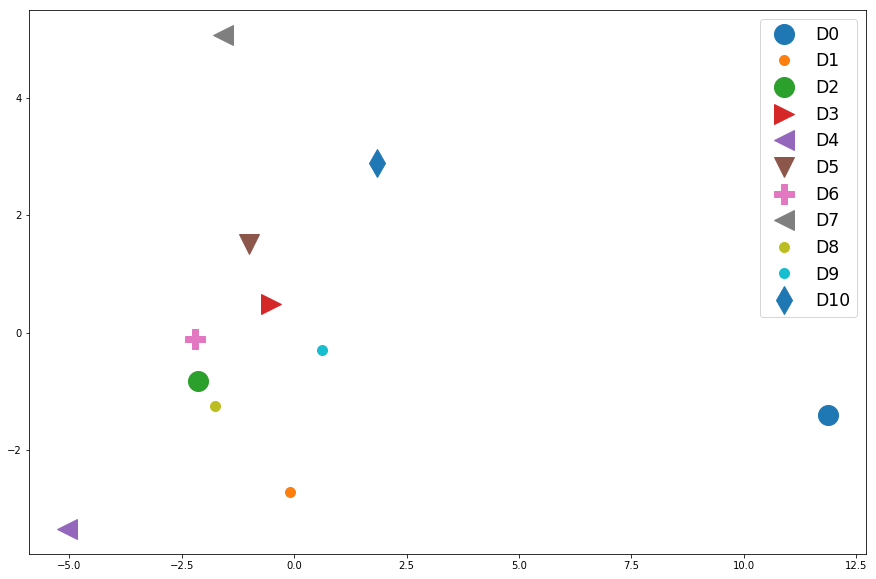
\includegraphics[scale=0.34]{doc2vec.png}
\caption{Documents listed in Section \ref{sec:publications} described by word embeddings and projected in a two-dimensional space by PCA. }
\label{fig:doc2vec}
\end{figure}


The second approach does not consider the order of the words to be relevant, but their frequency. It assumes words with similar meanings will occur in similar documents, and avoids considering the same terms or the same word sequences to relate documents. Topic models \citep{Deerwester1990} are the main methods that are based on this approach. \textbf{Probabilistic Topic Models (PTM)} \citep{Hofmann2001,Blei2003} are statistical methods based on bag-of-words that analyze the words of the original texts to discover the themes that run through them, how those themes are connected to each other, or how they change over time. PTM do not require any prior annotations or labeling of the documents. The topics emerge, as hidden structures, from the analysis of the original texts. These structures are topic distributions, per-document topic distributions or per-document per-word topic assignments. In turn, a topic is a distribution over terms that is biased around those words associated to a single theme. To better understand what topic means in this context, table \ref{table:sample-topics} shows the topics that have emerged when creating a topic model with the collection of example publications. Each topic is described by its five most representative words, i.e., those words most present in the documents that mainly contain each topic.

\begin{table}[!htbp]
\centering%
\begin{tabularx}{\linewidth}{HHHHH}
\toprule
\heading{Topic 0} & \heading{Topic 1} & \heading{Topic 2} & \heading{Topic 3} & \heading{Topic 4} \\
\midrule
\midrule
topic (27) & drug (15) & term (21) & synset (9) & document (1)\\
\midrule
document (20) & disease (9) & collection (11) & topic (8) & topic (1) \\
\midrule
base (17) & old (6) & document (10)  & document (8) & term (1)\\
\midrule
distribution (8) & PLWH (5) & value (9) & lingual (7) & base (1) \\
\midrule
model (8) & medication (5) & saturation (9) & category (6) & collection (1)\\
\midrule
\bottomrule
\end{tabularx}
\caption{Probabilistic topics created from the collection of articles listed in Section \ref{sec:publications}. For each topic the five most representative words are shown together with their normalized relevance (0-1000).}
\label{table:sample-topics}
\end{table}


This interpretable hidden structure annotates each document in the collection and these annotations can be used to perform deeper analysis about relationships between documents. Topic-based representations bring a lot of potential when applied over different IR tasks, as evidenced by recent works in different domains such as scholarly  \citep{Gatti2015}, health \citep{Lu2016, TapiNzali2017}, legal \citep{ONeill2017, Greene2016}, news \citep{He2017} and social networks \citep{Cheng2014a}. Moreover, some hybrid proposals have been recently used to model topics from word embeddings\citep{Dieng2020TopicMI}. Following the previous example, Figure \ref{doctopics} shows the articles projected in a two-dimensional space from their probabilistic topic-based representations. Unlike the distribution shown in Figure \ref{fig:doc2vec}, several documents now appear at the same position (e.g. $D_2-D_9$ and $D_3-D_4-D_6-D_8$). Being such a small collection of documents, 11 items, there are topics that are strongly present in the documents to differentiate them from the others. Thus, \textit{topic 1} groups documents $D_2$ and $D_9$ since it is related to the health domain. The same happens with documents $D_3$, $D_4$, $D_6$ and $D_8$ clearly focused on the efficient clustering of documents by probabilistic topics. In this case, \textit{topic 0} brings these documents together. The rest of the papers have a more balanced distribution of topics, indicating that they are less specific in a given domain.

\begin{figure}[!htbp]
\centering
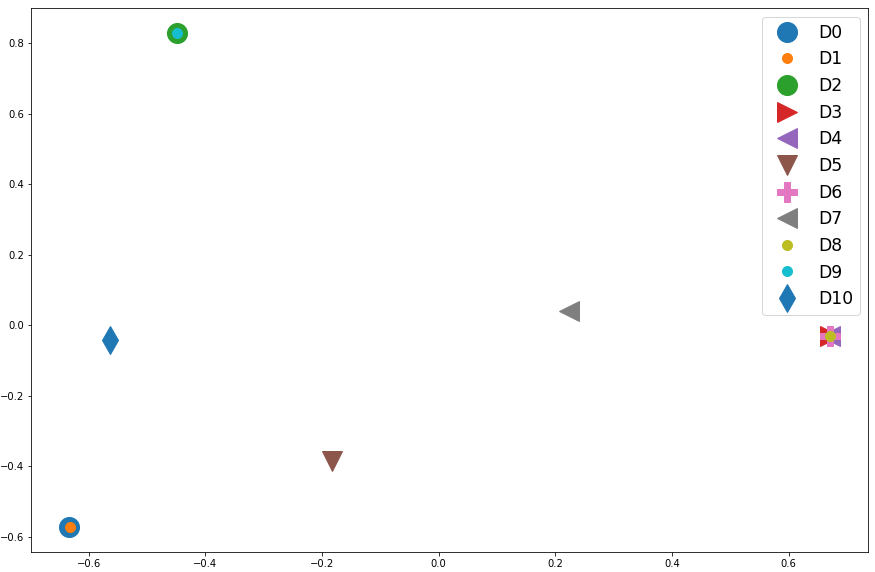
\includegraphics[scale=0.34]{doctopics.png}
\caption{Documents listed in Section \ref{sec:publications} described by probabilistic topics (Table \ref{table:sample-topics}) and projected in a two-dimensional space by PCA. }
\label{fig:doctopics}
\end{figure}

As just shown, the bag-of-words approach avoids the restriction of word sequences to relate documents. Documents that do not necessarily use the same words or in the same way can be strongly related if they mainly use the words that are more relevant for the same topic. The connection between documents is now the topic, not the word. Topic modeling provides an algorithmic solution to organize and annotate large collections of textual documents according to their topics. Our work is based on this approach since \textit{we are not only interested in representing words and documents, but we also seek structures that allows considering knowledge about the collection}.



\section{Techniques for Probabilistic Topic Models}\label{sec:techniques-prob-topics}

The simplest generative topic model proposed in the state of the art is \textit{Latent Dirichlet Allocation} (LDA) \citep{Blei2003}. Along with \textit{Latent Semantic Analysis} (LSA) \citep{Deerwester1990} and \textit{Probabilistic Latent Semantic Analysis} (pLSA) \citep{Hofmann2001} are part of the field known as topic modeling. They are well-known latent variable models for high dimensional data, such as the bag-of-words representation for textual data or any other count-based data representation. They try to capture the intuition that documents can exhibit multiple themes. Each document exhibits each topic in different proportion, and each word in each document is drawn from one of the topics, where the selected topic is chosen from the per-document distribution over topics. All the documents in a collection share the same set of topics, but each document exhibits these topics in a different proportion. Texts are described as a vector of counts with $W$ components, where $W$ is the number of words in the vocabulary. Each document in the corpus is modeled as a mixture over $K$ topics, and each topic $k$ is a distribution over the vocabulary of $W$ words. Formally, a topic is a multinomial distribution over words of a fixed vocabulary representing some concept. Depending on the function used to describe that distribution there are different algorithms to create topic models. LSA and pLSA propose a singular value decomposition. However, they have over-fitting issues. LDA was later proposed to overcome these issues. Influenced by the generative Bayesian framework it  suggests the use of a Dirichlet function as a continuous multivariate probability distribution parameterized by a vector of positive reals whose elements sum to 1.  It is continuous because the relative likelihood for a random variable to take on a given value is described by a probability density function, and is multivariate because it has a list of variables with unknown values. In fact, the Dirichlet distribution is the conjugate prior of the categorical distribution and multinomial distribution and allows LDA to infer topic distributions in texts that have not been used during training, unlike LSA and pLSA.

Topic models are not restrictive clustering models where each document is assigned to one cluster, but allow documents to exhibit multiple topics. The topics covered in a set of documents are discovered from the own corpus and feature vectors are topic distributions expressed as vector of probabilities.


\subsection{Document Similarity Calculation based on LDA}\label{sec:doc-sim-lda}

Since documents are described by topic distributions, the semantic similarity between two texts is based on the distance of their vector representations of the topics, which can be also seen as two probability mass functions. A commonly used metric is the \textit{Kullback-Liebler} (KL) divergence:

\begin{equation}
KL(P,Q) = \sum\limits_{i=1}^K p(x_{i}) \log \frac{p(x_{i})}{q(x_{i})}
\label{eq:kl}
\end{equation}
where  $K$ is the number of topics and $p,q$ are the topics distributions.

However, it presents two major problems: (1) when a topic distribution is zero, KL divergence is not defined and (2) it is not symmetric, which does not fit well with semantic similarity measures that are usually symmetric \citep{Rus2013}.

\textit{Jensen-Shannon} (JS) divergence \citep{Rao1982,Lin1991} solves these problems considering the average of the distributions as below \citep{Celikyilmaz2010}:

\begin{equation}
JS(P,Q) = \sum\limits_{i=1}^K p_{i}*\log \frac{2*p_{i}}{p_{i}+q_{i}}  +  \sum\limits_{i=1}^K q_{i}*\log \frac{2*q_{i}}{q_{i}+p_{i}}
\label{eq:jsdivergence}
\end{equation}


It can be transformed into a similarity measure as follows \citep{Dagan1998} :

\begin{equation}
sim_{JS}(D_i , D_j) = 10^{- JS(p,q)}
\label{eq:simjs}
\end{equation}
where  $D_i,D_j$ are the documents and $p,q$ the topic distributions of each of them.


\textit{Hellinger} (He) distance is also symmetric and is used along with JS divergence in various fields where a comparison between two probability distributions is required \citep{Blei2007a,Hall2008,Boyd-Graber2010}:

\begin{equation}
	He(P, Q) = \frac{1}{\sqrt{2}}\cdot\sqrt{\sum\limits_{i=1}^K (\sqrt{p_i} - \sqrt{q_i})^2)}
	\label{eq:hedistance}
\end{equation}

It can be transformed into a similarity measure by subtracting it from 1 \citep{Rus2013} such that a zero distance means max. similarity score and vice versa:

\begin{equation}
	sim_{He}(D_i, D_j) = 1 - He(p,q)
	\label{eq:simhe}
\end{equation}

However, all these metrics are not well-defined distance metrics, that is, they do not satisfy triangle inequality \citep{Charikar2002}. This inequality considers $d(x, z) <= d(x, y) + d(y, z)$ for a metric $d$ \citep{Griffiths2007} and places strong constraints on distance measures and on the locations of points in a space given a set of distances. As a metric axiom, the triangle inequality must be satisfied in order to take advantage of the inferences that can be deduced from it. Thus, if similarity is assumed to be a monotonically decreasing function of distance, this inequality avoids the calculation of all pairs of similarities by considering that if $x$ is similar to $y$ and $y$ is similar to $z$, then $x$ must be similar to $z$. 

\text{S2JSD} was introduced by \citep{Endres2003} to satisfy the triangle inequality. It is the square root of two times the $JS$ divergence:

%S2JSD formula
\begin{equation}
    S2JSD(P,Q) = \sqrt{2*JS(P,Q)}
\label{eq:s2jsd}
\end{equation}

\section{Research Areas}
\label{sec:research-topic}

This thesis aims to enable a semantic-aware exploration of the knowledge arising from large and multilingual document collections by exploiting the capabilities of topic models and their metric spaces. There are several research areas of ongoing related work. 

The first one is \textbf{topic creation and reuse}, key for understanding the steps needed to transform the unstructured data from a text into numerical values based on probabilistic topics. \textit{The way in which topic models are created and reused is crucial to addressing large-scale analysis}. 

The second area is \textbf{topic explainability}, which refers to the capacity of topics to capture and describe the content of a text. Topic explainability is important for \textit{making understandable the relationships that are derived from the inference of topic distributions}. 

The third area is \textbf{document similarity}, where the ability to measure the \textit{semantic difference between texts from the distance between their topic distributions is addressed}. 

Finally, the fourth area is \textbf{multilingual topics}, as we aim to explore collections of texts written in different languages through their topic-based relationships. A \textit{strategy to relate the topics of each language is tackled}. 

These four areas are closely related to each other. Having efficient thematic representations of texts, distance metrics based on shared themes, and mechanisms to abstract the particularities of a language to represent the themes, may help to organize large multilingual document collections.

Each area and its limitations are described below. A summary can be found in Table~\ref{table:limitations}.

\begin{table}[!htbp]
\centering%
\begin{tabularx}{\linewidth}{bbb}
\toprule
\heading{Area} & \heading{Scope}& \heading{Limitation} \\
\midrule
\midrule
topic creation & process texts and train topic models from large corpora & horizontal scalability (i.e. distributed computing) generally ignored in favor of vertical scalability (i.e. more computational power)  \\
\midrule
topic reuse & calculate topic distributions using existing topic models & no unified or standardized models for exchanging topic models \\
\midrule
topic explainability & describe and relate documents by topics & high dimensional models makes them difficult to interpret\\
\midrule
document similarity & compare topic distributions by measuring their distances & unaffordable complexity in huge collections  \\
\midrule
multilingual topics & topic distributions across languages & parallel or comparable training data required\\
\bottomrule
\end{tabularx}
\caption{Research areas and limitations.}
\label{table:limitations}
\end{table}



\subsection{Topic Creation and Reuse}
\label{sec:topic-reuse}

Textual content usually includes non-relevant information. Keeping only what can bring value for the involved agents (general consumers, experts, companies, investors...) becomes a challenge. A necessary first step before leveraging documents for knowledge-intensive tasks is to preprocess them following different techniques. Recent studies \citep{Westergaard2017} have shown that mining full-text articles gives consistently better results than only using sections or summaries. Given the size limitations and concise nature of summaries, they often omit descriptions or results that are considered to be less relevant but still are important for some IR tasks \citep{Divoli2012}.  Since this behavior is present in multiple domains, \textit{our interest is focused on processing full texts, not only summaries or parts of texts}, as we will show in the remainder of this thesis.

There is a broad set of algorithms able to analyze text for producing annotations at very different levels of granularity: from minimal units such as terms and entities, to descriptors at the level of the entire collection, such as summaries or topics. This includes methods and tools to perform Part-of-Speech (PoS) tagging, to recognize Named Entities (NER), or to create topic models following LDA or any other approach (e.g. LSA or pLSA). But their implementations have been designed to work in an isolated, non-collaborative way \citep{Manning2014TheToolkit, Agerri2014}. They have not paid special attention to facilitating their interoperability and they use closed data formats that increase the technological dependence and limits the reuse possibilities. For example, a topic model created by Mallet\footnote{\url{http://mallet.cs.umass.edu}} can only make inferences if it is used from Mallet itself or using its libraries, since \textbf{\textit{there is no unified or standardized format for distributing topic models}}. In that example, the fact that Mallet is implemented in Java prevents reusing their models from Python or any other programming language.

Some very recent approaches offer the creation and exploitation of topic models through an API based on libraries\footnote{\url{https://bab2min.github.io/tomotopy}} or web services\footnote{\url{https://github.com/D2KLab/ToModAPI}}\citep{Lisena:NLPOSS2020}. However they are focused on the operations that can be performed on the model rather than abstracting the topic model as a resource. Others provide local\footnote{\url{https://onnx.ai/}} or remote\footnote{\url{https://vespa.ai}} ecosystems to create and reuse learning models, but their data format is not open and cannot be (re)used out of the environment. To the best of our knowledge, the efforts made do not propose an unified model to exchange topic models, understood as an already accepted standards-based format. In this thesis we propose \textit{reusable topic models and a scalable framework to create and use them}.  
 

\subsection{Topic Explainability}
\label{sec:topic-explainability}

Even though the distance metrics mentioned in Section~\ref{sec:related-work} have been proposed and used in the SoA, making sense out of the similarity score based on compare topic distributions is not easy. As shown in figures \ref{fig:topic_distances} and \ref{fig:topic_distances2}, given a set of pairs of documents, their similarity scores vary according to the number of topics. So the distances between the same pairs fluctuate from being more to less distant when changing the number of topics, and are hence difficult to use to relate documents semantically. Understanding which of those distances is better for representing the underlying collection is a challenge.


\begin{figure}[]
\begin{subfigure}[b]{1.0\linewidth}
\centering
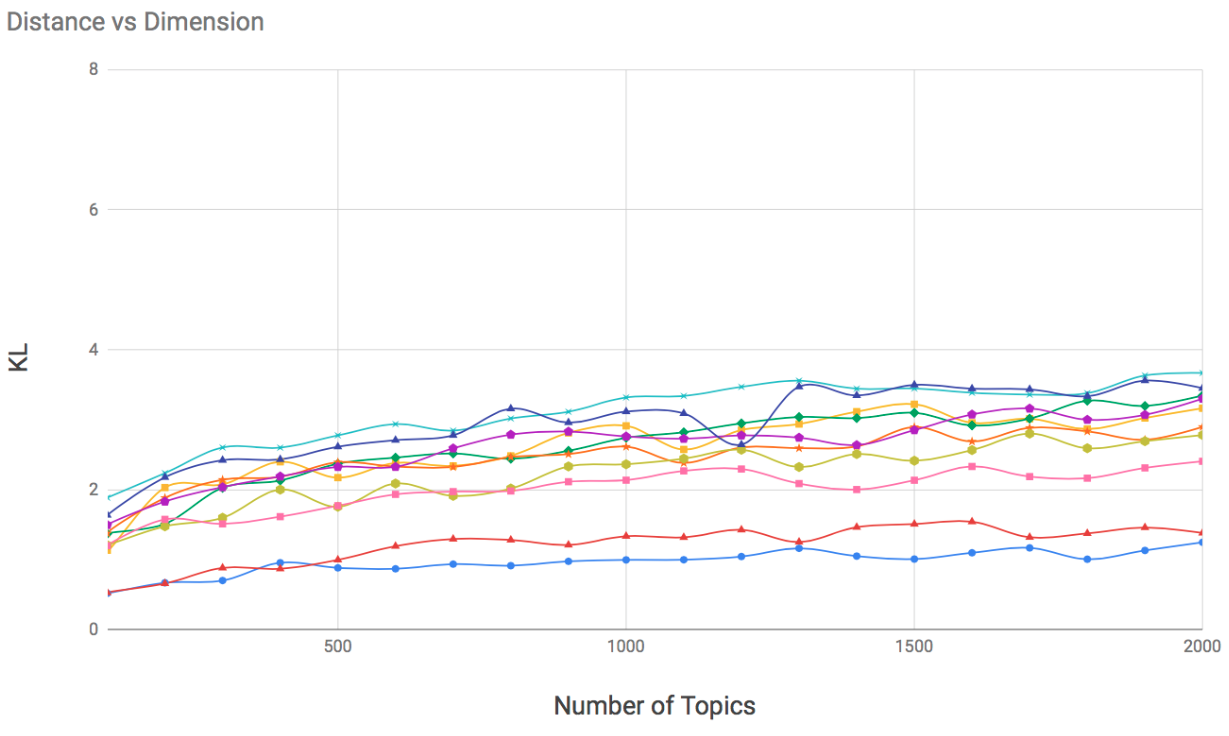
\includegraphics[width=\linewidth]{KL_100_2k.png}
\caption{Kullback-Liebler divergence}
\vspace{4ex}
\end{subfigure}
\begin{subfigure}[b]{1.0\linewidth}
\centering
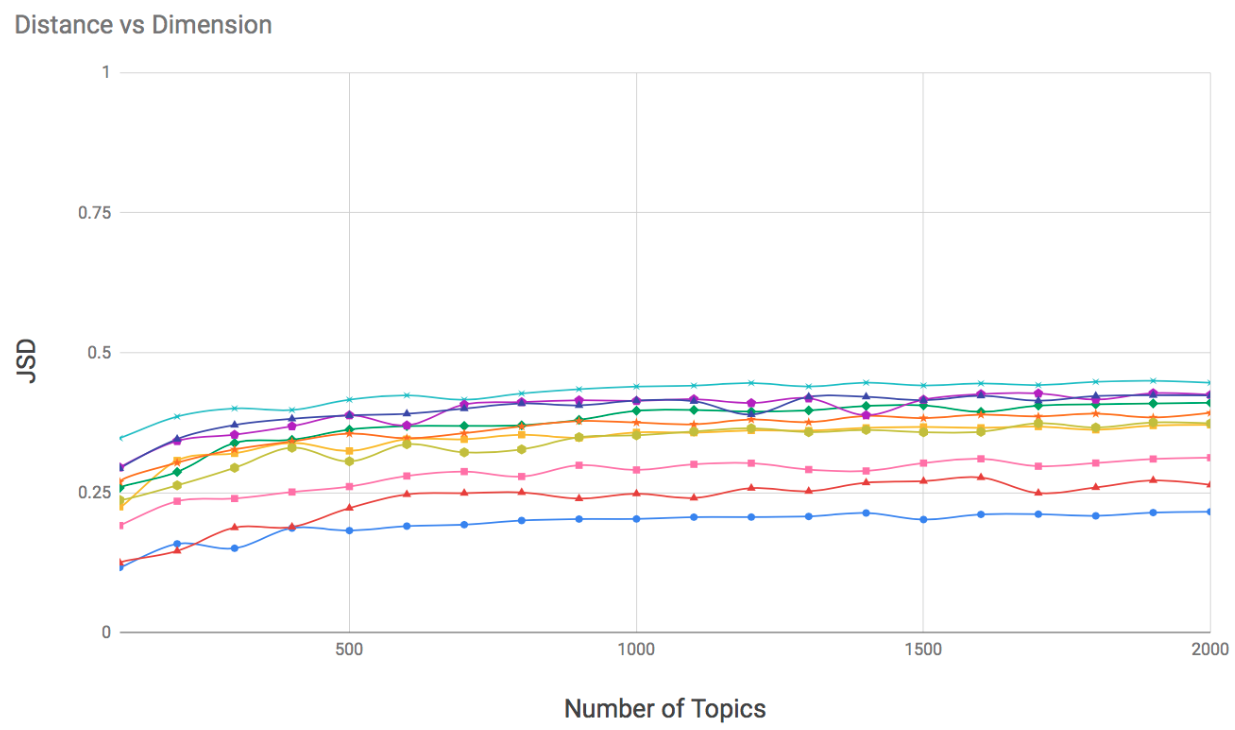
\includegraphics[width=\linewidth]{JSD_100_2k.png}
\caption{Jensen-Shannon divergence}
\vspace{4ex}
\end{subfigure}
\caption{Evolution of the distances based on KL (a) and JS (b) metrics between a set of document pairs when increasing the number of topics in the models  \citep{Badenes-Olmedo2020}.}
\label{fig:topic_distances}
\end{figure}

\begin{figure}[]
\begin{subfigure}[b]{1.0\linewidth}
\centering
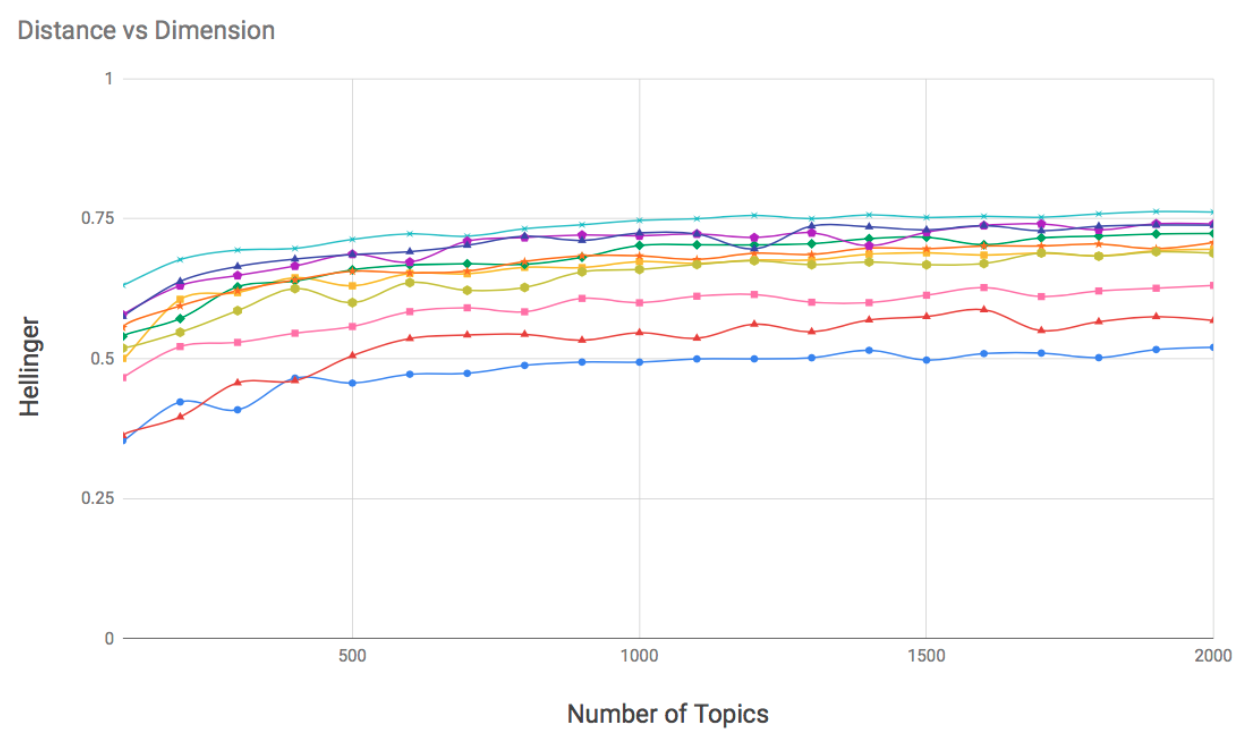
\includegraphics[width=\linewidth]{He_100_2k.png}
\caption{Hellinger distance}
\vspace{4ex}
\end{subfigure}
\begin{subfigure}[b]{1.0\linewidth}
\centering
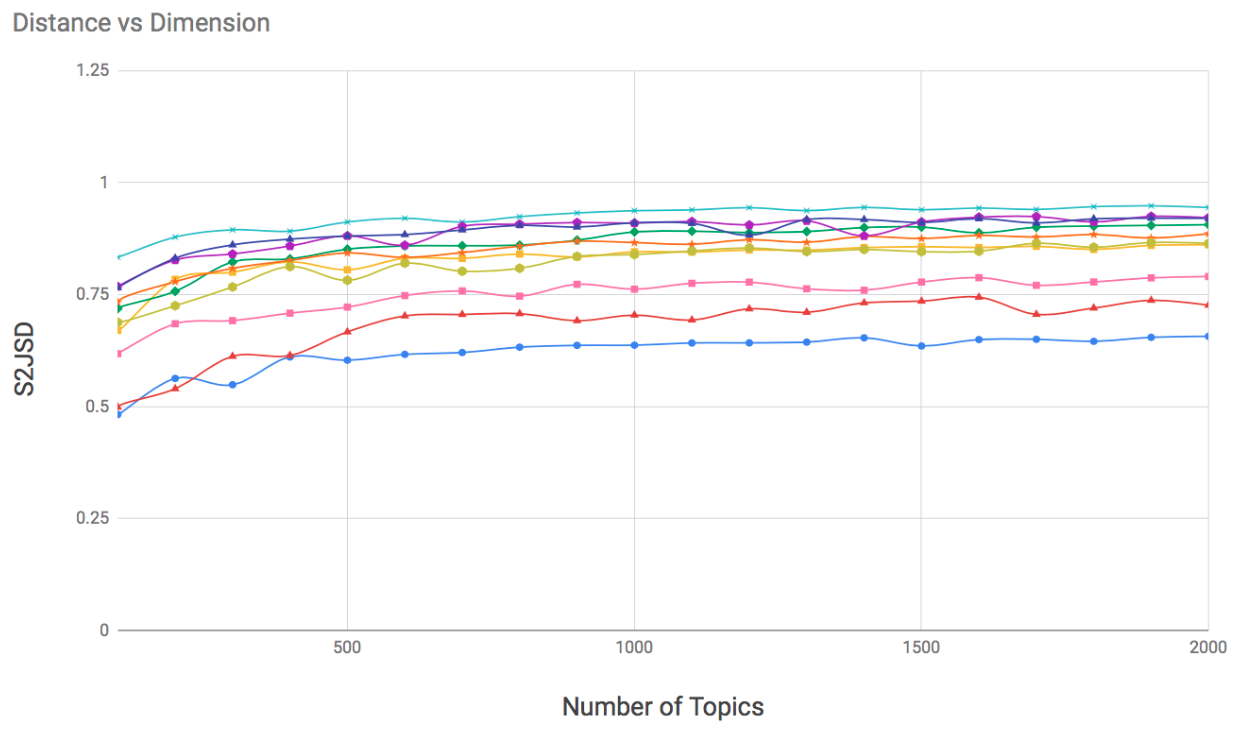
\includegraphics[width=\linewidth]{S2JSD_100_2k.png}
\caption{S2JSD distance}
\vspace{4ex}
\end{subfigure}
\caption{Evolution of the distances based on He (a) and S2JSD (b) metrics between a set of document pairs when increasing the number of topics in the models  \citep{Badenes-Olmedo2020}.}
\label{fig:topic_distances2}
\end{figure}


Distances between documents based on topic distributions generally increase as the number of dimensions of the space increases because it is a vector space. This is due to the fact that as the number of topics describing the model increases, the more specific the topics will be. Topics shared by a pair of documents can be broken down into more specific topics that are not shared by those documents. \textit{Document similarity is then dependent on the model used to represent documents when considering this type of metrics}. 

Each topic is drawn from a Dirichlet distribution with parameter $\beta$, while each document's mixture is sampled from a Dirichlet distribution with parameter $\alpha$. These two priors, $\alpha$ and $\beta$, are also known as hyper-parameters of a topic model and they set the probability that a document or a word, respectively, contains more than one topic. We know that absolute distances between documents vary when we tune those hyper-parameters differently, but we also see that ``relative distances" also change. Imagine that we have three documents, A, B and C, described by a topic model, M1. The distance from the topic distribution of A to B is less than from A to C. However, in a second topic model, M2, trained with the same documents than M1 but with different hyper-parameters, the distance from the topic distribution of A to C is less than to B (cross-lines in figures \ref{fig:topic_distances} and \ref{fig:topic_distances2}). This behaviour highlights the \textbf{\textit{difficulty of establishing absolute similarity thresholds and the complexity to measure distances taking into account all dimensions of a topic model}}. If we consider that documents are similar when their distance is lower than 0.2,for example, a pair of documents may be similar when they are represented in low-dimensional topic models, and not similar when high-dimensional models are used to represent them. Distance thresholds should be model-dependent rather than general, and metrics flexible enough to handle dimensional changes. In this thesis we go beyond the thematic and low-dimensional feature space created by topic models and propose a \textit{hierarchical feature space suitable for big real-world data sets, where documents are only described by their most relevant topics}.


\subsection{Document Similarity}
\label{sec:document-similarity}

In addition, document similarity comparisons are too costly to be performed in huge collections of data and require more efficient approaches than having to calculate all pairwise similarities. Using a naive approach creating a similarity matrix with all document comparisons takes $O(n^2)$ time (where $n$ is the number of documents), so obtaining all possible pairs of similarities in a large collection of documents (e.g. a corpus of 32 million patents) can be unfeasible because of the quadratic cost of comparing every pair of elements. Many different approaches have been proposed to reduce this complexity. For instance, computation can be approximated by a nearest neighbors (ANN) search problem \citep{Indyk1998}. ANN search is an optimization problem that finds nearest neighbors of a given query in a metric space of $n$ points. 

Due to the low storage cost and fast retrieval speed, hashing is one of the most popular solutions for ANN search \citep{Zhen2016}. This technique transforms data points from the original feature space into a binary-code space, so that similar data points have larger probability of collision (i.e. having the same hash code). This type of formulation for the document similarity comparison problem has proven to yield good results in the metric space \citep{Krstovski2011} due to the fact that ANN search has been designed to handle distance metrics (e.g. cosine, Euclidean, Manhattan). But distance metrics between topic distributions should be information-theoretically motivated metrics (e.g. Hellinger, Kullback-Leibler divergence, Jensen-Shannon divergence) since they compare density functions. 

These challenges can be tackled by hashing methods based on clusters of topics to measure similarity, instead of directly using their weights. Hashing methods transform the data points from the original feature space into a binary-code Hamming space, where the similarities in the original space are preserved. They can learn hash functions (data-dependent) or use projections (data-independent) from the training data \citep{Wang2016}. Data-independent methods, unlike data-dependent ones do not need to be re-calculated when data changes, i.e. adding or removing documents to the collection. Taking large-scale scenarios into account (e.g. Document clustering, Content-based Recommendation, Duplicate Detection), data independency is a key feature along with the ability to infer hash codes individually (for each document) rather than on a set of documents. Data-independent hashing methods depend on two key elements: (1) data type and (2) distance metric. For vector-type data, as introduced in section \ref{sec:related-work}, based on $l_p$ distance with $p \epsilon [0,2)$ lots of hashing methods have been proposed, such as p-stable Locality-Sensitive Hashing (LSH) \citep{Datar2004}, Leech lattice LSH \citep{Andoni2006}, Spherical LSH \citep{Terasawa2007}, and Beyond LSH \citep{Andoni2014}. Based on the $\theta$ distance many methods have been developed such as Kernel LSH \citep{Kulis2012} and Hyperplane hashing \citep{Vijayanarasimhan2014}. But only few methods handle density metrics in a simplex space, where topic distributions are projected. A first approach transformed the $He$ divergence into an Euclidean distance so that existing ANN techniques, such as LSH and k-d tree, could be applied \citep{Krstovski2013a}. But this solution does not consider the special attributions of probability distributions, such as Non-negative and Sum-equal-one. Recently, a hashing schema \citep{Mao2017} has been proposed taking into account the symmetry, non-negativity and triangle inequality features of the S2JSD metric for probability distributions. For set-type data, Jaccard Coefficient is the main metric used. Some examples are K-min Sketch \citep{Li2012}, Min-max hash \citep{Ji2013}, B-bit minwise hashing \citep{Li2010b} and Sim-min-hash \citep{Zhao2013}.

All of them have demonstrated efficiency in the search for similar documents, but none of them considers the search for documents (1) by thematic areas or (2) by similarity levels, nor they offer (3) an \textbf{\textit{explanation about the similarity obtained beyond the vectors used to calculate it}}. In addition, binary-hash codes drop a very precious information: the topic relevance. This thesis proposes a \textit{hash function-based approach that allows efficiently searching for related documents while maintaining topic-based annotation, preserving the notion of why two documents are related}.


\subsection{Multilingual Topic Alignment}
\label{sec:multi-topic-alignment}

When the IR task is also cross-language, document retrieval must be independent of the language of the user's query. At execution time, the query in the source language is typically translated into a target language with the help of a dictionary or a machine-translation system. But for many languages we may not have access to translation dictionaries or a full translation system, or they can be expensive to execute, or expensive to train (lot of data required) in an online search system. In such situations it is useful to rely on smaller annotation units derived from the text so the full content does not need to be translated, for instance by finding correspondences with regard to the topics that are present in both the query and the documents being searched.

Some methods use document-aligned corpora, where documents are grouped and constrained to the same topic distribution during training to align the different languages \citep{mimno-etal-2009-polylingual, Ni2009, Fukumasu2012, Zhang2013}, or theme-aligned corpora, where similar themes and ideas appear in all languages \citep{Graber2009}. Multilingual Probabilistic Topic Models (MuPTM) \citep{Vulic2015} emerged in this area as a group of language-independent generative machine learning models that can be used on theme-aligned multilingual texts. They are based on LDA, adding supervised associations between languages by using \textit{parallel} corpora, with sentence-aligned documents (e.g. Europarl\footnote{https://ec.europa.eu/jrc/en/language-technologies/dcep} corpus), or \textit{comparable} corpora, with theme-aligned documents (e.g. Wikipedia\footnote{https://www.wikipedia.org/} articles), in multiple languages. Once a MuPTM has been generated, documents can be represented by data points in a single feature space based on topics to detect similarities among them exploiting inference results and using distance metrics. Due to its generic language-independent nature and the power of inference on unseen documents, MuPTM's have found many interesting applications in many different cross-lingual tasks. They have been used on cross-lingual event clustering \citep{Smet2009}, document classification \citep{10.1007/978-3-642-20841-6_45, Ni:2011:CLT:1935826.1935887},  semantic similarity of words \citep{mimno-etal-2009-polylingual, Vulic:2012:DHC:2380816.2380872}, information retrieval \citep{10.1007/978-3-642-36973-5_9, ganguly-etal-2012-cross}, document matching \citep{Platt:2010:TDR:1870658.1870683, zhu-etal-2013-building}, and others. 

There are also methods based on word alignments from bilingual dictionaries instead of aligned corpora. Topic models emerge as distributions over crosslingual equivalence classes of words \citep{Jagarlamudi2010, zhang-etal-2010-cross, shi-etal-2016-detecting, hao-paul-2018-learning}. Others propose to translate only the words used to characterize the topics across the languages, such as anchor words \citep{NEURIPS2018_28b9f8aa} or top words \citep{yang2019multilingual}. A recent approach is placed between word and document alignments since it proposes crosslingual topic models using the language-independent categories assigned to each Wikipedia article \citep{2020arXiv200911207P}. Instead of using bags-of-words to represent texts, which would be language dependent, it explores the references of each article and represents them through bags-of-links, using the categories of each reference to represent the texts.

However, \textbf{\textit{the requirement of parallel/comparable corpora or dictionaries limits the usage of these models in many cross-lingual situations}}. There are not many document collections that can be used for training since large parallel corpora are rare in most of the use cases, especially for languages with fewer resources. Moreover, in order to incorporate new languages or update the existing associations, these models must be (re)trained with documents from all languages at the same time, making it difficult to scale to large corpora \citep{Hao2018, Moritz2017}. Inspired by the work of \citep{Boyd-Graber2010}, where the use of concepts to align topics from different languages is proposed, we take MuPTM a step further by making it cross-lingual through representations based on topic hierarchies. We do not only use conceptual representations of the top words in a topic, but we group the words hierarchically by relevance and compare their conceptual representations at those levels. Documents are represented by topics described with language independent concepts and multilingual corpora can efficiently be browsed without the need for translation. In this thesis we propose to \textit{automatically infer cross-lingual topics to browse multi-lingual document collections without the need for parallel or comparable corpora}.

A summary with the proposals of this thesis to overcome the limitations of each research area (described in table \ref{table:limitations}) can be found in table \ref{table:proposals}. 

\begin{table}[!htbp]
\centering%
\begin{tabularx}{\linewidth}{bb}
\toprule
\heading{Area} & \heading{Proposal} \\
\midrule
\midrule
topic creation and reuse & distributed framework to create and  (re)use topic models\\
\midrule
topic explainability & hierarchical feature space suitable for big real-world data sets, where documents are only described by their most relevant topics\\
\midrule
document similarity & hash function-based algorithm that allows  searching for related documents efficiently while maintaining topic-based annotation, preserving the notion of why two documents are related  \\
\midrule
multilingual topics & cross-lingual topics based on hierarchical representations of concepts to browse multi-lingual document collections without the need for parallel or comparable corpora\\
\bottomrule
\end{tabularx}
\caption{Research areas and proposals.}
\label{table:proposals}
\end{table}	

% this file is called up by thesis.tex
% content in this file will be fed into the main document

%: ----------------------- introduction file header -----------------------
\chapter{Research Objectives}\label{ch:hypothesis}

\graphicspath{{hypothesis/figures/}}

% -------------------------------------------------------------
% -- Research Objectives 
% -------------------------------------------------------------

The work presented in this thesis aims to facilitate the exploration of huge collections of multilingual documents through thematic associations inferred from their content. Each of the challenges arising from this objective defines a working dimension and guides the research carried out in this thesis.

% Hacer referencia a secciones de los capitulos 1 y 2 cuando estén terminados
The first dimension focuses on \textbf{scalability}, in order to create the text processing flows that are required to create or apply learning models. The workload required to process a corpus varies according to the number of documents, the length of texts and the kind of knowledge (annotations) that need to be inferred from the text. If the design of the workflow is scalable, there is no need to modify the processing logic when working with larger collections of documents, since adding a reasonable amount of computational resources is enough to perform it. These resources can be machines (i.e horizontal scaling) or processing units (e.g CPU, RAM) in an existing machine (i.e vertical scaling). 

The second dimension covers the \textbf{representativeness} of the text annotations when projected into spaces where they are manipulated. The idea behind these spaces is to represent documents as points (or vectors in a vector space) that are close together when the texts are semantically similar, and far apart when they are semantically distant. The ability of these spaces to create meaningful representations is also studied in this work.

In the third dimension, data structures that efficiently \textbf{sort} texts from their representations based on probabilistic topics are studied. Divisions of space into semantically-related regions are convenient to allow browsing large document collections. The \textit{representativeness} covered in the previous dimension enables the interpretation of the relations and regions obtained.

And finally, the fourth dimension handles the \textbf{multilingualism} of collections that contain documents in several languages. On a multilingual space, documents are described and related across languages.

This chapter introduces our main hypothesis (section \ref{sec:research-hypothesis}), and the associated research challenges (section \ref{sec:research-challenges}), and presents the research methodology (section \ref{sec:research-methodology}).

\section{Research Hypotheses}\label{sec:research-hypothesis}

We define our main hypothesis as follows:

\textbf{Hypothesis 1} \textit{Large multilingual document collections can be automatically analyzed to discover appropriate thematic relations that facilitate a semantically-enabled text browsing}.

Our hypothesis can be divided into four different sub-parts, which are related to the aforementioned scalability, representativeness, sorting, and multilinguality dimensions respectively. First, by \textit{distributing both natural language processing tasks and representational models we can efficiently process huge collections of documents (\textbf{H1.1})}.

% topics no se ha utilizado hasta ahora?
Second, we can \textit{semantically relate documents by comparing their most relevant topics (\textbf{H1.2})}. Furthermore, for this purpose we hypothesize that the use of \textit{topic hierarchies (\textbf{H1.2.1}) and similarity metrics based on relevance levels (\textbf{H1.2.2}) can help quantifying the semantic distance between texts}. Third, by \textit{dividing the representational space into regions based on topics and relevance levels we can search for related documents without having to calculate all pairwise comparisons and without losing the ability to rely on topics for further processing (\textbf{H1.3})}.

And finally, \textit{by abstracting the topic representations into concept-based descriptions across languages we can relate documents in various languages without having to translate them (\textbf{H1.5})}.

A summary of the hypotheses and how they tackle our research dimensions can be found in Table~\ref{table:hypotheses}.

\begin{table}[!htbp]
\centering%
\begin{tabularx}{\linewidth}{bs}
\toprule
\heading{Hypothesis} & \heading{Research Dimension } \\
\midrule
\midrule
H1: Large multilingual document collections can be automatically analyzed to be semantically-browsed through thematic relations & D1: Scalability, D2: Representativeness, D3: Sorting, D4: Multilingualism \\
\midrule
H1.1: it is possible to efficiently annotate documents on a large scale by distributing natural language processing tasks and representation models & D1: Scalability\\
\midrule
H1.2: it is possible to semantically relate texts from their most relevant topics & D2: Representativeness\\
\midrule
H1.3: it is possible to find documents with similar topic distributions without calculating all pairwise comparisons and without losing the ability to explore them through their topics & D3: Sorting\\
\midrule
H1.4: it is possible to relate documents in different languages without having to translate them using language agnostic concepts from their main topics & D4: Multilingualism\\
\bottomrule
\end{tabularx}
\caption{Hypotheses and research dimensions.}
\label{table:hypotheses}
\end{table}


\section{Research Challenges}\label{sec:research-challenges}

Several research challenges emerge from these hypotheses. First, in order to facilitate reusing existing topic models by processing systems with different architectures and technological stacks, we need to define \textit{topic-model programming interfaces}. Second, in order to describe and thematically relate documents, we must address how to produce \textit{explainable topic-based associations}. Third, by working with huge collections of documents described by topics, we need to handle \textit{large-scale comparisons of topic distributions}. Finally, in order to explore multilingual document collections from shared topic-based representational spaces, we have to provide \textit{automatic cross-lingual topic alignment}. Each of these research challenges are described below and covered throughout this thesis.

\subsection{Topic-model Programming Interface}

Although some initiatives to standardize the format of machine-learning models and to provide tools that facilitate their transformation among the most widespread proprietary formats already exist in the literature, there are still some software restrictions that can limit their reuse. These models may hold certain software dependencies that e.g. force using a specific version of a programming language (python2 vs python3\footnote{\url{https://www.python.org}}) or an operating system (e.g., linux kernel vs on-cloud environments\footnote{\url{https://vespa.ai}}) to load them or to launch the service that deploys them (e.g., ONNX\footnote{\url{https://onnx.ai}}). This limits their ability to be reused in domains that are not familiar with these technological stacks. \textit{Integrating pre-trained topic models into general-purpose systems is not easy \textbf{(RCInterface1)}}.


Topic models, as many other machine learning models, may be distributed in a proprietary or standard format with software dependencies or by directly providing the data. However, \textit{there is no standard way to specify the topics and the operations that can be performed on them \textbf{(RCInterface2)}}. Sometimes topics are described by the top ten or five most relevant words, and occasionally these word lists are not accompanied by weights, making a density-based analysis impossible. These differences in presenting the models can sometimes limit their reusability if they cannot infer new topic distributions even when the learning algorithm allows for it.


\subsection{Explainable Topic-based Associations}

In order to facilitate the exploration of document collections, vector space models are often used to semantically relate texts based on their word distributions. These models first create a dictionary with the words used in the collection, and then represent  documents by vectors whose dimensions correspond to each word in the dictionary. In large collections, these models need to be adapted to make operations on vectors more manageable. As a result, a new abstraction method based on topics emerged that reduces the dimensions of vectors. Topics are described by word distributions over the entire vocabulary and documents by vectors containing topic distributions. Despite the extensive use of these representation models, \textit{there is no common criteria for identifying the most representative topics in a document \textbf{(RCExplainable1)}}. 

In addition, since similarity metrics over this representation space are based on accumulating the difference in topic densities, \textit{it is difficult to explain the distance between topic distributions \textbf{(RCExplainable2)}}. And, unless a minimum distance threshold is defined or a n-top topics agreed, \textit{there is no common criterion for determining whether two documents are related \textbf{(RCExplainable3)}}.  


\subsection{Large-scale Comparisons of Topic Distributions}

There are many scenarios where finding related documents in a huge corpus is desirable (e.g. a researcher doing literature review, or an R\&D  manager analyzing project proposals). Experts can benefit from discovering those connections to achieve these goals, but brute-force pairwise comparisons are not computationally adequate when the size of the corpus is too large. Some algorithms in the literature divide the search space into regions containing potentially similar documents, which are later processed separately from the rest in order to reduce the number of pairs compared. However, \textit{there are no mechanisms that efficiently partition the topic-based search space without compromising the ability for thematic exploration \textbf{(RCComparison1)}}.

In addition, documents from the same region should be compared and \textit{there are no similarity metrics that compare partial distributions of topics \textbf{(RCComparison2)}}.


\subsection{Automatic Cross-lingual Topic Alignment}

% actualizar referencias a secciones del sota
With the ongoing growth in the number of texts in different languages, we need annotation methods that enable browsing multi-lingual corpora. As discussed in section \ref{ch:soa}, multilingual probabilistic topic models have recently emerged as a group of semi-supervised machine learning models that can be used to perform thematic explorations on collections of texts in multiple languages. However, \textit{there are no approaches that abstract the representation of probabilistic topics in language-independent spaces without translating texts or aligning documents \textbf{(RCCrossLingual1)}}. Existing approaches require parallel or comparable training data to create a language-independent space. 

A summary of the challenges covered in this work and how they map to the hypotheses is presented in table  \ref{table:challenges}.

\begin{table}[!htbp]
\small
\centering%
\begin{tabularx}{\linewidth}{bb}
\toprule
\heading{Research Challenge} & \heading{Hypotheses} \\
\midrule
\midrule
RCInterface1: integrating pre-trained topic models into general-purpose systems is not easy & H1.1: documents can be efficiently annotated on a large scale by distributing natural language processing tasks and representation models\\
\midrule
RCInterface2: there is no standard presentation of topics that facilitates their reuse & H1.1: documents can be efficiently annotated on a large scale by distributing natural language processing tasks and representation models\\
\midrule
RCExplainable1: there is no common criteria for identifying the most representative topics in a document & H1.2: texts can be semantically related from their most relevant topics, H1.3: documents with similar topic distributions can be found without calculate all pairwise comparisons and without losing the ability to explore them through their topics \\
\midrule
RCExplainable2: it is difficult to understand the distance between topic distributions & H1.2: texts can be semantically related from their most relevant topics\\
\midrule
RCExplainable3: there is no common criterion for determining whether documents are related & H1.2: texts can be semantically related from their most relevant topics\\
\midrule
RCComparison1: there are no mechanisms that efficiently partition the topic-based search space without compromising the ability for thematic exploration & H1.3: documents with similar topic distributions can be found without calculate all pairwise comparisons\\
\midrule
RCComparison2: there are no similarity metrics that compare partial distributions of topics & H1.3: documents with similar topic distributions can be found without calculate all pairwise comparisons\\
\midrule
RCCrossLingual1: there are no approaches to abstract probabilistic topics in language-independent spaces without translating texts or aligning documents  & H1.4: documents in different languages can be related without having to translate them using language agnostic concepts from their main topics\\
\bottomrule
\end{tabularx}
\caption{Open Research Challenges and Hypotheses.}
\label{table:challenges}
\end{table}

\section{Research Methodology}\label{sec:research-methodology}

The research presented in this thesis is based on four dimensions or research areas as discussed in section \ref{sec:research-challenges}. Each one is motivated by different research problems that we need to solve in order to achieve our ultimate goal of making it easier to explore large multilingual document collections through their topics. Once a dimension is tackled, the next one is considered, and so on. This iterative and incremental methodology allows  refining the research results by evaluating them with more experiments and addressing increasingly complex research problems.

Figure \ref{fig:dimensions} shows the dimensions on which the research of this thesis has been built. The top of the pyramid is only reached once the lower dimensions are dealt with successfully. They are presented as a chain of four steps. The first step describes the motivation to perform a given task coming from real-world problems that we had to deal with, and is represented by a brown arrow. In the context of this task, the research problem arises and is framed by a pink arrow. For each of them a solution is proposed and evaluated according to a specific criterion. The proposed solution is represented by a green arrow and the evaluation with a blue arrow. Once a proposal has been validated, the next dimension of the pyramid is achievable and all the previous research problems are added to the new research problem as conditions to be taken into account.

Technical objectives (i.e., develop a new resource) or research objectives (i.e., discover the solution to a problem) guide the solution proposal before moving on to the next dimension. They are presented below, organized by the research problem associated with each dimension.


\subsection{Scalable Creation and Inference of Topics}

This first dimension arose when we had to analyze a huge collection of documents describing research and innovation projects to discover which research areas are being addressed, measure their presence in the collection, and characterize them so their presence can be inferred in unseen documents. Such a high volume of data made difficult to process it manually, so we needed to automate the required processing to draw insights from it. Probabilistic topics allow describing research areas, so we defined a \textit{distributed text-processing model for creating large probabilistic topic models (\textbf{RO1})} and a \textit{web service template to distribute them (\textbf{RO2})}. In this way, the models themselves could be easily integrated into scalable text processing pipelines. As a result, we created a \textit{platform for large-scale text analysis (\textbf{TO1})}, and produced a \textit{model-as-a-service repository with pre-trained topic models (\textbf{T02})}. The efficiency of this solution was validated by processing a corpus of 100,000 documents collected from the CORDIS dataset\footnote{\url{https://data.europa.eu/euodp/es/data/dataset/cordisH2020projects}}, which contains descriptions of projects funded by the European Union under a framework programme since 1990 \citep{Badenes-Olmedo2017}. 

The main contributions under this dimension are described in Chapter \ref{ch:scalability} as follows:
\begin{itemize}
\item a software architecture to process big volumes of textual documents in a distributed and decoupled manner;
\item the definition of a model-as-a-service template for probabilistic topic models;
\item an implementation of the architecture, librAIry, following those design principles.
\end{itemize} 


\subsection{Explainable Topic-based Associations}

In the second dimension we needed to browse scientific papers through their content-based relations. The problem of massively annotating documents with topic distributions came up. We had to \textit{create annotations based on topic models in a way that was computationally affordable and enabled a semantic-aware exploration of the knowledge inside them (\textbf{RO3})}. Once documents were annotated, a \textit{metric that compares documents and facilitates their interpretation from topic annotations (\textbf{RO4})} was required. As a result, we integrated \textit{the annotation method into the topic model service (\textbf{TO3})} and implemented a text comparison metric based on partial representations of topics. These proposals were validated by classifying 500,000 scientific articles from the Open Research Corpus\footnote{\url{https://allenai.org/data/open-research-corpus}} in domains such as Computer Science, Neuroscience and Biomedicine \citep{Badenes-Olmedo2017b, Badenes-Olmedo2017c, Badenes-Olmedo2019b}. 

The main contributions under this dimension are described in Chapter \ref{ch:explainability} as follows:
\begin{itemize}
\item a clustering algorithm based on probabilistic topic distributions;
\item a hash function to transform topic distributions into topic hierarchies;
\item a similarity metric based on topic sets.
\end{itemize} 

\begin{figure}[!htbp]
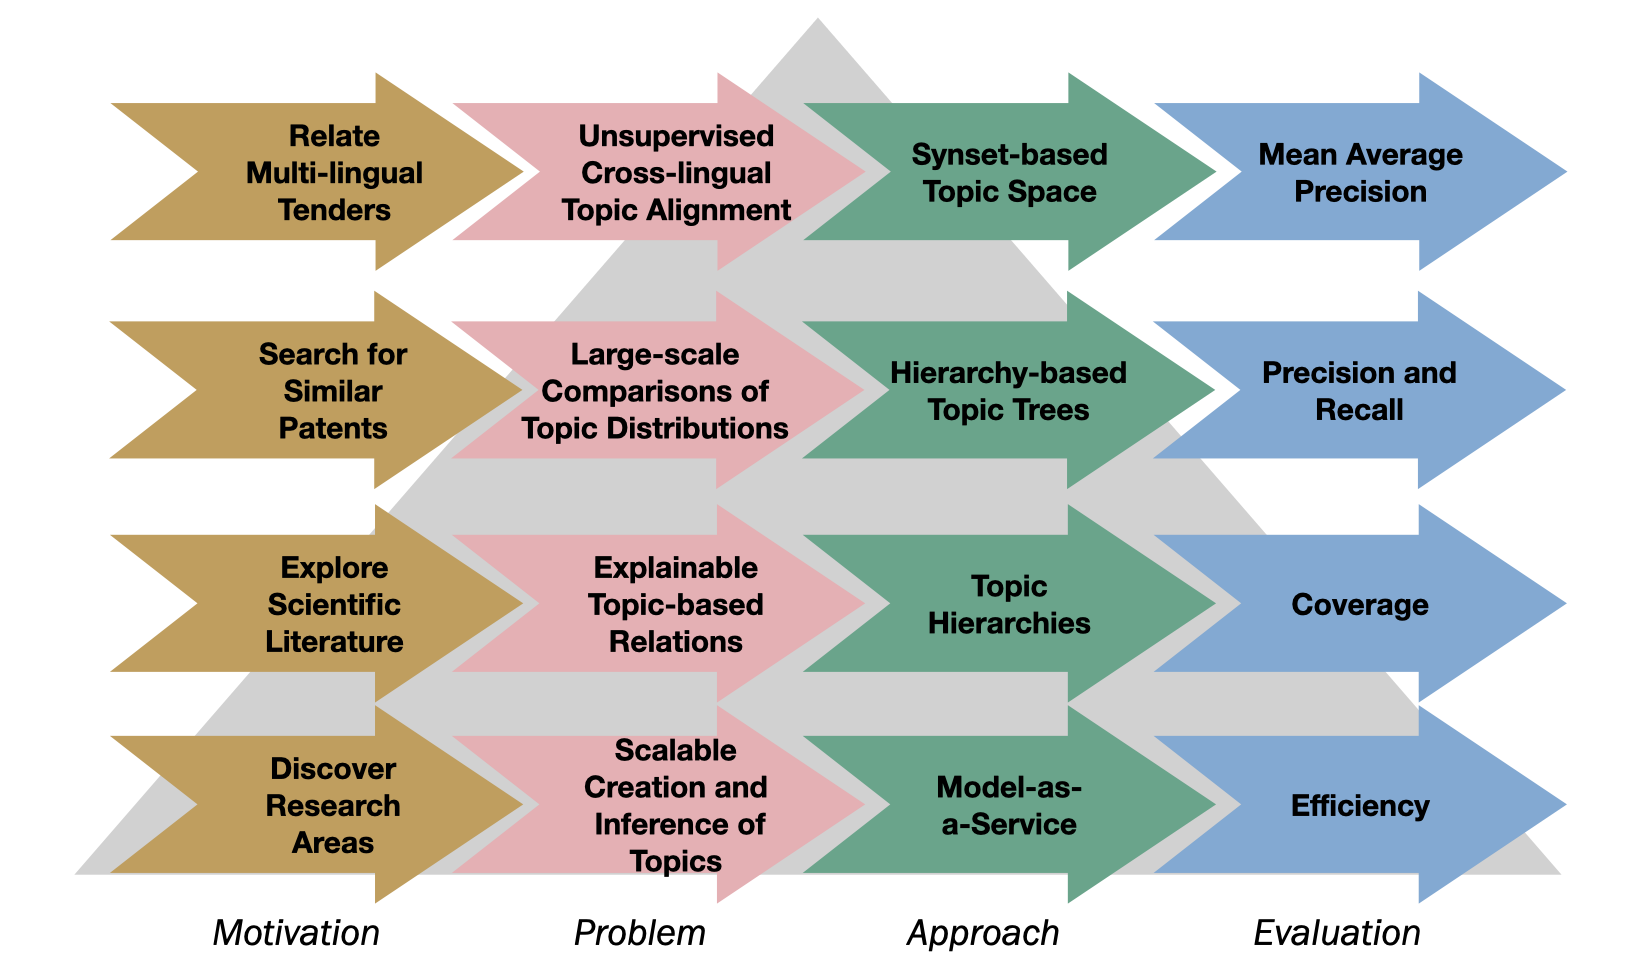
\includegraphics[scale=0.25]{dimensions.png}
\centering
\caption{Research dimensions of the thesis. The first ones must be overcome before reaching higher dimensions. }
\label{fig:dimensions}
\end{figure}

\subsection{Large-scale Comparisons of Topic Distributions}

This dimension covered the search for similar documents based on their most relevant topics. Thanks to having dealt with the above two dimensions, large collections of documents could be annotated with topic hierarchies and text distances could be measured from their annotations. Now, the aim was to find similar documents without losing the exploratory capacity offered by topics. Similarity comparisons were too costly to be performed in such huge collections of data and required more efficient approaches than having to calculate all pairwise similarities. We applied \textit{techniques based on approximate nearest-neighbors to organize documents in regions with similar topic hierarchies (\textbf{RO5})}. As a result, we developed \textit{a system to automatically find similar documents (\textbf{TO4})}. It was validated on a collection of one million texts retrieved from the United States patents corpus\footnote{\url{https://www.uspto.gov/ip-policy/economic-research/research-datasets}}. The relations between patents derived from their manual categorization were compared with those automatically obtained from their topic distributions \citep{Badenes-Olmedo2020, Badenes-Olmedo2019b}. 

The main contributions under this dimension are described in Chapter~\ref{ch:comparisons} as follows:
\begin{itemize}
\item a data structure to partition the search space and organize documents described by topic hierarchies;
\item a corpus browser that leverages these representations to automatically relate documents.
\end{itemize} 


\subsection{Automatic Cross-lingual Topic Alignment}

Finally, a new dimension on top of the previous ones emerged to relate texts coming from different languages. In particular, since document relations were based on their topics, this dimension was focused on aligning topics without supervision from models trained with texts in different languages. Since each language defined its own vocabulary, the topics were model-specific and could not be directly compared. We abstracted the \textit{topic representations to create a single space out of the particularities of the language (\textbf{RO6})}. This approach was validated on the English, Spanish, French, Italian and Portuguese editions of the JCR-Acquis\footnote{\url{https://ec.europa.eu/jrc/en/language-technologies/jrc-acquis}} corpora and revealed promising results on classifying and sorting documents by similar content across languages \citep{Badenes-Olmedo2019, Badenes-Olmedo2019b}. 

The main contributions under this dimension are described in Chapter~\ref{ch:multilinguality}, as follows: 
\begin{itemize}
\item an algorithm to represent probabilistic topics using concept sets;
\item a repository of aligned topic models from the English, Spanish, French, Italian and Portuguese editions of the JRC-Acquis corpus.
\end{itemize}

Table \ref{table:objectives} summarizes the research objectives (ROs), technical objectives (TOs) and connects them with the research challenges (RCs) from Table \ref{table:challenges}.


\begin{table}[!htbp]
\centering%
\small
\begin{tabularx}{\linewidth}{bs}
\toprule
\heading{Research Objective} & \heading{Research Challenge}\\
\midrule
\midrule
RO1: Define a distributed text-processing model for creating large probabilistic topic models  & RCInterface1 \\
\midrule
RO2: Define a template to package probabilistic topic models as web services & RCInterface2\\
\midrule
RO3: Define annotations based on topics that enable a semantic-aware exploration of the knowledge inside a corpus & RCExplainable1\\
\midrule
R04: Define a metric based on topic annotations that compares documents and facilitates their interpretation & RCExplainable2, RCExplainable3\\
\midrule
RO5: Define nearest-neighbor techniques to organize documents in regions with similar topic hierarchies & RCComparison1, RCComparison2\\
\midrule
R06: Define a transformation of the topic-based annotations to create a unique representational space out of the particularities from each language & RCCrossLingual1\\
\midrule
TO1: Create a platform for large scale text processing & RCInterface1, RCInterface2\\
\midrule
T02: Create a repository of Topic-based web services & RCInterface2\\
\midrule
T03: Integrate the annotation method based on topic hierarchies into the topic model service & RCExplainable2, RCComparison2\\
\midrule
T04: Create a system capable of finding similar document automatically & RCExplainable2, RCExplainable3, RCComparison1, RCCrossLingual1\\
\bottomrule
\end{tabularx}
\caption{Research and technical objectives and their related challenges.}
\label{table:objectives}
\end{table}


% this file is called up by thesis.tex
% content in this file will be fed into the main document

%: ----------------------- introduction file header -----------------------
\chapter{Creation and Distribution of Probabilistic Topic Models}\label{ch:scalability}

\graphicspath{{scalability/figures/}}

% -------------------------------------------------------------
% -- Scalability
% -------------------------------------------------------------

This chapter addresses the research hypothesis \textbf{H1.1} (\textit{documents can be efficiently annotated on a large scale by distributing across different computation nodes both natural language processing tasks and topic models}), the research objectives \textbf{RO1} (\textit{define a distributed text-processing model for creating large probabilistic topic models}) and \textbf{RO2} (\textit{define a template to package probabilistic topic model as web services}), and the technical objectives \textbf{TO1} (\textit{create a scalable platform for topic modeling}) and \textbf{TO2} (\textit{create a repository of topic-based services}). It presents \textit{\textbf{librAIry}} \citep{Badenes-Olmedo2017}, our framework to exploit probabilistic topic models through a service-oriented approach. In doing so, we reuse existing techniques and web standards to create online services, which aim to make our results reusable and interoperable with other alternative approaches.


\section{Topic Modeling Framework}
\label{sec:topic-model-framework}


As discussed in Section \ref{sec:research-topic}, topic models have been successfully used in multiple domains  \citep{TapiNzali2017, ONeill2017, Greene2016, He2017}. Each domain and use case has different characteristics that need to be considered when constructing, exposing and exploiting probabilistic topic models. Some with longer texts, others with shorter texts, some with millions of documents, others with only a few hundred or thousands, some have only one computing unit to process them, others have multiple nodes distributed among several distributed machines. Adapting to such diversity, topic modeling algorithms have evolved since their inception in \citep{Deerwester1990} to be more efficient in challenging situations \citep{10.1145/2736277.2741106}. However, the methods reported in papers are mostly focused on the learning process and a topic model life-cycle is broader than just the creation of the model (Fig. \ref{fig:life-cycle}). It covers a first stage of \textit{document preparation}, where texts are divided first into phrases and then into words that are normalized before being counted to create bags-of-words (BoW). The next stage (\textit{training} stage),  seeks patterns among word distributions and as a result a topic model is created. The model is then packaged for distribution (\textit{publication} stage). And finally the model can be used and reused (\textit{exploitation} stage). In order to have a framework that covers the entire process of creating, publishing, using and reusing probabilistic topic models in both large- and small-scale contexts, we have focused on adapting techniques and standards widely used in the software engineering domain. In this section we cover the first two stages of the life-cycle: text preparation and model training. In Section \ref{sec:topic-model-publication} we describe how the models are published, and in section \ref{sec:topic-model-exploitation} how they can be exploited. 

\begin{figure}
  \center
  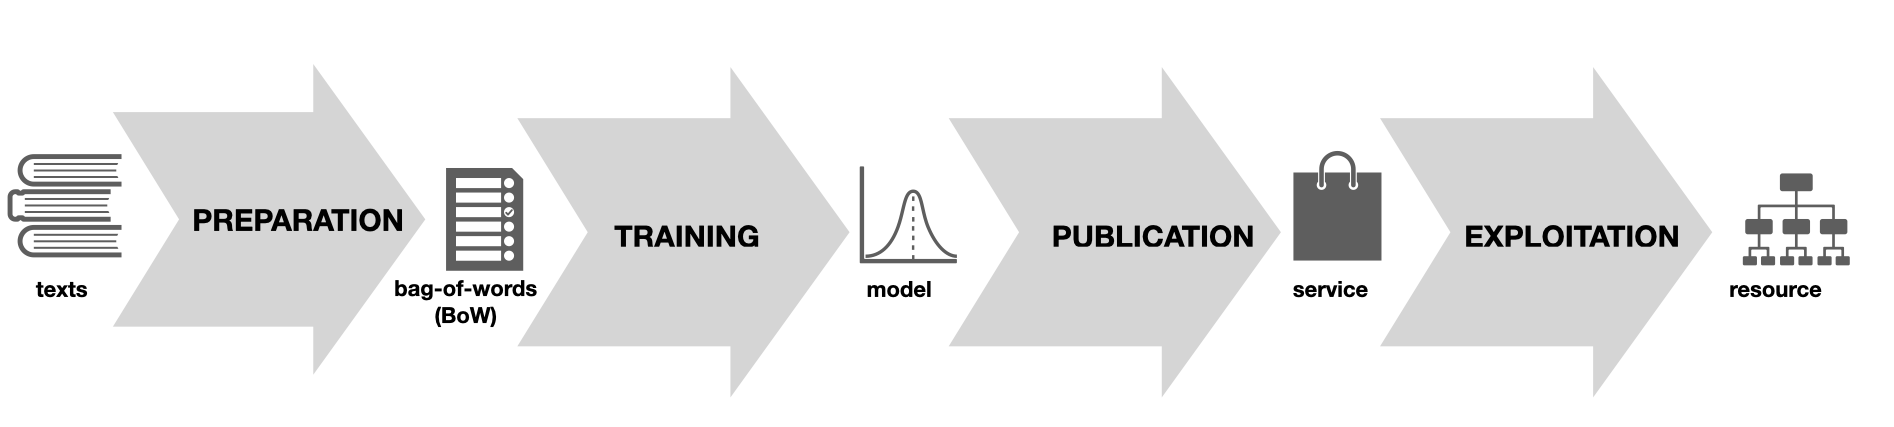
\includegraphics[scale=0.21]{life-cycle.png}
  \caption{Stages in the creation and reuse of topic models. Texts are first processed to retrieve tokens and create bags-of-words (BoW). These structures are used to train a model that identifies word distributions called topics. The model is enabled to make topic inferences in unseen texts. It is published as a web service in an online repository. The service can then be (re)used as web resource, for example to categorize documents.}
  \label{fig:life-cycle}
\end{figure}


\textit{librAIry} is a framework that covers the entire topic model life-cycle by combining learning algorithms with natural language processing methods and software distribution techniques. The main objective is to \textbf{\textit{facilitate the creation of reusable probabilistic topic models by minimizing their technical dependencies}}. Methods and algorithms proposed in this thesis have been implemented and evaluated in this framework, which therefore serves as the technological basis for our research.

Our design requirements, which have guided our development process, can be organized into three categories:
\begin{itemize}
\item \textbf{Corpora representation requirements}, which tackle the modeling of document collections and its metadata. This includes texts and their related annotations.
\item \textbf{Task distribution requirements}, which refer to event management to notify changes in document collections. Coordination of this information is crucial for robust and reproducible results.  
\item \textbf{Process execution requirements}, which capture the operations involved in creating a topic model. The parallel task execution leads to the creation of models.
\end{itemize}

The rest of the section describes how we have adapted existing techniques and standards in \textit{librAIry} to address each of the requirement categories described above. An open, distributed and scalable framework has been developed whose source code is publicly available for reuse\footnote{\url{https://doi.org/10.5281/zenodo.4561156}} and which is registered in the Intellectual Property Office of Comunidad de Madrid with reference M-7342-2016.

\subsection{Corpora Representation for Topic Modeling}
\label{sec:representing-corpora}

Inspired by a Staged Event-Driven Architecture (SEDA) that exchanges messages and handles status changes, our framework is based on \textit{resources} and \textit{actions}. A \textit{resource} can be a \textit{document} that represents raw texts (e.g. a full-text research paper), or a \textit{snippet} of text with a logical part  (e.g. sections, summaries or even phrases grouped by their rhetoric), or a \textit{domain} that contains a dataset of texts (e.g. a conference proceedings) or even an \textit{annotation} made on them (e.g. review comments, named-entities, topics). \textit{Actions} can be executed on resources to change their status (e.g. \textit{create}, \textit{update} or \textit{delete}).

To better illustrate this model, take a sample of the research articles published at the K-CAP 2019 conference\footnote{\url{http://www.k-cap.org/2019}} (see Fig. \ref{fig:librairy-model}). A \textit{document} resource is created for each publication and contains the full text of the article. Each \textit{document} is then associated with several \textit{snippets}, one for each section of the article (e.g. abstract, introduction, conclusions, etc). Finally, a \textit{domain} is created that groups all these \textit{documents} under the same conference. This initial representation can be extended with \textit{annotations}, that can provide more detailed information at different levels (e.g. named-entities, keywords or topics).

% 
\begin{figure}
  \center
  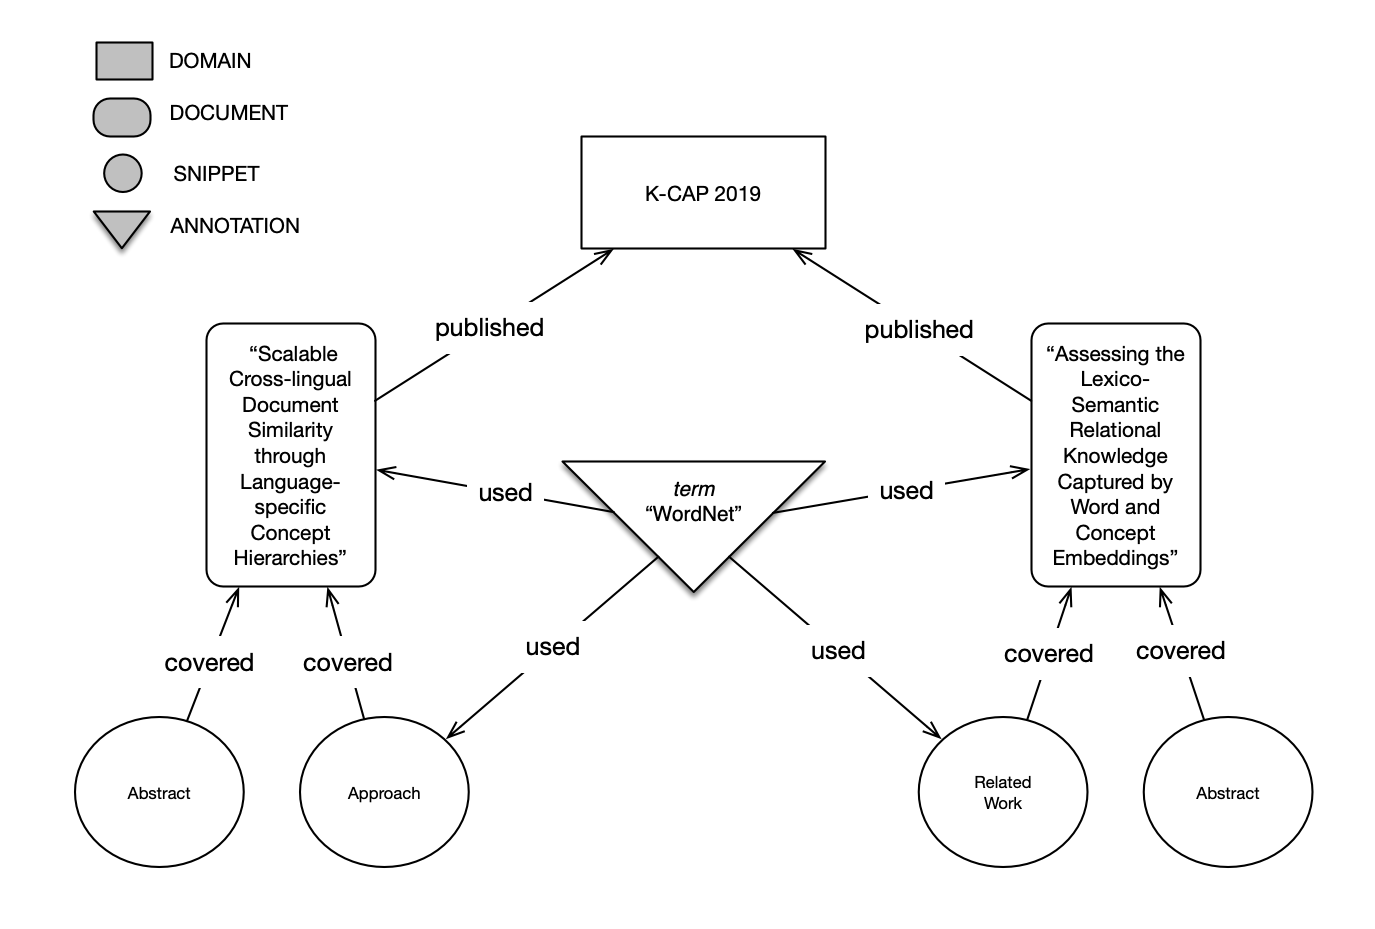
\includegraphics[scale=0.55]{model}
  \caption{Representation of two scientific papers published at the International Conference on Knowledge Capture (K-CAP, 2019) that mention the same entity, \textit{Wordnet}, in different sections.}
  \label{fig:librairy-model}
\end{figure}
% -----------

\textit{Resources} and \textit{actions} are individually addressable and linkable \citep{Turchi2012a} following Linked Data principles \citep{Bizer2009}. Each of them has: (1) a name, (2) a retrievable (or dereferenceable) HTTP URI so that it can be looked up, (3) a descriptive information provided by using standard notation (e.g. JavaScript Object Notation (JSON)) when it is  looked up by URI, and (4) links to other URIs so that other resources can be discovered from it.

More details about each of them is shown below.

\subsubsection{Domain}

A \textit{domain} is an aggregation of \textit{documents}. It is described as a group with parts separately described. Every \textit{document} that is processed belongs, at least, to one \textit{domain} (Fig \ref{fig:librairy-model-domain}).

A \textit{domain} contains the following information: 
\begin{itemize}
\item \textbf{uri}: identifier created from the resource type (i.e \textit{domains}) and a Universally Unique Identifer (UUID) (e.g \textit{domains/88b86fa6-11c8-11eb-adc1-0242ac120002})
\item \textbf{creation-time}: date when resource was created. It follows the ISO-8601\footnote{\url{https://www.iso.org/standard/40874.html}}.
\item \textbf{name}: label associated to the resource.
\item \textbf{description}: additional information about it.
\end{itemize}

\begin{figure}
  \center
  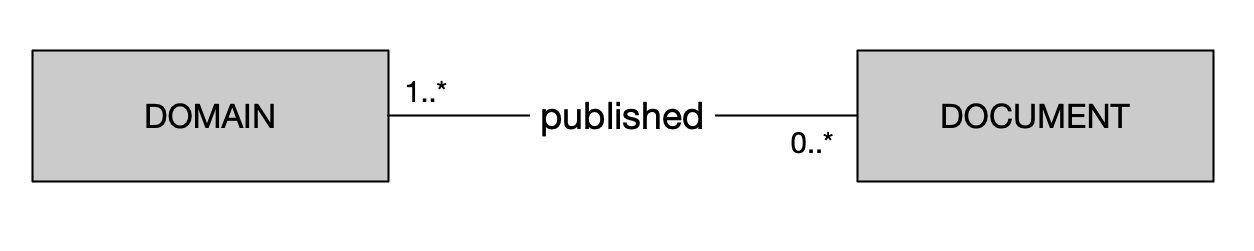
\includegraphics[scale=0.45]{model-domain.png}
  \caption{Relation between \textit{domain} and \textit{document}.}
  \label{fig:librairy-model-domain}
\end{figure}

\subsubsection{Document}

A \textit{document} is a resource consisting primarily of text. Examples include research papers, articles, books or patents. It follows the Open Archives Initiative for Object Reuse and Exchange\footnote{\url{http://www.openarchives.org}} (OAI-ORE) and the Dublin Core Metadata Initiative\footnote{\url{http://dublincore.org}} (DCMI). 

A \textit{document} contains the following information:                                                              

\begin{itemize}
\item \textbf{uri}: identifier created from the resource type (i.e \textit{documents}) and a UUID ( e.g \textit{documents/809af686-11c8-11eb-adc1-0242ac120002})
\item \textbf{creation-time}: date when resource was created. It follows the ISO-8601.
\item \textbf{publishedOn}: date when resource was published. It follows the ISO-8601.
\item \textbf{publishedBy}: an entity responsible for making the document available. It can be a  person, an  organization or a service. It may be different from the entity that conceptually formed the resource (e.g. wrote the document), which is recorded as \textit{authoredBy}. This entity should be identified by a valid Uniform Resource  Identificator (URI) such as WebId\footnote{\url{http://www.w3.org/wiki/WebID}}, orcid\footnote{\url{http://orcid.org}} or internal URI. 
\item \textbf{authoredOn}: the time the \textit{document} was conceptually formed. The author time should be present if different from \textit{publishedOn}. It must be a formatted timestamp following ISO-8601.
\item \textbf{authoredBy}: an entity primarily responsible for making the content of the \textit{document}. It may be a list to indicate multiple authors. Each of them identified by a valid URI such as WebId, orcid or internal URI.
\item \textbf{retrievedFrom}: a URI identifying the repository or source from which the document was derived. This property should be accompanied with \textit{retrievedOn}.
\item \textbf{retrievedOn}: the time the \textit{document} was retrieved on. If this property is present, the \textit{retrievedFrom} must also be present. It must be a formatted timestamp following ISO-8601.
\item \textbf{format}: the physical or digital manifestation of the resource. Typically, it includes the media-type (i.e the IANA code\footnote{\url{http://www.iana.org}}) of the \textit{document}.
\item \textbf{language}: the language(s) in which the document was written. It is defined by RFC-1766\footnote{\url{http://www.ietf.org/rfc/rfc1766.txt}} with a two-letter language code followed, optionally, by a two-letter country code.
\item \textbf{title}: a name given to the \textit{document}. It is a name by which the \textit{document} is formally known.
\item \textbf{description}: it may include but is not limited to an abstract, or a free-text account of the content.
\item \textbf{rights}: information about rights helds in and over the \textit{document}.
\item \textbf{content}: raw text from the \textit{document}.
\end{itemize}

Furthermore, a \textit{document} may contain zero or more \textit{snippets} and a \textit{snippet} may belong to one or more \textit{documents}. Since \textit{librAIry} can also discover relations among \textit{documents}, a \textit{document} may contain zero or more references to other \textit{documents} (Fig. \ref{fig:librairy-model-document}).

\begin{figure}
  \center
  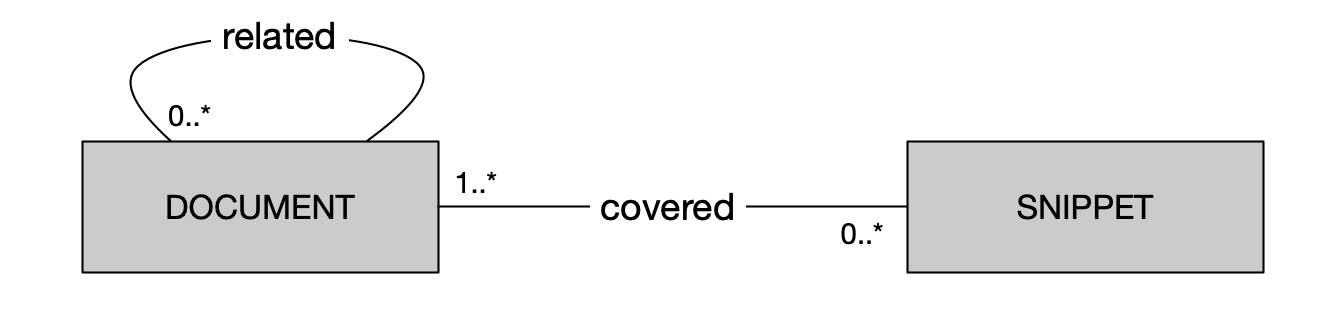
\includegraphics[scale=0.45]{model-document.png}
  \caption{Relation between \textit{document} and \textit{snippet}.}
  \label{fig:librairy-model-document}
\end{figure}

\subsubsection{Snippet}

A \textit{snippet} is a resource that is included either physically or logically in a \textit{document}. In a scientific \textit{document}, for example, it may be the \textit{abstract} section or a logical set of sentences sharing the same rhethorical class (e.g. approach, background, related-work, etc). As seen above (Fig. \ref{fig:librairy-model-document}), a \textit{snippet} can belong to one or more \textit{documents}.

It contains the following information:
\begin{itemize}
\item \textbf{uri}: identifier created from the resource type (i.e \textit{snippets}) and a UUID ( e.g \textit{snippets/7a5a46c8-11c8-11eb-adc1-0242ac120002})
\item \textbf{creation-time}: date when resource was created. It follows the ISO-8601.
\item \textbf{sense}: content-type. It refers to a section or any other criteria under which the following text makes sense (e.g. introduction, summary, notes, etc).
\item \textbf{content}: partial text retrieved from the full-text of a \textit{document}.
\end{itemize}

\subsubsection{Annotation}

\textit{Annotations} are data retrieved from resources that can be used to relate them. They are basically key-value data structures associated to \textit{domains}, \textit{documents} or \textit{snippets}. Examples are entities mentioned in a text, or topics covered in a collection. Any resource can have zero or multiple annotations, which can be shared among several resources (Fig. \ref{fig:librairy-model-annotation})

It contains the following information:
\begin{itemize}
\item \textbf{uri}: identifier created from the resource type (i.e \textit{annotations}) and a UUID ( e.g \textit{annotations/73671e68-11c8-11eb-adc1-0242ac120002})
\item \textbf{creation-time}: date when resource was created. It follows the ISO-8601.
\item \textbf{key}: a category or type associated with the information it contains (e.g. entity, comment, topic, keywords, etc). Recommended best practice is to use a controlled vocabulary.
\item \textbf{value}: a note about the resource in the form of free text.
\end{itemize}

\begin{figure}
  \center
  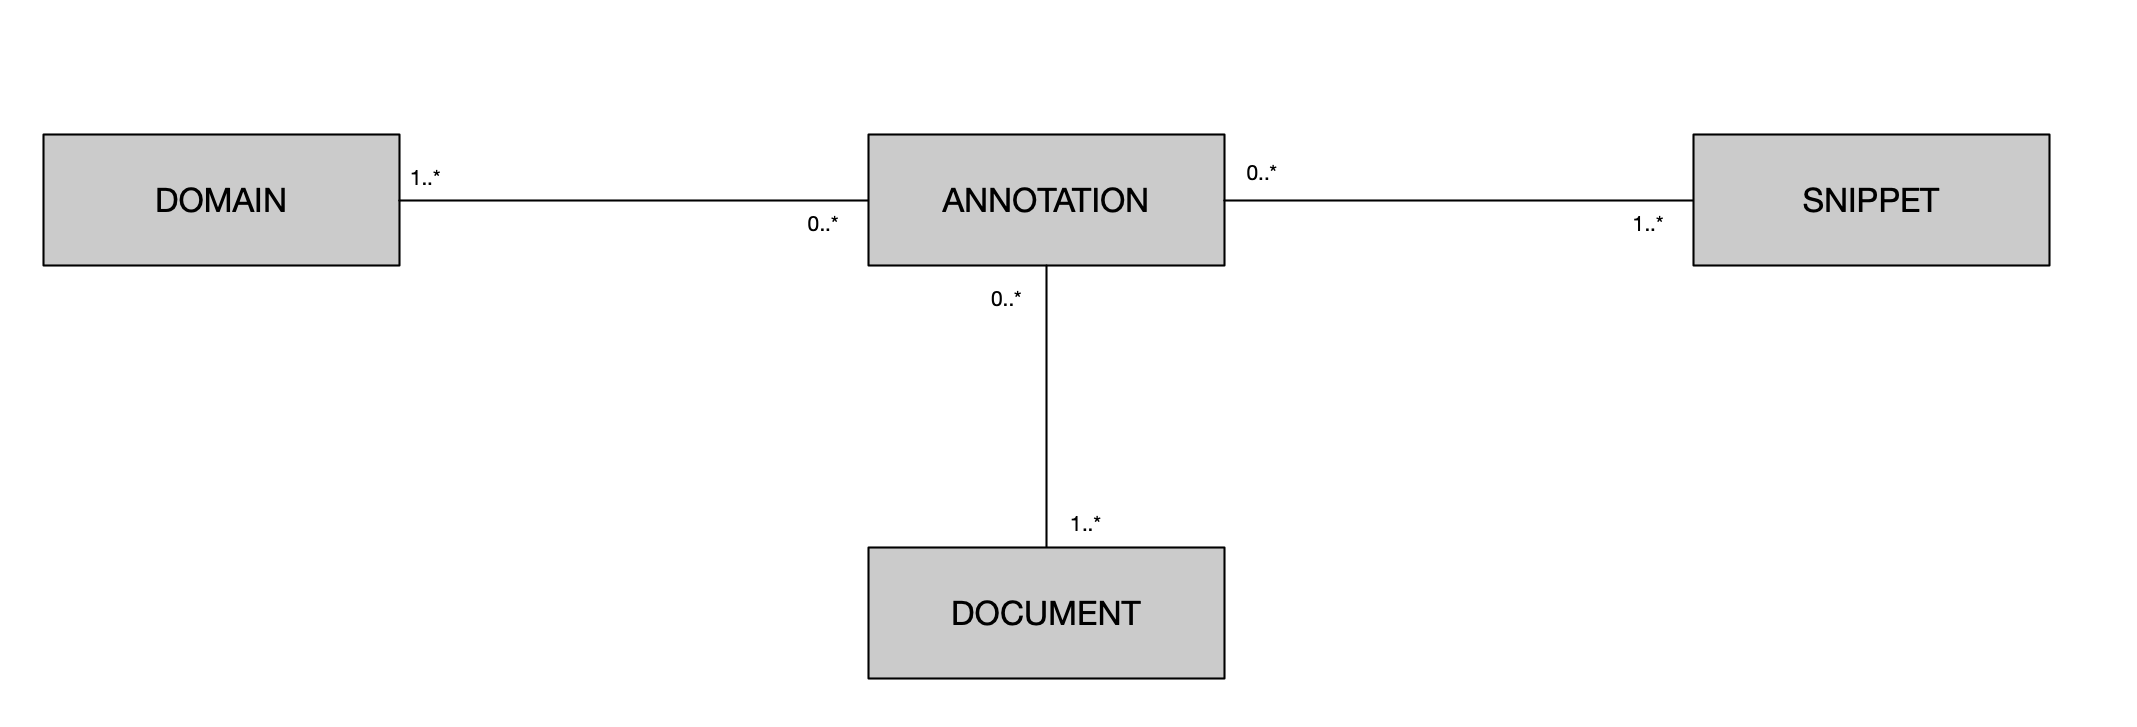
\includegraphics[scale=0.4]{model-annotation.png}
  \caption{Relation between \textit{annotations} and other resources.}
  \label{fig:librairy-model-annotation}
\end{figure}

\subsection{Event-oriented Processing Workflow}

Along with the resources mentioned above, there are two additional elements that provide a crucial behavior to the framework: \textit{modules} and \textit{events}. An \textit{event} is a non-persistent time-based occurrence that describes a new action performed on a resource. \textit{Modules} are responsible for carrying out operations on the resources (e.g. tokenize a \textit{document} or create a topic model from a \textit{domain}). \textit{Events} are broadcasted so that any \textit{module} is aware of the changes made to the resources and  can perform actions on one or more resources in response to a new state reached by a given resource. These actions are paralleled since modules are replicated through distributed environments.

%\begin{figure}
%  \center
%  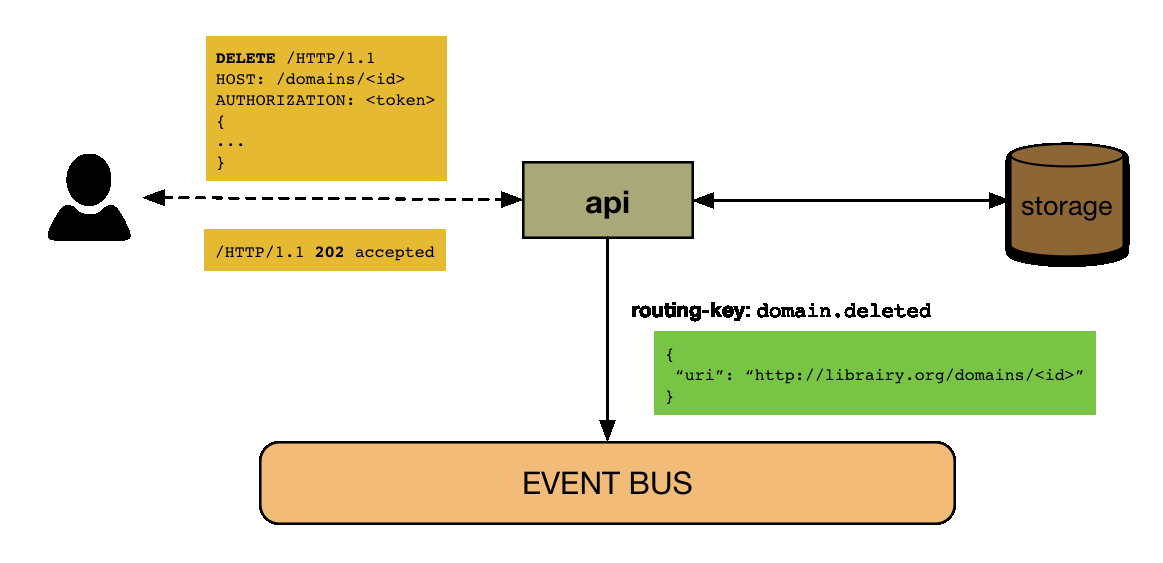
\includegraphics[scale=0.45]{api-domain-deleted}
%  \caption{Domain deleted flow.}
%  \label{fig:librairy-domain-deleted}
%\end{figure}


The framework follows a publisher/subscriber approach where \textit{modules} can publish and read \textit{events} to notify and to be notified about the state of a \textit{resource} (Fig. \ref{fig:librairy-states}). An \textit{event} notifies a performed \textit{action} (i.e. a resource and its new state), and follows the Representational State Transfer (REST) paradigm \citep{Fielding2002}. It contains the resource type and the new state reached by a specific resource ( i.e \textit{created}, \textit{deleted} or \textit{updated}). For example, when a new \textit{domain} is created, an \textit{event} message is published to the channel: $domain.created$. A channel is a space where \textit{events} are published and \textit{modules} can be subscribed to read only some \textit{events}. The actions performed by a module depend on the events to which it is subscribed. Therefore, the workflow of the framework is neither static nor explicitly defined. A distributed dynamic workflow emerges according to the \textit{modules} subscribed to the \textit{event} channels.

From a technical point of view, \textit{librAIry} uses the Advanced Message Queuing Protocol (AMQP) as the messaging standard to avoid any technical dependency to the message broker (i.e the server that sends and receives messages). This protocol defines: \textit{exchanges}, \textit{queues}, \textit{routing-keys} and \textit{binding-keys} to communicate publishers (i.e message senders) and consumers (i.e message readers). \textit{Exchanges} are like message inboxes, and \textit{queues} are subscribed to them by specifying the message types they are interested in with a \textit{binding-key}. A message sent by a publisher to an exchange is routed with a \textit{routing-key} and consumers matching that \textit{routing-key} with their \textit{binding-key} (used to connect the \textit{queue} to that \textit{exchange}), will receive the message. This mechanism allows sending and receiving messages between consumers and producers by means of shared keys (i.e. \textit{routing-keys} and \textit{binding-keys}). A key follows the structure: \textit{resource.status}. Since a wildcard-based definition can be used to set the key, this paradigm allow modules both listening to individual type events (e.g. \textit{domains.created} for new \textit{domains}), or multiple type events (e.g. \textit{\#.created} for all new resources).


\begin{figure}
  \center
  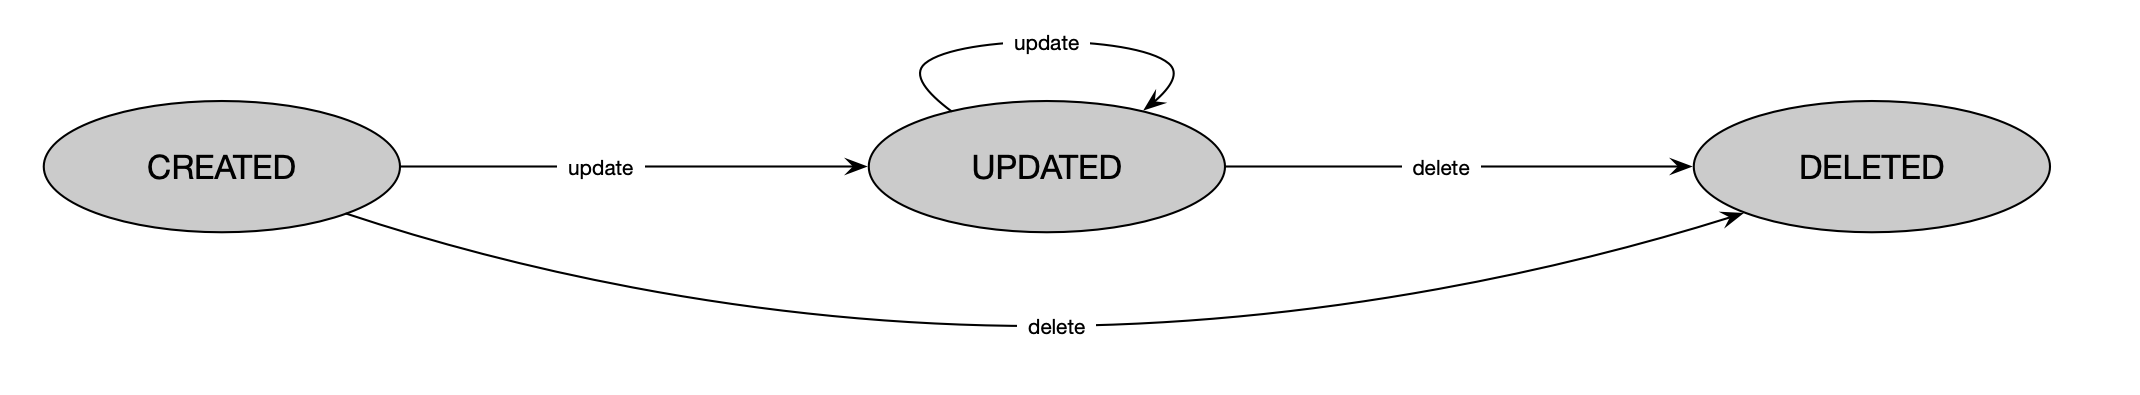
\includegraphics[scale=0.3]{resource-states.png}
  \caption{Resource states.}
  \label{fig:librairy-states}
\end{figure}


\subsection{Module-based Model Training}
\label{sec:librairy-modules}

A microservice-oriented style has been used to define the framework architecture. Using multiple services, the system analyzes texts, creates probabilistic topic models, publishes them as new services and uses them to annotate texts. A service is equivalent to a functionality, and each functionality is materialized by a \textit{module} in the system. A \textit{module} is then a cohesive and independent process \citep{Dragoni2016} with a specific purpose (i.e functionality) based on the \textit{events} to which it responds. These \textit{events} correspond to the routing- and binding- keys attached to the module.

\begin{figure} 
  \center
  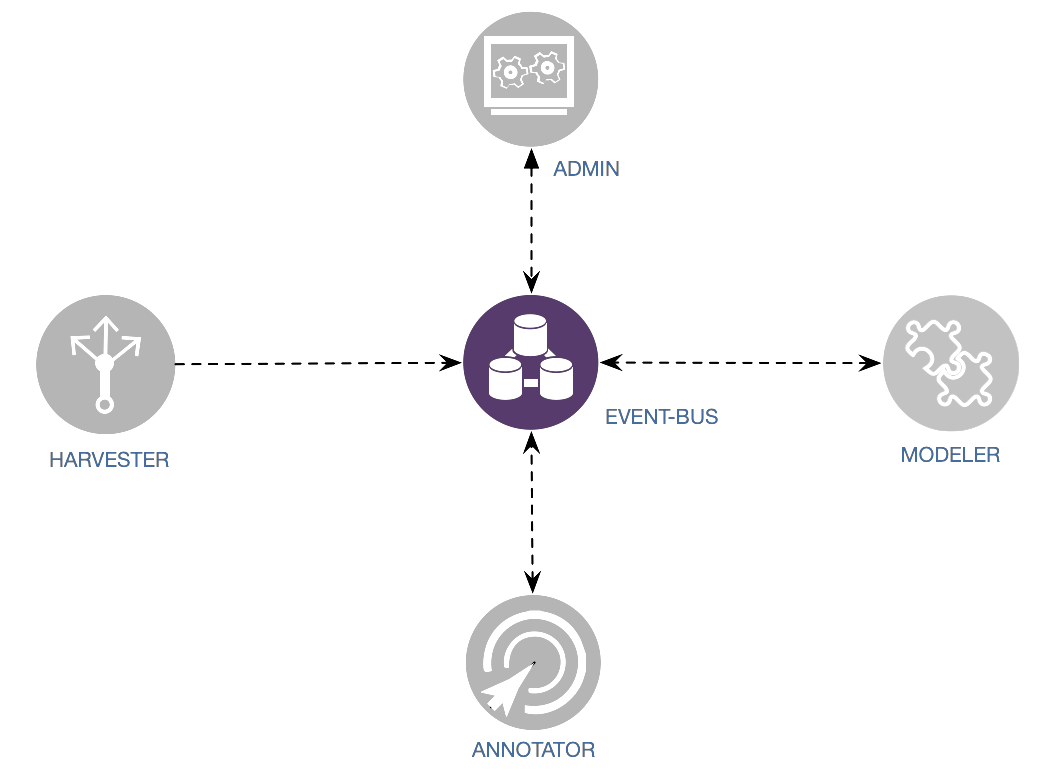
\includegraphics[scale=0.45]{modulesBN}
  \caption{Modules (in gray) publishing or receiving events from the messenger service (in purple).}
  \label{fig:librairy-modules}
\end{figure}


There are four types of \textit{modules} (Fig. \ref{fig:librairy-modules}):
\begin{itemize}
	\item \textbf{Harvester}: creates resources such as \textit{documents}, \textit{snippets} and \textit{domains}, from local or remote repositories with textual files. We have developed harvesters to create scientific resources from Elsevier\footnote{\url{https://github.com/librairy/harvester-elsevier}} or any other digital repository\footnote{\url{https://github.com/librairy/harvester-research}} that follows the Open Archives Initiative Protocol for Metadata Harvesting (OAI-PMH)\footnote{\url{https://github.com/cbadenes/camel-oaipmh}}; as well as more general ones to retrieve public datasets from datos.gob.es\footnote{\url{https://github.com/librairy/harvester-datosGobEs}} or resources located on local folders\footnote{\url{https://github.com/librairy/harvester}}.
    \begin{itemize}
    		\item \textbf{\textit{binding-queue}} (i.e listening for): nothing
		\item \textbf{\textit{routing-key}} (i.e publishing to): \textit{document.created}, \\ \textit{snippet.created}, \textit{domain.(created;updated)}
    \end{itemize}
    \item \textbf{Annotator}: creates \textit{annotations} (e.g named-entities, bag-of-words, topic distributions, etc) in \textit{documents}, \textit{snippets} or \textit{domains}. We have developed an NLP Annotator\footnote{\url{http://librairy.linkeddata.es/nlp}} that creates bag-of-words from a given text by normalizing its content through natural language processing tasks such as named entity recognition, lemmatization or part-of-speech (PoS) tagging. The source code\footnote{\url{https://github.com/librairy/nlp}} is publicly available for reuse. Topic models are also annotators in this framework, as will be seen in section \ref{sec:topic-model-publication}.
    \begin{itemize}
    	\item \textbf{\textit{binding-key}}: \textit{document.(created;updated)}, \textit{snippet.(created;updated)}
	\item \textbf{\textit{routing-key}}: \textit{annotation.(created;deleted)}
    \end{itemize}
    \item \textbf{Modeler}: creates probabilistic topic models for \textit{domains} from the bag-of-word \textit{annotations} of each \textit{document}. We have developed a LDA Modeler\footnote{\url{https://github.com/librairy/modelerTopics-service}} as well as a W2V Modeler\footnote{\url{https://github.com/librairy/modeler-w2v}} (the latter for testing purposes). 
    \begin{itemize}
    	\item \textbf{\textit{binding-key}}: \textit{domain.(created;updated)}, \textit{annotation.created}
	\item \textbf{\textit{routing-key}}: \textit{annotation.(created;deleted)}	
	\end{itemize}
	\item \textbf{Administrator}: performs user-driven tasks such as reading/writing/updating resources or database queries. As with the other modules, the source code\footnote{\url{https://github.com/librairy/api}} is publicly available for reuse. Together with the API, we have also developed a web interface\footnote{\url{https://github.com/librairy/explorer}} to visualize documents, their relationships and the topics associated with each \textit{domain}. 	
    \begin{itemize}
    	\item \textbf{\textit{binding-key}}: \textit{\#.\#}
	\item \textbf{\textit{routing-key}}: \textit{domain.(created;updated;deleted)}, \\ \textit{document.(created;updated;deleted)}, \textit{snippet.(created;updated;deleted)}, \\ \textit{annotation.(created;updated;deleted)}
    \end{itemize}
\end{itemize}


Figure \ref{fig:librairy-sequence} shows a sequence diagram that illustrates how modules work collaboratively to create a topic model from documents added to the framework. Each module provides an Application Program Interface (API) over HTTP, that follows the web standards for the RESTful API development, and a Avro\footnote{\url{https://avro.apache.org}}-based interface over TCP for efficiency reasons. Among them the communication is done over TCP.  

\begin{figure} 
  \center
  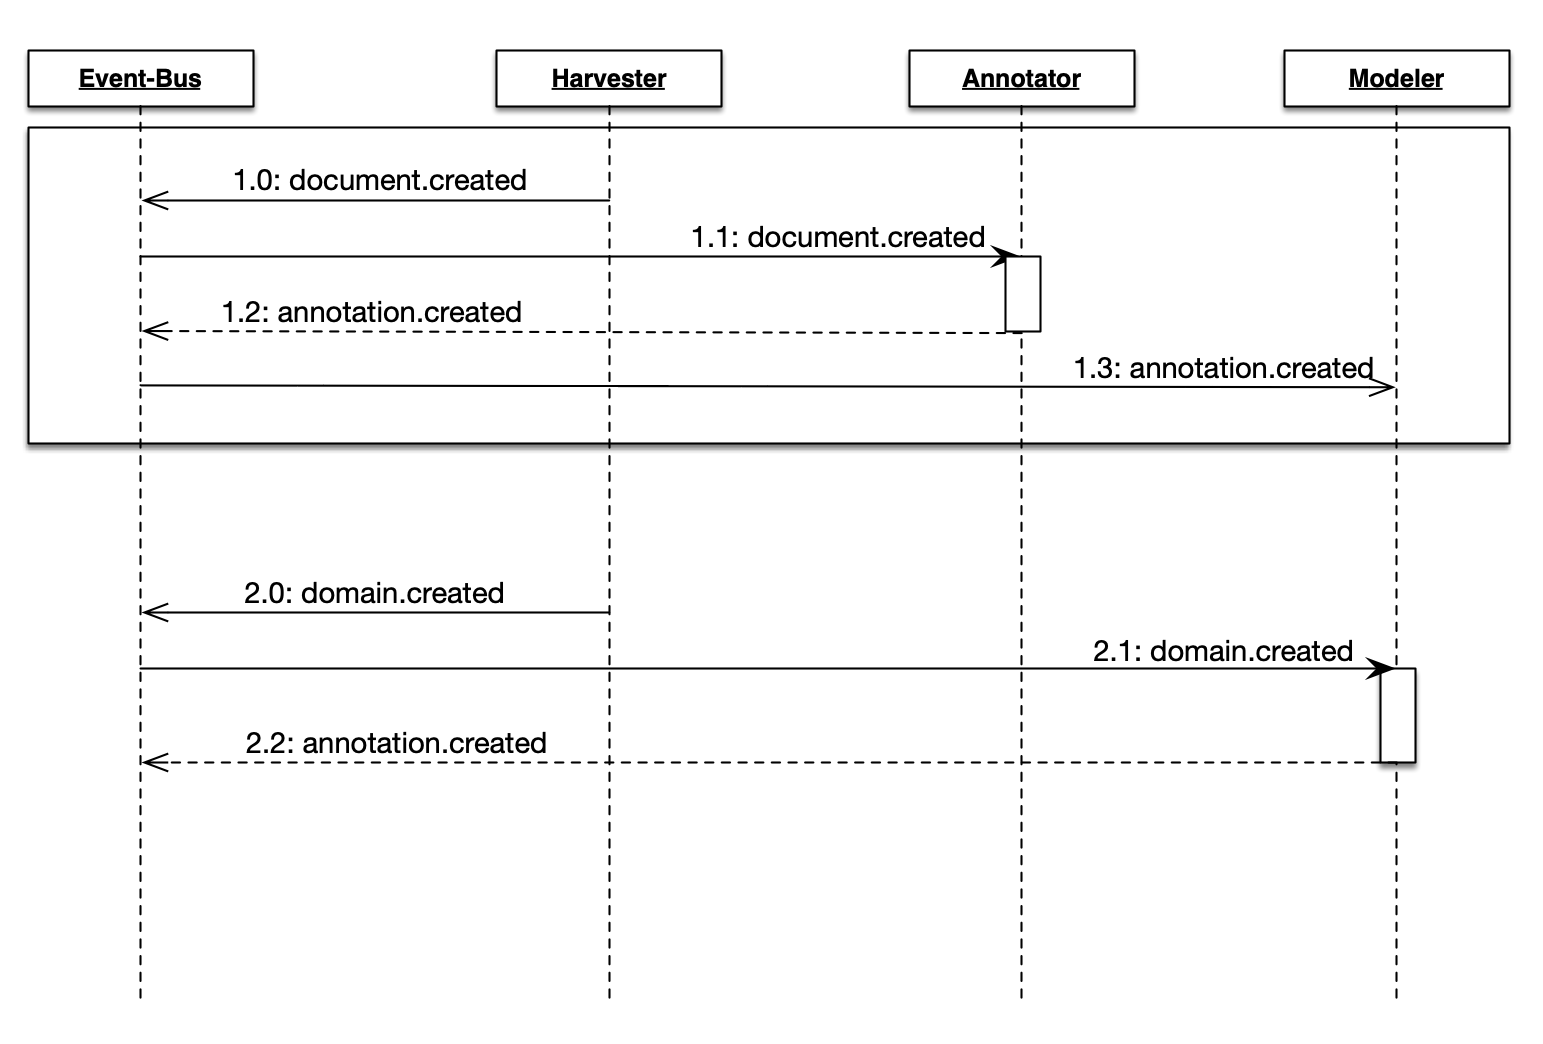
\includegraphics[scale=0.45]{librairy-sequence.png}
  \caption{Sequence of \textit{events} exchanged between modules to create a topic model from the \textit{documents} added to a \textit{domain}.}
  \label{fig:librairy-sequence}
\end{figure}




\section{Topic Modeling Services}
\label{sec:reusable-topic-modeling}

In order to use an existing topic model in our framework, which is micro-services-oriented, the model itself needs to be a service. This approach decouples the resources used to train a probabilistic topic model (e.g. data format or algorithm implementation), from the resources required to  make inferences and thus avoids unexpected incompatibilities. In this way, we simultaneously facilitate the reuse of topic models and also their scalable execution.

\subsection{Topic Model Publication}
\label{sec:topic-model-publication}

We propose distributing topic models as services hosted in online repositories. Models are packaged as OS-level virtualization software that can run reliably applications from one computing environment to another. A model becomes a standalone and executable software package that includes everything needed to use it: code, data, runtime libraries, system tools and settings.

There are several technologies that can virtualize services. Among them, Docker\footnote{\url{https://www.docker.com/}} stands out as a de facto standard due to its wide adoption. It is a platform as a service (PaaS) environment that use operating service-level virtualization to deliver software in packages called \textit{containers}. Containers are isolated from one another and bundle their own software, libraries and configuration files. All containers are run by a single operating system kernel and therefore use fewer resources than virtual machines.

Topic Models in \textit{librAIry} are packaged as Docker \textit{containers} and published in online repositories\footnote{\url{https://hub.docker.com/repositories}} so they can be easily downloaded and run on any machine or software solution. Containers do not only offer virtualization advantages, but also version and license control, since they handle some information that we use to characterize our models:
\begin{itemize}
\item \textbf{repository}: model name (e.g. dbpedia-model).
\item \textbf{author}: model creator (e.g. librAIry)
\item \textbf{version}: model version (e.g. 3.0)
\item \textbf{license}: model license (e.g. Apache 2.0)
\end{itemize}


\subsection{Topic Model Exploitation}
\label{sec:topic-model-exploitation}

Once a topic model has been packaged as a virtual service (i.e. Docker containers), either assembled as a \textit{annotator} in librAIry or as an online service accessible via its HTTP (based on a OpenAPI interface, Fig. \ref{fig:librairy-topic-model-swagger}) or TCP (based on an Avro\footnote{\url{https://github.com/librairy/modeler-service-facade/blob/master/src/main/avro/model.avpr}} interface) API, it should support all tasks that can be performed on a topic model. Taking into account the \textbf{\textit{reproducibility}} of a model, the \textit{conditions under which the model has been created}, in relation to the corpus (i.e. number of documents, vocabulary size, language,.. ), about NLP tasks (i.e stopwords, PoS filtering) and about the model itself (i.e. hyperparameters) should be collected and provided by the service. Taking into account the \textbf{\textit{exploration}} of a model, the \textit{topics and their word distributions} must also be available. The word distribution is usually omitted when publishing topic models providing only the top10 or top5 words per topic. This limits the capacity of the model to be exploited in tasks where that information is required, for example this thesis (as will be seen in chapter 4). And finally, taking into account the topic \textbf{\textit{inference}} in new texts, which is the most extended ability of these models, the service must be able to calculate topic distributions from texts.

\begin{figure} 
  \center
  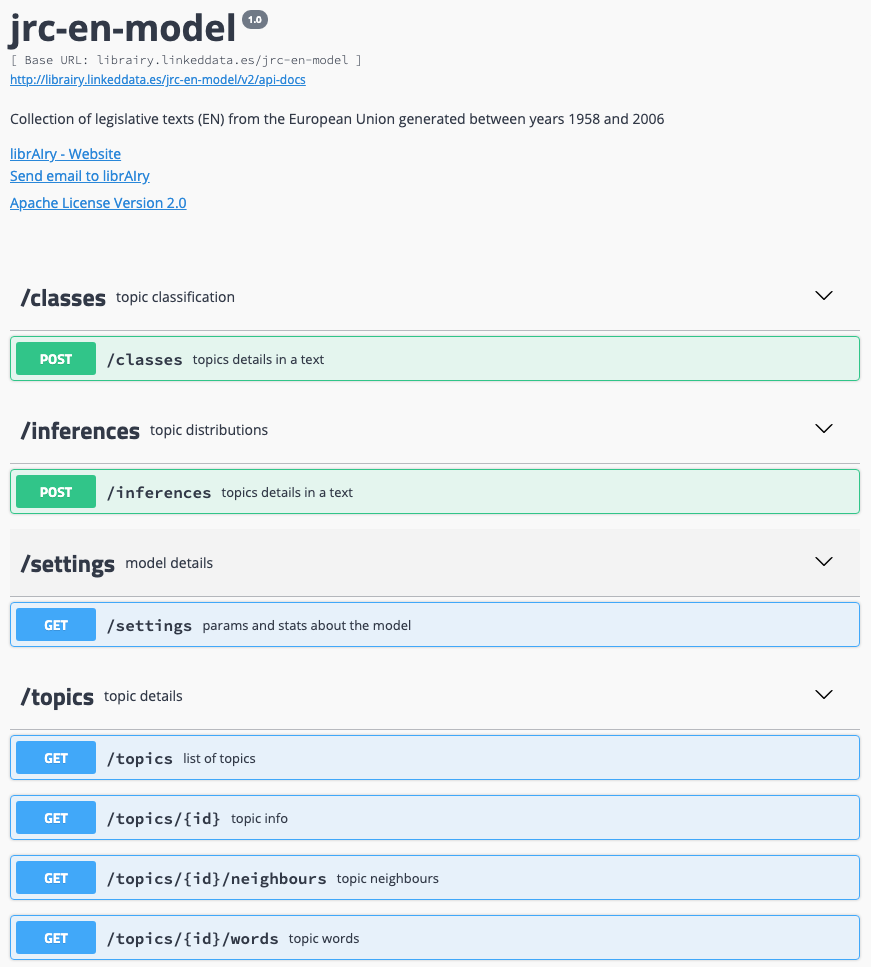
\includegraphics[scale=0.45]{topic-model-swagger.png}
  \caption{OpenAPI-based web interface of a probabilistic topic model service created with \textit{librAIry}.}
  \label{fig:librairy-topic-model-swagger}
\end{figure}


A summary of the tasks, and their purposes, provided by a topic model can be found in Table~\ref{table:tasks}. 

\begin{table}[!htbp]
\centering%
\begin{tabularx}{\linewidth}{bs}
\toprule
\heading{Task} & \heading{Purpose} \\
\midrule
\midrule
T1: Replication & create similar topics\\
\midrule
T2: Exploration & browse topics and words\\
\midrule
T3: Inference & calculate topic distributions\\
\bottomrule
\end{tabularx}
\caption{Potential uses of a topic model.}
\label{table:tasks}
\end{table}

In order to cover these tasks by topic services, the API must offer operations that, individually or partially, allow them to be achieved. A topic model is: \textit{reproducible} (T1) when its hyperparameters and the configuration of the training set are known, \textit{explorable} (T2) when the word distributions of each topic are known, and is \textit{interpretable} (T3) when the presence of each topic can be measured in a text. Table~\ref{table:operations} summarizes the operations offered by a topic model-as-a-service to support the potential uses.

\begin{table}[!htbp]
\small
\centering%
\begin{tabularx}{\linewidth}{bb}
\toprule
\heading{Operations} & \heading{Tasks} \\
\midrule
\midrule
O1: reading of model hyperparameters (i.e alpha, beta, and number of topics) & T1: Replication\\
\midrule
O2: reading of pre-processing tasks (i.e stopwords, normalization, PoS filtering) & T1: Replication\\
\midrule
O3: reading of learning parameters (i.e iterations, seed, likelihood) & T1: Replication \\
\midrule
O4: reading of topics described by word distributions (i.e topic relevance) & T2: Exploration\\
\midrule
O5: reading of words described by topic distributions (i.e word relevance) & T2: Exploration\\
\midrule
O6: calculation of topic distributions in texts (i.e vector of topic distributions) & T3: Inference\\
\bottomrule
\end{tabularx}
\caption{Operations offered by a topic model-as-a-service to cover potential tasks.}
\label{table:operations}
\end{table}

The rest of the section describes how the model implements these operations through service methods. A topic model-as-a-service is online available for review\footnote{\url{http://librairy.linkeddata.es/jrc-en-model}}.

\subsubsection{Reproducibility Tasks}
Through a single request to the model API, a list of parameters is provided to support the O1, O2, and O3 operations. The method is available by both a HTTP-GET request on \textit{\url{/settings}} resource and by a TCP request on \textit{getSettings} method. An online example is available here\footnote{\url{http://librairy.linkeddata.es/jrc-en-model/settings}}. 

A detailed list of the parameters provided by the topic model is shown below:
\begin{itemize}
\item \textbf{algorithm}: method used to train the model (e.g. LDA).
\item \textbf{date}: when the model was created. It follows the ISO-8601.
\item \textbf{params}: configuration of the learning process.
	\begin{itemize}
	\item \textbf{seed}: numerical value to ensure consistent results (e.g. 1066).
	\item \textbf{lowercase}: if true, text is converted to lowercase.
	\item \textbf{topics}: number of topics.
	\item \textbf{language}: language of texts.
	\item \textbf{iterations}: number of sampling iterations.
	\item \textbf{entities}: if true, NER tasks are performed.
	\item \textbf{max-doc-ratio}: maximum word presence per document ratio (e.g. 0.9).
	\item \textbf{min-freq}: minimum word presence per number of document (e.g. 5). 
	\item \textbf{alpha}: prior distribution over topic weights in each document (e.g. 0.1)
	\item \textbf{beta}: prior distribution over word weights in each topic (e.g. 0.01)
	\item \textbf{part-of-speech}: word classes used in the model (e.g. NOUN, VERB, ADJECTIVE)
	\item \textbf{top-words}: number of words used to describe a topic (e.g. 10)
	\item \textbf{stop-words}: list of words removed from the corpus (e.g. quantity, datum) 
	\end{itemize}
\item \textbf{stats}: statistics after the learning process.
	\begin{itemize}
	\item \textbf{loglikelihood}: how much the model fits with the training set.
	\item \textbf{vocabulary}: number of unique words.
	\item \textbf{topic-coherence}: distance between topics from their top words (e.g min, max, mean, mode).
	\item \textbf{topic-distance}: distance between topics from their word distributions (e.g min, max, mean, mode).
	\item \textbf{corpus}: number of documents in the training set. 
	\end{itemize}
\end{itemize}


\subsubsection{Exploration Tasks}
The exploration task, with its respective operations of reading topics (O4) and words (O5), is broken down into four services:

\begin{itemize}
\item \textbf{Topic List}(O4). By means of the HTTP-GET \textit{/topics}\footnote{\url{http://librairy.linkeddata.es/jrc-en-model/topics}} resource and the TCP \textit{getTopics} method, all the topics of the model are listed. Each topic is described with an increasing unique \textit{identifier} (from 0 to the maximum number of topics), a label or \textit{name} in case it has been established, and a \textit{description} with the most relevant words (based on their density distributions). 
\item \textbf{Topic Detail}(O4). By means of the HTTP-GET \textit{\url{/topics/_id_}}\footnote{\url{http://librairy.linkeddata.es/jrc-en-model/topics/0}} resource and the TCP \textit{getTopic} method, a topic identified by \textit{id} is described by providing its \textit{identifier}, \textit{name}, \textit{description} and \textit{entropy} (i.e how different is with respect the other topics).
\item \textbf{Topic Words}(O5). By means of the HTTP-GET \textit{\url{/topics/_id_/words}}\footnote{\url{http://librairy.linkeddata.es/jrc-en-model/topics/0/words}} resource and the TCP \textit{getTopicWords} method, a list of word distributions for the topic identified by \textit{id} is provided. Every word has its weight (i.e relevance score) with respect to the topic.
\item \textbf{Topic Neighbours}(O4). By means of the HTTP-GET \textit{\url{/topics/_id_/neighbours}}\footnote{\url{http://librairy.linkeddata.es/jrc-en-model/topics/0/neighbours}} resource and the TCP \textit{getTopicNeighbours} method, a list of topics related to the topic identified by \textit{id} is provided. The distance between topics is measured from their word distributions.  
\end{itemize}

\subsubsection{Inference Tasks}

A single request with the text to be analyzed returns a list with the presence of each topic (O5) in that text. The method is available by both a HTTP-POST request to \textit{\url{/inferences}} or a TCP request to the  \textit{createInference} method, with a JSON message containing the text  to be analyzed.

% existentes herramientas de análisis de textos: escalabilidad vertical

% en que consiste los modelos probabilísticos de tópicos para necesitar tareas de NLP


%In natural language processing, the term topic means a set of words. These are the words that come to mind when thinking of this topic. For example music could associate the words sound, instrument and composition. Without going more deep now, a topic model automatically discovers the words that are most likely to describe the topics present in a document collection. A trained model may then be used to infer which of these topics occur in new documents and can also pick out which portions of a document cover which topics.

%The learning process in a topic model first requires creating bag-of-words (BoW) from texts. A BoW contains the frequencies of each word in a text. The model uses these representations to discover the word distributions that best define the topics to fit their presences in the documents, assuming that a document can covers several topics. Take the following text: "Apple has just released in its Apple Store a video celebrating International Women's Day, about the lives of several relevant women, especially the most influential young woman in recent years.". A basic approach would transform that text into a BoW that considers whitespaces and punctuation marks as word separators (e.g. 'Apple'(2), 'has'(1), 'just'(1), etc). But this approach makes several mistakes. 'Apple' does not appear twice, but only once, as 'Apple Store' is different to 'Apple'. Some natural language processing tasks are needed to make these assessments. Using Named Entity Recognition (NER) techniques, for example,  'Apple', 'Apple Store' and 'International Women's Day' are different words in a BoW. Sometimes a normalization is applied to group plural and singular nouns. Using stemming techniques and Part-of-Speech (PoS) tagging, 'women' and 'woman' are transformed into a same word, 'woman', with a frequency equals to the sum of their frequencies, in this case 2. This is just a very simple illustration of how texts need to be processed to train probabilistic topic models. 

%While most topic model tools already include such functionality, they have not taken into account integration and scalability issues in their development. It is difficult, and sometimes impossible, to incorporate external resources into the workflow to perform some of these tasks (e.g. NER, PoS Tagging, etc) due to incompatibility problems. They can appear at the data level with different annotation categories (e.g. AnCora and CoNLL-U tagsets for PoS tagging), or at the execution level with different technological stacks (e.g. Java and Python). Furthermore, they are mainly focused on vertical scalability (better processing machines), instead of horizontal scalability (more processing machines). There are tools that have recently addressed, although only partially, some of these incompatibilities\footnote{\url{https://www.openml.org}}. But, as far as we know, these approaches keep forgetting the horizontal scalability in their designs. Only with high-performance machines can huge document collections be processed, instead of combining some lower-performance machines.

%We propose a distributed framework where multiple and heterogeneous text mining tools can collaboratively work. A shared workflow emerges to combine external tools (e.g. java-based and python-based tools to create topic models and NLP tasks), that may be located on different machines and even replicated at different scales. This raises both technical and functional challenges to coordinate distributed executions. From the technical point of view, isolated environments and communication mechanisms are required so dissimilar tools can be executed with maximum guarantees. From the functional point of view, all executions must be coordinated to reach a final result as aggregation of partial results derived from each execution.

 


%\subsubsection{Storage}

%Multiple types of data can be handled in this ecosystem. Inspired in the Data Access Object (DAO) pattern, we have created a Unified Data Manager (UDM) providing access to any type of data used in the system.  Three types of databases have been considered:
%\begin{itemize}
	%\item \textbf{column-oriented database}: Focused on unique identified and/or \textit{structured data}. This storage allow %us searching key elements across resources. 
	%\item \textbf{document-oriented database}: Focused on indexing raw text. This storage allow us to execute advanced search %operations over all the information gathered about a textual resource. 
    %\item \textbf{graph database}: Focused on relations. This storage allow us exploring resources through the relationships %between them.
%\end{itemize}


\section{Summary}

In Section \ref{sec:topic-model-framework} we have described \textit{librAIry}, the framework to cover the entire topic model life-cycle in a scalable way. Algorithms and tools coming from different technologies work collaboratively to process and analyze huge collections of textual resources creating and using probabilistic topic models. 

We tested and validated \textit{librAIry} by using the framework in some real world scenarios such as DrInventor\footnote{\url{http://drinventor.eu}}, where thousands of scientific publications were processed, TheyBuyForYou\footnote{\url{https://theybuyforyou.eu}}, where hundreds of thousands of public procurement texts were analyzed, or 
CorpusViewer\footnote{\url{https://www.plantl.gob.es/tecnologias-lenguaje/actividades/plataformas/Paginas/corpus-viewer.aspx}}, where millions of patents were automatically organized. Thus, \textit{librAIry} has proven to be a valid and scalable text processing framework and addresses the first technical objective of this thesis ( T01, \textit{create a scalable platform for  topic modeling}).

\textit{librAIry} has been designed to represent corpora by organizing the data in three levels of detail: \textit{snippets} to reflect parts or pieces of texts, \textit{documents} to represent full texts, and \textit{domains} to group documents. Transversally there are \textit{annotations}, which allow providing more details to any of them. Figure \ref{fig:librairy-model} shows how two scientific articles published in the same conference and that mention a same resource in their papers can be represented. On this representation model based on SEDA architectures, actions over resources and status change notification events are introduced, which enable to distribute the processing of resources. Figure \ref{fig:librairy-modules} shows the four modules involved in processing the resources. \textit{Harvester} modules create new \textit{documents}, \textit{snippets} and \textit{domains}. \textit{Annotator} modules react to each new resource and introduce \textit{annotations}. \textit{Modeler} modules create new topic models for each new \textit{domain}. And \textit{Admin} modules perform administrative tasks and allow users to read the data. As shown in figure \ref{fig:librairy-sequence}, modules coordinate their actions by reacting to the notifications. The actions are then executed in parallel through a distributed workflow and the first research objective of this thesis is addressed (RO1, \textit{define a distributed text-processing model for creating large probabilistic topic models}).

In Section \ref{sec:reusable-topic-modeling} we propose the publication of topic models as web services that can be used from external solutions or integrated into the \textit{librAIry} framework. Regardless of their API, since they work both over HTTP and over TCP, there are three types of tasks that guide the definition of the service: \textit{reproducibility}, \textit{exploration}, and \textit{inference}. Tables~\ref{table:tasks} and \ref{table:operations} detail the operations  supported by the service to cover these tasks. The definition of a topic model-as-a-service covers the second research objective of this thesis (R02, \textit{define a template to package probabilistic topic models as web services}).
 
And finally, in order to facilitate the reuse of the topic models published as web services, section \ref{sec:topic-model-publication} presents an online repository based on virtual services. This covers the second technical objective of the thesis (T02, \textit{create a repository of topic-based web services}). 
 
%A new model definition based on the previously mentioned principle of maximizing information re-usability and minimize irrelevant data has been studied to create a fine-grained resource design. New domains, in the sense of particular vocabularies or specific textual formats, have been also analyzed to be included into the system via specific harvesters or more precise annotators. Moreover, a template-based mechanism oriented to facilitate the integration of new tools and techniques into the system has been built to make easier to develop new modules as well as increasing the available modules in public repositories.

%Our approach to create and inference probabilistic topics is \textbf{scalable} enough to work properly in both situations. This chapter presents a framework for processing topic models in document collections ranging from only a few texts, to large scale corpora. Methods and algorithms proposed in this thesis have been implemented and evaluated in this environment, which therefore serves as the technological basis for our research. The motivation is twofold, on the one hand to create a scalable system to analyze documents and discover topics, and on the other hand to create reusable topic models that can be easily integrated into that system.


% this file is called up by thesis.tex
% content in this file will be fed into the main document

%: ----------------------- introduction file header -----------------------
\chapter{Explainable Topic-based Associations}\label{ch:explainability}

\graphicspath{{explainability/figures/}}

% -------------------------------------------------------------
% -- Explainability
% -------------------------------------------------------------

As stated in Chapter \ref{ch:hypothesis}, one of our hypotheses aims to determine whether it is possible to semantically relate texts taking into account their most relevant topics (H1.2). In particular, our goal is to determine whether two documents can be related by identifying their most representative topics.

However, as seen in Section \ref{sec:topic-explainability}, interpreting how documents are related from their topic distributions is hard when using density-based measures (e.g. distance equals to 0.74 or 0.76). The same pair of documents may vary their distance from each other when using topic models with different dimensions to represent them, as shown in figure \ref{fig:topic_distances}. High dimensional models create more specific topics than models with fewer dimensions, and this topic specificity influences the way in which topic distributions are related, and consequently how documents can be related. 

In order to better understand the relations derived from topic distributions, Section \ref{sec:topic-relations} compares scientific articles from their representations based on full-content, abstracts (i.e manual summaries), or summaries created automatically. Two types of metrics are considered: (i) \textit{internal-representativeness}, focused on describing the content, and \textit{external-representativeness}, focused on discovering relations \citep{Badenes-Olmedo2017c}.    

In Section \ref{sec:topic-clustering}, once we know how the topics are used to represent and relate texts, we propose a new topic-based annotation based only on the most representative topics, and a new distance measure that takes advantage of these representations \citep{Badenes-Olmedo2017b}. The main goal is not only to cluster texts through their most relevant topics, but also to facilitate the interpretation of their relations. 


\section{Topic-based Relations}
\label{sec:topic-relations}

This section studies the ability of topic distributions to capture the representativeness of a text through the relations that can be derived from it. In particular, it examines the performance offered by topic-based representations to describe scientific articles from their full-texts compared to representations based on summaries (e.g. \textit{abstract}). The objective is twofold, to analyze comparisons based on topic distributions on the one hand, and to identify strengths and weaknesses when using \textit{abstracts} to compare scientific articles on the other hand . Two novel measures are proposed based on the capability of the summary to substitute the original paper (Figure \ref{fig:representativeness}): (1) \textit{internal-representativeness}, which evaluates how well the summary represents the original full-text and (2) \textit{external-representativeness}, which evaluates the summary according to how the summary is able to produce a  set of related texts that are similar to what the original full-text has triggered.

Some studies \citep{Westergaard2017, Sciences2016} have shown that text mining of full research articles give consistently better results than using only their corresponding abstracts. Given the size limitations and concise nature of abstracts, they often omit descriptions or results that are considered to be less relevant but still are important in certain Information Retrieval tasks. Thus, when other researchers cite a particular paper, 20\% of the keywords that they mention are not present in the abstract \citep{Divoli2012}.

\begin{figure}[!htbp]
\centering
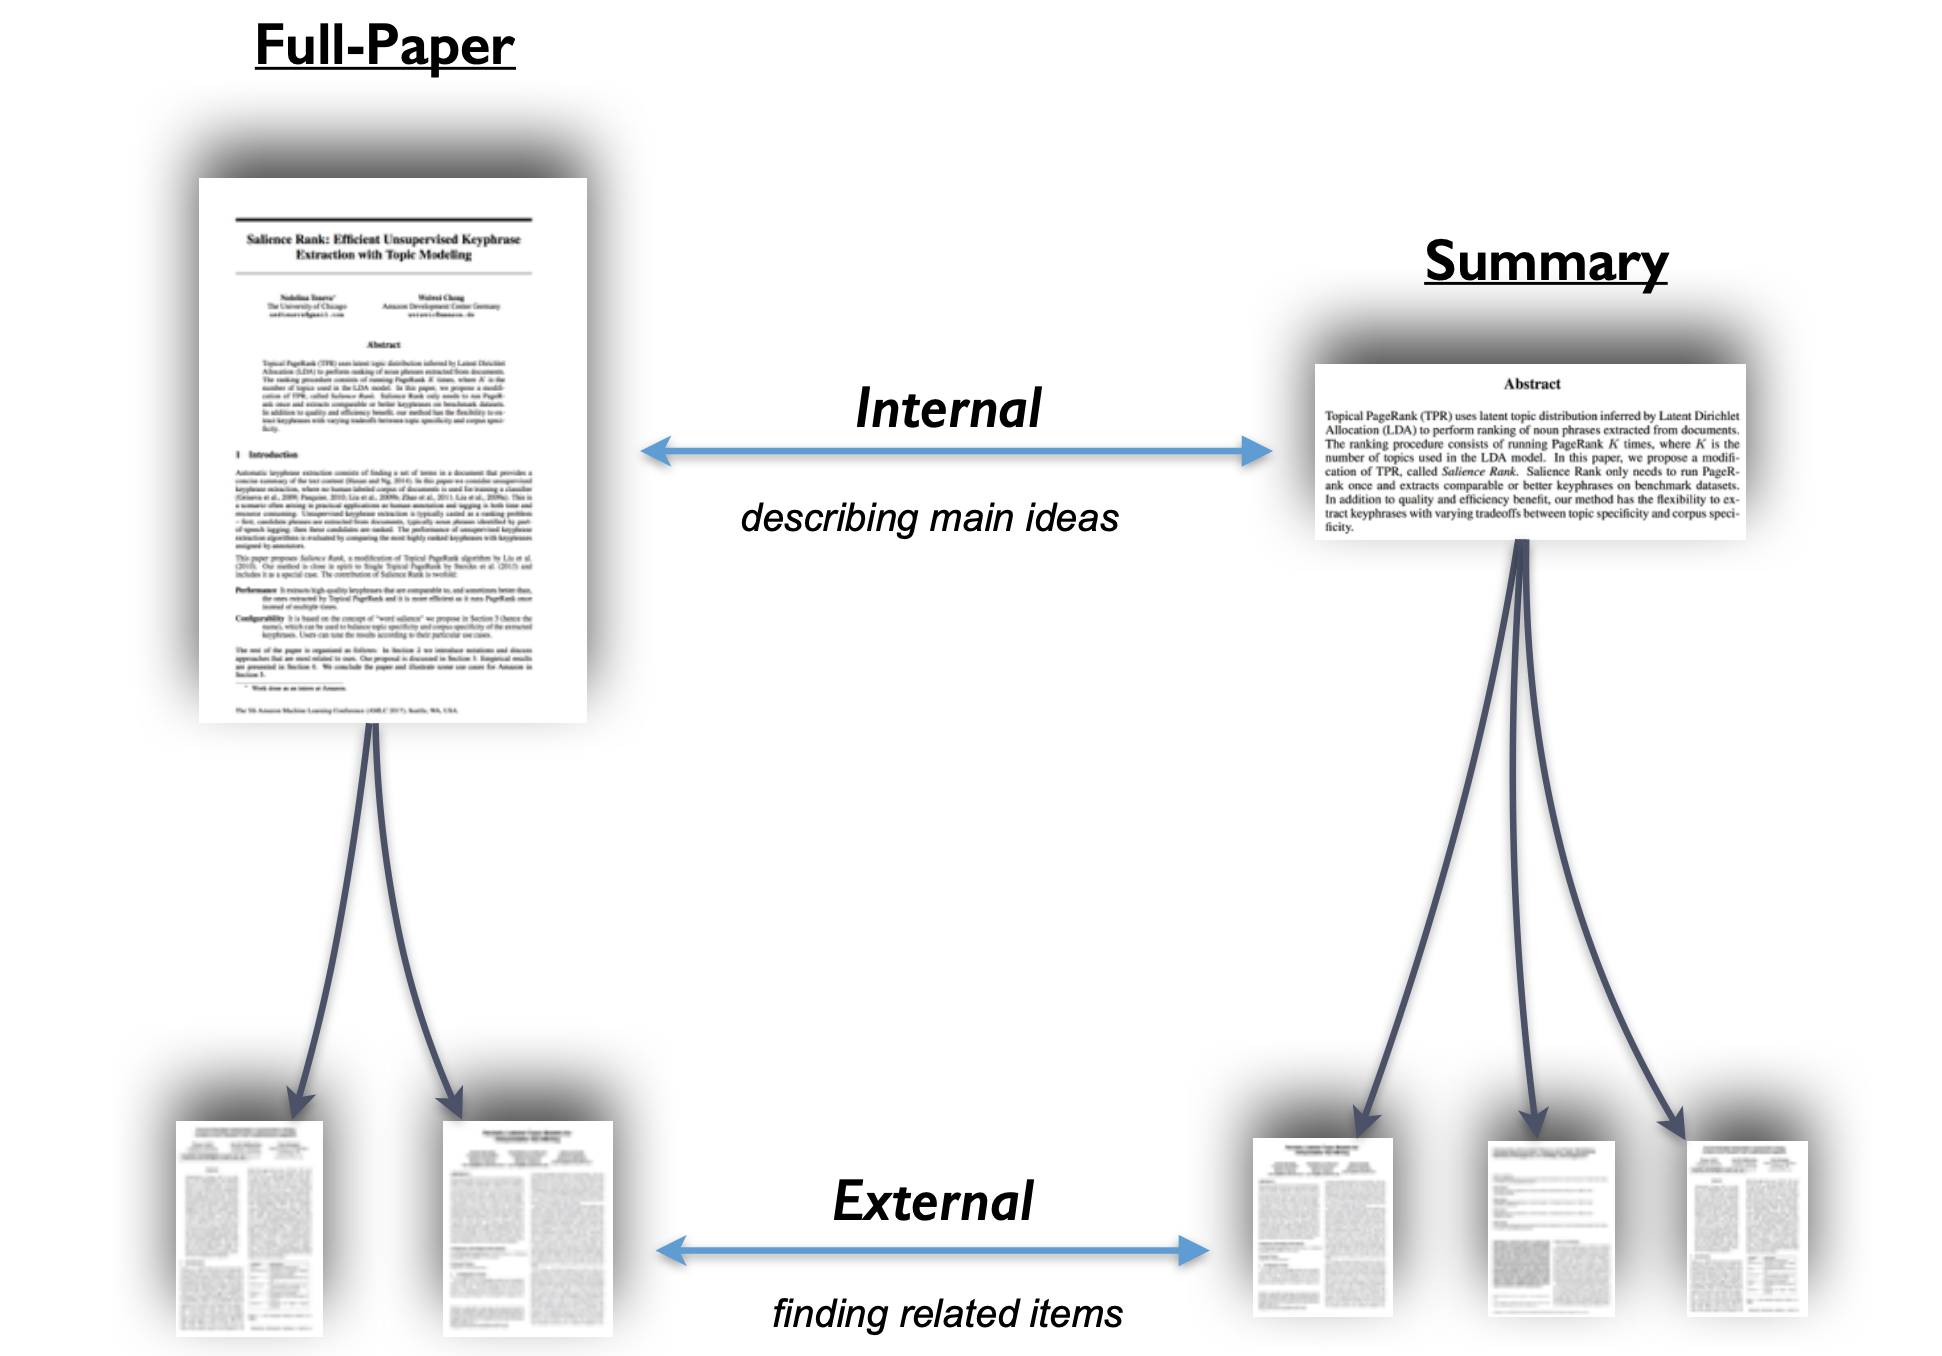
\includegraphics[scale=0.24]{internal-external.png}
\caption{Internal and External Representativeness. }
\label{fig:representativeness}
\end{figure}


An analysis about the \textit{representativeness} of research article summaries based on topic distributions is presented in this section, considering those based exclusively on abstracts and those based on their discursive structure (\textit{approach}, \textit{challenge}, \textit{background}, \textit{outcomes} and \textit{future work})\citep{SimoneTeufel2010}. The \textit{representativeness} of a summary with respect to the original full-text is assumed as the degree of relation with the original one (\textit{internal-representativeness}), along with the capacity of mimicking the full text when finding related items (\textit{external-representativeness}). In order to quantify this notion of internal-external representativeness, a probabilistic topic model is trained to have a vectorial representation of each text retrieved from a paper: full content-based and summary-based (Figure \ref{fig:representativeness}). The vectorial representations of full-papers is used to measure the distance between them and those derived from abstract or summaries (\textit{internal-representativeness}), and also to find similar documents (\textit{external- representativeness}) based on the distance between their vectorial representations. An upper distance threshold is specified to filter less similar pairs and compose a set of related papers for each paper. Then, a comparison in terms of \textit{precision} and \textit{recall} is performed between sets obtained by only using the vectorial representation of full-papers, against sets produced by using other kind of summaries.

\subsection{Research Articles Summaries}
\label{sec:annotator}
Some approaches have been proposed to summarize scientific articles \citep{Cohan2015} taking advantage of the citation context and the document discourse model. We have used the scientific discourse annotator proposed by \citep{Ronzano2015} to automatically create summaries from research papers by classifying each sentence as belonging to one of the following scientific discourse categories: \textit{approach}, \textit{challenge},  \textit{background}, \textit{outcomes} and \textit{future work}. These categories were identified from the schemata proposed by \citep{Teufel2009} with an original purpose of characterizing the content of Computer Graphics papers. 

The annotator is based on a Support Vector Machine classifier that combines both lexical and syntactic features to model each sentence in a paper. The tool\footnote{http://backingdata.org/dri/library/} was integrated in our \textit{librAIry} framework through the \textit{Rhetoric Module}\footnote{https://github.com/librairy/annotator-rhetoric} to automatically annotate research papers with their rhetorical content.

\begin{figure}[!htbp]
\centering
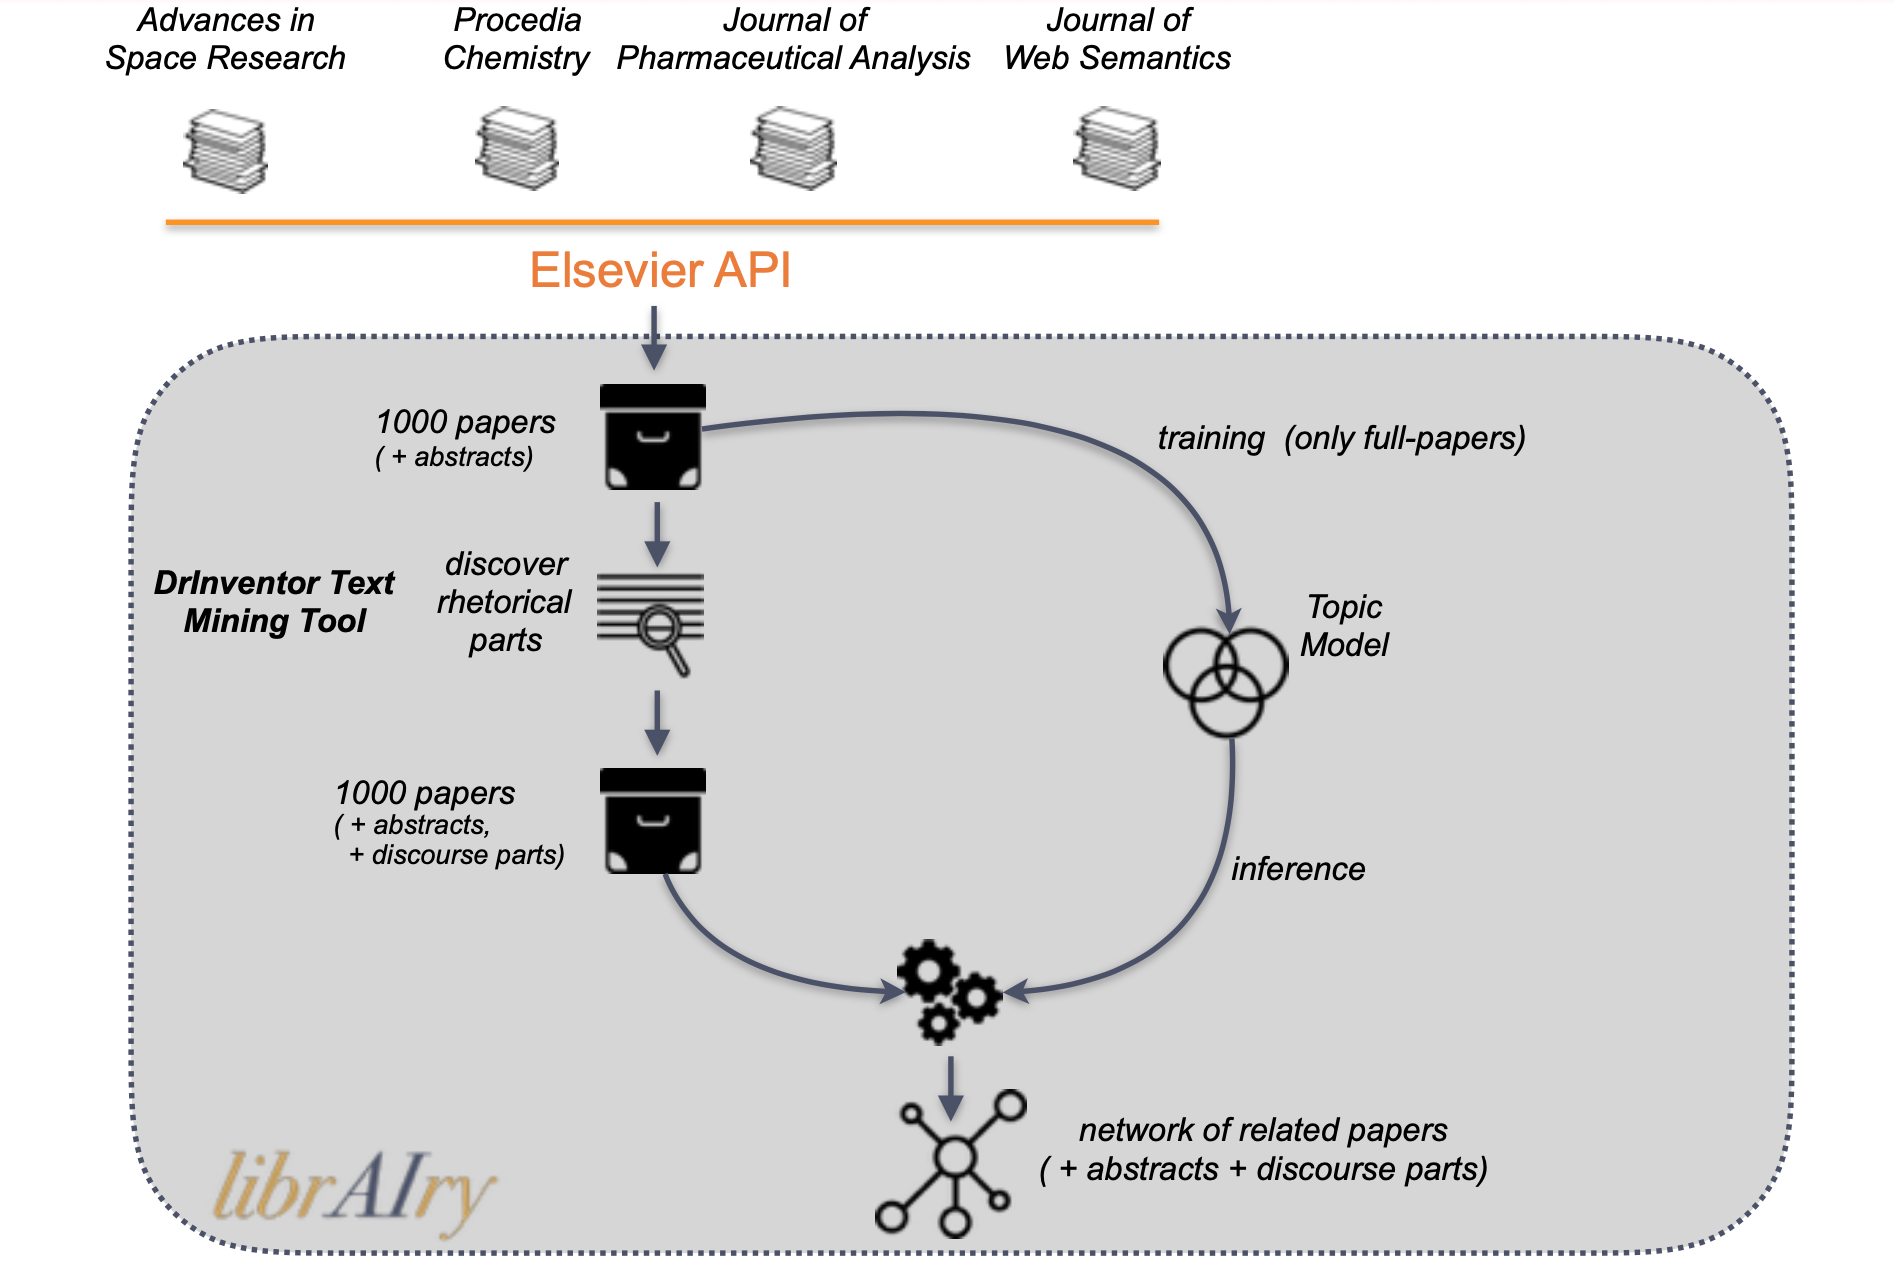
\includegraphics[scale=0.40]{similarity-experiment.png}
\caption{Experiment to analyze the ability of topic-based representations to create relations from summaries \textit{vs} full-texts. }
\label{fig:similarity-experiment}
\end{figure}

\subsection{Feature Vectors}
\label{sec:topicmodel}
A representational model is required not only to measure distances between text fragments but, more importantly, to help to understand the differences in their content. As seen in Section \ref{sec:topic-explainability}, topic models are widely used to uncover the latent semantic structure from text corpora. In particular, Probabilistic Topic Models represent documents as a mixture of topics, where topics are probability distributions over words. Latent Dirichlet Allocation (LDA)\citep{Blei2003} is the simplest \textit{generative} topic model that makes it possible to characterize documents not previously used during the training task. This is a key feature for our evaluations because, although the model used for the experiments will be trained from the full-content of papers, it will be also used to describe the texts summaries.

Thus, we have used a LDA model to describe the inherent topic distribution of papers in the corpus. Some hyper-parameters need to be estimated: the \textit{number of topics (k)}, the  concentration parameter ($\alpha$) for the prior placed on documents' distributions over topics and the concentration parameter ($\beta$) for the prior placed on topics’ distributions over terms. Since the target of this experiment is not to evaluate the quality of the representational model, but to compare their topic distributions, we accepted as valid values those widely used in the literature: $\alpha=0.1$, $\beta=0.1$ , and $k=2*\sqrt{n/2}=44$ where $n$ is the size of the corpus.



\subsection{Similarity Measure}
Feature vectors in Topic Models are topic distributions expressed as vectors of probabilities. Hence we opt for \textit{Jensen-Shannon divergence} (JS) (See Section \ref{sec:related-work})  instead of the commonly used \textit{Kullback-Liebler divergence} (KL). The reason for this is that KL is not defined when a topic distribution is zero and is not symmetric, what does not fit well with semantic similarity measures which in general are symmetric \citep{Rus2013}. JS considers the average of the distributions as follows :

\begin{equation}
JS(p,q) = \sum\limits_{i=1}^T p_{i}*\log \frac{2*p_{i}}{p_{i}+q_{i}}  +  \sum\limits_{i=1}^T q_{i}*\log \frac{2*q_{i}}{q_{i}+p_{i}}
\label{eq:jsd}
\end{equation}
where  $T$ is the number of topics and $p,q$ are the topics distributions.

And the \textit{similarity measure} used in our analysis is based on the JS transformed into a similarity measure as follows \citep{Dagan1998} :

\begin{equation}
similarity(D_i , D_j) = 10^{- JS(p,q)}
\label{eq:simcontent}
\end{equation}
where  $D_i,D_j$ are the documents and $p,q$ the topics distributions of each of them.

\subsection{Evaluation}
\label{sec:topic-relevance-experiments}

The corpus used in the experiments was created by combining journals in different scientific domains such as \textit{Advances in Space Research}, \textit{Procedia Chemistry}, \textit{Journal of Pharmaceutical Analysis} and \textit{Journal of Web Semantics} (Figure \ref{fig:similarity-experiment}). In total 1,000 papers were added, 250 from each journal. Both the abstract and the \textit{full-content} of these documents were directly retrieved from the Elsevier API \footnote{https://dev.elsevier.com} by using our \textit{Harvester module} \footnote{https://github.com/librairy/harvester-elsevier}. The code used to perform the analysis along with the results obtained are publicly available\footnote{https://github.com/librairy/study-semantic-similarity}.

Since the annotation process to automatically discover the rhetorical parts of a research paper (Section ~\ref{sec:annotator}) is sensitive to the structure of the phrases that are used when writing the text, only $20\%$ of papers in the corpus could be fully annotated with all the fragments considered. In fact, these categories are not present in the same proportion in the corpus: \textit{approach} ($90\%$), \textit{background} ($78\%$), \textit{outcome} ($73\%$), \textit{challenge} ($57\%$) and \textit{future work} ($21\%$)

\subsubsection{Internal Representativeness}

The \textit{internal-representativeness} of a text measures the similarity of a summary against the original full-text. This measure is based on the JS between the topic distribution of each of them. 

\begin{figure}[!htbp]
  \center
  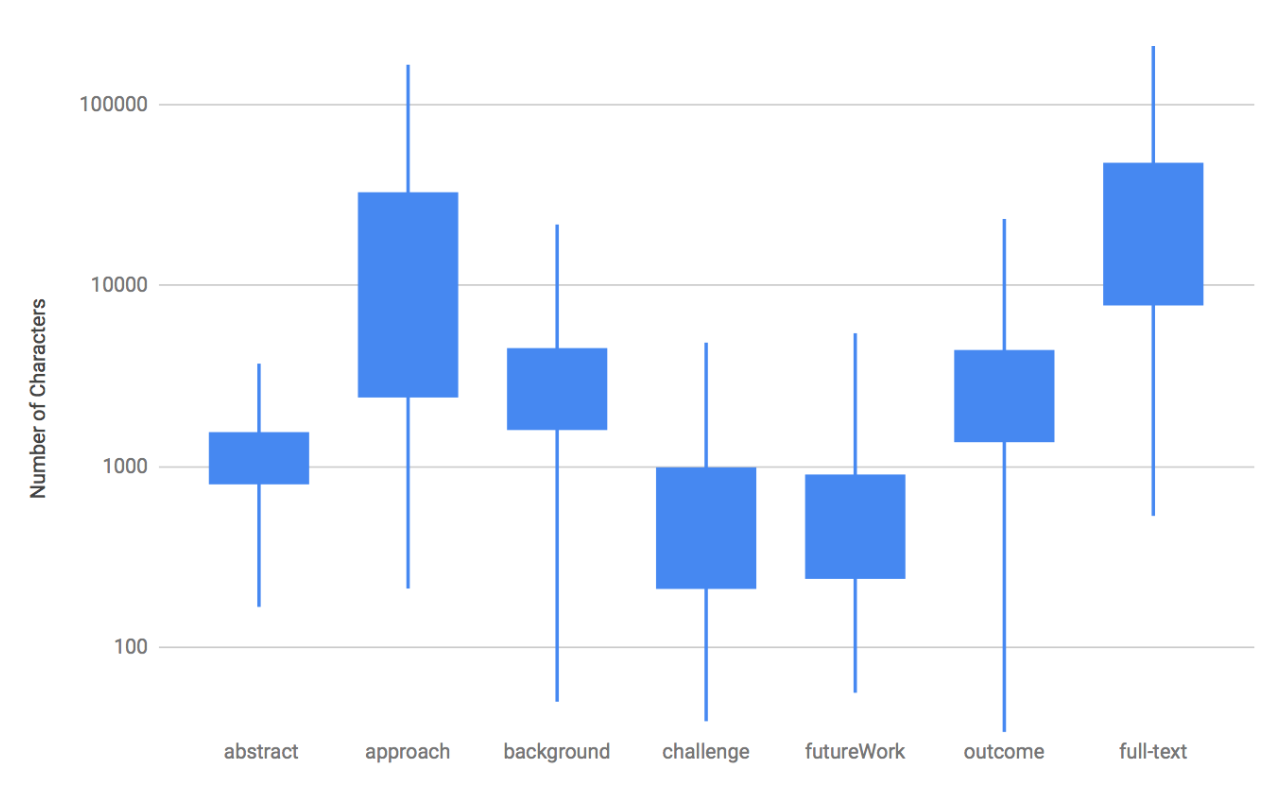
\includegraphics[scale=0.4]{size.png}
  \caption{length of summaries.}
  \label{fig:size}
\end{figure}

\begin{figure}[!htbp]
  \center
  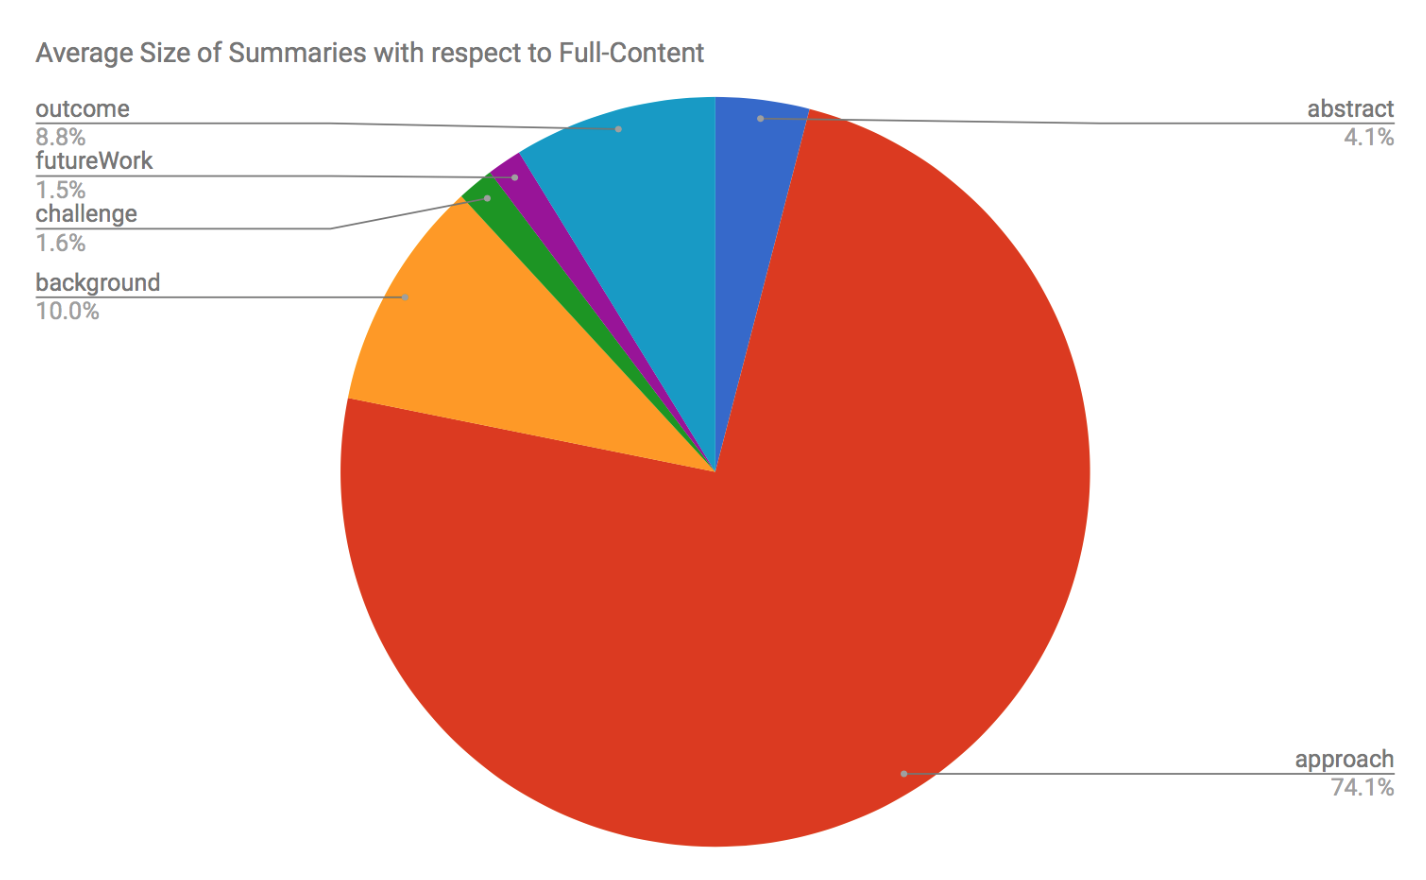
\includegraphics[scale=0.4]{relativeSize.png}
  \caption{length of text parts.}
  \label{fig:relativeSize}
\end{figure}

Since LDA considers documents as \textit{bag-of-words}, the text length (e.g. full-content or summaries) affects the accuracy of the topic distributions inferred by the topic model described in Section~\ref{sec:topicmodel}. The occurrences of words in short texts are less discriminative than in long texts where the model has more word counts to know how words are related \citep{Hong2010}. In view of the above, the \textit{approach}, the \textit{background} and the \textit{outcome} content of a paper generate more accurate topic distributions than those created from other approaches such as the abstract (Figure \ref{fig:size}). Also, the relative presence of each of them in a paper (figure~\ref{fig:relativeSize}) shows an unexpected result when compared to the IMRaD format \citep{Nair2014}. This style proposes to distribute the content of an abstract, and by extension the full-paper, as follows: \textit{Introduction}(25\%), \textit{Methods}(25\%), \textit{Results}(35\%) and \textit{Discussion}(15\%). However, the results (figure~\ref{fig:relativeSize}) show that \textit{Method} section (\textit{approach} content) is more extensive than \textit{Results} section (\textit{outcome} content) in our corpus.

All pairwise similarities between full-papers, abstracts and rhetorical-based summaries are calculated to measure the \textbf{\textit{internal-representativeness}} of a summary with respect to the original text, i.e. the topic-based similarity value (equation~\ref{eq:simcontent}) between the probability distributions of the full-text and each of the summaries. Results (table~\ref{tab:irepresentativeness}) suggest that summaries created from the \textit{approach} content are more representative than others, i.e. the distribution of topics describing the text created from the \textit{approach} content is the most similar to the one corresponding to the full-content of the paper.

\begin{table}[!htb]
    \centering
        \begin{tabular}{l*{6}{c}r}\hline
                        & Min & Lower Quartile & Upper Quartile & Max & Dev  & Median \\
          \hline
          abstract & 0.0489 & 0.9109 & 0.9840 & 1.0000 & 0.1443 & 0.9741 \\
          \textbf{approach} & \textbf{0.0499} & \textbf{0.9969} & \textbf{1.0000} & \textbf{1.0000} & \textbf{0.0872} & \textbf{0.9998} \\
          background & 0.0463 & 0.8967 & 0.9937 & 0.9988 & 0.2037 & 0.9822 \\
          challenge & 0.0426 & 0.7503 & 0.9517 & 0.9940 & 0.2224 & 0.8829 \\
          futureWork & 0.0000 & 0.6003 & 0.9435 & 0.9948 & 0.2842 & 0.8814 \\
          outcome & 0.0485 & 0.9267 & 0.9925 & 0.9990 & 0.1721 & 0.9835 \\
        \end{tabular}
    \caption{ Accuracy results when comparing the most related articles using a summary (e.g. abstract, approach, background, challenge, future work or outcome), with those obtained using the full-text of the article (\textit{internal-representativeness}).}\label{tab:irepresentativeness}
\end{table}

\subsubsection{External-Representativeness}  

The \textit{external-representativeness} metric tries to measure how different is the set of related documents obtained from summaries with respect to those derived from the original full-text. In terms of \textit{precision}, \textit{recall} and \textit{f-measure}, a comparison has been performed to analyze the behavior of the summaries when trying to discover related content compared to use the full-text of the article.

\begin{figure}[!htbp]
  \center
  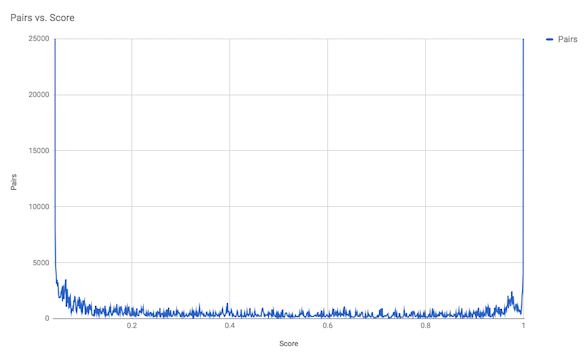
\includegraphics[scale=0.45]{similarities.png}
  \caption{number of pairwises by similarity score (rounded up to two decimals).}
  \label{fig:similarities}
\end{figure}


By using the same topic model previously created, similarities among all pairs of documents were also calculated according to equation~\ref{eq:simcontent}. Then, a minimum score or similarity threshold is required to define when a pair of papers are related. Each threshold is used to create a gold-standard which relates articles to others based on their similarity values. In order to discover that lower bound of similarity, a study about trends in the similarity scores (fig~\ref{fig:similarities}) as well as distributions of topics in the corpus (fig~\ref{fig:articleTopics}) was performed. We can see that topics are not equally balanced across papers. This fact generates separated groups of strongly related papers. We think this phenomena is due to our usage of a corpus created from journals where different domains are equally balanced. Then, we considered a similarity score equals to $0.99$ (fig ~\ref{fig:similarities}) as the threshold from which strong relations appear. However, to cover different interpretations of similarity, from those based on sharing general ideas or themes to those that imply to share a more specific content, the following list of thresholds was considered in the experiments: 0.5, 0.6, 0.7, 0.8, 0.9, 0.95 and 0.99.


For each similarity threshold, a gold-standard was created based on considering as related those papers with a similarity value upper than the selected threshold. Results ( figure ~\ref{fig:precision}) comparing the related papers inferred from the full-content with those inferred from the partial-content representation (i.e. abstract or rhetorical parts) suggest that strongly related papers are mainly discovered by using the summary created from the \textit{approach} section. The reason for this may be based on the average size of this type of summaries or the particular content included in this part of a paper. While other summaries include more general-domain words, the \textit{approach} content includes more specific words that describe the method or the final objective of the paper. So, for higher similarity thresholds, i.e. for strongly related papers, the recommendations discovered by using the \textit{approach} are more precise than those discovered by using the abstract.

\begin{figure}[!htbp]
  \center
  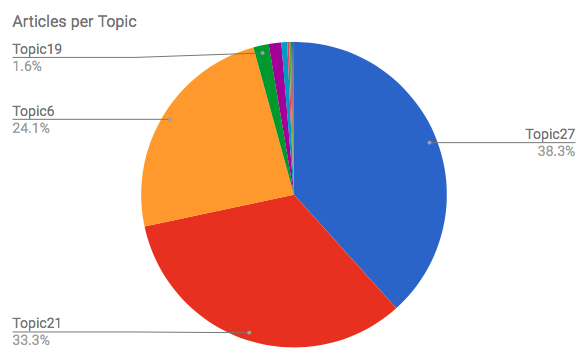
\includegraphics[scale=0.4]{articlesTopic.png}
  \caption{topics per article with value above 0.5.}
  \label{fig:articleTopics}
\end{figure}


In terms of \textit{recall} (figure ~\ref{fig:recall}), the upward trend followed by the \textit{approach}, the \textit{outcome} and the \textit{background} content remarks the assumption of summaries containing key words allow to discover more similar papers than others. Moreover, since \textit{recall} overlooks false-negatives classifications, it suggests that these parts of a research paper share more words than others with strongly related papers but they may also present commonalities with highly related papers, except in case of \textit{approach} which still exhibits higher \textit{precision}.

\begin{figure}[!htbp]
  \center
  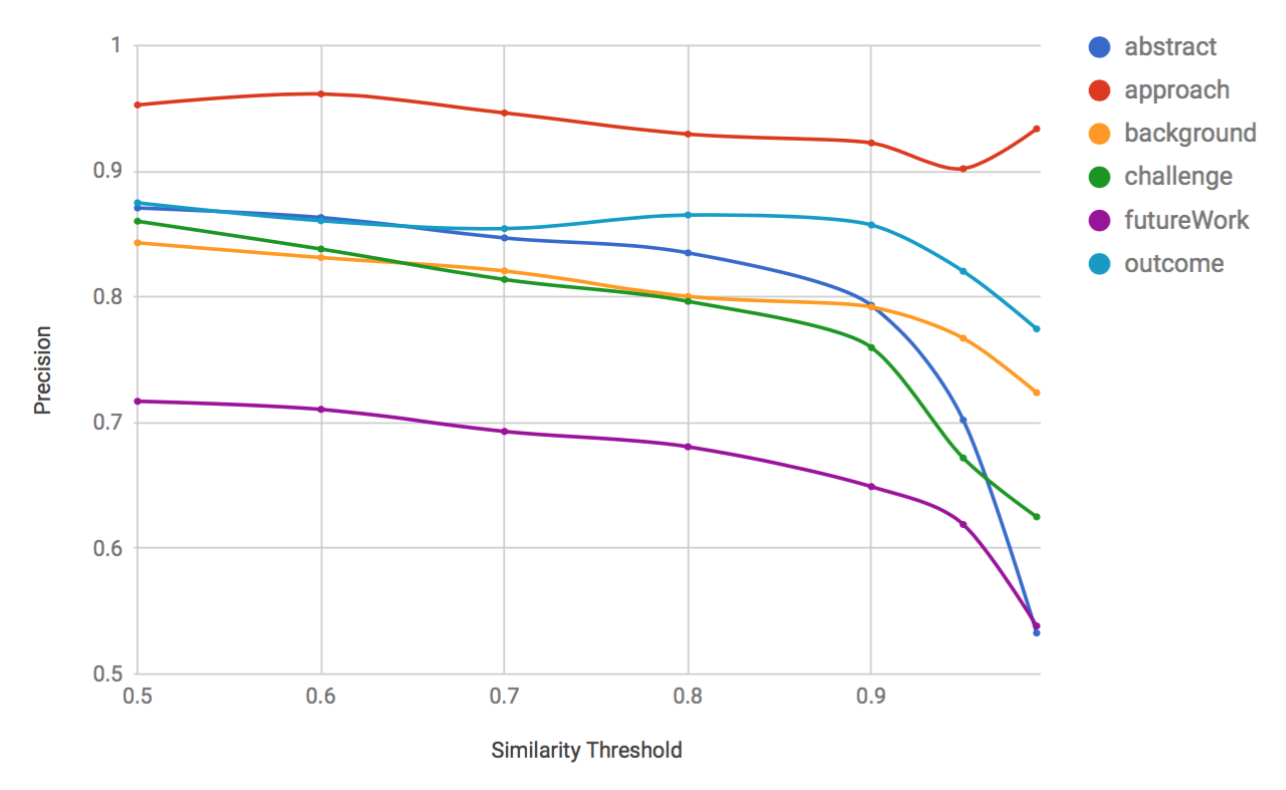
\includegraphics[scale=0.4]{precision.png}
  \caption{Precision at different similarity thresholds.}
  \label{fig:precision}
\end{figure}

\begin{figure}[!htbp]
  \center
  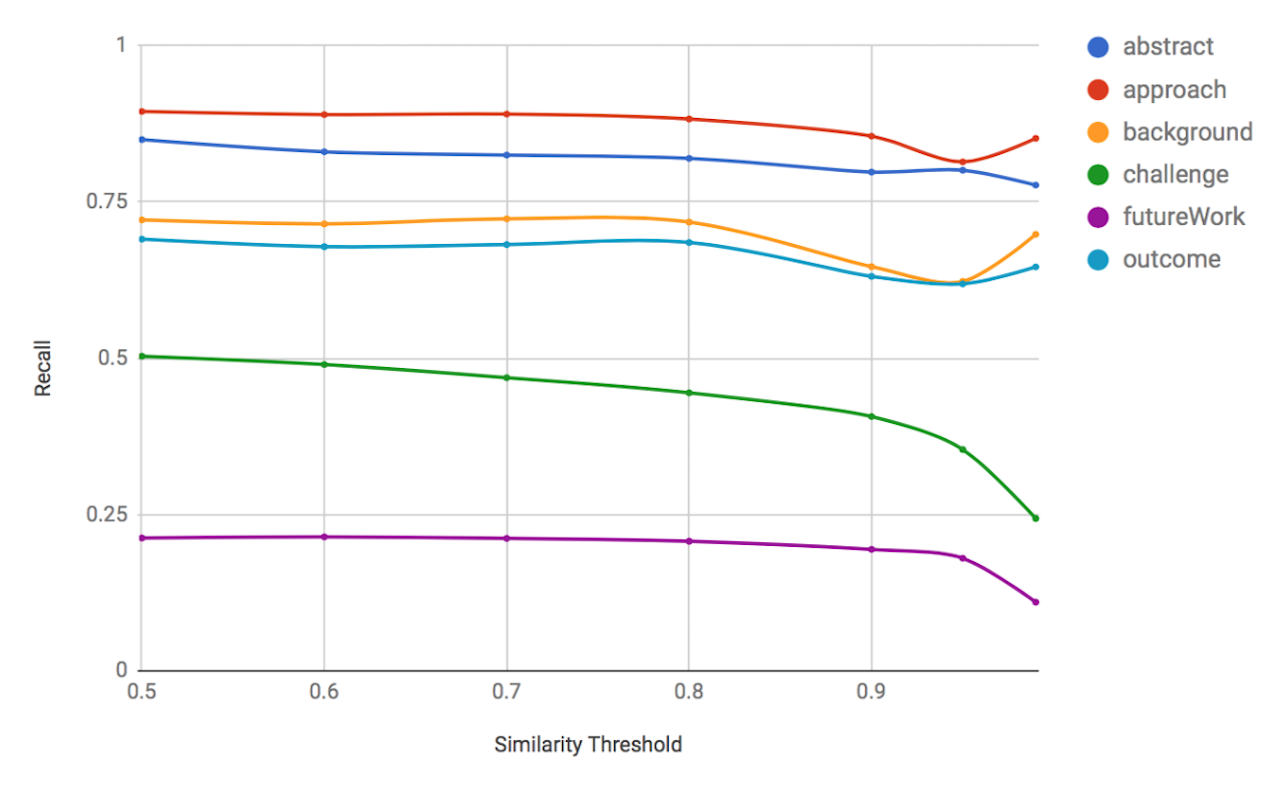
\includegraphics[scale=0.4]{recall.png}
  \caption{Recall at different similarity thresholds.}
  \label{fig:recall}
\end{figure}


As expected, only summaries created from the \textit{approach}, the \textit{outcome} and the \textit{background} content maintain high accuracy values (fig~\ref{fig:fmeasure}) even for high similarity thresholds. Along with the results showed in figure~\ref{fig:stdeviation}, where the same three rhetorical classes present the lowest standard deviation over the \textit{f-measure}, they can be considered as the most robust summaries containing the ideas that better characterize the paper compared to others.


\subsection{Conclusion}
Topic-based relations have been studied among scientific documents based on their abstract sections with respect to summaries corresponding to their scientific discourse categories. For this purpose, two novel measures have been proposed: (1) \textit{internal-representativeness} and (2) \textit{external-representativeness}.

Results show that summaries created from the \textit{approach}, \textit{outcome} or \textit{background} content of a paper describe more accurately its full-content in terms of overall ideas and related documents than abstracts. Although those summaries are more extensive in number of characters than other with similar \textit{precision} such as the abstract content, they have proven to be particularly helpful  discovering strongly related papers, i.e. papers with a similarity value close to 1.0.

\begin{figure}[!htbp]
  \center
  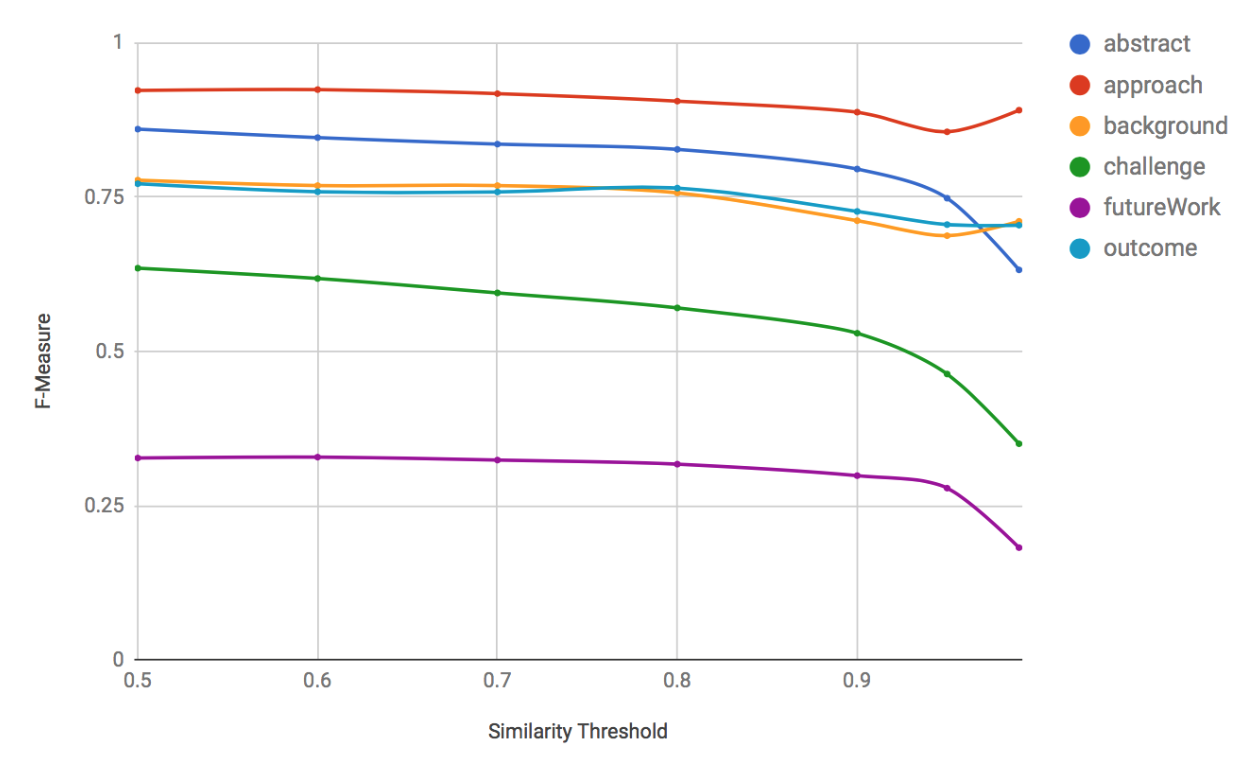
\includegraphics[scale=0.4]{fmeasure.png}
  \caption{f-measure performance.}
  \label{fig:fmeasure}
\end{figure}

\begin{figure}[!htbp]
  \center
  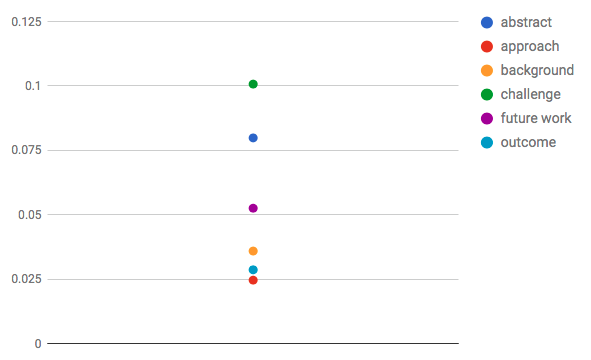
\includegraphics[scale=0.4]{stdeviation.png}
  \caption{f-measure deviation.}
  \label{fig:stdeviation}
\end{figure}


\section{Topic-based Clustering}
\label{sec:topic-clustering}

Once we have a better understanding of the behavior of topic models to represent texts, and the relationships that can be derived from them, we examine their usefulness in browsing document collections. A way to explore the knowledge inside document collections is by moving from one information element to another based on certain criteria that relates them. This approach requires to calculate a similarity matrix with all possible comparisons between elements, so we can later select the most pertinent ones. Since computing a $n \times n$ matrix takes $O(n^2)$ time, obtaining all possible pairs of similarities in a large collection of documents can be unfeasible because of the quadratic cost of comparing every pair of elements.

In order to reduce the complexity, some approaches have introduced mechanisms (mainly pre-election methods) to alleviate the problem of making this calculation over the whole set of pairs in the collection. However those methods are still quite costly.

In this section we propose a novel clustering technique based on topic model distributions that reduces the complexity to find relations between documents in a large corpus of textual documents, without compromising efficiency and providing additional information about relations. A detailed description of our algorithm is given in Section ~\ref{sec:clustering-approach}. The experiments to verify the efficiency and effectiveness of our clustering algorithms using real data, and demonstrate that our approach is competitive enough against both a centroid-based and a density-based clustering baselines are described in Section ~\ref{sec:clustering-experiments}. The most relevant results and conclusions are finally presented in Section ~\ref{sec:clustering-conclusion}.

\begin{figure}
  \centering
  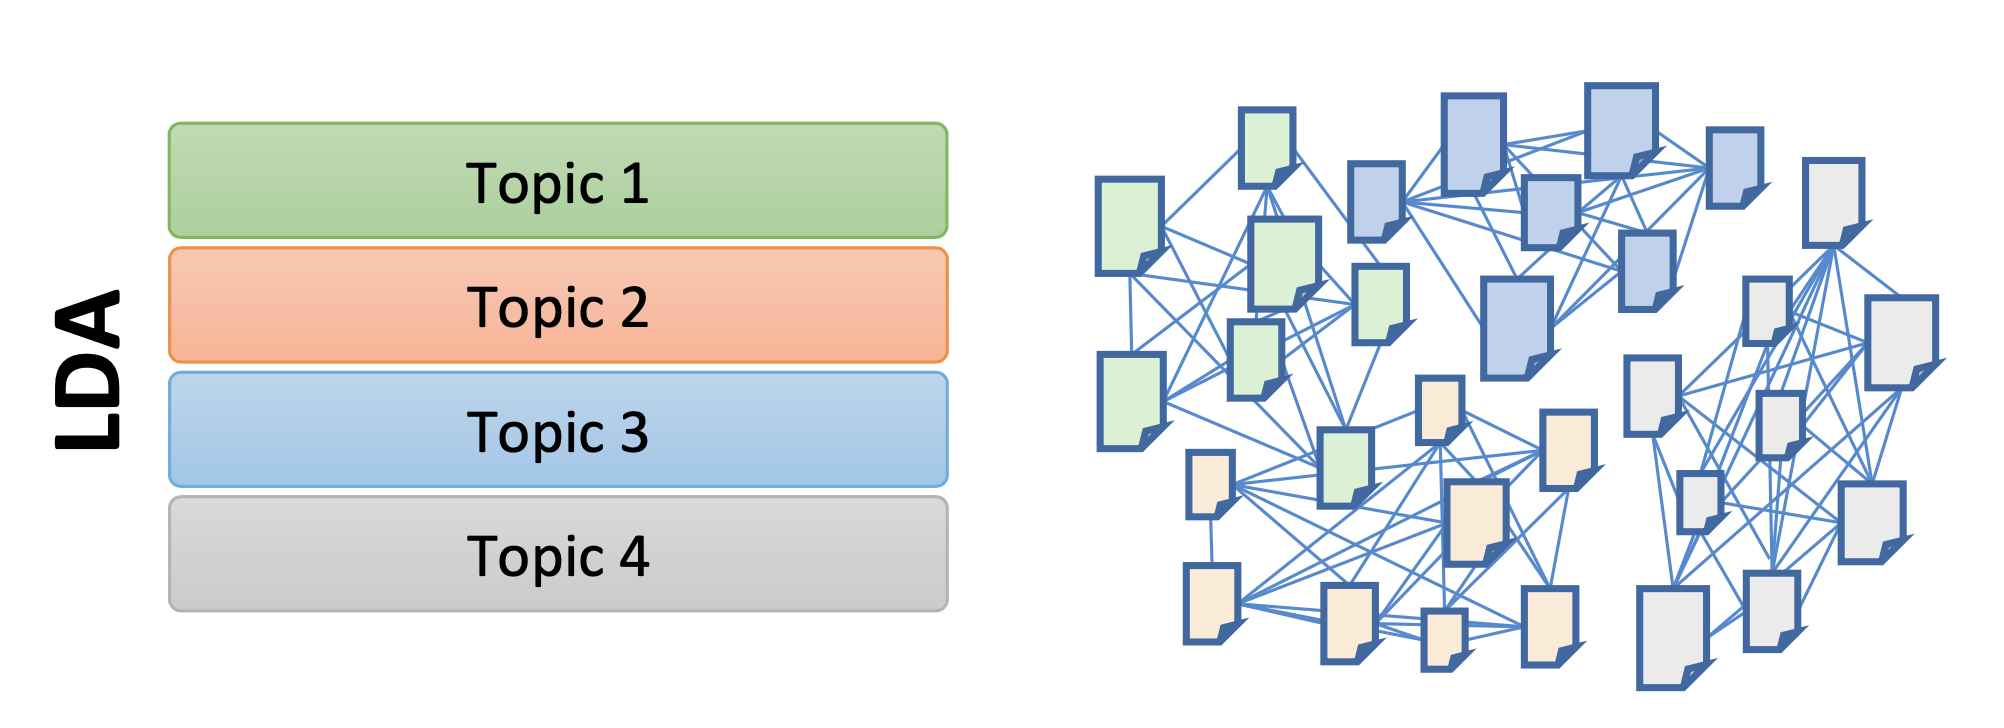
\includegraphics[scale=0.37]{lda-cluster.png}
  \caption{Probabilistic Topic Models, and in particular Latent Dirichlet Allocation (LDA), can efficiently divide the search space and speed up the process of finding relations among documents inside big collections.}
  \label{fig:lda-cluster}
\end{figure}



\subsection{Most Relevant Topics}
\label{sec:clustering-approach}

Our algorithm to identify the most relevant topics draw inspiration from other clustering techniques to divide the initial space of elements into smaller sub-groups where the complexity of calculating all possible distances is significantly reduced. Existing unsupervised approaches based on centroids or density measures require to make comparisons between elements to find groups of similar elements in the collection. They usually follow an iterative methodology to produce the final solution, based on calculating distances between the elements inside each intermediate state. A na{\"i}ve approach would need to calculate all possible distances between elements, which takes $O(n^2)$ time for a $n \times n$ matrix. That makes it impossible to apply such techniques on large collections of documents, since the cost of comparing each element with the others escalates quickly. For those big volumes of data, a clustering task that only takes linear time to discover the clusters can significantly alleviate this problem. For example, a classification method that does not require any other data except the element information to assign the item to the corresponding cluster will take $O(n)$ time to compose those groups.

The classification method needs to take advantage of both the vectorial representations of the documents and the similarity measure used to relate them in a corpus. Since the representational model considered is based on Probabilistic Topic Models (and more specifically on LDA), the classification method leverages on the particular behavior of Dirichlet distributions, which describes each document by a density vector where the sum of all the probability values must be equal to 1.0. Thus, analyzing the relations between the topics that compose a topic distribution becomes more important than comparing their probability values with another topic distribution.

Our hypothesis is that, \textit{given a collection of topic distributions, an unsupervised classification with high precision and linear computing time can be performed by considering only the topic distribution of each document and without needing to further compare it with other document's distributions}.
% \citep{Towne2016}

All algorithms have been compared in terms of \textit{cost}, \textit{effectiveness} and \textit{efficiency} \citep{Halkidi2001a}. \textit{Cost} is based on the number of pairwise similarity checks. \textit{Effectiveness} handles relevance measures such as \textit{precision} and \textit{recall}. And \textit{efficiency} tries to measure the overall balance between \textit{cost} and \textit{effectiveness}. More details about those measures will be included in Section~\ref{sec:clustering-experiments}.

\subsubsection{Trends-based Clustering Method}

Topic distributions are formalized as probability distributions following a Dirichlet distribution, so their probability values sum to 1. In this way, the relevance of a topic is influenced and at the same time influences the relevance of the others items in the distribution. Our first approach named \textit{Trends on Dirichlet distribution-based Clustering} (TDC) considers changes in the relevance, i.e. probability values of the topics instead of directly relying on the scores associated to a given topic distribution (Figure \ref{fig:tdc-cluster}). It expresses the oscillations between topic weights considering a fixed order between them. The order can be any, as long as it remains constant in all distributions. Thus, a \textit{probability-vector} composed by $n$ density values is translated to a \textit{trend-expression} made out of $n-1$ trend-values such as (1) upward, (2) downward and (0) sustained. This \textit{trend-expression} will identify the cluster  the distribution falls into, and therefore the corresponding item belongs to. TDC is defined as:
\begin{equation}
TDC(P)=T
\end{equation}
\begin{conditions}
 T_{i}     & 1,  when $P_i < P_{i+1}$ \\
 T_{i}     & 2,  when $P_i > P_{i+1}$ \\   
 T_{i} 	   & 0,  when $P_i = P_{i+1}$
\end{conditions}
For example, given the distribution $P_1=[0.23, 0.18, 0.33, 0.13, 0.13]$, the assigned cluster will be $T=2120$. The first value is $2$ because $0.23$ is greater than $0.18$ (same for other values).

\begin{figure}[!htbp]
  \centering
  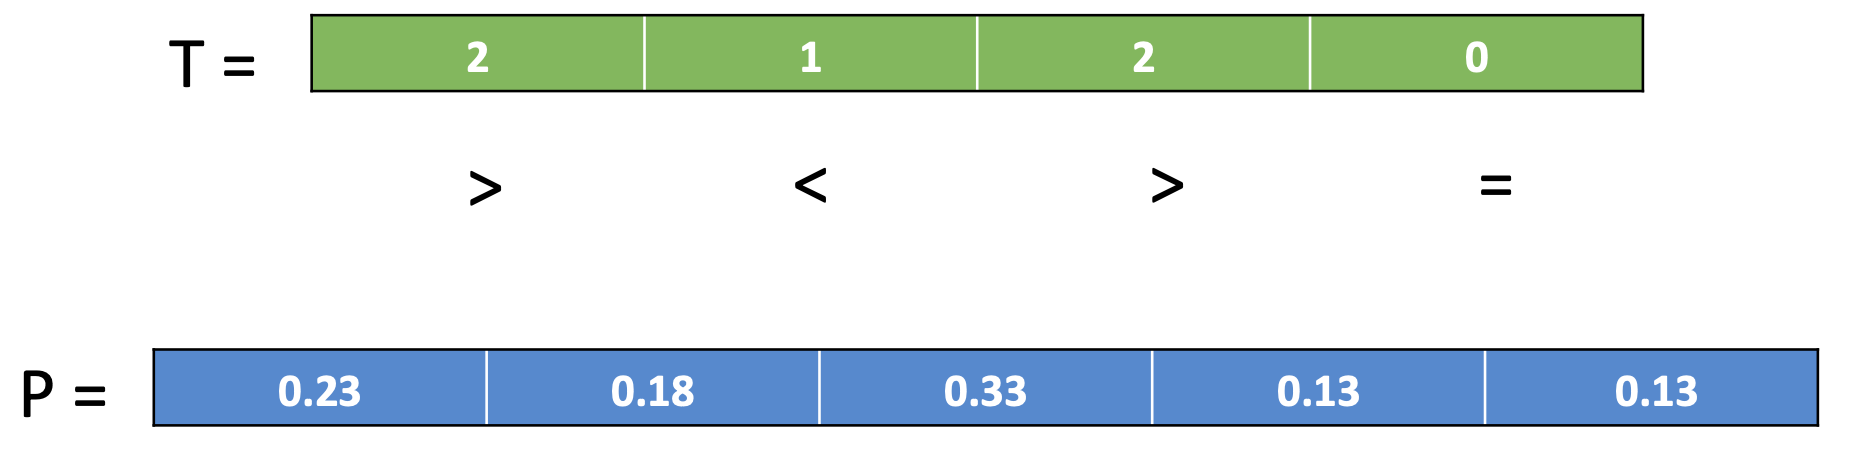
\includegraphics[scale=0.33]{tdc-cluster.png}
  \caption{TDC considers variations across consecutive topics inside a document’s topic distribution.}
  \label{fig:tdc-cluster}
\end{figure}


\subsubsection{Ranking-based Clustering Method}

We propose a clustering technique named \textit{Ranking on Dirichlet distribution-based Clustering} (RDC) that only considers the top $n$ topics from the ranked list of probability distributions to classify similar topic distributions (Figure \ref{fig:rdc-cluster}). It is based on the focal document selection proposed by \citep{Towne2016} to validate LDA-based similarity algorithms against human perception of similarity. RDC is defined as:
\begin{equation}
RDC(P)=R
\end{equation}
where  $\forall i \in R, R_i>=R_{i+1}$ and $\forall j \in P, R_1>=P_j$

This is based on the assumption that the highest weighted topics have a high influence in the rest of topics in terms of calculating distances, when comparing continuous multivariate probability distributions. Since similarity measures (Section ~\ref{sec:related-work}) based on probability distributions are oriented to determine the uncertainty of the distribution, when a mixture of probability distributions is considered, as in the case of Topic Models, the top $n$ distributions (i.e. the most relevant topics) should be sufficient to allow us grouping similar distributions. Taking into account the above considerations, the RDC algorithm classifies a topic distribution according to only $n$ highest probability values. For instance, given the following topic distribution: $P_2=[0.23, 0.18, 0.33, 0.13, 0.13]$, the assigned cluster is \textit{3} from RDC-1 because that is the topic with the highest weight.

\begin{figure}[!htbp]
  \centering
  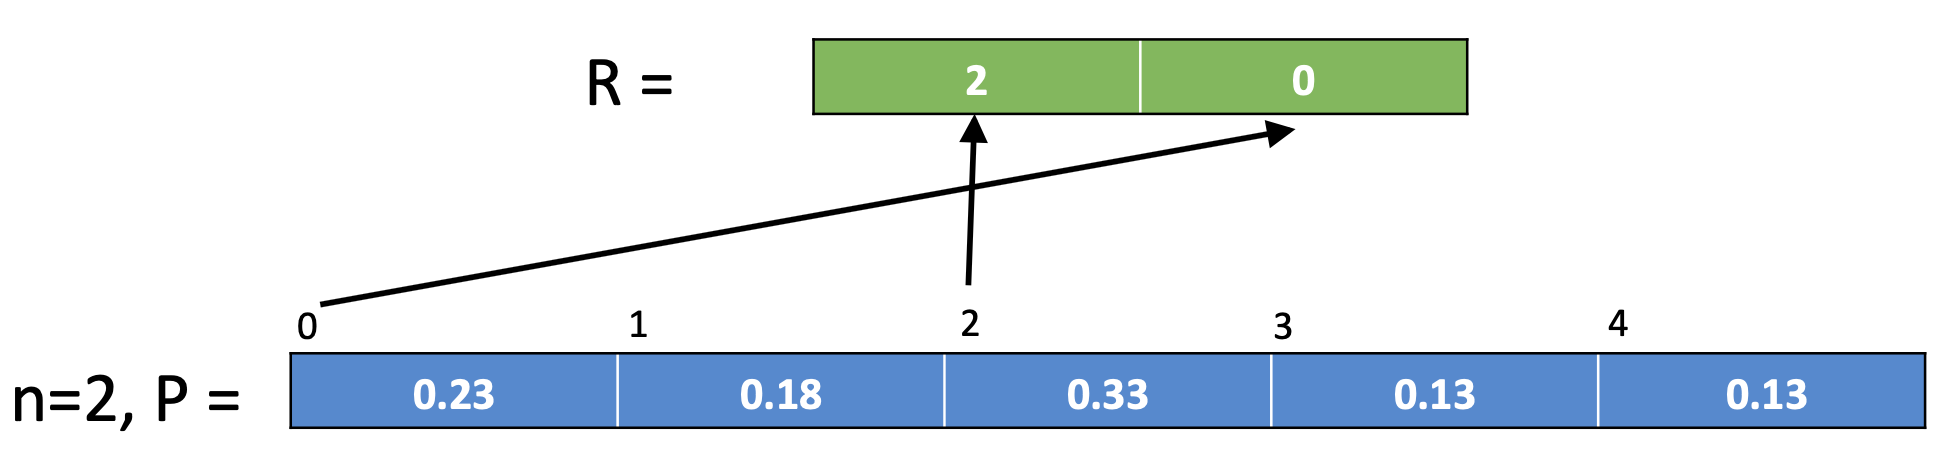
\includegraphics[scale=0.33]{rdc-cluster.png}
  \caption{RDC only considers the top n topics from the ranked list of probability distributions.}
  \label{fig:rdc-cluster}
\end{figure}


\subsubsection{Cumulative Ranking-based Clustering Method}

A variant of the previous algorithm, named \textit{Cumulative Ranking on Dirichlet distribution-based Clustering} (CRDC), also aims to discover the most representative topics that can help to group similar topic distributions. While RDC is based on a fixed number of topics, CRDC is based on the cumulative sum of the weights of the highest topics (Figure \ref{fig:crdc-cluster}). The number of topics is now dynamically determined by a threshold, and once this threshold is reached no more topics are considered. CRDC is defined as:
\begin{equation}
CRDC(P)=C
\end{equation}
where  $\forall i \in C, C_i >=C_{i+1}$ and $\sum\limits_{i=1}^T C_i >= w$ with $T$ size of $C$, and $w$ a cumulative weight threshold.


For instance, considering a CRDC algorithm with a cumulative weight threshold of 0.9, and the following topic distribution: $P_3=[0.36, 0.58, 0.05, 0.01]$. The assigned cluster will be \textit{21}. To come up with this cluster, a ranked list of topics based on their weights is first calculated, $R_p=2|1|3|4$. Then, a sum of weights according to the order described by $R_p$ is performed. When the accumulated sum is greater than the threshold, the topics taking part of the sum will be selected to ``label'' the cluster. In this case, the cumulative weight threshold is 0.9 therefore using only the first two topics we exceed the threshold: $w=0.58+0.36=0.94$

\begin{figure}[!htbp]
  \centering
  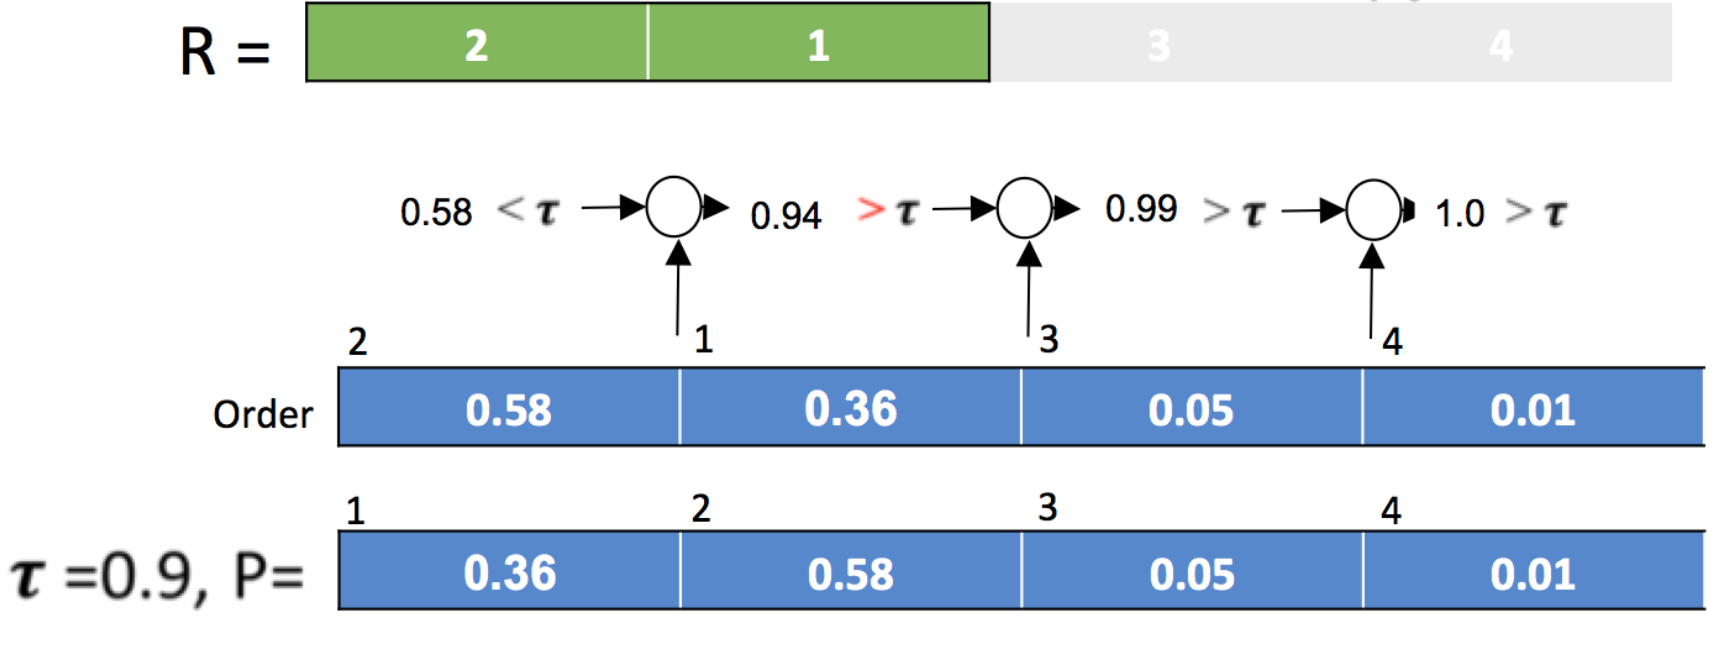
\includegraphics[scale=0.33]{crdc-cluster.png}
  \caption{CRDC only considers the top n topics until the sum of the weights of the highest topics exceeded a given threshold.}
  \label{fig:crdc-cluster}
\end{figure}


\subsection{Evaluation}
\label{sec:clustering-experiments}
In this section we present the experimental setup for evaluating our trends-based (TDC), ranking-based (RDC) and cumulative ranking-based (CRDC) clustering approaches, considering both JS divergence and He distance as similarity measures. We describe the datasets and baseline algorithms that will be used for comparison.

\subsubsection{Datasets}
\label{sec:clustering-datasets}
We used two datasets to evaluate the performance of the algorithms. The first dataset, DIRICHLET-RANDOM-MIXTURE (DRM), is synthetic\footnote{https://doi.org/10.5281/zenodo.931305}. To generate the dataset, we sampled \textit{k} probabilistic distributions from a \textit{randomly k-dimensional selector} based on Dirichlet distributions. This implies that all probabilities must to sum to 1 for each sampled point. The number of sampled points from this mixture of Dirichlet distributions is $n=1000$.

The second dataset has been created from a collection of research papers published in the \textit{Advances in Engineering Software} (AIES) journal. They were retrieved from the Springer API by using the librAIry \citep{Badenes-Olmedo2017} framework and a Topic Model based on LDA was created from them. The sample is also composed by $n=1000$ documents.

Topic models were trained from these datasets by using the criteria described by \citep{Steyvers2006}: $\alpha= 50/k$ , $\beta= 0.01$ and $k=2*(\sqrt{(n/2)})$, where $k$ is the number of topics and $n$ is the number of documents. Since both datasets contain $1000$ documents ($n$), the hyper-parameters $\alpha$ and $\beta$ are assigned as follow: $\alpha=1.136$, and $\beta=0.01$, and the number of topics is fixed to $k=44$. Further tuning of the settings is not crucial in this evaluation process, because we are not focusing on the quality of the model but on the efficiency when calculating similarities from their representational distributions.

\subsubsection{Settings}
\label{sec:clustering-threshold}
Since there is no unified criteria to select a threshold inside the distance scores spectrum that allows us to determine when two documents are similar, we decided to study the distribution of similarity values calculated from all pairwise comparisons. In Figure ~\ref{fig:similarityThreshold}, the result of grouping all similarities by the two most representative decimals, i.e. the first two decimals of the similarity value, is shown. Then, a polynomial function (red line) is approximated to describe the trend of these values. In this function, the similarity score $0.83$ emerges as a global minimum and has been used for filtering out the non-similar document pairs.

\begin{figure}[!htbp]
  \centering
  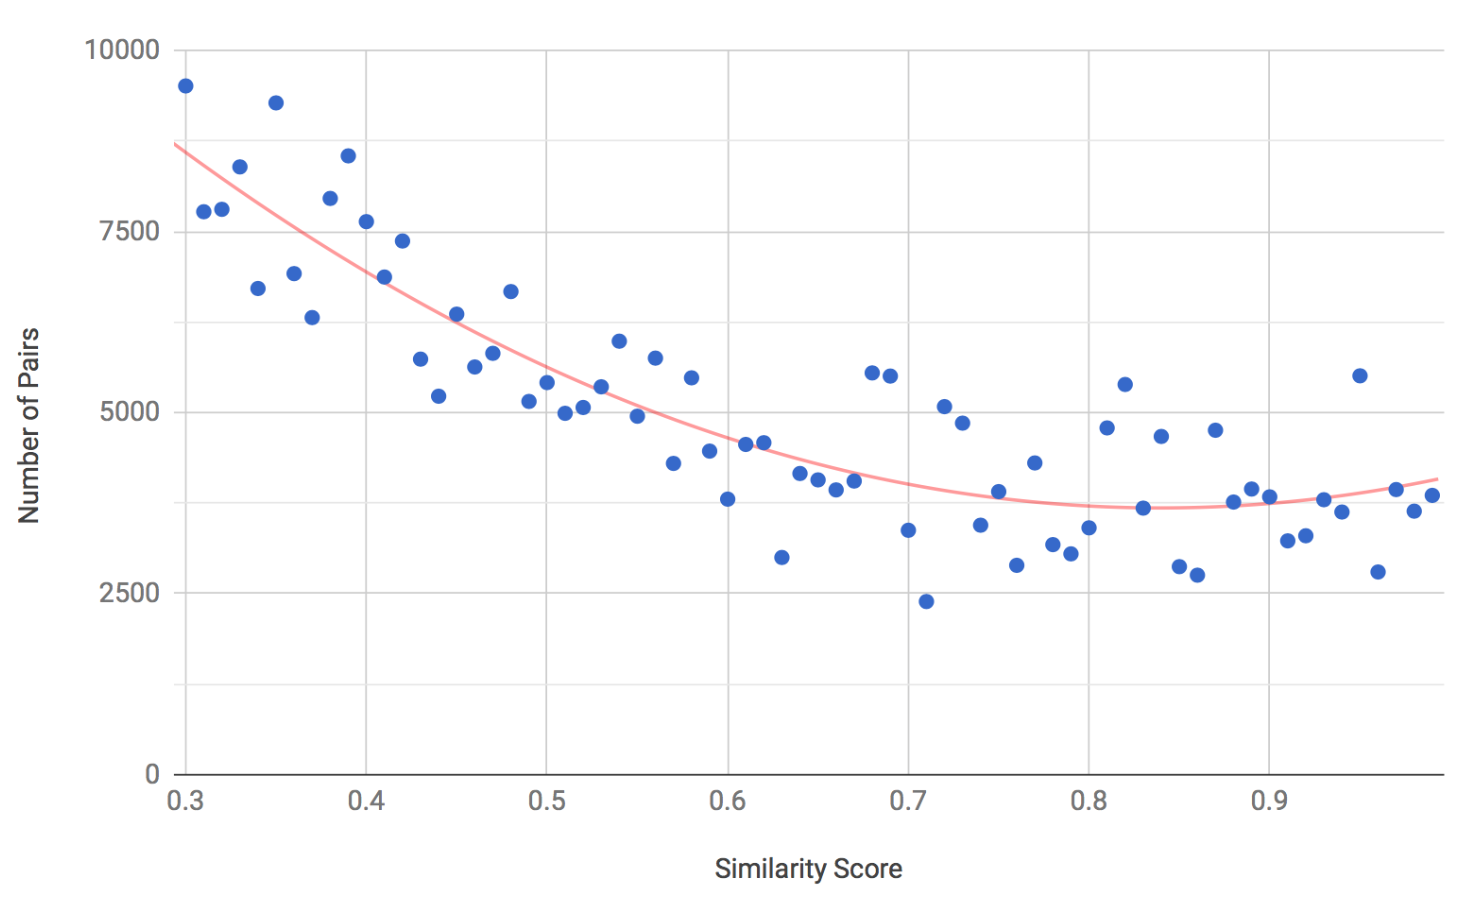
\includegraphics[scale=0.43]{similarity-threshold.png}
  \caption{Similarity values grouped by frequency in AIES}
  \label{fig:similarityThreshold}
\end{figure}

\subsubsection{Baselines}

We compare the performance of TDC, RDC and CRDC algorithms against the following baselines:
\begin{itemize}
  \item \textit{K-Means} as a centroid-based clustering approach.
  \item \textit{DBSCAN} as a density-based clustering approach.
  \item \textit{Random}, which randomly selects $R$ from the dataset
\end{itemize}

Initially, \textit{K-Means} \citep{Bahmani2012} randomly composes a set of centroids and assigns each point of the sample to its nearest cluster based on a distance measure. Then, a new set of centroids is calculated from the previous ones according to the assigned points. This process is repeated until the set of centroids does not change significantly between consecutive iterations or a maximum number of iterations is reached. The \textit{scalable K-Means} approach used in our experiments is an improved version of \textit{k-means} which obtains an initial set of centers ideally close to the optimum solution. The algorithm implemented at the Apache Commons Math library \footnote{ http://commons.apache.org/proper/commons-math/} was used in the experiments. Based on empirical results, the best configuration is: $k=number-of-topics=44$ and $maxIterations=50$

A widely known density-based algorithm is \textit{DBSCAN} \citep{Ester1996}, which compose clusters from the neighborhood of each point considering at least a minimum number of points and a given radius. Thus, it requires to specify the radius of the point's neighborhood, \textit{Eps}, and the minimum number of points in the neighborhood \textit{MinPts}. Based on empirical results, the best results were obtained with the following configuration: $eps=0.1$ and $minPts=50$

The \textit{Random} algorithm takes as input a parameter \textit{m} and randomly divides the dataset into \textit{m} equal-sized groups of similar documents. For the evaluation, $m$ was set to the number of topics, the dimension of the dataset.

With respect to the proposed algorithms and taking into account empirical results, the RDC algorithm is set to use the \textit{top1} highest topics, and the cumulative weight threshold for the CRDC algorithm is set to $0.9$.

\subsubsection{Measures}

A gold-standard is created for each dataset and distance metric considered. They are created by calculating all pairwise similarities from their documents. Since the $n \times n$ similarity matrix requires $O(n^2)$ time to be calculated, the selected size of datasets has not been too large $n=1000$.

We considered three measures to evaluate our algorithms with respect to the baseline:
\begin{itemize}
  \item \textbf{\textit{cost}}: based on the number of similarity score calculations required by the algorithm:
\begin{equation}
cost=(reqSim - minSim)/(totalSim - minSim)
\end{equation}
The \textit{minSim} corresponds to the number of similar documents obtained from using the \textit{threshold} score previously mentioned in section ~\ref{sec:clustering-threshold}. The \textit{totalSim} corresponds to the Cartesian product of existing documents: $totalSim=n*n=1,000,000$. And the \textit{reqSim} corresponds to the number of similarities calculated by the algorithm.
  \item \textbf{\textit{effectiveness}}: based on $precision$ and $recall$. It expresses the quality of the algorithm:
\begin{equation}
 effectiveness = \frac{precision^2  + recall^2}{2}
\end{equation}
  \item \textbf{\textit{efficiency}}: based on the previous ones, it express a compromise between quality and performance:
\begin{equation}
 efficiency = effectiveness - cost
\end{equation}
\end{itemize}

\subsubsection{Results}
\label{sec:clustering-results}

The source code used to evaluate the algorithms along with the results obtained are publicy available\footnote{https://doi.org/10.5281/zenodo.931305}.

In terms of \textbf{\textit{effectiveness}} (Figures ~\ref{fig:effectivenessJS} and ~\ref{fig:effectivenessHe}), the results highlight that \textit{K-Means} and \textit{CRDC} outperform the other algorithms. \textit{K-Means} was expected to be a top performer because the algorithm itself performs comparisons to map clusters. The fact that \textit{CRDC} has such good performance encourages us to think that, in fact, the most relevant topics when they altogether exceed a certain high weight threshold, are those that best represent the document and allow to group together similar documents. However, as shown in tables ~\ref{tab:precisionJS}, ~\ref{tab:precisionHe}, ~\ref{tab:recallJS} and ~\ref{tab:recallHe}, considering a fixed number of more relevant topics (\textit{RDC}) or considering the trend of their weights (\textit{TDC}) does not seem to perform so well on aggregating similar documents, since their \textit{precision} and \textit{recall} values are very low in both cases. It is surprising that the \textit{DBSCAN} has such low value. Taking a look at its \textit{precision} and \textit{recall} values, and also seeing the number of groups that each algorithm has created (Figure ~\ref{fig:clusters}), we believe that having a corpus containing a very cohesive set of documents (all papers in corpus belong to the same journal) affects the performance of this algorithm since it divides the corpus into a lower number of groups. This way, it obtains high values of \textit{recall} because most of the pair-wise distances are computed, but very low \textit{precision}.

The results also show that the behavior of the algorithms does not differ significantly when using different similarity measures, for example JS divergence (Figure ~\ref{fig:effectivenessJS}) and He distance (Figure ~\ref{fig:effectivenessHe}). This highlights the importance of the documents' topic distributions to successfully classify them into smaller groups of similar items, while other particular aspects such as the distance or similarity metric used to compare them are less influential.

\begin{figure}[!htb]\centering
  \center
  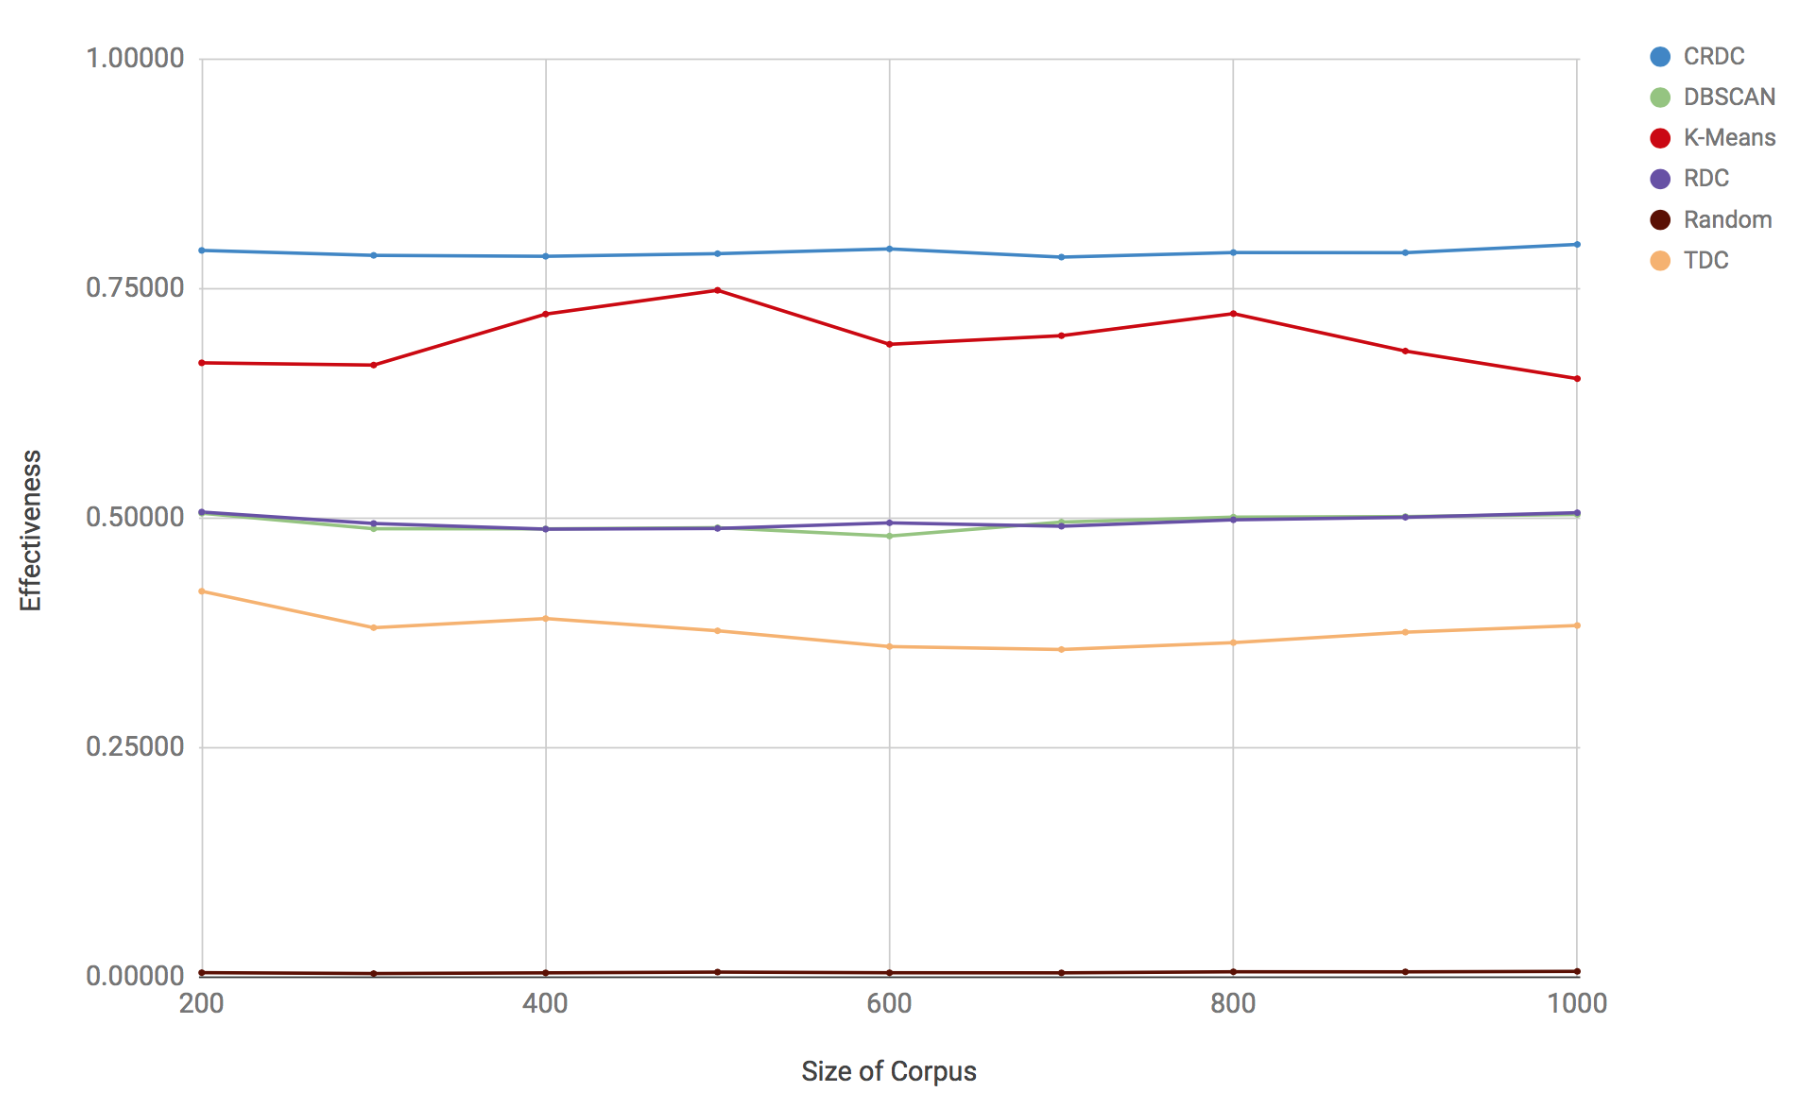
\includegraphics[scale=0.35]{effectivenessJS.png}
  \caption{Effectiveness (JS-based) in AIES}
  \label{fig:effectivenessJS}
\end{figure}

\begin{figure}[!htb]\centering
  \center
  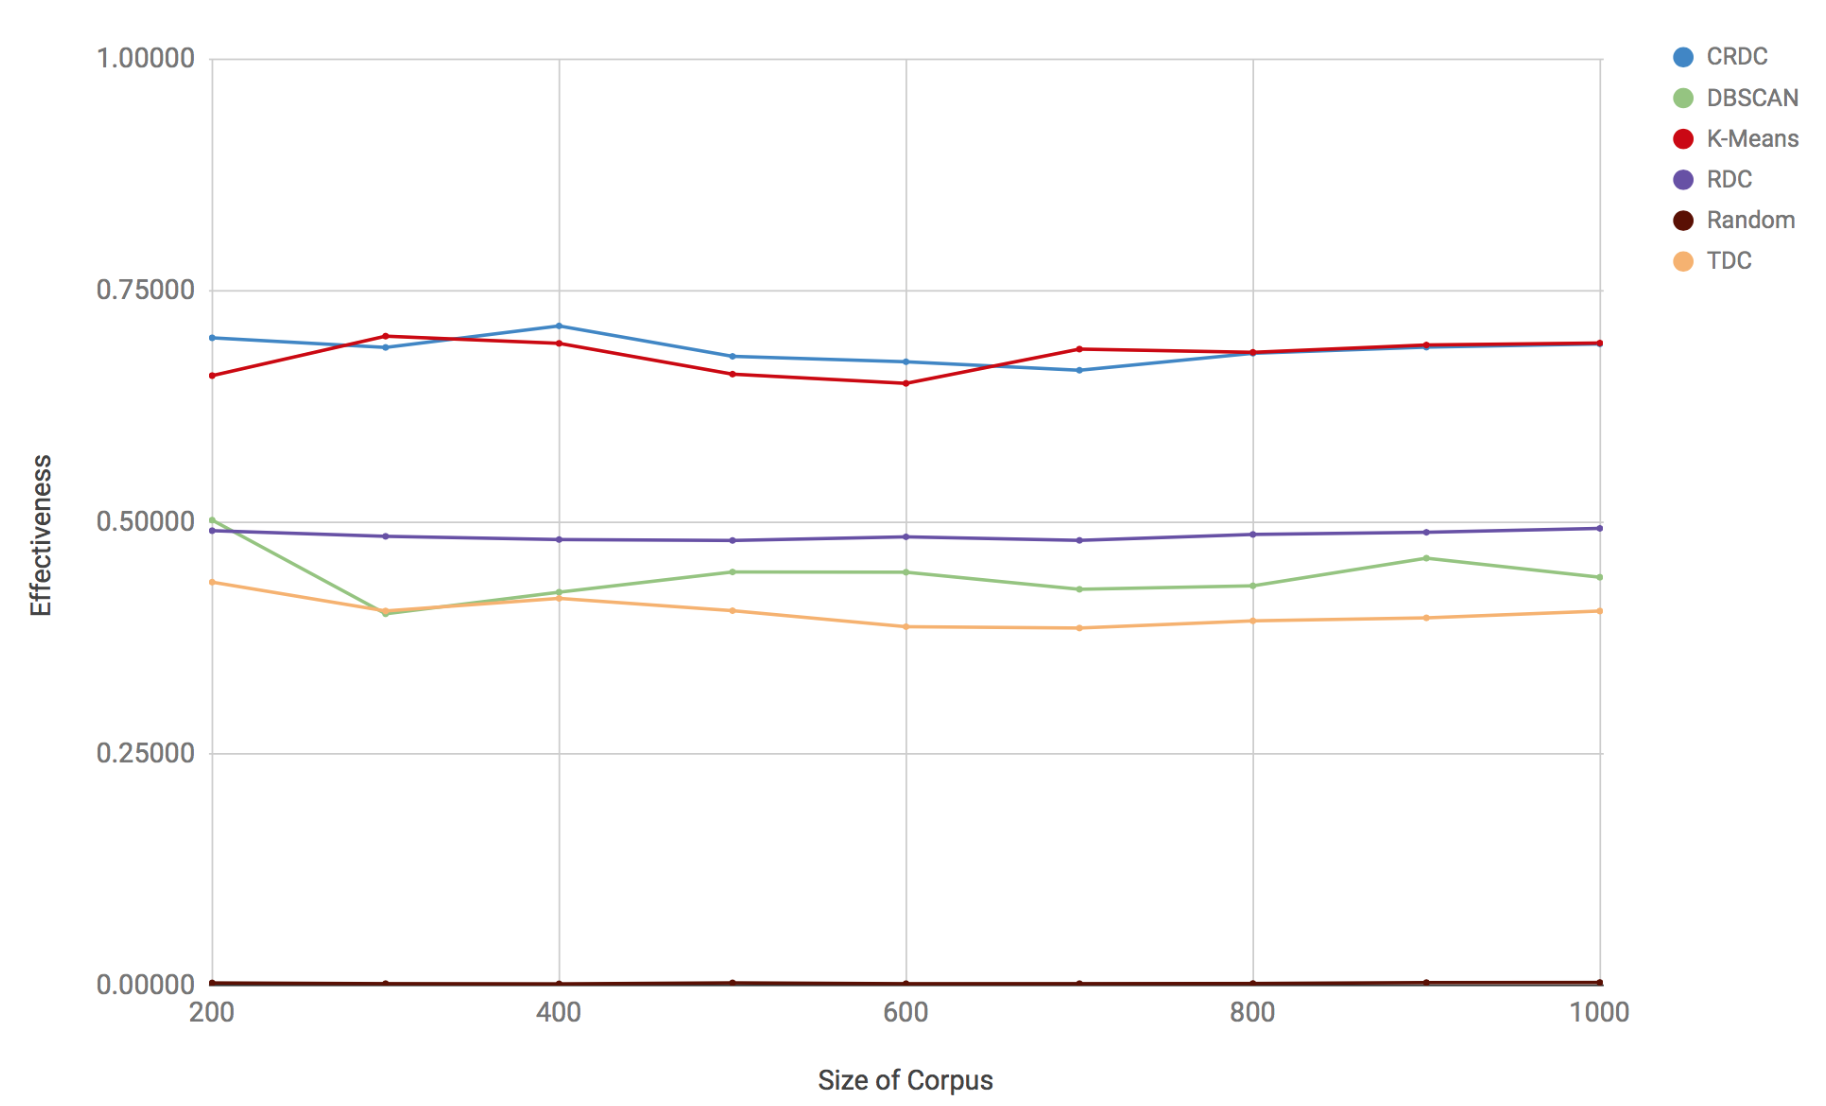
\includegraphics[scale=0.35]{effectivenessHe.png}
  \caption{Effectiveness (He-based) in AIES}
  \label{fig:effectivenessHe}
\end{figure}

\begin{figure}[!htb]\centering
  \center
  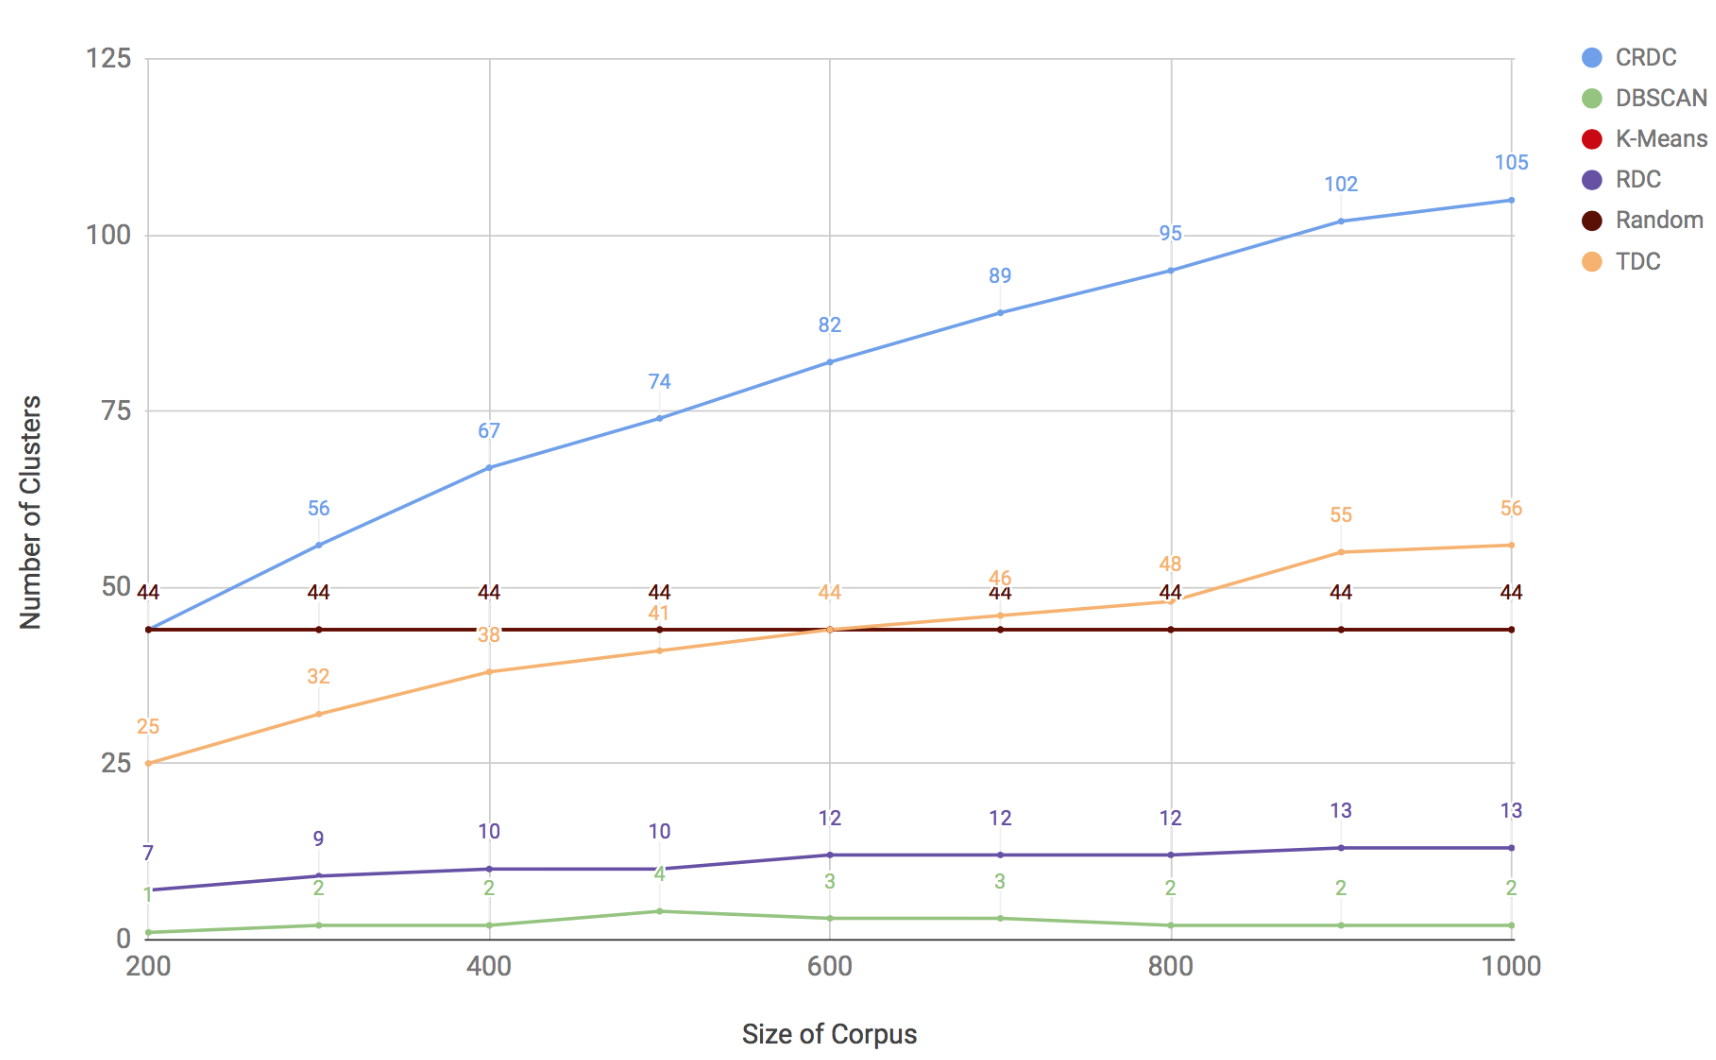
\includegraphics[scale=0.45]{clusters.png}
  \caption{Clusters in AIES}
  \label{fig:clusters}
\end{figure}

% table precision of algorithms
\begin{table}[!htb]
    \centering
        \begin{tabular}{l*{6}{c}r}\hline
                    Size    & CRDC & DBSCAN & K-Means & RDC & TDC  & Random \\
          \hline
					200 & 0.94 & 0.10 & \textbf{0.96} & 0.31 & 0.42 & 0.12 \\
					300 & 0.93 & 0.15 & \textbf{0.94} & 0.30 & 0.39 & 0.08 \\
					400 & \textbf{0.93} & 0.15 & 0.89 & 0.29 & 0.39 & 0.09 \\
					500 & \textbf{0.92} & 0.30 & 0.90 & 0.28 & 0.38 & 0.09 \\
					600 & \textbf{0.92} & 0.19 & 0.88 & 0.28 & 0.38 & 0.08 \\
					700 & \textbf{0.92} & 0.20 & 0.91 & 0.28 & 0.38 & 0.09 \\
					800 & \textbf{0.92} & 0.12 & 0.89 & 0.30 & 0.39 & 0.10 \\
					900 & \textbf{0.92} & 0.13 & 0.87 & 0.30 & 0.40 & 0.10 \\
					1000 & \textbf{0.93} & 0.13 & 0.90 & 0.30 & 0.40 & 0.10 \\
        \end{tabular}
    \caption{Precision (JS-based) in AIES}\label{tab:precisionJS}
\end{table}

\begin{table}[!htb]
    \centering
        \begin{tabular}{l*{6}{c}r}\hline
                    Size  & CRDC & DBSCAN & K-Means & RDC & TDC  & Random \\
          \hline
					200 & 0.75 & 0.07 & \textbf{0.84} & 0.23 & 0.08 & 0.33 \\
					300 & 0.74 & 0.08 & \textbf{0.83} & 0.23 & 0.06 & 0.32 \\
					400 & \textbf{0.76} & \textbf{0.09} & 0.76 & 0.22 & 0.06 & 0.32 \\
					500 & 0.73 & 0.08 & \textbf{0.74} & 0.21 & 0.08 & 0.31 \\
					600 & 0.72 & 0.08 & \textbf{0.73} & 0.21 & 0.06 & 0.30 \\
					700 & 0.71 & 0.10 & \textbf{0.76} & 0.21 & 0.06 & 0.30 \\
					800 & 0.73 & 0.11 & \textbf{0.78} & 0.22 & 0.07 & 0.31 \\
					900 & 0.73 & 0.12 & \textbf{0.80} & 0.22 & 0.08 & 0.32 \\
					1000 & 0.74 & 0.15 & \textbf{0.77} & 0.23 & 0.08 & 0.32 \\
        \end{tabular}
    \caption{Precision (He-based) in AIES}\label{tab:precisionHe}
\end{table}

% table recall of algorithms
\begin{table}[!htb]
    \centering
        \begin{tabular}{l*{6}{c}r}\hline
                    Size  & CRDC & DBSCAN & K-Means & RDC & TDC  & Random \\
          \hline
					200  & 0.92  & \textbf{1.00}  & 0.79  & 0.96  & 0.02  & 0.87 \\
					300  & 0.91  & 0.89  & 0.84  & \textbf{0.96}  & 0.02  & 0.84 \\
					400  & 0.92  & 0.92  & 0.90  & \textbf{0.96}  & 0.02  & 0.86 \\
					500  & 0.91  & 0.94  & 0.88  & \textbf{0.96}  & 0.03  & 0.85 \\
					600  & 0.91  & 0.94  & 0.87  & \textbf{0.96}  & 0.02  & 0.83 \\
					700  & 0.91  & 0.92  & 0.90  & \textbf{0.96}  & 0.02  & 0.83 \\
					800  & 0.92  & 0.92  & 0.88  & \textbf{0.96}  & 0.02  & 0.83 \\
					900  & 0.92  & 0.95  & 0.86  & \textbf{0.96}  & 0.02  & 0.83 \\
					1000  & 0.92  & 0.93  & 0.89  & \textbf{0.97}  & 0.02  & 0.84 \\
        \end{tabular}
    \caption{Recall (JS-based) in AIES}\label{tab:recallHe}
\end{table}

\begin{table}[!htb]
    \centering
        \begin{tabular}{l*{6}{c}r}\hline
                    Size`  & CRDC & DBSCAN & K-Means & RDC & TDC  & Random \\
          \hline
					200 & 0.84 & \textbf{1.00} & 0.65 & 0.96 & 0.02 & 0.82 \\
					300 & 0.84 & \textbf{0.98} & 0.76 & 0.95 & 0.02 & 0.78 \\
					400 & 0.84 & \textbf{0.98} & 0.79 & 0.94 & 0.02 & 0.79 \\
					500 & 0.85 & 0.94 & 0.87 & \textbf{0.95} & 0.02 & 0.78 \\
					600 & 0.86 & \textbf{0.96} & 0.80 & 0.95 & 0.02 & 0.76 \\
					700 & 0.85 & \textbf{0.98} & 0.80 & 0.95 & 0.02 & 0.76 \\
					800 & 0.85 & \textbf{0.99} & 0.81 & 0.95 & 0.02 & 0.76 \\
					900 & 0.85 & \textbf{0.99} & 0.75 & 0.95 & 0.02 & 0.77 \\
					1000 & 0.86 & \textbf{1.00} & 0.74 & 0.96 & 0.02 & 0.78 \\
        \end{tabular}
    \caption{Recall (He-based) in AIES}\label{tab:recallJS}
\end{table}



In terms of \textbf{\textit{cost}} (Figures ~\ref{fig:costJS} and ~\ref{fig:costHe}), the best clustering algorithm, as expected, is based on \textit{random} selection. This is due to the fact that the number of pairs compared by this algorithm is always the minimum, given the dataset is simply randomly divided into \textit{m} equal-sized groups, where \textit{m} is equals to the number of topics, i.e. dimension of the dataset. Since \textit{K-Means} and \textit{DBSCAN} make comparisons between documents until their internal condition is satisfied, they are the most inefficient approaches. \textit{K-Means} involves the highest cost because it compares all the documents with the 44 centroids in each iteration.

Among our proposals, the main reason for an algorithm to present a higher cost is due to the number of groups the corpus is divided into (see Figure ~\ref{fig:clusters}). The greater the number of groups, the fewer the number of later comparisons that have to be made and, therefore, the lower the cost of the algorithm.

The behavior of the \textit{DBSCAN} algorithm depends remarkably on the similarity metric used. We think that this may be due to the way in which both measures satisfy the triangle inequality condition, since one is based on divergence (JS) and the other on distance (He). This property, which defines $distance(a,b) \leq distance(a,c) + distance(c,b)$, is very important in the calculations that \textit{DBSCAN} makes to discover the groups, since it only calculates the distances between near points.

\begin{figure}[!htb]\centering
  \center
  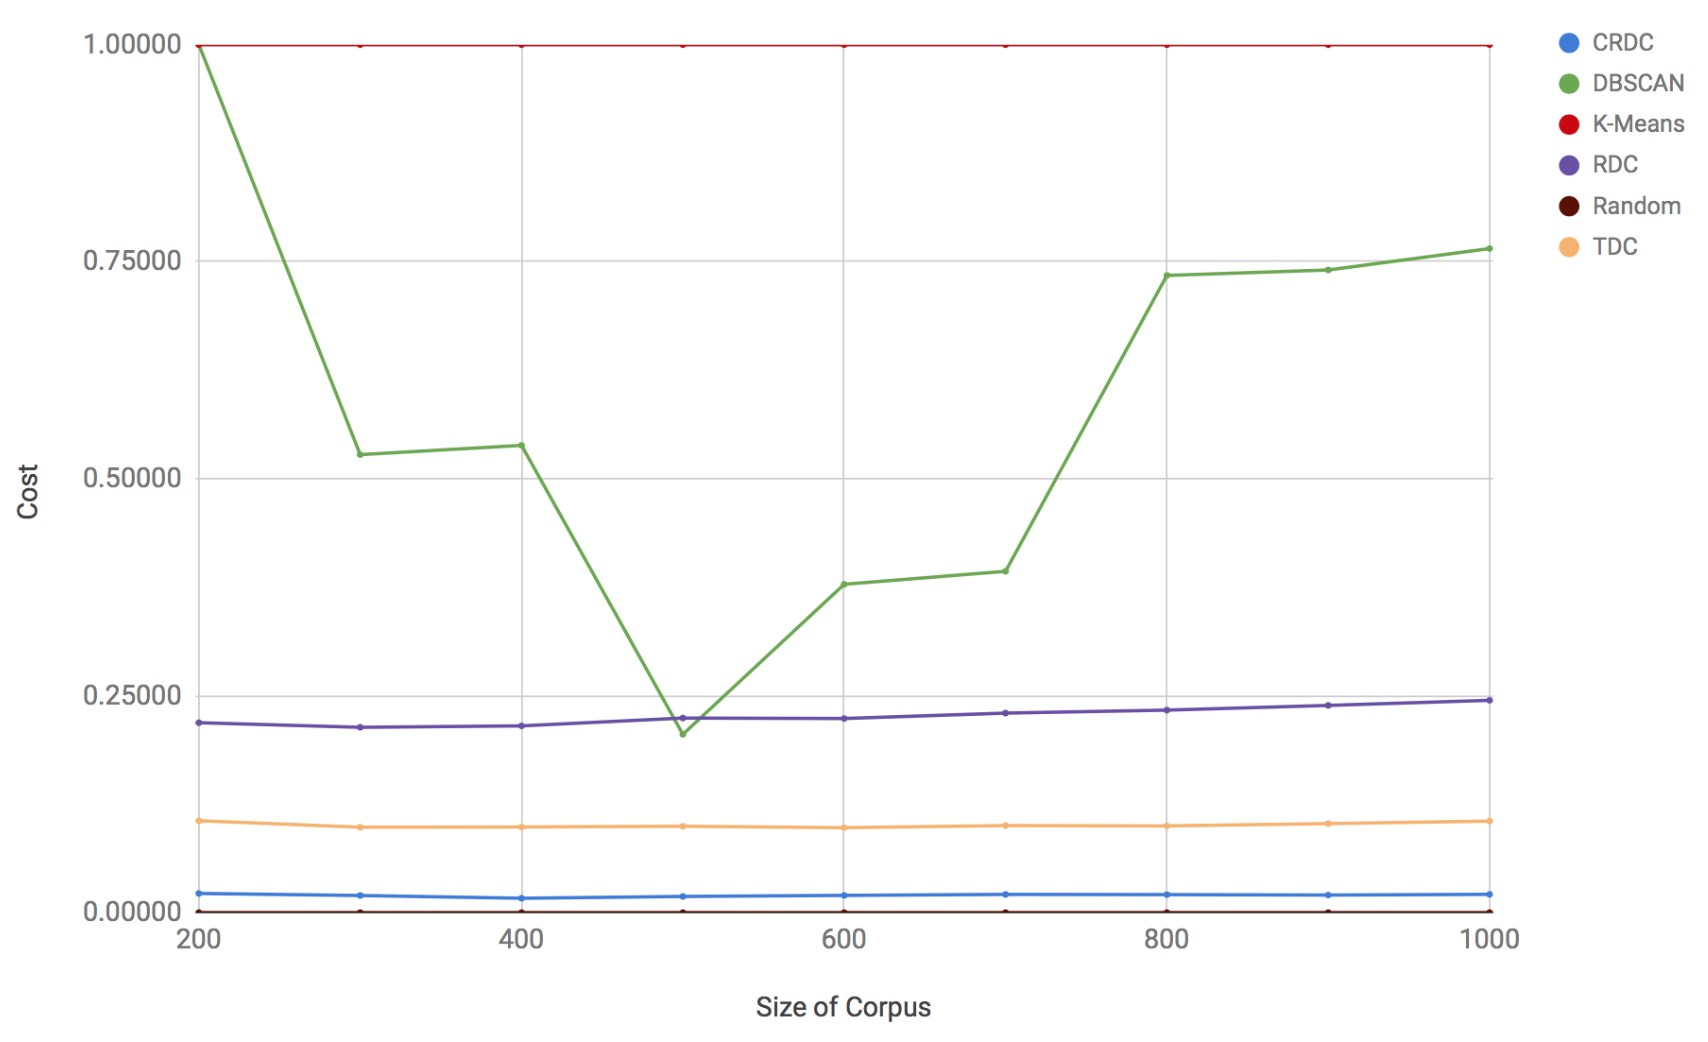
\includegraphics[scale=0.45]{costJS.png}
  \caption{Cost (JS-based) in AIES}
  \label{fig:costJS}
\end{figure}

\begin{figure}[!htb]\centering
  \center
  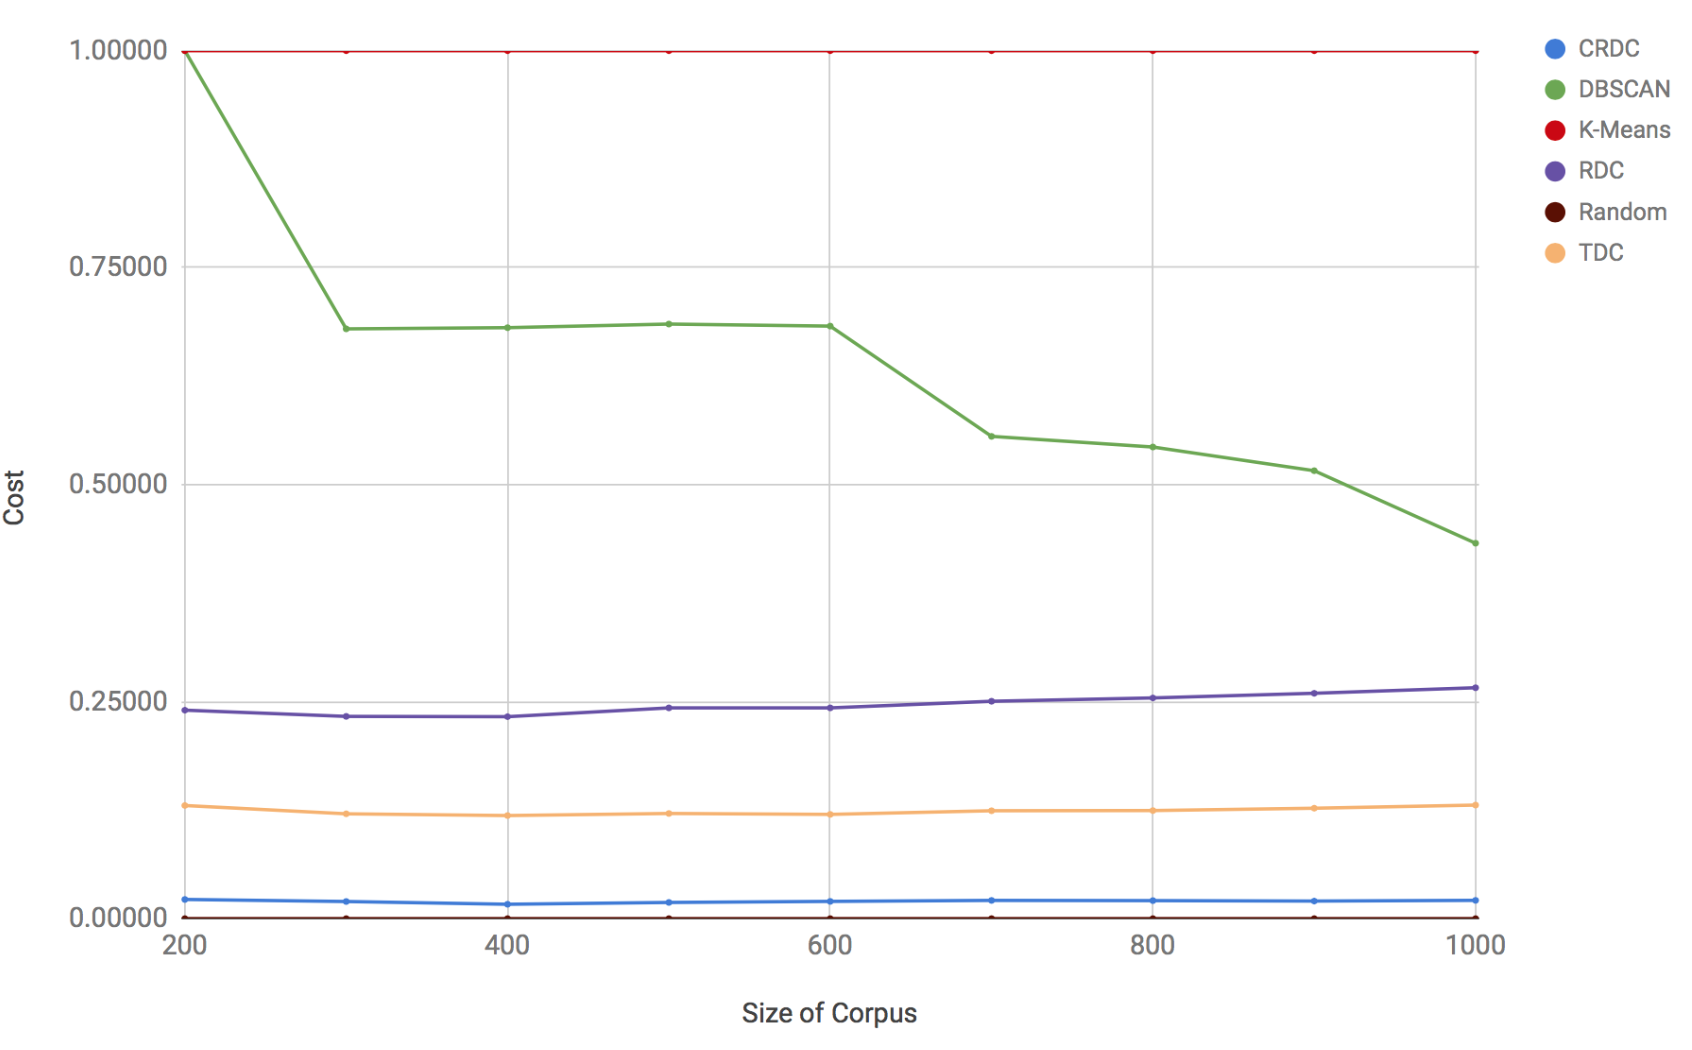
\includegraphics[scale=0.45]{costHe.png}
  \caption{Cost (He-based) in AIES}
  \label{fig:costHe}
\end{figure}

Finally, in terms of \textbf{\textit{efficiency}} (Figures ~\ref{fig:efficiencyJS}, ~\ref{fig:efficiencyHe}), regardless of the similarity measure used, the algorithm that yields the best performance according to the results obtained is \textit{CRDC}. Overall, \textit{CRDC} demonstrates a high accuracy classification and a lower cost by improving the performance offered by centroid-based or density-based approaches.

\begin{figure}[!htb]\centering
  \center
  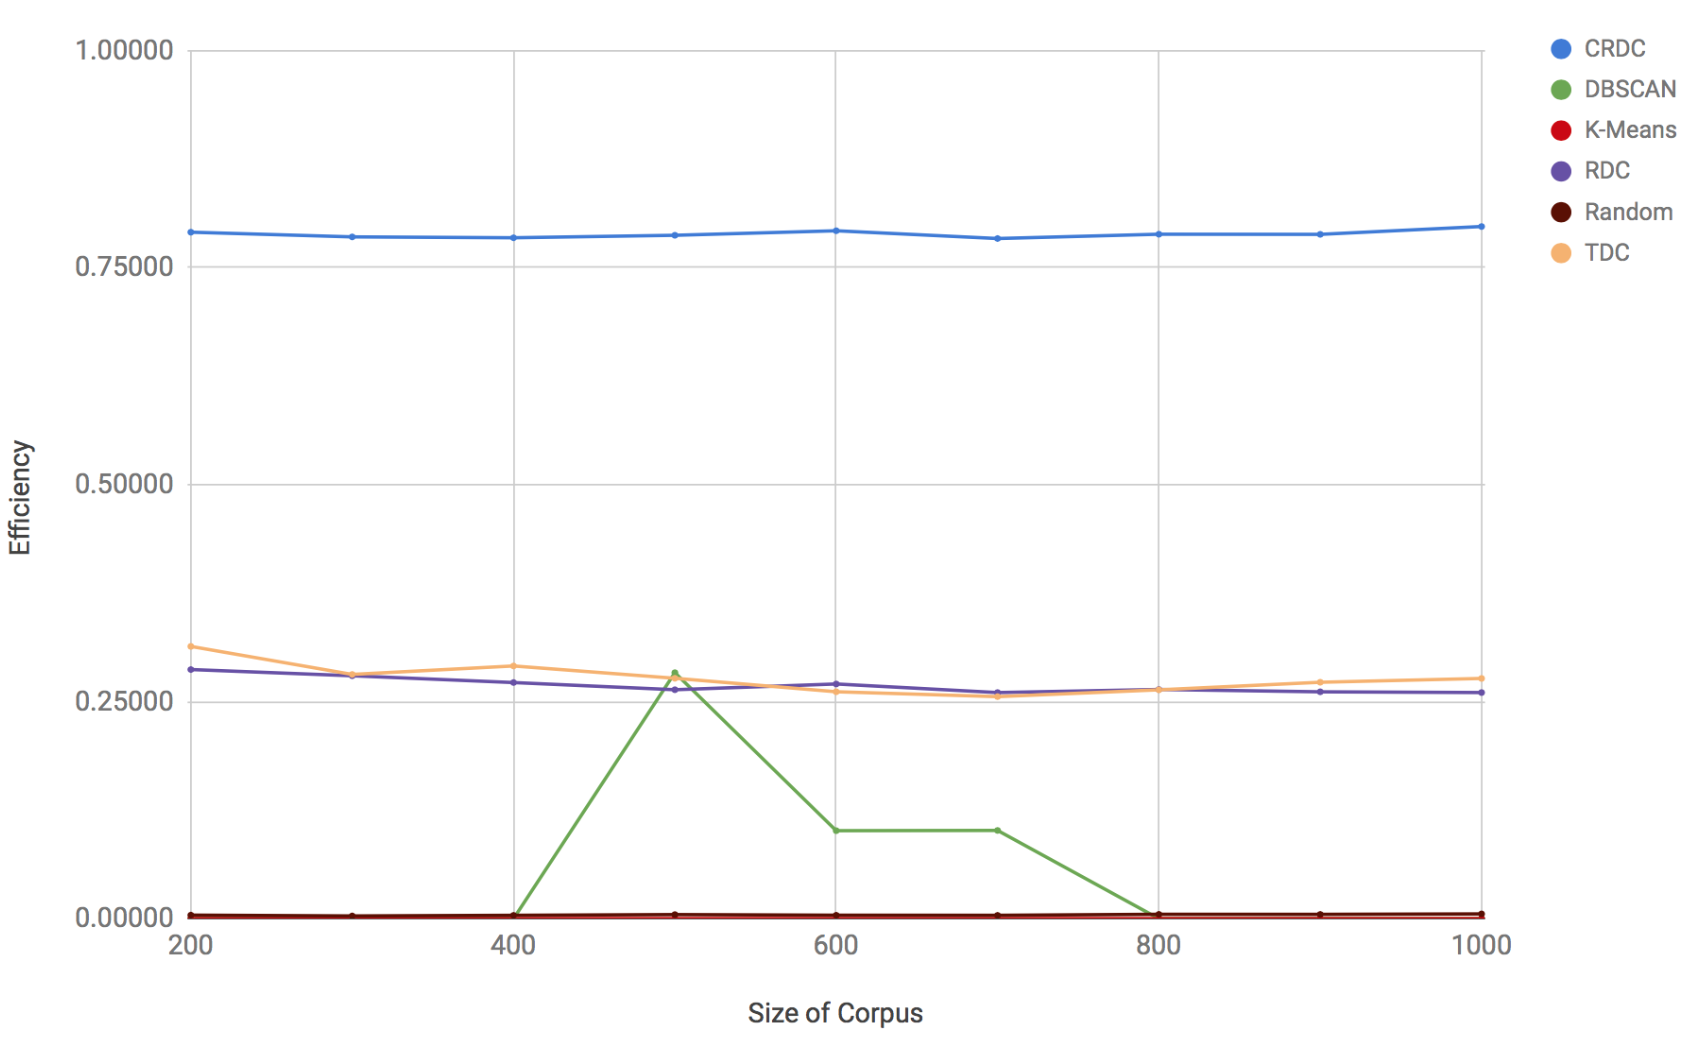
\includegraphics[scale=0.45]{efficiencyJS.png}
  \caption{Efficiency (JS-based) in AIES}
  \label{fig:efficiencyJS}
\end{figure}

\begin{figure}[!htb]\centering
  \center
  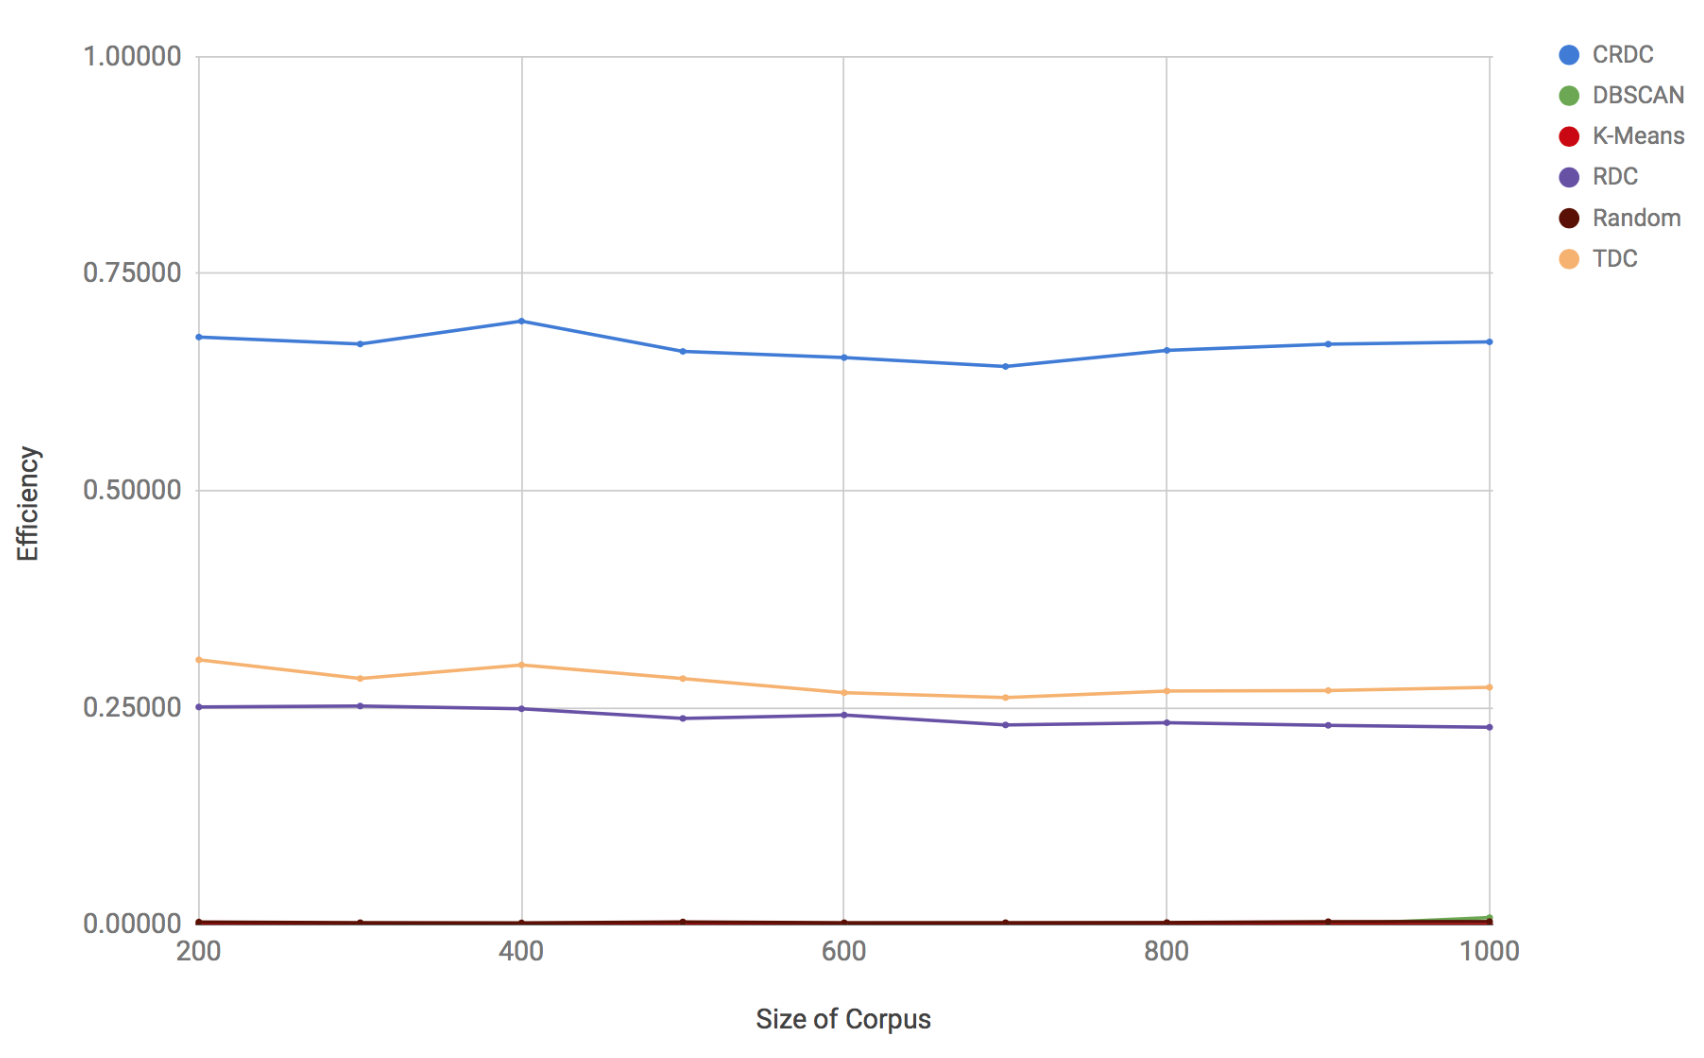
\includegraphics[scale=0.45]{efficiencyHe.png}
  \caption{Efficiency (He-based) in AIES}
  \label{fig:efficiencyHe}
\end{figure}

We have also created a synthetic dataset, DRM (Section ~\ref{sec:clustering-datasets}), composed of 1000 Dirichlet distributions with the same dimensions than topics in AIES: $k=44$. Unlike AIES, topic distributions have been randomly generated which imply that the similarity values are not so high: $min=0.06$, $mean=0.18$ and $max=0.61$. Following the same criteria than before (Section ~\ref{sec:clustering-threshold}), the similarity threshold is now fixed to 0.34 (Figure ~\ref{fig:similaritiesDRM}). Results \textbf{in terms of \textit{effectiveness}} (Figure ~\ref{fig:effectivenessDRMJS}) show a poor performance of the RDC and CRDC algorithms. The reason is that both are based on the fact that the highest weighted topics are shared between similar distributions. However, this condition is not satisfied when the similarity value between them is low.


\begin{figure}[!htb]\centering
  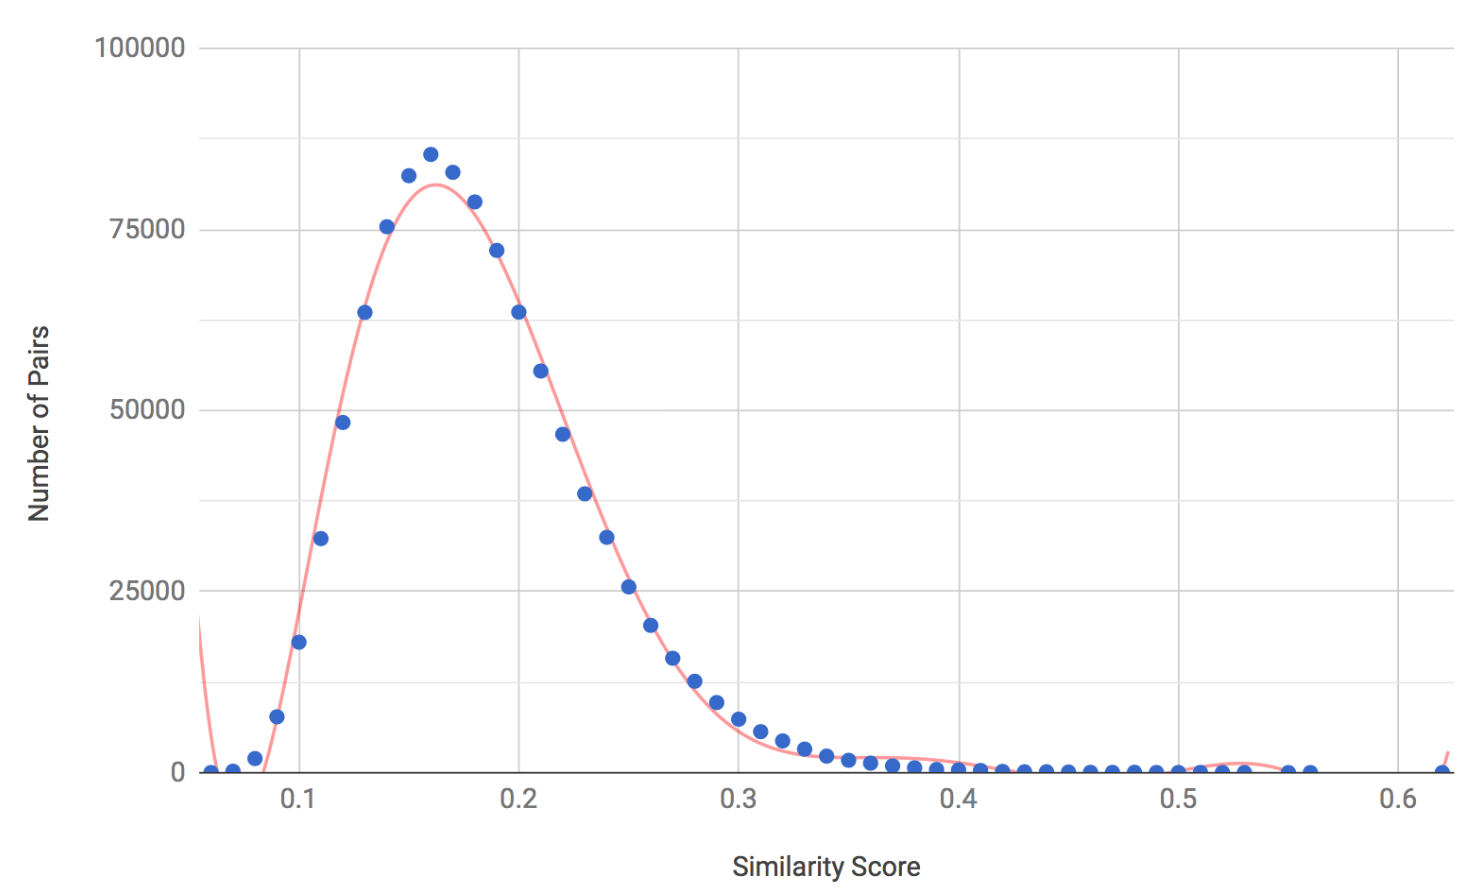
\includegraphics[scale=0.50]{similaritiesDRM.png}
  \caption{Similarity values grouped by frequency in DRM}
  \label{fig:similaritiesDRM}
\end{figure}


To confirm this behavior, we created a third dataset (DRM2) with the same size but with only 4 dimensions (4 topics). The goal is to achieve more similar distributions than in DRM even though they are also randomly generated. Since the similarity values range from $min=0.04$, $mean=0.34$ to $max=0.99$, the similarity threshold is now fixed to 0.66 (more details in section ~\ref{sec:clustering-threshold}). The results (Figure ~\ref{fig:effectivenessDRM2JS}) show an improvement in the accuracy of both the RDC and CRDC algorithms. Although scores are still not as high as for the AIES dataset, the increase compared to the DRM dataset shows that their \textit{precision} and \textit{recall} improve when the similarity threshold is higher. On the other hand, both the DBSCAN and TDC algorithms show similar behavior in both datasets, which means that their performance is not affected by the similarity threshold.

\subsection{Conclusion}
\label{sec:clustering-conclusion}

Processing a continuously growing collection of human generated documents requires techniques that divide the space into smaller regions containing potentially similar documents. Some algorithms in the literature tackle this problem from an unsupervised point of view, but they incur in high temporal costs and may not be suited for the domain being studied.

\begin{figure}[!htb]\centering
  \center
  \includegraphics[scale=0.45]{effectivenessDRMJS.png}
  \caption{Effectiveness (JS based) in DRM}
  \label{fig:effectivenessDRMJS}
\end{figure}

\begin{figure}[!htb]\centering
  \center
  \includegraphics[scale=0.45]{effectivenessDRM2JS.png}
  \caption{Effectiveness (JS based) in DRM2}
  \label{fig:effectivenessDRM2JS}
\end{figure}


%Present solution.
Three novel unsupervised clustering algorithms, \textit{TDC}, \textit{RDC} and \textit{CRDC}, are described in this section relying on the distributions inferred from a topic modeling algorithm (LDA). They are presented as a means to identify a smaller set of documents where only the similarity function has to be computed. They leverage on the particular behavior of Dirichlet distributions describing topic distributions, where the highest weighted topics have a high influence on the rest of topics. This also means that given a topic distribution, the relations between their topic weights such as order or trends between them, are more important than the density values.

Although we initially thought that using only a fixed number of topics with higher weights of a topic distribution (\textit{RDC}), or taking into account only the trend changes between the weights of consecutive topics (\textit{TDC}), could be enough to classify similar topic distributions, the results obtained have shown that these properties are not sufficient. Results in terms of \textit{efficiency}, \textit{effectiveness} and \textit{cost} have been shown comparing the proposed algorithms with existing centroid-based and density-based clustering techniques. They reveal that obtaining the most representative topics of a topic distribution  by comparing the sum of their weights with respect to the rest (\textit{CRDC}) is a promising approach, which improves the \textit{efficiency} obtained by other centroid-based and density-based approaches. While \textit{K-Means} takes $O(n^k * \log{n})$ and \textit{DBSCAN} takes $O(n * \log{n})$ time to classify $n$ documents in a collection, the proposed algorithms only take linear time ($O(n)$) because they do not require any other data except their own topic distribution to assign it to a cluster.


\section{Summary}

In Section \ref{sec:topic-relations}, we have analyzed the representativeness of topics to describe texts, using the particular case of scientific articles. Our experiment with a corpus of research papers published in the \textit{Advances in Engineering Software} (AIES) journal shows that abstracts are not sufficiently representative to describe, by means of topics, the content of a paper. This behavior suggests that texts with greater vocabulary that emphasize key terms through repetition, favor topic-based representation. Therefore, if we want to construct a system that relates scientific articles, it would be better to use full texts rather than abstracts, as it is done by many more traditional techniques. This has a higher computational cost, for which systems like \textit{librAIry} behave sufficiently well.

Taking into account the relevance of topics to describe texts, we analyze in Section {\ref{sec:topic-clustering}} the behavior of topic distributions to calculate distances between documents using topic models with different dimensions. By using clustering techniques at the topic level, the most representative topics of a topic distribution are identified regardless of the number of dimensions that the model has. A topic-based representation is then proposed that covers the third research objective of this thesis (R03, \textit{define annotations based on topics that enable a semantic-aware exploration of the knowledge inside a corpus}). 

A new distance metric is also proposed that takes advantage of such representation to compare documents. Its performance is analyzed by automatically clustering the JRC-Acquis corpus according to EUROVOC categories. Tables \ref{tab:precisionHe}, \ref{tab:precisionJS}, \ref{tab:recallHe} and \ref{tab:recallJS} show results with high precision and recall in unsupervised classification tasks. This new way of relating documents from their most representative topics covers the fourth research objective of this thesis (R04, \textit{define a metric based on topic annotations that compares documents and facilitates their interpretation}). 

In order to perform the experiments, both the representation based on the most relevant topics and the distance metric based on these representations have been implemented in \textit{librAIry}. This partially covers the third and fourth technical objectives (T03, \textit{integrate the annotation method base on topic hierarchies into the topic model service}) (T04, \textit{create a system capable of finding similar document automatically}).

% this file is called up by thesis.tex
% content in this file will be fed into the main document

%: ----------------------- introduction file header -----------------------
\chapter{Large-scale Comparisons of Topic Distributions}\label{ch:comparisons}

\graphicspath{{comparisons/figures/}}

% -------------------------------------------------------------
% -- Comparisons
% -------------------------------------------------------------

As we showed in Section \ref{sec:topic-clustering}, grouping topics by a cumulative ranking is a useful mechanism for simplifying representations based on topic distributions. Relevant topics emerge as those whose accumulated weight exceeds a threshold, after ordering all topics and starting from the top. This technique has shown a promising performance to cluster documents ( Section \ref{sec:clustering-results}) and  suggests that \textit{similar documents share the most relevant topics}. However, the approach still has limitations: it depends on the manual tuning of a parameter, the threshold; and it does not measure degrees of similarity since it only establishes whether or not two documents are similar. As shown in Chapter \ref{ch:hypothesis}, we hypothesize that is possible to find relevant documents with similar topic distributions without calculating all pairwise comparisons and without discarding the notion of topics from their representation. In this chapter we introduce relevance levels between topics and present our approach to compare documents from huge collections through hierarchical representations of their topic distributions \citep{Badenes-Olmedo2019}.

\section{Hashing Topic Distributions}
\label{sec:comparison-hashing}

One of the greatest advantages of using Probabilistic Topic Models (PTM) in large document collections is the ability to represent documents as probability distributions over a small number of topics, thereby mapping documents into a low-dimensional latent space (the K-dimensional probability simplex, where K is the number of topics). A document, represented as a point in this simplex, is said to have a particular topic distribution. As seen in Section \ref{sec:topic-clustering}, the low-dimensional feature space created by topic models could also be suitable for document similarity tasks, especially on big real-world data sets, since topic distributions are continuous and not as sparse as discrete-term feature vectors and can be explained in terms of relevance. 

Hashing methods transform the data points from the original feature space into a binary-code Hamming space, where the similarities in the original space are preserved. They can learn hash functions (data-dependent) or use projections (data-independent) from the training data \cite{Wang2016}. Data-independent methods unlike data-dependent ones do not need to be re-calculated when data changes, i.e. adding or removing documents to the collection. Taking large-scale scenarios into account (e.g. Document clustering, Content-based Recommendation, Duplicate Detection), this is a key feature along with the ability to infer hash codes individually (for each document) rather than on a set of documents. 

Data-independent hashing methods depend on two key elements: (1) data type and (2) distance metric. For vector-type data, as introduced in Section \ref{sec:related-work}, based on $l_p$ distance with $p \epsilon [0,2)$ lots of hashing methods have been proposed, such as p-stable Locality-Sensitive Hashing (LSH) \citep{Datar2004}, Leech lattice LSH \citep{Andoni2006}, Spherical LSH \citep{Terasawa2007}, and Beyond LSH \citep{Andoni2014}. Based on the $\theta$ distance many methods have been developed such as Kernel LSH \citep{Kulis2012} and Hyperplane hashing \citep{Vijayanarasimhan2014}. But only few methods handle density metrics in a simplex space. A first approach transformed the $He$ divergence into an Euclidean distance so that existing ANN techniques, such as LSH and k-d tree, could be applied \citep{Krstovski2013a}. But this solution does not consider the special attributions of probability distributions, such as Non-negative and Sum-equal-one. Recently, a hashing schema \citep{Mao2017} taking into account the symmetry has been proposed, non-negativity and triangle inequality features of the S2JSD metric for probability distributions. For set-type data, Jaccard Coefficient is the main metric used. Some examples are K-min Sketch \citep{Li2012}, Min-max hash \citep{Ji2013}, B-bit minwise hashing \citep{Li2010b} and Sim-min-hash \citep{Zhao2013}.

All of them have demonstrated efficiency in the search for similar documents, but none of them allows the search for documents (1) by thematic areas or (2) by similarity levels, nor they offer (3) an explanation about the similarity obtained beyond the vectors used to calculate it. Binary-hash codes drop a very precious information: the topic relevance.

A new hierarchical set-type data is proposed (Figure \ref{fig:hash_functions}). Each level of the hierarchy indicates the importance of the topic according to its distribution. Level 0 contains the topics with the highest score. Level 1 contains the topics with highest score once the first ones have been eliminated, and so on. From a vector of components, where each of the components is the score of topic $t$, a  vector containing set of topics is proposed, where each of the dimensions means a topic relevance. Thus, for the topic distribution
$q=[0.02,0.14,0.02,0.16,0.04,0.09,0.19,0.12,0.04,0.17]$, a hierarchical set of topics may be $h=\left \{(t6),(t9,t3),(t1) \right \}$. It means that topic $t6$ (0.19) is the most relevant, then topics $t9$ (0.17) and $t3$ (0.16) and, finally, topic $t1$ (0.14). This is just an example about the data structure that will support the different hashing strategies. In Section \ref{sec:comparison-hash} some approaches to create hash codes based on this data structure are described.

\begin{figure*}
\includegraphics[width=\textwidth,height=9cm]{hashFunctions.png}
\caption{Hash method based on hierarchical set of topics from a given topic distribution}
\label{fig:hash_functions}
\end{figure*}

\subsection{Data Type}
\label{sec:comparison-datatype}
As seen in Section \ref{sec:related-work}, a traditional approach to text representation usually requires encoding of documents into numerical vectors. Words are extracted from a corpus as feature candidates and based on a certain criterion they are assigned values to describe the documents: term-frequency, TF-IDF, information gain, and chi-square are typical measures. But this causes two main problems: huge number of dimensions and sparse distribution. The use of topics as feature space has been extended to mapping documents into low-dimensional vectors. However, as shown in Figure \ref{fig:topic_distances}, the distance metrics based on probability densities vary according to the dimensions of the model and reveal the difficulty of calculating the similarity values using the vectors with the topic distributions.  

Since hashing techniques can transform both vector and set-based data \citep{Mao2017, Ji2013} into a new space where the similarity (i.e. closeness of points) in the original feature space is preserved, a new set-based data structure is proposed in this paper. It is created from clusters of topics organized by relevance levels and it aims to extend the ability of building queries with topic-based restrictions over the searching space while maintaining high level of accuracy.

The new hierarchical set-type data describes each document as a sequence of sets of topics sorted by relevance. Each level of the hierarchy expresses how important those topics are in that document. In the first level (i.e level 0) are the topics with the highest score. In the second level (i.e level 1) are the topics with the highest score once the first ones have been removed, and so on. In this work, several clustering approaches have been considered to assign topics to each level.

In a feature space created from a PTM with eight topics, for example, each data point $p$ is described by a eight-dimensional vector with the topic distributions: $vp=[t0,t1,t2,t3,t4,t5,t6,t7]$ . Then, given a point $q1=[0.18, 0.15, 0.2, 0.05, 0.14, 0.11, 0.09, 0.08]$, the three-level hierarchical set of topics may be $h=[\{t2\},\{t0\},\{t1,t4\}]$. It means that $t2$ is the most relevant topic, then topic $t0$ and finally topics $t1$ and $t4$. This is just an example about the data structure that will support the hashing strategies. In section \ref{sec:comparison-hash} some approaches to create hash codes based on this data structure are described.

Domain-specific features such as vocabulary, writing style, or speech type, have a major influence on the topic models, but not in the hashing algorithms described in this article. The methods for creating hash codes are agnostic of these particularities since they are only based on the topic distributions generated by the models. 

\subsection{Distance Metric}
Since documents are described by set-type data, the proposed distance metric is based on the Jaccard coefficient. This metric computes the similarity of sets by looking at the relative size of their intersection as follows:

%Jaccard Coefficient formula
\begin{equation}
J(A,B) = \frac{ | A \cap B |}{ | A \cup B |}
\label{eq:jc}
\end{equation}
where A and B are set of topics. 

More specifically, $d_J$ is based on the Jaccard distance, which is obtained by subtracting the Jaccard coefficient $J$ from 1:
%Jaccard distance formula
\begin{equation}
d_J(A,B) = 1 - J(A,B)
\label{eq:dj}
\end{equation}

The proposed distance measure $d_H$ used to compare hash codes created from set of topics is the sum of the Jaccard distances $d_j$ for each hierarchy level, i.e. for each set of topics:

%distance metric formula
\begin{equation}
d_H(H_1,H_2) = \sum\limits_{l=1}^L \Big( d_J(H_1(x_l),H_2(x_l)) \Big)
\label{eq:dh}
\end{equation}

where $H_1$ and $H_2$ are hash codes, $H_1(x_l)$ and $H_2(x_l)$ are the set of topics up to level $l$ for each hash code $H$ and $L$ is the maximum hierarchy level. A corner case is $L=T$, where $T$ is the number of topics in the model. 


\subsection{Hash Function}
\label{sec:comparison-hash}

The hash function clusters topics based on relevance levels. Three approaches are proposed depending on the criteria used to group topics: threshold-based, centroid-based and density-based.

\subsubsection{Threshold-based Hierarchical Hashing Method}
\label{sec:comparison-threshold}
This approach is just an initial and naive way of grouping topics by threshold values into each relevance level. They can be manually defined or automatically generated by thresholds dividing the topic distributions as follows:

%threshold formula
\begin{equation}
th_{inc} = \frac{1}{(L+1) \cdot T}
\label{eq:th}
\end{equation}
where $L$ is the number of hierarchy levels, and $T$ the number of topics.

\begin{figure}[t]\centering
\includegraphics[scale=0.35]{threshold-hash.png}
\caption{Threshold-based Hierarchical Hash (L=3)}
\label{fig:th_hash}
\end{figure}

If $L=3$ and $T=10$ for a topic distribution $td$ defined as follows:
%distance metric formula
\begin{equation}
    \begin{gathered}
td=[0.017, 0.141, 0.010, 0.172, 0.030, \\
0.090, 0.199,  0.133,  0.031, 0.171]
    \end{gathered}
    \label{eq:sample}
\end{equation}

Then, a threshold-based hierarchical hash $H_{T}$, with an automatically created threshold defined by equation \ref{eq:th}, is equals to $H_{T}=\{(t1,t3,t5,t6,t7,t9),(),(t4,t8)\}$ with $th_{inc}=0.025$ (Fig  \ref{fig:th_hash}).

\subsubsection{Centroid-based Hierarchical Hashing Method}
\label{sec:comparison-centroid}
This approach assumes topic distributions can be partitioned into $k$ clusters where each topic belongs to the cluster with the nearest mean score. It is based on the k-Means clustering algorithm, where $k$ is obtained by adding 1 to the number of hierarchy levels. Unlike the previous method, threshold values used to define the hierarchy levels may vary between documents, i.e. for each topic distribution, since they are calculated for each distribution separately.

\begin{figure}[t]\centering
\includegraphics[scale=0.35]{centroid-hash.png}
\caption{Centroid-based Hierarchical Hash (L=3)}
\label{fig:centroid_hash}
\end{figure}

Following the previous example, if $L=3$ and $T=10$ for a topic distribution $td$ defined in equation \ref{eq:sample}, then a centroid-based hieararchical hash $H_{C}$ equals to $H_{C}=\{(t6),(t9,t7,t3,t1),(t5)\}$ (Fig \ref{fig:centroid_hash}).


\subsubsection{Density-based Hierarchical Hashing Method}
\label{sec:comparison-density}
This approach also considers relative hierarchical thresholds for each relevance level. Now, a topic distribution is described by points in a single dimension. In this space, topics closely packed together are grouped together. This approach does not require a fixed number of groups. It only requires a maximum distance ($eps$) to consider two points close and grouped together. This value can be estimated from the own distribution of topics (e.g. variance).

\begin{figure}[t]\centering
\includegraphics[scale=0.35]{density-hash.png}
\caption{Density-based Hierarchical Hash (L=3)}
\label{fig:density_hash}
\end{figure}

Following the above example, if $L=3$ and $td$ is the topic distribution defined in equation \ref{eq:sample}, then a density-based hierarchical hash $H_{D}$ is equals to $H_{D}=\{(t6),(t9,t3),(t1)\}$ when $eps$ equals to the variance of the topic distribution (Fig \ref{fig:density_hash}).


\subsection{Online-mode Hashing}
\label{sec:comparison-onlineHashing}

Hashing methods are batch-mode learning models that require huge data for learning an optimal model and cannot handle unseen data. Recent work address online mode by learning algorithms \citep{Huang2018} that get hashing model accommodate to each new pair of data. But these approaches require the hashing model to be updated during each round based on the new pairs of data.

Our methods rely on topic models to build hash codes. These models do not require to be updated to make inferences about data not seen during training. In this way, the proposed hashing algorithms can work on large-scale and real-time data, as the size and the novelty of the collection does not influence the annotation process.

\section{Evaluation}
\label{sec:comparison-experiments}

As mentioned in Section \ref{sec:topic-explainability}, it is difficult to interpret the similarity score calculated by metrics in a probability space. Since all of them are based on adding the distance between each dimension of the model (eq. \ref{eq:kl}, \ref{eq:jsdivergence} and \ref{eq:hedistance}), distributions that share a fair amount of the less representative topics may still get higher similarity values than those that share the most representative ones specially if the model has a high number of dimensions.

\begin{figure}[!htb]\centering
   \begin{minipage}{0.49\textwidth}
     \frame{\includegraphics[width=\linewidth]{doc-similarity-pair1.png}}
     \caption{Topic Distribution of two documents with similarity score, based on JSD, equals to 0.74}\label{fig:doc_sim_1}
   \end{minipage}
   \begin {minipage}[c]{0.49\textwidth}
     \frame{\includegraphics[width=\linewidth]{doc-similarity-pair2.png}}
     \caption{Topic Distribution of two documents with similarity score, based on JSD, equals to 0.71}\label{fig:doc_sim_2}
   \end{minipage}
\end{figure}

Figures \ref{fig:doc_sim_1} and \ref{fig:doc_sim_2} show overlapped topic distributions of two pairs of documents. In the first case (fig  \ref{fig:doc_sim_1}), none of the most representative topics of each document is shared between them. However, the similarity score calculated from divergence-based metrics (eq \ref{eq:jsdivergence}) is higher than in the second case (fig  \ref{fig:doc_sim_2}), where the most representative topic is shared (topic 26). This behavior is due to the sum of the distances between the less representative topics (i.e. topics with a low weight value) being greater than the sum of the distances between the most representative ones (i.e. topic with a high weight value). In high-dimensional models, that sum may be more representative than the one obtained with the most relevant topics, which are fewer in number than the less relevant ones. 

The following experiments aim to validate that \textit{\textbf{hash codes based on hierarchical set of topics not only make it possible to search for similar documents with high accuracy, but also to extend queries with new restrictions and to offer information that helps explaining why two documents are similar}}.

\subsection{Datasets and Evaluation Metrics}
\label{sec:comparison-datasets}
Three datasets \citep{Badenes-Olmedo2019a} are used to validate the proposed approach. The OPEN-RESEARCH\footnote{https://labs.semanticscholar.org/corpus/} dataset consist of 500k research papers in Computer Science, Neuroscience, and Biomedical randomly selected from the Open Research Corpus \citep{Waleed2018}. The CORDIS\footnote{https://data.europa.eu/euodp/data/dataset/cordisref-data} dataset contains 100k documents describing research and innovation projects funded by the European Union under a framework programme since 1990. The PATENTS dataset consists of 1M patents randomly selected from the USPTO\footnote{https://www.uspto.gov/learning-and-resources/ip-policy/economic-research/research-datasets} collection. For each dataset, documents are mapped to two latent topic spaces with different dimensions using LDA. We perform parameter estimation using collapsed Gibbs sampling for LDA \citep{Griffiths2004b} from our librAIry  framework. The number of topics varies to study their influence on the performance of the algorithm (i.e. CORDIS-70 indicates a latent space created with 70 topics). 

Experiments use JS divergence as an information-theoretically motivated metric in the probabilistic space created by topic models. Since it is a smoothed and symmetric alternative to the KL divergence, which is a standard measure for comparing distributions \citep{Cha2007}, it has been extensively used as state-of-the-art metric over topic distributions in literature \citep{Towne2016, Aletras2017, Mao2017}. Our upper bound is created from the brute-force comparison of the reference documents with all documents in the collection to obtain the list of similar documents.  

In this scenario the goal is to minimize the accuracy loss introduced by hashing algorithms. Since this is a large-scale problem and an accuracy-oriented task, recall is not a good measure to be considered and precision is only relevant for sets much smaller than the total size of data (between 3-5 candidates).

All the experimental results are averaged over random training/set partitions. For each topic space, 100 documents are selected as references, and the remaining documents as search space. As noted above, only p@5 will be used to report the results of the experiments.

\subsection{Retrieving Similar Documents}
\label{sec:comparison-search}

It is challenging to create an exhaustive gold standard, given the significant amount of human labour that is required to get a comprehensive view of the subjects being covered in it. In order to overcome this problem, the list of similar documents to a given one is obtained after comparing the document with all the documents of the repository and sorting the result. We have observed that different distance functions perform similarly in this scenario (Fig. \ref{fig:topic_distances}), so we have decided to use only the JS divergence (eq. \ref{eq:jsdivergence}) in our experiments.

Only the top N documents obtained from this method are used as reference set to measure the performance of the algorithms proposed in this paper. The value of N is equals to 0.5\% of the corpus size (i.e. if the corpus size is equal to 1000 elements, only the top 5 most similar documents are considered relevant for a given document). This value has been considered after reviewing datasets used in similar experiments \citep{Krstovski2013a, Mao2017}. In those experiments, the reference data is obtained from existing categories, and the minimum average between corpus size and categorized documents is around 0.5\%. 

Once the reference list of documents similar to a given one is defined, the most similar documents through the proposed methods (i.e. threshold-based hierarchical hashing method (thhm), centroid-based hierarchical hashing method (chhm) and density-based hierarchical hashing method (dhhm)) are also obtained. An inverted index has been implemented by using Apache Lucene\footnote{http://lucene.apache.org} as document repository. The source code of both the algorithms and tests is publicly available \citep{Badenes-Olmedo2019a}. 

\begin{table}\centering
  \scriptsize
  \begin{tabular}{c|rr||rr||rr}
    \multicolumn{7}{c}{OPEN-RES-100 (p@5)} \\
    \toprule
    \multirow{2}{*}{LEVEL} &
      \multicolumn{2}{c}{THHM} &
      \multicolumn{2}{c}{CHHM} &
      \multicolumn{2}{c}{DHHM} \\
      & {\textit{mean}} & {\textit{median}} & {\textit{mean}} & {\textit{median}} & {\textit{mean}} & {\textit{median}} \\
      \midrule
    2 & 0.22 & 0.20 & \textbf{0.86} & 1.00 & 0.66 & 0.80 \\
    3 & 0.23 & 0.20 & \textbf{0.87} & 1.00 & 0.81 & 1.00 \\
    4 & 0.27 & 0.20 & \textbf{0.89} & 1.00 & 0.86 & 1.00 \\
    5 & 0.27 & 0.20 & \textbf{0.92} & 1.00 & 0.89 & 1.00 \\
    6 & 0.27 & 0.20 & \textbf{0.94} & 1.00 & 0.92 & 1.00 \\
    \bottomrule
  \end{tabular}
\caption{Precision at 5 (\textit{mean} and \textit{median}) of threshold-based (THHM), centroid-based (CHHM) and density-based (DHHM) hierarchical hashing methods on Open Research dataset using a model with 100 topics. LEVEL column indicates the number of hierarchies used.}
\label{tb:or100-p}
\end{table}

\begin{table}\centering
  \scriptsize
  \begin{tabular}{c|rr||rr||rr}
    \multicolumn{7}{c}{OPEN-RES-500 (p@5)} \\
    \toprule
    \multirow{2}{*}{LEVEL} &
      \multicolumn{2}{c}{THHM} &
      \multicolumn{2}{c}{CHHM} &
      \multicolumn{2}{c}{DHHM} \\
      & {\textit{mean}} & {\textit{median}} & {\textit{mean}} & {\textit{median}} & {\textit{mean}} & {\textit{median}} \\
      \midrule
    2 & 0.23 & 0.20 & \textbf{0.76} & 0.80 & 0.67 & 0.80 \\
    3 & 0.24 & 0.20 & \textbf{0.80} & 1.00 & 0.71 & 0.80 \\
    4 & 0.25 & 0.20 & \textbf{0.83} & 1.00 & 0.74 & 0.80 \\
    5 & 0.25 & 0.20 & \textbf{0.86} & 1.00 & 0.81 & 1.00 \\
    6 & 0.24 & 0.20 & \textbf{0.89} & 1.00 & 0.86 & 1.00 \\
    \bottomrule
  \end{tabular}
\caption{Precision at 5 (\textit{mean} and \textit{median}) of threshold-based (THHM), centroid-based (CHHM) and density-based (DHHM) hierarchical hashing methods on Open Research dataset using a model with 500 topics. LEVEL column indicates the number of hierarchies used.}
\label{tb:or500-p}
\end{table}

\begin{table}\centering
  \scriptsize
  \begin{tabular}{c|rr||rr||rr}
    \multicolumn{7}{c}{CORDIS-70 (p@5)} \\
    \toprule
    \multirow{2}{*}{LEVEL} &
      \multicolumn{2}{c}{THHM} &
      \multicolumn{2}{c}{CHHM} &
      \multicolumn{2}{c}{DHHM} \\
      & {\textit{mean}} & {\textit{median}} & {\textit{mean}} & {\textit{median}} & {\textit{mean}} & {\textit{median}} \\
      \midrule
    2 & 0.18 & 0.20 & \textbf{0.92} & 1.00 & 0.66 & 0.70 \\
    3 & 0.20 & 0.20 & \textbf{0.92} & 1.00 & 0.80 & 0.80 \\
    4 & 0.22 & 0.20 & \textbf{0.94} & 1.00 & 0.86 & 1.00 \\
    5 & 0.23 & 0.20 & \textbf{0.91} & 1.00 & 0.89 & 1.00 \\
    6 & 0.19 & 0.20 & \textbf{0.92} & 1.00 & 0.91 & 1.00 \\
    \bottomrule
  \end{tabular}
\caption{Precision at 5 (\textit{mean} and \textit{median}) of threshold-based (THHM), centroid-based (CHHM) and density-based (DHHM) hierarchical hashing methods on CORDIS dataset using a model with 70 topics. LEVEL column indicates the number of hierarchies used.}
\label{tb:cordis70-p}
\end{table}


\begin{table}\centering
  \scriptsize
  \begin{tabular}{c|rr||rr||rr}
    \multicolumn{7}{c}{CORDIS-150 (p@5)} \\
    \toprule
    \multirow{2}{*}{LEVEL} &
      \multicolumn{2}{c}{THHM} &
      \multicolumn{2}{c}{CHHM} &
      \multicolumn{2}{c}{DHHM} \\
      & {\textit{mean}} & {\textit{median}} & {\textit{mean}} & {\textit{median}} & {\textit{mean}} & {\textit{median}} \\
      \midrule
     2 & 0.19 & 0.20 & \textbf{0.88} & 1.00 & 0.78 & 0.80 \\
     3 & 0.19 & 0.20 & \textbf{0.92} & 1.00 & 0.80 & 1.00 \\
     4 & 0.25 & 0.20 & \textbf{0.91} & 1.00 & 0.82 & 1.00 \\
     5 & 0.25 & 0.20 & \textbf{0.91} & 1.00 & 0.83 & 1.00 \\
     6 & 0.27 & 0.20 & \textbf{0.91} & 1.00 & 0.86 & 1.00 \\
    \bottomrule
  \end{tabular}
\caption{Precision at 5 (\textit{mean} and \textit{median}) of threshold-based (THHM), centroid-based (CHHM) and density-based (DHHM) hierarchical hashing methods on CORDIS dataset using a model with 150 topics. LEVEL column indicates the number of hierarchies used.}
\label{tb:cordis150-p}
\end{table}

Let's look at an example to better understand the procedure. We want to measure the accuracy and data size ratio used to identify the top5 similar documents to a new document $d_1$ from a corpus of $1000$ documents . The similarity between $d1$ and all the documents in the corpus is calculated based on JS divergence. The top50 ($0.5\%$) documents with the highest values will be the set of documents considered as similar to $d_1$. As we are going to use an ANN-based approach, we need the hash expressions of all documents to measure similarity. The data structure proposed in this work is a hierarchy of sets of topics, so that the most similar documents are those that share most of the topics at the highest levels of the hierarchy.

The representational model for this example only considers 8 topics, that is, a document is described by a vector with $8$ dimensions where each dimension corresponds to a topic (i.e $[t0, t1, t2, t3, t4, t5, t6, t7]$ ) and its value will be the weight of that topic in the document, for example $d_1=[0.18, 0.15, 0.2, 0.05, 0.14, 0.11, 0.09,\\ 0.08]$. The hierarchy level ($L$) will be equal to $2$, i.e. the hash expression has two hierarchical sets of topics: $h=\{h_0, h_1\}$. 

According to methods described at Section \ref{sec:comparison-hash}, there are 3 ways to create the hierarchical hash codes for documents:
\begin{enumerate}
\item \underline{threshold-based} (\textit{thhm}): $2$ thresholds are defined as described in section \ref{sec:comparison-threshold}, for example $0.15$ and $0.1$ . $h_0$ includes the topics with a weight greater than $0.15$, and $h_1$ the remaining topics with a weight greater than $0.1$. Then $h_0=\{t0,t1,t2\}$ and $h_1=\{t4,t5\}$. Based on the hash expression $h=\{(t0,t1,t2),(t4,t5)\}$, the documents that share more topics in those levels (i.e $h0=(t0$ OR $t1$ OR $t2)$, $h1=(t4$ OR $t5)$) or in other levels but with less relevance are ordered. Since there are many topics in the expression, potentially many documents are similar when sharing at least one of them. This increases the data ratio. Accuracy is also affected, as the algorithm is not able to bring under the same bucket similar documents. In short, the hash expression is not representative of the document, for the given exploratory task.
\item \underline{centroid-based} (\textit{chhm}): sets of topics are created using a clustering algorithm based on centroids as described in section \ref{sec:comparison-centroid}. The cardinalities of the hierarchical groups are generally more uniform with this method. Since $k=L+1=3$ in this example, $h_0=\{t0,t2\}$ and $h_1=\{t1,t4\}$. The number of representative topics at each level of the hierarchy is usually lower, and this causes the data ratio used to discover similar documents to decrease as well. This approach increases the precision because now the hierarchy is more selective to distinguish similar documents. However, the size of region of similar candidates is still high.
\item \underline{density-based} (\textit{dhhm}): now the clustering algorithm is based on how dense certain regions in the topic relevance dimensions are as described in section \ref{sec:comparison-density}. It can group topics that have unbalanced distributions and, therefore, generates more discriminating hash expressions than with the previous algorithm. In the example, we would have a hash expression like this: $h_0=\{t2\}$ and $h_1=\{t0\}$. This significantly reduces the data ratio used to discover similar documents and does not excessively penalize accuracy. Obviously, increasing $L$ (i.e. number of hierarchies) increases precision, but with $L>3$ that gain is not so significant.
\end{enumerate}

\begin{table}\centering
  \scriptsize
  \begin{tabular}{c|rr||rr||rr}
    \multicolumn{7}{c}{PATENTS-250 (p@5)} \\
    \toprule
    \multirow{2}{*}{LEVEL} &
      \multicolumn{2}{c}{THHM} &
      \multicolumn{2}{c}{CHHM} &
      \multicolumn{2}{c}{DHHM} \\
      & {\textit{mean}} & {\textit{median}} & {\textit{mean}} & {\textit{median}} & {\textit{mean}} & {\textit{median}} \\
      \midrule
     2 & 0.03 & 0.00 & \textbf{0.71} & 0.80 & 0.67 & 0.80 \\
     3 & 0.08 & 0.00 & \textbf{0.91} & 1.00 & 0.90 & 1.00 \\
     4 & 0.11 & 0.00 & \textbf{0.95} & 1.00 & \textbf{0.95} & 1.00 \\
     5 & 0.12 & 0.00 & 0.95 & 1.00 & \textbf{0.96} & 1.00 \\
     6 & 0.11 & 0.00 & \textbf{0.97} & 1.00 & \textbf{0.97} & 1.00 \\
    \bottomrule
  \end{tabular}
\caption{Precision at 5 (\textit{mean} and \textit{median}) of threshold-based (THHM), centroid-based (CHHM) and density-based (DHHM) hierarchical hashing methods on Patents dataset using a model with 250 topics. LEVEL column indicates the number of hierarchies used.}
\label{tb:patents250-p}
\end{table}


\begin{table}\centering
  \scriptsize
  \begin{tabular}{c|rr||rr||rr}
    \multicolumn{7}{c}{PATENTS-750 (p@5)} \\
    \toprule
    \multirow{2}{*}{LEVEL} &
      \multicolumn{2}{c}{THHM} &
      \multicolumn{2}{c}{CHHM} &
      \multicolumn{2}{c}{DHHM} \\
      & {\textit{mean}} & {\textit{median}} & {\textit{mean}} & {\textit{median}} & {\textit{mean}} & {\textit{median}} \\
      \midrule
     2 & 0.02 & 0.00 & \textbf{0.77} & 0.80 & 0.76 & 0.80 \\
     3 & 0.04 & 0.00 & 0.94 & 1.00 & \textbf{0.95} & 1.00 \\
     4 & 0.06 & 0.00 & \textbf{0.97} & 1.00 & \textbf{0.97} & 1.00 \\
     5 & 0.08 & 0.00 & \textbf{0.97} & 1.00 & \textbf{0.97} & 1.00 \\
     6 & 0.06 & 0.00 & \textbf{0.97} & 1.00 & \textbf{0.97} & 1.00 \\
    \bottomrule
  \end{tabular}
\caption{Precision at 5 (\textit{mean} and \textit{median}) of threshold-based (THHM), centroid-based (CHHM) and density-based (DHHM) hierarchical hashing methods on Patents dataset using a model with 750 topics. LEVEL column indicates the number of hierarchies used.}
\label{tb:patents750-p}
\end{table}

\begin{table}\centering
  \scriptsize
  \begin{tabular}{c|rr||rr||rr}
    \multicolumn{7}{c}{OPEN-RES-100 (data-ratio)} \\
    \toprule
    \multirow{2}{*}{LEVEL} &
      \multicolumn{2}{c}{THHM} &
      \multicolumn{2}{c}{CHHM} &
      \multicolumn{2}{c}{DHHM} \\
      & {\textit{mean}} & {\textit{median}} & {\textit{mean}} & {\textit{median}} & {\textit{mean}} & {\textit{median}} \\
      \midrule
    2 & 99.8 & 99.9 & 45.2 & 45.9 & \textbf{4.9} & 2.5 \\
    3 & 99.9 & 99.9 & 74.4 & 77.6 & \textbf{13.4} & 10.7 \\
    4 & 99.9 & 99.9 & 87.4 & 90.2 & \textbf{27.2} & 22.8 \\
    5 & 99.9 & 99.9 & 95.4 & 96.3 & \textbf{49.9} & 42.6 \\
    6 & 99.9 & 99.9 & 97.9 & 98.7 & \textbf{72.2} & 65.8 \\
    \bottomrule
  \end{tabular}
\caption{Data size ratio used (\textit{mean} and \textit{median}) of threshold-based (THHM), centroid-based (CHHM) and density-based (DHHM) hierarchical hashing methods on Open Research dataset and 100 topics.}
\label{tb:or100-d}
\end{table}

\begin{table}\centering
  \scriptsize
  \begin{tabular}{c|rr||rr||rr}
    \multicolumn{7}{c}{OPEN-RES-500 (data-ratio)} \\
    \toprule
    \multirow{2}{*}{LEVEL} &
      \multicolumn{2}{c}{THHM} &
      \multicolumn{2}{c}{CHHM} &
      \multicolumn{2}{c}{DHHM} \\
      & {\textit{mean}} & {\textit{median}} & {\textit{mean}} & {\textit{median}} & {\textit{mean}} & {\textit{median}} \\
      \midrule
    2 & 95.9 & 96.3 & 22.2 & 22.1 & \textbf{1.4} & 0.3 \\
    3 & 99.1 & 99.2 & 43.9 & 43.7 & \textbf{5.1} & 4.1 \\
    4 & 99.6 & 99.6 & 57.1 & 57.3 & \textbf{11.7} & 10.3 \\
    5 & 99.6 & 99.6 & 70.7 & 70.7 & \textbf{28.8} & 22.0 \\
    6 & 99.9 & 99.9 & 81.5 & 80.6 & \textbf{50.3} & 40.1 \\
    \bottomrule
  \end{tabular}
\caption{Data size ratio used (\textit{mean} and \textit{median}) of threshold-based (THHM), centroid-based (CHHM) and density-based (DHHM) hierarchical hashing methods on Open Research dataset and 500 topics.}
\label{tb:or500-d}
\end{table}

As it can be seen in tables \ref{tb:or100-p} to \ref{tb:patents750-p}, the mean and median of precision are calculated to compare the performance of the methods. In this assessment environment, the variance is not robust-enough because score values don't follow a normal distribution. We consider the result obtained as significant, based on the fact that mean and median values are fairly close. The centroid-based method (chhm) and the density-based method (dhhm) show a similar behaviour to the one offered by the use of brute force by means of JS divergence. 

In terms of efficiency, we consider the times to compare pairs of topic distributions constant, and we focus on the number of comparisons needed. Thus, algorithms with larger candidate spaces will be less efficient than others when the accuracy in both is the same. Tables \ref{tb:or100-d}-\ref{tb:patents750-d} show the percentage of the corpus used by each of the algorithms to discover similar documents. Tables \ref{tb:or100-p}-\ref{tb:patents750-p} show the accuracy of each algorithm for each of these scenarios. Density-based algorithm (dhhm) shows better balance between accuracy and volume of information (efficiency). It uses smaller samples (i.e lower ratio size) than others in all tests and even when it only uses a subset that is a $6.2\%$ (Table \ref{tb:cordis150-d}) of the entire corpus, it obtains an accuracy of $0.808$ (Table \ref{tb:cordis150-p}).


\begin{table}\centering
  \scriptsize
  \begin{tabular}{c|rr||rr||rr}
    \multicolumn{7}{c}{CORDIS-70 (data-ratio)} \\
    \toprule
    \multirow{2}{*}{LEVEL} &
      \multicolumn{2}{c}{THHM} &
      \multicolumn{2}{c}{CHHM} &
      \multicolumn{2}{c}{DHHM} \\
      & {\textit{mean}} & {\textit{median}} & {\textit{mean}} & {\textit{median}} & {\textit{mean}} & {\textit{median}} \\
      \midrule
    2 & 99.9 & 99.9 & 51.3 & 56.3 & \textbf{5.1} & 5.0 \\
    3 & 99.9 & 99.9 & 84.8 & 89.5 & \textbf{10.5} & 10.6 \\
    4 & 99.9 & 99.9 & 96.1 & 97.6 & \textbf{20.8} & 19.5 \\
    5 & 99.9 & 99.9 & 98.9 & 99.4 & \textbf{35.0} & 32.7 \\
    6 & 99.9 & 99.9 & 99.7 & 99.8 & \textbf{53.1} & 51.2 \\
    \bottomrule
  \end{tabular}
\caption{Data size ratio used (\textit{mean} and \textit{median}) of threshold-based (THHM), centroid-based (CHHM) and density-based (DHHM) hierarchical hashing methods on CORDIS dataset and 70 topics.}
\label{tb:cordis70-d}
\end{table}

\begin{table}\centering
  \scriptsize
  \begin{tabular}{c|rr||rr||rr}
    \multicolumn{7}{c}{CORDIS-150 (data-ratio)} \\
    \toprule
    \multirow{2}{*}{LEVEL} &
      \multicolumn{2}{c}{THHM} &
      \multicolumn{2}{c}{CHHM} &
      \multicolumn{2}{c}{DHHM} \\
      & {\textit{mean}} & {\textit{median}} & {\textit{mean}} & {\textit{median}} & {\textit{mean}} & {\textit{median}} \\
      \midrule
    2 & 99.9 & 99.9 & 40.9 & 41.2 & \textbf{3.1} & 2.9 \\
    3 & 99.9 & 99.9 & 75.3 & 76.7 & \textbf{6.2} & 6.1 \\
    4 & 99.9 & 99.9 & 90.0 & 92.1 & \textbf{12.1} & 11.8 \\
    5 & 99.9 & 99.9 & 96.4 & 96.9 & \textbf{21.6} & 20.6 \\
    6 & 99.9 & 99.9 & 98.1 & 98.9 & \textbf{36.5} & 33.9 \\
    \bottomrule
  \end{tabular}
\caption{Data size ratio used (\textit{mean} and \textit{median}) of threshold-based (THHM), centroid-based (CHHM) and density-based (DHHM) hierarchical hashing methods on CORDIS dataset and 150 topics.}
\label{tb:cordis150-d}
\end{table}

The precision achieved by the algorithm based on density (dhhm), which is much more restrictive than the others, suggests that few topics are required to represent a document in order to obtain similar ones. In addition, the number of topics does not seem to influence the performance of the algorithms, since their precision values are similar among the datasets of the same corpus. This shows that hashing methods based on hierarchical set of topics are robust to models with different dimensions.


\begin{table}\centering
  \scriptsize
  \begin{tabular}{c|rr||rr||rr}
    \multicolumn{7}{c}{PATENTS-250 (data-ratio)} \\
    \toprule
    \multirow{2}{*}{LEVEL} &
      \multicolumn{2}{c}{THHM} &
      \multicolumn{2}{c}{CHHM} &
      \multicolumn{2}{c}{DHHM} \\
      & {\textit{mean}} & {\textit{median}} & {\textit{mean}} & {\textit{median}} & {\textit{mean}} & {\textit{median}} \\
      \midrule
    2 & 99.9 & 99.9   & 43.2 & 32.7  & \textbf{35.1} & 23.0 \\
    3 & 99.9 & 100.0  & 82.4 & 100.0 & \textbf{78.2} & 100.0 \\
    4 & 99.9 & 100.0  & 96.5 & 100.0 & \textbf{95.1} & 100.0 \\
    5 & 99.9 & 99.9   & 99.2 & 100.0 & \textbf{98.9} & 100.0 \\
    6 & 100.0 & 100.0 & 99.8 & 100.0 & \textbf{99.7} & 100.0 \\
    \bottomrule
  \end{tabular}
\caption{Data size ratio used (\textit{mean} and \textit{median}) of threshold-based (THHM), centroid-based (CHHM) and density-based (DHHM) hierarchical hashing methods on Patents dataset and 250 topics.}
\label{tb:patents250-d}
\end{table}

\begin{table}\centering
  \scriptsize
  \begin{tabular}{c|rr||rr||rr}
    \multicolumn{7}{c}{PATENTS-750 (data-ratio)} \\
    \toprule
    \multirow{2}{*}{LEVEL} &
      \multicolumn{2}{c}{THHM} &
      \multicolumn{2}{c}{CHHM} &
      \multicolumn{2}{c}{DHHM} \\
      & {\textit{mean}} & {\textit{median}} & {\textit{mean}} & {\textit{median}} & {\textit{mean}} & {\textit{median}} \\
      \midrule
    2 & 99.9 & 100.0 & 35.2 & 23.6 & \textbf{31.8} & 19.9 \\
    3 & 99.9 & 99.9  & 81.4 & 99.8 & \textbf{79.6} & 98.8 \\
    4 & 99.9 & 99.9  & 96.5 & 99.9 & \textbf{95.5} & 99.5 \\
    5 & 97.7 & 96.6  & 99.0 & 99.9 & \textbf{98.6} & 99.7 \\
    6 & 99.1 & 98.6  & 99.7 & 99.9 & \textbf{99.5} & 99.8 \\
    \bottomrule
  \end{tabular}
\caption{Data size ratio used (\textit{mean} and \textit{median}) of threshold-based (THHM), centroid-based (CHHM) and density-based (DHHM) hierarchical hashing methods on Patents dataset and 750 topics.}
\label{tb:patents750-d}
\end{table}

The behavior of the algorithms have also been analyzed when the number of topics in the model varies. Models with 100, 200, 300, 400, 500, 600, 700, 800, 900 and 1000 topics were created from the CORDIS corpus. For each model, the p@5 of the hashing methods is calculated taking into account the hierarchy levels: 2, 3, 4, 5 and 6. Figures \ref{fig:thhm_pd} to \ref{fig:dhhm_pd} show the results obtained for each algorithm. It can be seen how the performance, i.e precision, of each of the algorithms is not influenced by the dimensions of the model.

\subsection{Exploration}
\label{sec:comparison-exploration}

In a certain domain, we may want to retrieve similar documents to one given. For example, searching for articles in the Biomedical domain that are similar to an article about Semantic Web. In terms of topics this kind of search requires to narrow down the initial search space to a subset with only documents that contain the topics that better describe the queried domain.

Existing hashing techniques based on a binary-code Hamming space do not allow to customize the search query beyond the reference document itself. However, the algorithms proposed in this work allow adding new restrictions to the initial query based on the reference document, since they use a hierarchy of set of topics as hash codes.

\begin{figure}[t]\centering
\includegraphics[scale=0.25]{dhhm-pd.png}
\caption{Precision at 5 (\textit{mean}) of threshold-based hashing method when number of topics varies in CORDIS dataset.}
\label{fig:thhm_pd}
\end{figure}

\begin{figure}[t]\centering
\includegraphics[scale=0.25]{chhm-pd.png}
\caption{Precision at 5 (\textit{mean}) of centroid-based hashing method when number of topics varies in CORDIS dataset.}
\label{fig:chhm_pd}
\end{figure}


\begin{figure}[t]\centering
\includegraphics[scale=0.25]{dhhm-pd.png}
\caption{Precision at 5 (\textit{mean}) of density-based hashing method when number of topics varies in CORDIS dataset.}
\label{fig:dhhm_pd}
\end{figure}

Through the following example we describe the workflow to enable such retrieval operations. For simplicity we consider hash expressions with only two hierarchy levels. The reference document $d_1$ has the following hash expression: $h=\{h_0,h_1\}=\{(t10),(t18)\}$.

The first query, $Q1$, searches for documents similar to the reference document $d_1$ among all documents in the corpus. One of the ways to formalise this query looks like this: $Q1=h_0:t10$\^{}$100$ or $h_0:t18$\^{}$50$ or $h_1:t10$\^{}$50$ or $h_1:t18$\^{}$100$.  It sets a maximum boost (100) when the same restrictions as the reference document ($t10$ in $h_0$ and $t18$ in $h_1$) are fulfilled, and a lower boost (50) for the others ($t18$ in $h_0$ and $t10$ in $h_1$). In the specific case of applying this query to the CORDIS dataset, we observed that most of the retrieved documents included topic t18 (fig \ref{fig:exploration}).


But if we were only interested in similar documents to $d_1$ that have topic $t10$, we could restrict the previous query $Q1$ to express this condition in the following way: $Q2=(h_0:t10$\^{}$100$ or $h_1:t10$\^{}$50$) and ($h_1:t10$\^{}$50$ or $h_1:t18$\^{}$100$). The result obtained by $Q2$ (fig \ref{fig:exploration}) shows that the condition has been considered since there is a balance between topics $t10$ and $t18$ among the documents similar to $d_1$.

This type of restrictions based on the semantics offered by topics in the hash expression get enabled thanks to the methods proposed in this work.

\begin{table}\centering
\small
\begin{tabular}{ |c||c|c||c|  }
 \hline
 \multicolumn{4}{|c|}{OPEN-RESEARCH-100} \\
 \hline
 \textbf{hash} & \textbf{q1} & \textbf{q2} & \textbf{ratio} \\
 \hline
 thhm & 499,755 & 160,660 & 67.8 \\
 chhm & 356,111 & 1,976 & 99.44  \\
 dhhm & 49,068 & 766 & 98.43 \\
 \hline
\end{tabular}
\caption{Number of documents similar to a given one (q1) and also in a specific domain (q2) for threshold-based (thhm), centroid-based (chhm) and density-based (dhhm) hierarchical hashing methods.}
\label{tb:exploration}
\end{table}

\begin{figure}[t]\centering
\includegraphics[scale=0.35]{exploration.png}
\caption{Most relevant topics in similar documents from using a document as query (Q1) and setting topic t10 as mandatory (Q2).}
\label{fig:exploration}
\end{figure}


\section{Summary}

The usefulness of topics created by probabilistic models when exploring document collections on large-scale has been widely studied in the literature. Each document in the corpus is described by probability distributions that measure the presence of those topics in their content. These vectors can also be used to measure the similarity between documents by using metrics such as Jensen-Shannon divergence (see Section \ref{sec:related-work}). But with large amounts of items in the collection, discovering the entire set of nearest neighbors to a given document would be infeasible. Due to the low storage cost and fast retrieval speed, hashing is one of the popular solutions for approximate nearest neighbors. However, existing hashing methods for probability distributions only focus on the efficiency of searches from a given document, without handling complex queries or offering hints about why one document is considered more similar than another. 

In this chapter we have introduced a new data structure to represent hash codes, based on topic  hierarchies created from the topic distributions. This approach has proven to obtain high-precision results and can accommodate additional query restriction. In doing so, we have showed a new way to annotate documents by topic inferences made from topic models. This addresses the technical objective of this thesis T03 (\textit{integrate the annotation method based on topic hierarchies into the topic model service}).

This way of encoding documents can also help to understand why two documents are similar, based on the intersection of topics at hierarchies of relevance. We have proposed a method to compare and organize huge document collections based on similar topic-based annotations, thus addressing the research objective R05 (\textit{define nearest-neighbor techniques to organize documents in regions with similar topic hierarchies}).

In addition, we have implemented the technique to compare documents in our librAIry framework, encouraging the achievement of the T04 technical objective (create a system capable of finding similar documents automatically).

% this file is called up by thesis.tex
% content in this file will be fed into the main document

%: ----------------------- introduction file header -----------------------
\chapter{Cross-lingual Document Similarity}\label{ch:multilinguality}

\graphicspath{{multilinguality/figures/}}

% -------------------------------------------------------------
% -- Multilinguality
% -------------------------------------------------------------
% - Mimno et al., 2009. Polylingual topic models.
% - Jagarlamudi & Daume III, 2010. Extracting multilingual topics from unaligned comparable corpora.
% - Boyd-Graber & Resnik, 2010. Holistic sentiment analysis across languages: Multilingual supervised latent Dirichlet allocation.
% - Shi et al., 2016. Detecting common discussion topics across culture from news reader comments. 
% - Hao & Paul, 2018. Learning Multilingual Topics from Incomparable Corpora.
% - Yuan et al., 2018. Multilingual Anchoring: Interactive Topic Modeling and Alignment Across Languages.
% - Yang et al., 2019. A Multilingual Topic Model for Learning Weighted Topic Links Across Corpora with Low Comparability.


As stated in Chapter \ref{ch:hypothesis}, the last of our hypotheses aims to determine whether documents in different languages can be related without having to translate them, by using language agnostic concepts derived from their main topics (H1.4). In particular, our goal is to find abstractions that capture the content of documents, independently from the language used, in order to draw relations between them. 

A way to obtain this behaviour is by creating multilingual topics from comparable or parallel corpora, and relating documents from their topic distributions (See Section \ref{sec:multi-topic-alignment}) \citep{Graber2009, Boyd-Graber2010, Vulic2015}. A parallel corpora contains sentence-aligned documents (e.g. Europarl\footnote{https://ec.europa.eu/jrc/en/language-technologies/dcep} corpora) \citep{Steinberger2014}, and a comparable corpora contains theme-aligned documents (e.g. Wikipedia\footnote{https://www.wikipedia.org/} articles) \citep{Ni2009, Ni:2011:CLT:1935826.1935887}. Other types of abstractions may be obtained using multilingual dictionaries to translate documents in a common language from which they can be related \citep{errez2016, Liu2015a, Ma2017}. 


%Recent advances in machine translation techniques based on complex language models (BERT, GPT-3) could alleviate the requirement of multilingual training corpora by creating topic models from language-independent word representations (embeddings). But this approach loses the richness in describing topics, through their most representative words, that models have when created for each language independently. 

Recent advances in machine translation techniques based on the use of distributed representations of language \citep{Dabre2020ASO} could alleviate the requirement of multilingual training corpora by creating language-independent word representations. Unlike classical statistical approaches \citep{nakov-ng-2009-improved}, neural machine translation framework can naturally handle translation between more than one language pair \citep{ChenLiu2018, neubig-hu-2018-rapid}. These systems tend to generalize better due to exposure to diverse languages, leading to improved translation quality compared to bilingual systems. This particular phenomenon is known as translation knowledge transfer \citep{Pan2010} (i.e. “knowledge transfer” or “transfer learning”). However, the use of machine translation techniques to create topic spaces across languages may loses the richness in describing independently topics for each language through their most representative words. Similar topics in different languages do not necessarily correspond to the translation of their most representative words. For example, the topic 'economic development' created from EU legal regulations using English texts is described with the following top5 words\footnote{\url{http://librairy.linkeddata.es/jrc-en-model/topics/330/words}}: develop, strategy, growth, regional, international, reform; while when using Spanish texts its most representative words are\footnote{\url{http://librairy.linkeddata.es/jrc-es-model/topics/330/words}}: acción, financiación, alimentario, apoyo, compromiso. The words are not direct translations, but are used to refer to the same theme. These topic models are described further in section \ref{sec:crosslingual-models}. 

Modern language models make it possible to relate terms across languages based on word sequences. However, topic models assume bags of words and, therefore, the sequence of terms is unknown. Multilingual topics need to be related in order to be described independently by each language without compromising the ability to create unique representation spaces across languages. Approaches based on aligned corpora require prior knowledge at document-level (by parallel or comparable corpora) or at word-level (by dictionaries) to create topic models that represent documents in a common, language-independent space. In this way, the pre-established language relations condition the creation of the topics (supervised method), instead of being inferred from the topics themselves as a posteriori knowledge (non-supervised method). We propose a completely unsupervised way of building cross-lingual topic models based on sets of cognitive synonyms (\textit{synsets}) to discover relations between language-specific topics once the models (for each language) have been created. It does not require parallel or comparable data for training \citep{Badenes-Olmedo2019, Badenes-Olmedo2019b}. The cross-lingual topic models can be used for large-scale multilingual document classification and information retrieval tasks.

In Section \ref{sec:synset-space}, we propose conceptual abstractions for topic models. Topics are no longer described by words, but by language agnostic concepts. Cross-lingual topic models were created following this approach to describe documents from the most relevant concepts of their topics. The ability of these models to classify multilingual documents and to perform cross-lingual information retrieval were evaluated.

\section{Synset-based Representational Space}
\label{sec:synset-space}

In our approach, we propose annotating each topic with a list of synsets \citep{Bond2013} retrieved from WordNet\footnote{https://wordnet.princeton.edu/}\citep{Miller1995WordNet:English} based on its top $n$ words (Fig \ref{fig:density_hash2}). Word by word are queried in WordNet to retrieve its synsets. The final set of synsets for a topic is the union of the synsets from the individual top-words of a topics. Based on empirical evidence from different executions of the algorithm, n=5 is the configuration that offered the best performance in our tests. Let's look at an example to clarify how it works. Given the topics of Table \ref{tb:topics}, the EN-Topic (\textit{"communications systems"}) is annotated with the following synset list: \textit{radio.a.01, radio.v.01, radio.n.03, radio.n.01, radio\_receiver.n.01, equipment.n.01, network.n.02, network.n.04, network.v.01, network.n.05, network.n.01, net.n.06, communication.n.02, communication.n.03, communication.n.01, regulative.s.01}. The list of synsets for the ES-Topic (\textit{"sistema de comunicaci\'on"}) is:  \textit{kit.n.02,team.n.01, equipment.n.01, net.n.02, net.n.05, network.n.05, web.n.06, network.n.01, web.n.02, communication.n.02, communication.n.01, announcement.n.02, spectrum.n.02, spectrum.n.01, creep.n.01, ghost.n.01, apparition.n.02, electromagnetic.a.01}. And the list for FR-Topic (\textit{"systeme de communication"}) is:  \textit{access.n.02, approach.n.07, approach.n.02, access.n.06, access.n.03, access.n.05, assault.n.03, bout.n.02, approach.n.01, entree.n.02, entry.n.01, entrance.n.01, entry.n.03, admission.n.01, submission.n.01, introduction.n.01}. The librAIry NLP service\footnote{http://librairy.linkeddata.es/nlp} was used to identify the list of synsets from a topic description based on top words. It is based on the Open Multilingual WordNet\footnote{http://compling.hss.ntu.edu.sg/omw/} \citep{Bond2012}.

\subsection{Document representation}
Documents (i.e seen as data points in the generated topic-based space) are transformed from the original feature space based on mono-lingual topic distributions into a hierarchical-code space, so that similar data points share relevant cross-lingual concepts. Since topic models create latent themes from word co-occurrence statistics in a corpus, a cross-lingual concept specifies the knowledge about the word-word relations it contains for each language. This abstraction can be extended to cover the knowledge derived from sets of topics. The topics are obtained via LDA and hierarchically divided into groups with different degrees of semantic specificity in a document (See Chapter \ref{ch:comparisons}). Documents represented as a weighted mixture of latent topics (per-document topic distributions) are then annotated in these feature spaces with the relation between topics inside each hierarchy level. Regardless of their language, they are then described by cross-lingual concepts (based on WordNet-synset annotations) and hash codes are calculated to summarize their content. The hash expression sets a 3-level hierarchy of cross-lingual concepts. Topics with similar presence in a document (i.e. relevance) are grouped together in the same hierarchical level (Fig \ref{fig:density_hash2}) similarly to what was presented in section \ref{sec:comparison-experiments}. Each level of the hierarchy indicates the importance of the topic according to its distribution. \textit{Level 0} describes the topics with the highest score. \textit{Level 1} describes the topics with highest score once the first ones have been eliminated, and so on. Documents are described by vectors containing set of topics (i.e. set of synsets), where each dimension means a topic relevance. Given a document $d$ with a topic distribution $q = [t0=0.28, t1=0.05, t2=0.44, t3=0.23]$, the hash expression may be $H_d = {(ts2), (ts0,ts3), (ts1)}$. It means that topic $t2$ described by the synset $ts2$ is the most relevant (i.e 0.44 score), then topics $t0$ and $t3$ described by synsets $ts0$ and $ts3$ (i.e 0.28 and 0.23 scores) and, finally, topic $t1$ described by synset $ts1$ (i.e 0.05).

\begin{figure}[!htbp]\centering
\includegraphics[scale=0.35]{density-hash.png}
\caption{Cross-lingual hash-expression (H) of a document based on WordNet-synset annotations created from the top words of each topic distribution. The most relevant topics are grouped according to their importance in three levels (h0, h1 and h2)}
\label{fig:density_hash2}
\end{figure}


\subsection{Similarity metric}
\label{sec:cl-sim-metric}
In this workspace based on hierarchical representations of topics we use the distance metric proposed in Section \ref{sec:large-distance-metric}, based on the Jaccard coefficient. This metric is mainly used for set-type data \citep{Li2012, Ji2013, Li2010b, Zhao2013} and computes the similarity of sets by looking at the relative size of their intersection (See Eq. \ref{eq:jc}). Thus, it allows us to measure the intersection of cross-lingual topics described by hierarchical hash-sets:

%distance metric formula
\begin{equation}
d_H(H_A,H_B) = \sum\limits_{l=1}^L \Big( d_J(H_A(h_l),H_B(h_l)) \Big) = 
\sum\limits_{l=1}^L \Big( 1 - \frac{H_A(h_l) \cap H_B(h_l)}{H_A(h_l) \cup H_B(h_l)} \Big) 
\label{eq:dh2}
\end{equation}

where $H_A$ and $H_B$ are hash codes, $H_A(h_l)$ and $H_B(h_l)$ are the set of topics up to level $l$ for each hash code $H$,  and $L$ is the maximum hierarchy level. A corner case is $L=T$, where $T$ is the number of topics in the model. 

\subsection{Cross-lingual Models}
\label{sec:crosslingual-models}

\begin{figure*}[ht]\centering
\includegraphics[scale=0.4]{latent-topic-models.png}
\caption{Graphical representation of the model that relies on the latent layer of cross-lingual topics obtained by LDA and hash functions through hierarchies of synsets. Mono-lingual approaches force to translate the documents to the same language to represent them in a unique feature space. Multi-language approaches require previously aligned topics from different languages so that documents can be represented in an equivalent feature space. Cross-lingual Synset-based approach creates a new space by combining the feature spaces of each language (i.e synsets from topn topic words). Documents are then represented in this unique space.}
\label{fig:cross-lingual_topics}
\end{figure*}

Our approach considers that cross-lingual models can be built from non-parallel or even non-comparable collections of multilingual documents. It first creates a probabilistic topic model for each language separately, and then annotates the topics with cross-lingual labels (Fig \ref{fig:cross-lingual_topics}). In the same way, the topic distribution of documents expressed through weighted vectors are first transformed into hierarchies of topics according to their relevance. And then documents are described by a 3-level hierarchy of cross-lingual concepts.

In order to be able to compare the performance of our unsupervised algorithm with a semi-supervised algorithm (MuPTM-based) it is necessary to use theme-aligned corpora that map topics across languages. We used the JRC-Acquis\footnote{https://ec.europa.eu/jrc/en/language-technologies/jrc-acquis} corpora \citep{Steinberger2006}. It is a collection of legislative texts written in 23 languages, although we only use English, Spanish,  French, Italian and Portuguese editions for the tests. Most texts have been manually classified into subject domains according to the EUROVOC\footnote{http://eurovoc.europa.eu/} thesaurus \citep{Eurovoc1995}, which exists in one-to-one translations into approximately twenty languages and distinguishes about 6,000 hierarchically organised descriptors (subject domains). More than 20k documents were used for each language-specific model, a total of 112,569 texts are included in the training-test package, which is publicly available\footnote{http://librairy.linkeddata.es/data/jrc/select?q=*:*} for reuse.

The JRC-Acquis corpus is annotated with EUROVOC categories. These categories are shared among languages and will serve as support for building the topic models. Moreover, the topic independence assumption \citep{Blei2003} of LDA models should be also satisfied, so the categories must first be moved to their base concepts and therefore disjointed categories. The EUROVOC taxonomy has 7,193 concepts/labels from 21 domain areas such as politics, international relations, european union, law, economics, etc. There are 4,904 reciprocal hierarchical relationships (no polyhierarchy) and 6,992 reciprocal associative relationships. Using hierarchical relations, we identified the root concepts from which all other categories derive. The initial 7,193 labels were then reduced to 452 labels, which are independent (topic independence assumption from LDA is satisfied), and can be used to train the topic models. 

\begin{table*}[ht]\centering
  \small
  \noindent
  \begin{tabularx}{\linewidth}{@{} CCCCC @{}}
  \hline
 \textbf{EN-Topic 3} & \textbf{ES-Topic 3} & \textbf{FR-Topic 26} & \textbf{PT-Topic 10} & \textbf{IT-Topic 3}  \\
\textbf{\textit{{\scriptsize "communications systems"}}} & \textbf{\textit{{\scriptsize "sistema de comunicaci\'on"}}} & \textbf{\textit{{\scriptsize "systeme de communication"}}} & \textbf{\textit{{\scriptsize "meios de comunicação"}}} & \textbf{\textit{{\scriptsize "strutture di comunicazione"}}} \\ 
  \hline
     radio          & equipo                & communications		& rede         & rete        \\
     equipment      & red                   & reseaux            & comunicação   & comunicazione        \\
     network        & comunicaci\'on        & electroniques      & electronico    & apparecchiatura        \\
     communication  & espectro              & acces              & acesso    & radio        \\
     regulatory     & electromagn\'etico    & telecommunications & utilizador & regolamentazione            \\
     spectrum       & electr\'onico         & service            & operador & spettro           \\
     electronic     & reglamentaci\'on      & universel          & regulador    & elettronico                  \\
     access         & banda                 & reglamentaires     & universal        & armonizzare        \\
     standard       & etsir                 & nationales         & garantir   & mobile         \\
     mobile         & compatibilidad        & fourniture         & regulamentar  & banda          \\
    \bottomrule
  \end{tabularx}
\caption{Randonly selected theme-aligned topics described by top 10 words based on EUROVOC annotations from JRC-Acquis dataset}
\label{tb:topics}
\end{table*}

 A pre-processing of the documents was required to clean texts and to build a suitable data set for the model. Terms with high frequency are assumed not specific to a particular topic, so words present in more than 90\% of the corpus are considered stopwords and removed from the model. Also, rare terms that occur infrequently are considered not representative of a single topic since they do not appear enough to infer that it is salient for a topic. Then, words present in less than 0.5\% of the corpus are also removed from the model. Lemmatized expressions of names, verbs and adjectives were used to create the bag-of-words, and documents with less than 100 characters were discarded since LDA has proven to have lower performance with these type of texts \citep{Cheng2014a}. 
 
 Then, we set the number of topics $K=500$ (several configurations were evaluated, but this was the closest to the performance obtained with the supervised model based on categories). We run the Gibbs samplers for 1000 training iterations on LDA from our librAIry framework. The Dirichlet priors $\alpha=0.1$ and $\beta=0.01$ were set following \citep{Hu2014a}. Once the word distributions for each topic is available, the list of synsets related with the top5 words for each topic are identified (this number is set to offer better performance after trying several alternatives). Finally, the 3-level hierarchy of topics per document is replaced by a 3-level hierarchy of synsets. Probabilistic topic models in Spanish\footnote{http://librairy.linkeddata.es/jrc-es-model-unsupervised}, English \footnote{http://librairy.linkeddata.es/jrc-en-model-unsupervised}, French\footnote{http://librairy.linkeddata.es/jrc-fr-model-unsupervised}, Italian\footnote{http://librairy.linkeddata.es/jrc-it-model-unsupervised} and Portuguese\footnote{http://librairy.linkeddata.es/jrc-pt-model-unsupervised} were created independently without previously establishing any type of alignment between their topics.
 
 In order to compare the performance of this non-supervised approach with approaches based on aligned topics, we need to use a variant of LDA to force the correspondence between the 452 root categories identified in the EUROVOC thesaurus and the latent topics of the model. Thus, LabeledLDA \citep{Ramage2009a}, a supervised version of LDA, was used to perform parameter estimation. Theme-aligned probabilistic topic models in Spanish\footnote{http://librairy.linkeddata.es/jrc-es-model}, English \footnote{http://librairy.linkeddata.es/jrc-en-model}, French\footnote{http://librairy.linkeddata.es/jrc-fr-model}, Italian \footnote{http://librairy.linkeddata.es/jrc-it-model} and Portuguese \footnote{http://librairy.linkeddata.es/jrc-pt-model} were created sharing the topics but not its definitions (i.e. vocabulary) (see table \ref{tb:topics}).

A simple way of looking at the output quality of the topic models is by simply inspecting top words associated with a particular topic learned during training. A latent topic is semantically coherent if it assigns high probability scores to words that are semantically related \citep{Gliozzo2007, newman-etal-2010-automatic, mimno-etal-2011-optimizing}. It is much easier for humans to judge semantic coherence of cross-lingual topics and their alignment across languages when observing the actual words constituting a topic. These words provide a shallow qualitative representation of the latent topic space, and could be seen as direct and comprehensive word-based summaries of a large document collection.

Samples of cross-lingual topics are provided in Table \ref{tb:topics}. We may consider this visual inspection of the top words associated with each topic as an initial qualitative evaluation, suitable for human judges. Documents present similar topic distributions when projecting their content on topics according to their language as can be seen in fig \ref{fig:topic_distributions}. Since the topic identifiers are not aligned, the graphs appear displaced.

\begin{figure}[ht]\centering
\includegraphics[scale=0.4]{topic-dist.png}
\caption{topic distributions from the same document in English ($h_{EN}=\{(t3062),(t335),(t8278)\}$) and Spanish ($h_{ES}=\{(t335),(t4060),(t5769)\}$).}
\label{fig:topic_distributions}
\end{figure}



\section{Evaluation}
\label{sec:crosslingual-evaluation}

A way to evaluate our cross-lingual document similarity algorithm is to test how well it performs in practice for different real-life tasks: document classification and information retrieval. Evaluation is done using the B-Cubed metrics \citep{Bagga1998} to estimate the fit between two clusters, the one obtained from a supervised category-based topic alignment algorithm and the one obtained from our unsupervised synset-based topic alignment algorithm. 

% table monolingual JRC
\begin{table}[ht]\centering
\begin{center}
\small
\begin{tabular}{cc|rr||rr||rr||rr||rr}
    \hline
    \multicolumn{12}{c}{\textbf{JRC-Acquis Corpora}} \\
    \hline
    & & \multicolumn{2}{c}{\textbf{en}} &
      \multicolumn{2}{c}{\textbf{es}} &
      \multicolumn{2}{c}{\textbf{fr}} &
      \multicolumn{2}{c}{\textbf{pt}} &
      \multicolumn{2}{c}{\textbf{it}}\\
    & & {\textit{cat}} & {\textit{syn}} & {\textit{cat}} & {\textit{syn}} & {\textit{cat}} & {\textit{syn}} & {\textit{cat}} & {\textit{syn}} & {\textit{cat}} & {\textit{syn}} \\
    \hline
    \multirow{4}{*}{\textbf{prec}} 
    &{\textit{min}}     &0.01 &0.01 &0.01 &0.01 &0.01 &0.01 &0.01 &0.01 &0.01 &0.01 \\
    &{\textit{max}}     &1.00 &0.95 &1.00 &0.87 &1.00 &0.87 &1.00 &0.83 &1.00 &0.85\\
    &{\textit{mean}}    &\textbf{0.58} &0.48 &\textbf{0.55} &0.48 &\textbf{0.55} &0.41 &\textbf{0.53} &0.42 &\textbf{0.54} &0.45 \\
    &{\textit{dev}}     &0.27 &0.23 &0.27 &0.22 &0.26 &0.20 &0.24 &0.21 &0.25 &0.22 \\
    \hline
    \multirow{4}{*}{\textbf{rec}} 
    &{\textit{min}}     &0.01 &0.03 &0.01 &0.04 &0.01 &0.05 &0.01 &0.04 &0.01 &0.05\\
    &{\textit{max}}     &0.96 &1.00 &0.93 &1.00 &0.95 &1.00 &0.92 &1.00 &0.94 &1.00\\
    &{\textit{mean}}    &0.39 &\textbf{0.52} &0.36 &\textbf{0.49} &0.42 &\textbf{0.51} &0.40 &\textbf{0.47} &0.39 &\textbf{0.48} \\
    &{\textit{dev}}     &0.24 &0.20 &0.23 &0.20 &0.23 &0.23 &0.23 &0.21 &0.23 &0.20 \\
    \hline
    \multirow{4}{*}{\textbf{f1}} 
    &{\textit{min}}     &0.02 &0.03 &0.01 &0.02 &0.02 &0.03 &0.02 &0.02 &0.01 &0.02 \\
    &{\textit{max}}     &0.70 &0.75 &0.70 &0.71 &0.70 &0.73 &0.70 &0.71 &0.70 &0.72\\
    &{\textit{mean}}    &0.35 &\textbf{0.42} &0.32 &\textbf{0.41} &0.37 &\textbf{0.39} &0.35 &\textbf{0.38} &0.31 &\textbf{0.40} \\
    &{\textit{dev}}     &0.16 &0.15 &0.15 &0.15 &0.17 &0.17 &0.16 &0.16 &0.16 &0.15\\
\end{tabular}
\end{center}
\caption{Document classification performance (precision-'prec', recall-'rec' and fMeasure-'f1') of the categories-based (\textit{cat}) and synset-based (\textit{syn}) topic alignment algorithms in monolingual document collections}
\label{tb:mono-class}
\end{table}


Let $CL_i$ be the cluster that document $t_i$ gets clustered in, and $G_i$ its correct cluster from the ground truth. The B-Cubed metric then calculates $precision=\frac{|CL_i \cap G_i|}{|CL_i|}$ and $recall=\frac{|CL_i \cap G_i|}{|G_i|}$. The total precision and recall of the clustering are taken as the average of the precision and recall scores over all documents. Results are also presented in terms of the $F_1$ measure to balance between precision and recall: $F_1=\frac{2 \cdot precision \cdot recall}{precision + recall}$. The aim is to measure the performance of the algorithm taking into account documents with manual category assignments.

\subsection{Cross-lingual Document Classification}
\label{sec:cl-doc-class}
A random group of 1k documents from the JRC-Acquis corpora, which have not been used to train the models, is considered for evaluation as they are manually tagged with EUROVOC categories. For each document, the cluster to which it belongs is identified from its categories. This cluster is then compared (B-Cubed metrics) with the one obtained from the labels generated from its most representative topics (\textit{cat}) and with the one obtained from the labels generated with the WordNet-Synsets of those topics (\textit{syn}). Algorithm performance is evaluated in monolingual, bilingual, and multilingual document collections (tables \ref{tb:mono-class} and \ref{tb:multi-class} ) .

% table multi-lingual JRC
\begin{table}[ht]\centering
\begin{center}
\small
\begin{tabular}{cc|rr||rr||rr||rr}
    \hline
    \multicolumn{10}{c}{\textbf{JRC-Acquis Corpora}} \\
    \hline
    & & \multicolumn{2}{c}{\textbf{en-es}} &
      \multicolumn{2}{c}{\textbf{en-es-fr}} &
      \multicolumn{2}{c}{\textbf{en-es-fr-pt}} &
      \multicolumn{2}{c}{\textbf{en-es-fr-pt-it}} \\
    & & {\textit{cat}} & {\textit{syn}} & {\textit{cat}} & {\textit{syn}} & {\textit{cat}} & {\textit{syn}} & {\textit{cat}} & {\textit{syn}} \\
    \hline
    \multirow{4}{*}{\textbf{prec}} 
    &{\textit{min}}     &0.01 &0.01 &0.01 &0.01 &0.01 &0.01 &0.01 &0.01\\
    &{\textit{max}}     &1.00 &0.97 &1.00 &0.98 &1.00 &0.97 &1.00 &0.98\\
    &{\textit{mean}}    &\textbf{0.62} &0.55 &\textbf{0.59} &0.52 &\textbf{0.56} &0.50 &\textbf{0.57} &0.52\\
    &{\textit{dev}}     &0.26 &0.23 &0.26 &0.25 &0.26 &0.26 &0.26 &0.26\\
    \hline
    \multirow{4}{*}{\textbf{rec}} 
    &{\textit{min}}     &0.01 &0.09 &0.01 &0.07 &0.01 &0.06 &0.01 &0.04\\
    &{\textit{max}}     &1.00 &1.00 &0.86 &0.93 &0.83 &0.91 &0.80 &0.89\\
    &{\textit{mean}}    &0.33 &\textbf{0.57} &0.25 &\textbf{0.39} &0.21 &\textbf{0.36} &0.23 &\textbf{0.37}\\
    &{\textit{dev}}     &0.16 &0.23 &0.13 &0.15 &0.12 &0.13 &0.12 &0.15\\
    \hline
    \multirow{4}{*}{\textbf{f1}} 
    &{\textit{min}}     &0.02 &0.02 &0.02 &0.05 &0.02 &0.06 &0.02 &0.08\\
    &{\textit{max}}     &0.75 &0.81 &0.62 &0.66 &0.61 &0.64 &0.59 &0.62\\
    &{\textit{mean}}    &0.36 &\textbf{0.49} &0.30 &\textbf{0.38} &0.29 &\textbf{0.35} &0.30 &\textbf{0.36}\\
    &{\textit{dev}}     &0.16 &0.18 &0.11 &0.12 &0.11 &0.11 &0.11 &0.12\\
\end{tabular}
\end{center}
\caption{Document classification performance (precision-'prec', recall-'rec' and fMeasure-'f1') of the categories-based (\textit{cat}) and synset-based (\textit{syn}) topic alignment algorithms in multi-lingual document collections}
\label{tb:multi-class}
\end{table}

The results show a higher performance of the semi-supervised algorithm (categories-based topic alignment) in terms of precision, and of the unsupervised algorithm (synset-based topic alignment) in terms of coverage. The cause lies in the set of synonyms generated by WordNet, being able to share the same synset for two different topics. From a more general point of view (fMeasure), the benefit obtained by the increase in coverage (recall) is greater than by the loss of accuracy (precision).


\subsection{Cross-lingual Information Retrieval}
\label{sec:cl-inf-retrieval}
Given a set of documents and a text, the task is to rank the documents according to their relevance to the query text regardless of the language used. The JRC-Acquis corpus is used because by having texts tagged with EUROVOC categories we can build a ground-truth set grouping the documents that share the same codes as those used in the query document. A collection of 1k randomly selected documents (monolingual, bi-lingual and multi-lingual) are annotated by the category-based and synset-based topic alignment algorithms. Then, we randomly take articles to search in D for documents that share the same categories than the query document (i.e  the ground-truth set). Next, the query text is used to search in D for similar documents using category-based annotations and synset-based annotations. We evaluate the performance of the algorithms in terms of precision@3, precision@5 and precision@10 (tables \ref{tb:mono-ir} and \ref{tb:multi-ir} ) .

% table monolingual TED
\begin{table}[ht]\centering
\begin{center}
\small
\begin{tabular}{cc|rr||rr||rr||rr||rr}
    \hline
    \multicolumn{12}{c}{\textbf{JRC-Acquis Corpora}} \\
    \hline
    & & \multicolumn{2}{c}{\textbf{en}} &
      \multicolumn{2}{c}{\textbf{es}} &
      \multicolumn{2}{c}{\textbf{fr}} &
      \multicolumn{2}{c}{\textbf{pt}} &
      \multicolumn{2}{c}{\textbf{it}} \\
    & & {\textit{cat}} & {\textit{syn}} & {\textit{cat}} & {\textit{syn}} & {\textit{cat}} & {\textit{syn}} & {\textit{cat}} & {\textit{syn}} & {\textit{cat}} & {\textit{syn}} \\
    \hline
    \multirow{2}{*}{\textbf{p@3}} 
    &{\textit{mean}}    &\textbf{0.84} &0.83 &\textbf{0.81} &0.78 &\textbf{0.83} &0.74 &\textbf{0.79} &0.78 &\textbf{0.80} &0.75 \\
    &{\textit{dev}}     &0.26 &0.26 &0.27 &0.29 &0.26 &0.32 &0.27 &0.29 &0.27 &0.29 \\
    \hline
    \multirow{2}{*}{\textbf{p@5}} 
    &{\textit{mean}}    &\textbf{0.82} &0.80 &\textbf{0.79} &0.75 &\textbf{0.80} &0.72 &\textbf{0.77} &0.75 &\textbf{0.78} &0.72 \\
    &{\textit{dev}}     &0.25 &0.25 &0.25 &0.27 &0.25 &0.29 &0.25 &0.26 &0.26 &0.28 \\
    \hline
    \multirow{2}{*}{\textbf{p@10}} 
    &{\textit{mean}}    &\textbf{0.77} &0.76 &\textbf{0.75} &0.73 &\textbf{0.77} &0.68 &\textbf{0.72} &0.71 &\textbf{0.74} &0.68 \\
    &{\textit{dev}}     &0.23 &0.25 &0.25 &0.27 &0.24 &0.27 &0.25 &0.27 &0.25 &0.26 \\
\end{tabular}
\end{center}
\caption{Information retrieval performance (precision@3, precision@5 and precision@10) of the categories-based (\textit{cat}) and synset-based (\textit{syn}) topic alignment algorithms in monolingual document collections}
\label{tb:mono-ir}
\end{table}

% table multi-lingual TED
\begin{table}[ht]\centering
\begin{center}
\small
\begin{tabular}{cc|rr||rr||rr||rr}
    \hline
    \multicolumn{10}{c}{\textbf{JRC-Acquis Corpora}} \\
    \hline
    & & \multicolumn{2}{c}{\textbf{en-es}} &
      \multicolumn{2}{c}{\textbf{en-es-fr}} &
      \multicolumn{2}{c}{\textbf{en-es-fr-pt}} &
      \multicolumn{2}{c}{\textbf{en-es-fr-pt-it}} \\
    & & {\textit{cat}} & {\textit{syn}} & {\textit{cat}} & {\textit{syn}} & {\textit{cat}} & {\textit{syn}} & {\textit{cat}} & {\textit{syn}} \\
    \hline
    \multirow{2}{*}{\textbf{p@3}} 
    &{\textit{mean}}    &\textbf{0.84} &0.79 &\textbf{0.85} &0.75 &\textbf{0.81} &0.69 &\textbf{0.82} &0.71\\
    &{\textit{dev}}     &0.25 &0.28 &0.24 &0.31 &0.23 &0.29 &0.25 &0.29\\
    \hline
    \multirow{2}{*}{\textbf{p@5}} 
    &{\textit{mean}}    &\textbf{0.82} &0.76 &\textbf{0.81} &0.72 &\textbf{0.78} &0.67 &\textbf{0.79} &0.69\\
    &{\textit{dev}}     &0.24 &0.26 &0.23 &0.27 &0.24 &0.25 &0.21 &0.26\\
    \hline
    \multirow{2}{*}{\textbf{p@10}} 
    &{\textit{mean}}    &\textbf{0.78} &0.73 &\textbf{0.76} &0.67 &\textbf{0.73} &0.62 &\textbf{0.74} &0.63\\
    &{\textit{dev}}     &0.22 &0.24 &0.23 &0.26 &0.22 &0.24 &0.23 &0.24\\
\end{tabular}
\end{center}
\caption{Information retrieval performance (precision@3, precision@5 and precision@10) of the categories-based (\textit{cat}) and synset-based (\textit{syn}) topic alignment algorithms in multi-lingual document collections}
\label{tb:multi-ir}
\end{table}

Although the precision values are lower than those obtained by semi-supervised approximation, they are sufficiently promising (around 0.75) to think that introducing improvements in the lemmatization process would increase the quality of the WordNet-synset annotations derived from the most representative words of each topic (precision values close to 0.8 in the English corpus).

\subsection{Text Length on Cross-lingual Representations}

The ability of topics to materialize the underlying knowledge of the documents depend on the texts used to train models. We have studied the impact that the length of texts has, since they determine the space where words can co-occur, to semantically relate multilingual documents described in a probabilistic topic space and, therefore, to capture the knowledge derived from their relationships \citep{Lozano2020}. 

The aim is to know how text length influences the cross-lingual topics created to semantically relate multilingual documents through state-of-the-art similarity metrics (See Chapter \ref{ch:soa}). We have designed several document retrieval tasks based on the models described in Section \ref{sec:crosslingual-models}, to compare the clusters of documents created from their manual annotations (i.e. EUROVOC tags) with those created automatically from their topic distributions (Fig.\ref{fig:workflow}). 

\begin{figure}[ht]
    \centering
    \includegraphics[width=1.0\linewidth]{workflow.png}
    \caption{Preparation of experiments by creating topic models for each \\subset of the original corpus and cross-validated with EuroVoc thesaurus}
    \label{fig:workflow}
\end{figure}


The JRC-Acquis dataset used in the previous experiments (Section \ref{sec:cl-doc-class} and \ref{sec:cl-inf-retrieval}), was extended with the DGT-Acquis \citep{Steinberger2014} collection to increase the total number of documents and the diversity of text length. It contains documents from the Official Journal of the European Union from 2004 to 2011. Given that both datasets are constructed from the same domain with no overlap for data since 2007, we decided to merge both of them into a single collection, the Acquis corpus, formed with all the JRC-Acquis dataset and the documents of DGT-Acquis from that year. \textit{English} and \textit{Spanish} versions of the Acquis corpus were used to validate the results across languages (see table \ref{table:acquis_summ} for a summary of the data used). 

\begin{table}[ht]
\centering
\begin{adjustbox}{max width=0.9\textwidth}
\begin{tabular}{cc|ccc|ccc}
\cline{3-8}
                           &          & \multicolumn{3}{c|}{English}        & \multicolumn{3}{c}{Spanish}         \\ \cline{3-8} 
                           &          & DGT      & JRC      & Acquis   & DGT      & JRC      & Acquis   \\ \hline
\multicolumn{2}{c|}{Documents}      & 51521    & 16260    & 67781    & 51585    & 16470    & 68055    \\ \hline
\multirow{5}{*}{Tokens} & Median   & 135      & 197      & 152      & 129      & 204      & 150      \\
                           & Mean     & 185.8762 & 261.9931 & 204.1359 & 181.9172 & 271.2842 & 203.5449 \\
                           & Variance & 34806.26 & 35716.91 & 36080.66 & 34624.02 & 38700.03 & 37074.97 \\
                           & Min      & 7        & 7        & 7        & 6        & 6        & 6        \\
                           & Max      & 1360     & 1063     & 1360     & 1411     & 1110     & 1411     \\ \hline
\end{tabular}%
\end{adjustbox}
\vspace*{3mm}
\caption{Number of documents and tokens by dataset}
\label{table:acquis_summ}

\end{table}


Texts were pre-processed before the models were trained. We removed stopwords, including general NLP and domain-specific ones based on topic distributions. Rare terms with extremely low total document frequency were also removed. Words were lemmatized and changed to lower-case. A lower and an upper limit on the number of words (i.e. tokens) were defined to discard texts. These bounds were inferred from the interquartile range (Fig. \ref{fig:sizebox}). 


\begin{figure}[ht]\centering
   \begin{minipage}{0.49\textwidth}
     \frame{\includegraphics[width=\linewidth]{PreClean.png}}
     \caption{Before pre-processing}\label{subfig:preClean}
   \end{minipage}
   \begin {minipage}[c]{0.49\textwidth}
     \frame{\includegraphics[width=\linewidth]{cleaned.png}}
     \caption{After pre-processing}\label{subfig:postClean}
   \end{minipage}
   \caption{Distribution of articles by number of tokens in corpora}
   \label{fig:sizebox}
\end{figure}


We then divided the original corpora into several subsets (3, 6 and 9) of the same size with texts of similar length. The aim is to compare how similarity metrics based on topic distributions behave for each dataset in document retrieval tasks and to understand the influence of text lengths in the quality of multilingual topic models. For each data set, we reserved a sample ($5\%$) for testing and the rest ($95\%$) was used to train a topic model. The test set was projected in the topic space according to the trained model and then the similarity metrics were used to compare those documents with all documents in the corpus and obtain the most similar ones. The list with the top10 most similar documents is compared in terms of Mean Average Precision (MAP) with the one obtained when comparing them from the EuroVoc labels. This metric allows evaluating on average how good the first 10 results of a query are by taking the mean of all average precision for the first 10 results when comparing a list of retrieved documents and the ground truth.

Each document was manually annotated with one or more EuroVoc categories. Documents that share the same categories were therefore considered semantically related. For each document in the test set, its topic-based similarity to the others is calculated according to density-based metrics (\ref{sec:related-work}) such as Jensen-Shannon divergence (JSD) and Hellinger distance (HE); and our hierarchy-based metric (\ref{sec:large-distance-metric}) that we named Weighted Jaccard Levels (WJL) in experiments. The list of related documents from the EuroVoc categories is then compared to the list of related documents by topics expressed by density or by hierarchies. Since several topic models have been created for each dataset (with 50,100,300 and 500 topics), the precision results for each model were averaged following the mean average precision (MAP) metric. Thus, results reflect the capacity of each topic model to express the knowledge required to relate texts from their content without supervision. Table \ref{table:acquis} shows results for each trained model and each similarity metric. A distinction is made between texts written in English and Spanish. 


\begin{table}[ht]
\centering
\resizebox{0.6\textwidth}{!}{%
\begin{tabular}{ccccc}
\multicolumn{5}{c}{Acquis (MAP@10)}                                                                                                                           \\ \hline
\multicolumn{1}{c|}{Lang}                     & \multicolumn{1}{c|}{Topics} & JSD                               & HE      & WJL                               \\ \hline
\multicolumn{1}{c|}{\multirow{4}{*}{Spanish}} & \multicolumn{1}{c|}{50}     & \textbf{0.80060} & 0.79665 & 0.70583                           \\
\multicolumn{1}{c|}{}                         & \multicolumn{1}{c|}{100}    & \textbf{0.82741} & 0.77930 & 0.75555                           \\
\multicolumn{1}{c|}{}                         & \multicolumn{1}{c|}{300}    & \textbf{0.84261} & 0.58531 & 0.79036                           \\
\multicolumn{1}{c|}{}                         & \multicolumn{1}{c|}{500}    & \textbf{0.81238} & 0.68482 & 0.79336                           \\ \hline
\multicolumn{1}{c|}{\multirow{4}{*}{English}} & \multicolumn{1}{c|}{50}     & \textbf{0.81421} & 0.80150 & 0.73367                           \\
\multicolumn{1}{c|}{}                         & \multicolumn{1}{c|}{100}    & \textbf{0.85510} & 0.74060 & 0.80315                           \\
\multicolumn{1}{c|}{}                         & \multicolumn{1}{c|}{300}    & \textbf{0.84005} & 0.52082 & 0.83277                           \\
\multicolumn{1}{c|}{}                         & \multicolumn{1}{c|}{500}    & 0.78874                           & 0.43636 & \textbf{0.84555} \\ \hline \hline
\end{tabular}%
}
\vspace*{3mm}
\caption{Aggregated MAP results by metric and model}
\label{table:acquis}
\end{table}

The results suggest that PTM highly capture the knowledge required to relate semantically documents, since all models tested had at least one metric above 0.8 in precision. Among the metrics used to relate documents, the Jensen-Shannon divergence (JSD) offers a better performance in general terms compared to the other approaches. Although a downward trend is suggested in density-based metrics when increasing the number of topics, compared to hierarchical metrics that improve their performance when increasing the number of topics. This happens because the sum of distances of the less representative topics for JSD gets bigger as the number of topics diverge from its optimum while activated topics (i.e selected topics at one of the hierarchy levels) get more discriminative which lead to an increase of WJL. Another way to think about the number of topics is the level of detail they capture. Models with low number of topics will present general themes shared by all documents. On the contrary, with more dimensions topics are able to discriminate particular thematics only shared a subset of the document in the collection which is analogous to how EUROVOC and other theasurus works. Hierarchical metrics work best on high-dimensional topic representations because their calculations are based only on the most relevant topics. Therefore, we can conclude that automatically generated annotations from topic models offer a knowledge close to that offered by those manually assigned from the EuroVoc thesaurus in the Acquis legal corpus to relate texts. In the case of large and very heterogeneous collections, i.e. with a high number of different topics, it would be more appropriate to annotate documents by topic hierarchies. In view of these results, the knowledge offered by topics allows automatically discovering what is being treated in a collection of documents, and the knowledge offered by its hierarchical representation allows understanding why documents are related in a similar way as it would be done with manually assigned labels.

\begin{table}[ht]
\centering
\resizebox{0.6\textwidth}{!}{%
\begin{tabular}{ccccccccc}
\multicolumn{9}{c}{Acquis-3 (MAP@10)} \\ \hline
 &  &  & \multicolumn{6}{c}{Training Set} \\ \cline{4-9} 
 &  & \multicolumn{1}{c|}{} & \multicolumn{2}{c|}{1} & \multicolumn{2}{c|}{2} & \multicolumn{2}{c|}{3} \\
 &  & \multicolumn{1}{c|}{} & \textit{es} & \multicolumn{1}{c|}{\textit{en}} & \textit{es} & \multicolumn{1}{c|}{\textit{en}} & \textit{es} & \multicolumn{1}{c|}{\textit{en}} \\ \cline{2-9} 
\multicolumn{1}{c|}{\multirow{6}{*}{\rotatebox[origin=c]{90}{Test Set}}} & \multirow{2}{*}{1} & \multicolumn{1}{c|}{\textit{JSD}} & \cellcolor{gray!25}0.85 & \multicolumn{1}{c|}{\cellcolor{gray!25}0.83} & 0.86 & \multicolumn{1}{c|}{0.85} & \textbf{0.87} & \multicolumn{1}{c|}{\textbf{0.87}} \\
\multicolumn{1}{c|}{} &  & \multicolumn{1}{c|}{\textit{WJL}} & \cellcolor{gray!25}0.85 & \multicolumn{1}{c|}{\cellcolor{gray!25}0.85} & 0.86 & \multicolumn{1}{c|}{0.86} & 0.85 & \multicolumn{1}{c|}{0.86} \\ \cline{2-9} 
\multicolumn{1}{c|}{} & \multirow{2}{*}{2} & \multicolumn{1}{c|}{\textit{JSD}} & 0.80 & \multicolumn{1}{c|}{0.75} & \cellcolor{gray!25}0.77 & \multicolumn{1}{c|}{\cellcolor{gray!25}0.75} & \textbf{0.82} & \multicolumn{1}{c|}{0.80} \\
\multicolumn{1}{c|}{} &  & \multicolumn{1}{c|}{\textit{WJL}} & 0.73 & \multicolumn{1}{c|}{0.77} & \cellcolor{gray!25}0.81 & \multicolumn{1}{c|}{\cellcolor{gray!25}0.83} & 0.82 & \multicolumn{1}{c|}{\textbf{0.83}} \\ \cline{2-9} 
\multicolumn{1}{c|}{} & \multirow{2}{*}{3} & \multicolumn{1}{c|}{\textit{JSD}} & 0.72 & \multicolumn{1}{c|}{0.62} & 0.68 & \multicolumn{1}{c|}{0.65} & \cellcolor{gray!25}0.69 & \multicolumn{1}{c|}{\cellcolor{gray!25}0.68} \\
\multicolumn{1}{c|}{} &  & \multicolumn{1}{c|}{\textit{WJL}} & 0.55 & \multicolumn{1}{c|}{0.65} & 0.67 & \multicolumn{1}{c|}{0.72} & \textbf{\cellcolor{gray!25}0.73} & \multicolumn{1}{c|}{\textbf{\cellcolor{gray!25}0.77}} \\ \cline{2-9} 
\end{tabular}%
 }
 \vspace*{3mm}
 \caption{MAP results by dividing the corpus into three equal subsets to train and evaluate the models in English(\textit{en}) and Spanish(\textit{es})}
 \label{table:acquis3}
\end{table}


To better understand how the length of the texts affects the creation of probabilistic topics, we have prepared three different scenarios that divided the original corpora into subsets with similar text sizes. In the first scenario we have created three equal sets (Table \ref{table:acquis3}), in the second scenario there were six subsets (Table \ref{table:acquis6}), and in the third scenario a total of nine subsets were created (Table \ref{table:acquis9}). We have only considered the similarities calculated from JSD and WJL, as they offered the best performance for each approach.

\begin{table}[ht]
\makebox[\textwidth][c]{
\resizebox{0.85\textwidth}{!}{%
\begin{tabular}{ccccccccccccccc}
\multicolumn{15}{c}{Acquis-6 (MAP@10)} \\ \hline
 &  & \textit{} & \multicolumn{12}{c}{Training Set} \\ \cline{4-15} 
 &  & \multicolumn{1}{c|}{\textit{}} & \multicolumn{2}{c|}{1} & \multicolumn{2}{c|}{2} & \multicolumn{2}{c|}{3} & \multicolumn{2}{c|}{4} & \multicolumn{2}{c|}{5} & \multicolumn{2}{c|}{6} \\
\textit{} & \textit{} & \multicolumn{1}{c|}{} & \textit{es} & \multicolumn{1}{c|}{\textit{en}} & \textit{es} & \multicolumn{1}{c|}{\textit{en}} & \textit{es} & \multicolumn{1}{c|}{\textit{en}} & \textit{es} & \multicolumn{1}{c|}{\textit{en}} & \textit{es} & \multicolumn{1}{c|}{\textit{en}} & \textit{es} & \multicolumn{1}{c|}{\textit{en}} \\ \cline{2-15} 
\multicolumn{1}{c|}{\multirow{12}{*}{\rotatebox[origin=c]{90}{Test Set}}} & \multirow{2}{*}{1} & \multicolumn{1}{c|}{\textit{jsd}} & \cellcolor{gray!25}0.79 & \multicolumn{1}{c|}{\cellcolor{gray!25}0.76} & 0.79 & \multicolumn{1}{c|}{0.77} & 0.79 & \multicolumn{1}{c|}{\textbf{0.78}} & \textbf{0.79} & \multicolumn{1}{c|}{0.77} & 0.79 & \multicolumn{1}{c|}{0.77} & 0.77 & \multicolumn{1}{c|}{0.73} \\
\multicolumn{1}{c|}{} &  & \multicolumn{1}{c|}{\textit{wjl}} & \cellcolor{gray!25}0.78 & \multicolumn{1}{c|}{\cellcolor{gray!25}0.74} & 0.78 & \multicolumn{1}{c|}{0.76} & 0.77 & \multicolumn{1}{c|}{0.77} & 0.78 & \multicolumn{1}{c|}{0.76} & 0.78 & \multicolumn{1}{c|}{0.76} & 0.74 & \multicolumn{1}{c|}{0.69} \\ \cline{2-15} 
\multicolumn{1}{c|}{} & \multirow{2}{*}{2} & \multicolumn{1}{c|}{\textit{jsd}} & 0.82 & \multicolumn{1}{c|}{0.80} & \cellcolor{gray!25}0.81 & \multicolumn{1}{c|}{\cellcolor{gray!25}0.77} & 0.80 & \multicolumn{1}{c|}{0.76} & 0.81 & \multicolumn{1}{c|}{0.79} & 0.85 & \multicolumn{1}{c|}{0.82} & 0.84 & \multicolumn{1}{c|}{0.84} \\
\multicolumn{1}{c|}{} &  & \multicolumn{1}{c|}{\textit{wjl}} & 0.81 & \multicolumn{1}{c|}{0.82} & \cellcolor{gray!25}\textbf{0.85} & \multicolumn{1}{c|}{\cellcolor{gray!25}0.86} & 0.84 & \multicolumn{1}{c|}{\textbf{0.86}} & 0.85 & \multicolumn{1}{c|}{0.85} & 0.85 & \multicolumn{1}{c|}{0.85} & 0.83 & \multicolumn{1}{c|}{0.84} \\ \cline{2-15} 
\multicolumn{1}{c|}{} & \multirow{2}{*}{3} & \multicolumn{1}{c|}{\textit{jsd}} & 0.76 & \multicolumn{1}{c|}{0.73} & 0.78 & \multicolumn{1}{c|}{0.73} & \cellcolor{gray!25}0.72 & \multicolumn{1}{c|}{\cellcolor{gray!25}0.68} & 0.78 & \multicolumn{1}{c|}{0.71} & 0.81 & \multicolumn{1}{c|}{0.75} & 0.81 & \multicolumn{1}{c|}{0.76} \\
\multicolumn{1}{c|}{} &  & \multicolumn{1}{c|}{\textit{wjl}} & 0.73 & \multicolumn{1}{c|}{0.70} & 0.72 & \multicolumn{1}{c|}{0.78} & \cellcolor{gray!25}0.81 & \multicolumn{1}{c|}{\cellcolor{gray!25}0.79} & 0.81 & \multicolumn{1}{c|}{0.80} & \textbf{0.82} & \multicolumn{1}{c|}{\textbf{0.80}} & 0.79 & \multicolumn{1}{c|}{0.80} \\ \cline{2-15} 
\multicolumn{1}{c|}{} & \multirow{2}{*}{4} & \multicolumn{1}{c|}{\textit{jsd}} & 0.69 & \multicolumn{1}{c|}{0.68} & 0.72 & \multicolumn{1}{c|}{0.67} & 0.71 & \multicolumn{1}{c|}{0.68} & \cellcolor{gray!25}0.68 & \multicolumn{1}{c|}{\cellcolor{gray!25}0.63} & 0.73 & \multicolumn{1}{c|}{0.69} & 0.74 & \multicolumn{1}{c|}{0.71} \\
\multicolumn{1}{c|}{} &  & \multicolumn{1}{c|}{\textit{wjl}} & 0.63 & \multicolumn{1}{c|}{0.69} & 0.66 & \multicolumn{1}{c|}{0.72} & 0.74 & \multicolumn{1}{c|}{0.76} & \cellcolor{gray!25}0.77 & \multicolumn{1}{c|}{\cellcolor{gray!25}0.78} & \textbf{0.77} & \multicolumn{1}{c|}{\textbf{0.79}} & 0.75 & \multicolumn{1}{c|}{\textbf{0.79}} \\ \cline{2-15} 
\multicolumn{1}{c|}{} & \multirow{2}{*}{5} & \multicolumn{1}{c|}{\textit{jsd}} & 0.62 & \multicolumn{1}{c|}{0.57} & 0.69 & \multicolumn{1}{c|}{0.61} & 0.66 & \multicolumn{1}{c|}{0.62} & 0.67 & \multicolumn{1}{c|}{0.59} & \cellcolor{gray!25}0.63 & \multicolumn{1}{c|}{\cellcolor{gray!25}0.59} & 0.70 & \multicolumn{1}{c|}{0.65} \\
\multicolumn{1}{c|}{} &  & \multicolumn{1}{c|}{\textit{wjl}} & 0.60 & \multicolumn{1}{c|}{0.63} & 0.57 & \multicolumn{1}{c|}{0.64} & 0.65 & \multicolumn{1}{c|}{0.69} & 0.70 & \multicolumn{1}{c|}{0.71} & \cellcolor{gray!25}\textbf{0.73} & \multicolumn{1}{c|}{\cellcolor{gray!25}0.74} & 0.72 & \multicolumn{1}{c|}{\textbf{0.75}} \\ \cline{2-15} 
\multicolumn{1}{c|}{} & \multirow{2}{*}{6} & \multicolumn{1}{c|}{\textit{jsd}} & 0.55 & \multicolumn{1}{c|}{0.52} & 0.67 & \multicolumn{1}{c|}{0.56} & 0.61 & \multicolumn{1}{c|}{0.56} & 0.63 & \multicolumn{1}{c|}{0.56} & 0.63 & \multicolumn{1}{c|}{0.56} & \cellcolor{gray!25}0.59 & \multicolumn{1}{c|}{\cellcolor{gray!25}0.55} \\
\multicolumn{1}{c|}{} &  & \multicolumn{1}{c|}{\textit{wjl}} & 0.51 & \multicolumn{1}{c|}{0.57} & 0.51 & \multicolumn{1}{c|}{0.60} & 0.58 & \multicolumn{1}{c|}{0.63} & 0.63 & \multicolumn{1}{c|}{0.67} & 0.66 & \multicolumn{1}{c|}{0.70} & \cellcolor{gray!25}\textbf{0.69} & \multicolumn{1}{c|}{\cellcolor{gray!25}\textbf{0.71}} \\ \cline{2-15} 
\end{tabular}%
}}
 \vspace*{3mm}
\caption{MAP results by dividing the corpus into six equal subsets to train and evaluate the models in English(\textit{en}) and Spanish(\textit{es})} 
 \label{table:acquis6}
\end{table}


Models created from texts (training set) with greater or equal length to the texts used in the inferences (test set) offered better performance in document retrieval tasks regardless of the language used. This is evidenced by the fact that those models performed better for almost all sets. Although for some evaluations of small documents models trained with large texts didn't yield the best performances they were not significantly different from the best models. For small documents both metrics performed similarly. 

\begin{table}[ht]

\makebox[\textwidth][c]{
\resizebox{1.0\textwidth}{!}{%
\begin{tabular}{ccccccccccccccccccccc}
\multicolumn{21}{c}{Acquis-9 (MAP@10)} \\ \hline
 &  & \textit{} & \multicolumn{18}{c}{Training Set} \\ \cline{4-21} 
 &  & \multicolumn{1}{c|}{\textit{}} & \multicolumn{2}{c|}{1} & \multicolumn{2}{c|}{2} & \multicolumn{2}{c|}{3} & \multicolumn{2}{c|}{4} & \multicolumn{2}{c|}{5} & \multicolumn{2}{c|}{6} & \multicolumn{2}{c|}{7} & \multicolumn{2}{c|}{8} & \multicolumn{2}{c|}{9} \\
\textit{} & \textit{} & \multicolumn{1}{c|}{} & \textit{es} & \multicolumn{1}{c|}{\textit{en}} & \textit{es} & \multicolumn{1}{c|}{\textit{en}} & \textit{es} & \multicolumn{1}{c|}{\textit{en}} & \textit{es} & \multicolumn{1}{c|}{\textit{en}} & \textit{es} & \multicolumn{1}{c|}{\textit{en}} & \textit{es} & \multicolumn{1}{c|}{\textit{en}} & \textit{es} & \multicolumn{1}{c|}{\textit{en}} & \textit{es} & \multicolumn{1}{c|}{\textit{en}} & \textit{es} & \multicolumn{1}{c|}{\textit{en}} \\ \cline{2-21} 
\multicolumn{1}{c|}{\multirow{18}{*}{\rotatebox[origin=c]{90}{Test Set}}} & \multirow{2}{*}{1} & \multicolumn{1}{c|}{\textit{jsd}} & \cellcolor{gray!25}0.88 & \multicolumn{1}{c|}{\cellcolor{gray!25}0.85} & 0.87 & \multicolumn{1}{c|}{0.87} & 0.88 & \multicolumn{1}{c|}{0.88} & 0.88 & \multicolumn{1}{c|}{0.8} & 0.89 & \multicolumn{1}{c|}{0.89} & 0.88 & \multicolumn{1}{c|}{0.88} & 0.89 & \multicolumn{1}{c|}{\textbf{0.89}} & \textbf{0.89} & \multicolumn{1}{c|}{0.88} & 0.88 & \multicolumn{1}{c|}{0.82} \\
\multicolumn{1}{c|}{} &  & \multicolumn{1}{c|}{\textit{wjl}} & \cellcolor{gray!25}0.89 & \multicolumn{1}{c|}{\cellcolor{gray!25}0.79} & 0.89 & \multicolumn{1}{c|}{0.82} & 0.87 & \multicolumn{1}{c|}{0.86} & 0.88 & \multicolumn{1}{c|}{0.86} & 0.89 & \multicolumn{1}{c|}{0.87} & 0.88 & \multicolumn{1}{c|}{0.87} & 0.89 & \multicolumn{1}{c|}{0.87} & 0.89 & \multicolumn{1}{c|}{0.87} & 0.87 & \multicolumn{1}{c|}{0.77} \\ \cline{2-21} 
\multicolumn{1}{c|}{} & \multirow{2}{*}{2} & \multicolumn{1}{c|}{\textit{jsd}} & 0.70 & \multicolumn{1}{c|}{0.66} & \cellcolor{gray!25}0.70 & \multicolumn{1}{c|}{\cellcolor{gray!25}0.63} & 0.71 & \multicolumn{1}{c|}{0.64} & 0.69 & \multicolumn{1}{c|}{0.63} & 0.71 & \multicolumn{1}{c|}{0.66} & 0.72 & \multicolumn{1}{c|}{0.68} & 0.73 & \multicolumn{1}{c|}{0.70} & \textbf{0.74} & \multicolumn{1}{c|}{\textbf{0.73}} & 0.71 & \multicolumn{1}{c|}{0.71} \\
\multicolumn{1}{c|}{} &  & \multicolumn{1}{c|}{\textit{wjl}} & 0.64 & \multicolumn{1}{c|}{0.59} & \cellcolor{gray!25}0.69 & \multicolumn{1}{c|}{\cellcolor{gray!25}0.69} & 0.69 & \multicolumn{1}{c|}{0.70} & 0.71 & \multicolumn{1}{c|}{0.68} & 0.69 & \multicolumn{1}{c|}{0.69} & 0.71 & \multicolumn{1}{c|}{0.69} & 0.71 & \multicolumn{1}{c|}{0.70} & 0.72 & \multicolumn{1}{c|}{0.71} & 0.67 & \multicolumn{1}{c|}{0.68} \\ \cline{2-21} 
\multicolumn{1}{c|}{} & \multirow{2}{*}{3} & \multicolumn{1}{c|}{\textit{jsd}} & 0.83 & \multicolumn{1}{c|}{0.82} & 0.86 & \multicolumn{1}{c|}{0.80} & \cellcolor{gray!25}0.80 & \multicolumn{1}{c|}{\cellcolor{gray!25}0.75} & 0.81 & \multicolumn{1}{c|}{0.75} & 0.83 & \multicolumn{1}{c|}{0.77} & 0.83 & \multicolumn{1}{c|}{0.79} & 0.85 & \multicolumn{1}{c|}{0.81} & 0.86 & \multicolumn{1}{c|}{0.81} & 0.84 & \multicolumn{1}{c|}{0.82} \\
\multicolumn{1}{c|}{} &  & \multicolumn{1}{c|}{\textit{wjl}} & 0.80 & \multicolumn{1}{c|}{0.78} & 0.84 & \multicolumn{1}{c|}{0.83} & \cellcolor{gray!25}0.87 & \multicolumn{1}{c|}{\cellcolor{gray!25}0.86} & \textbf{0.88} & \multicolumn{1}{c|}{\textbf{0.86}} & 0.88 & \multicolumn{1}{c|}{0.85} & 0.87 & \multicolumn{1}{c|}{0.85} & 0.86 & \multicolumn{1}{c|}{0.85} & 0.87 & \multicolumn{1}{c|}{0.84} & 0.84 & \multicolumn{1}{c|}{0.83} \\ \cline{2-21} 
\multicolumn{1}{c|}{} & \multirow{2}{*}{4} & \multicolumn{1}{c|}{\textit{jsd}} & 0.74 & \multicolumn{1}{c|}{0.72} & 0.77 & \multicolumn{1}{c|}{0.70} & 0.72 & \multicolumn{1}{c|}{0.67} & \cellcolor{gray!25}0.65 & \multicolumn{1}{c|}{\cellcolor{gray!25}0.63} & 0.69 & \multicolumn{1}{c|}{0.63} & 0.73 & \multicolumn{1}{c|}{0.66} & 0.76 & \multicolumn{1}{c|}{0.70} & 0.78 & \multicolumn{1}{c|}{0.72} & 0.77 & \multicolumn{1}{c|}{0.73} \\
\multicolumn{1}{c|}{} &  & \multicolumn{1}{c|}{\textit{wjl}} & 0.68 & \multicolumn{1}{c|}{0.67} & 0.73 & \multicolumn{1}{c|}{0.73} & 0.76 & \multicolumn{1}{c|}{0.77} & \cellcolor{gray!25}0.78 & \multicolumn{1}{c|}{\cellcolor{gray!25}\textbf{0.80}} & 0.79 & \multicolumn{1}{c|}{0.78} & \textbf{0.80} & \multicolumn{1}{c|}{0.79} & 0.80 & \multicolumn{1}{c|}{0.79} & 0.80 & \multicolumn{1}{c|}{0.77} & 0.77 & \multicolumn{1}{c|}{0.76} \\ \cline{2-21} 
\multicolumn{1}{c|}{} & \multirow{2}{*}{5} & \multicolumn{1}{c|}{\textit{jsd}} & 0.68 & \multicolumn{1}{c|}{0.68} & 0.73 & \multicolumn{1}{c|}{0.67} & 0.70 & \multicolumn{1}{c|}{0.66} & 0.68 & \multicolumn{1}{c|}{0.64} & \cellcolor{gray!25}0.62 & \multicolumn{1}{c|}{\cellcolor{gray!25}0.59} & 0.69 & \multicolumn{1}{c|}{0.62} & 0.71 & \multicolumn{1}{c|}{0.67} & 0.73 & \multicolumn{1}{c|}{0.67} & 0.74 & \multicolumn{1}{c|}{0.70} \\
\multicolumn{1}{c|}{} &  & \multicolumn{1}{c|}{\textit{wjl}} & 0.60 & \multicolumn{1}{c|}{0.65} & 0.64 & \multicolumn{1}{c|}{0.72} & 0.67 & \multicolumn{1}{c|}{0.73} & 0.72 & \multicolumn{1}{c|}{0.76} & \cellcolor{gray!25}0.75 & \multicolumn{1}{c|}{\cellcolor{gray!25}0.77} & \textbf{0.77} & \multicolumn{1}{c|}{\textbf{0.78}} & 0.73 & \multicolumn{1}{c|}{0.78} & 0.75 & \multicolumn{1}{c|}{0.77} & 0.74 & \multicolumn{1}{c|}{0.77} \\ \cline{2-21} 
\multicolumn{1}{c|}{} & \multirow{2}{*}{6} & \multicolumn{1}{c|}{\textit{jsd}} & 0.61 & \multicolumn{1}{c|}{0.61} & 0.68 & \multicolumn{1}{c|}{0.59} & 0.64 & \multicolumn{1}{c|}{0.58} & 0.63 & \multicolumn{1}{c|}{0.59} & 0.63 & \multicolumn{1}{c|}{0.56} & \cellcolor{gray!25}0.57 & \multicolumn{1}{c|}{\cellcolor{gray!25}0.54} & 0.65 & \multicolumn{1}{c|}{0.59} & 0.68 & \multicolumn{1}{c|}{0.60} & 0.68 & \multicolumn{1}{c|}{0.62} \\
\multicolumn{1}{c|}{} &  & \multicolumn{1}{c|}{\textit{wjl}} & 0.53 & \multicolumn{1}{c|}{0.58} & 0.61 & \multicolumn{1}{c|}{0.65} & 0.60 & \multicolumn{1}{c|}{0.65} & 0.67 & \multicolumn{1}{c|}{0.70} & 0.69 & \multicolumn{1}{c|}{0.71} & \cellcolor{gray!25}0.69 & \multicolumn{1}{c|}{\cellcolor{gray!25}0.73} & 0.71 & \multicolumn{1}{c|}{0.73} & \textbf{0.71} & \multicolumn{1}{c|}{\textbf{0.74}} & 0.69 & \multicolumn{1}{c|}{0.71} \\ \cline{2-21} 
\multicolumn{1}{c|}{} & \multirow{2}{*}{7} & \multicolumn{1}{c|}{\textit{jsd}} & 0.53 & \multicolumn{1}{c|}{0.57} & 0.62 & \multicolumn{1}{c|}{0.52} & 0.59 & \multicolumn{1}{c|}{0.53} & 0.56 & \multicolumn{1}{c|}{0.54} & 0.58 & \multicolumn{1}{c|}{0.52} & 0.57 & \multicolumn{1}{c|}{0.52} & \cellcolor{gray!25}0.52 & \multicolumn{1}{c|}{\cellcolor{gray!25}0.50} & 0.59 & \multicolumn{1}{c|}{0.53} & 0.63 & \multicolumn{1}{c|}{0.55} \\
\multicolumn{1}{c|}{} &  & \multicolumn{1}{c|}{\textit{wjl}} & 0.47 & \multicolumn{1}{c|}{0.55} & 0.53 & \multicolumn{1}{c|}{0.63} & 0.52 & \multicolumn{1}{c|}{0.64} & 0.58 & \multicolumn{1}{c|}{0.66} & 0.62 & \multicolumn{1}{c|}{0.66} & 0.65 & \multicolumn{1}{c|}{0.69} & \cellcolor{gray!25}0.65 & \multicolumn{1}{c|}{\cellcolor{gray!25}0.70} & \textbf{0.66} & \multicolumn{1}{c|}{\textbf{0.71}} & 0.63 & \multicolumn{1}{c|}{0.68} \\ \cline{2-21} 
\multicolumn{1}{c|}{} & \multirow{2}{*}{8} & \multicolumn{1}{c|}{\textit{jsd}} & 0.52 & \multicolumn{1}{c|}{0.48} & 0.60 & \multicolumn{1}{c|}{0.47} & 0.59 & \multicolumn{1}{c|}{0.48} & 0.56 & \multicolumn{1}{c|}{0.47} & 0.56 & \multicolumn{1}{c|}{0.47} & 0.57 & \multicolumn{1}{c|}{0.48} & 0.58 & \multicolumn{1}{c|}{0.47} & \cellcolor{gray!25}0.53 & \multicolumn{1}{c|}{\cellcolor{gray!25}0.45} & 0.60 & \multicolumn{1}{c|}{0.50} \\
\multicolumn{1}{c|}{} &  & \multicolumn{1}{c|}{\textit{wjl}} & 0.47 & \multicolumn{1}{c|}{0.49} & 0.53 & \multicolumn{1}{c|}{0.56} & 0.47 & \multicolumn{1}{c|}{0.56} & 0.55 & \multicolumn{1}{c|}{0.57} & 0.56 & \multicolumn{1}{c|}{0.59} & 0.61 & \multicolumn{1}{c|}{0.62} & 0.62 & \multicolumn{1}{c|}{0.63} & \cellcolor{gray!25}0.64 & \multicolumn{1}{c|}{\cellcolor{gray!25}0.66} & \textbf{0.64} & \multicolumn{1}{c|}{\textbf{0.66}} \\ \cline{2-21} 
\multicolumn{1}{c|}{} & \multirow{2}{*}{9} & \multicolumn{1}{c|}{\textit{jsd}} & 0.54 & \multicolumn{1}{c|}{0.48} & 0.62 & \multicolumn{1}{c|}{0.47} & 0.62 & \multicolumn{1}{c|}{0.50} & 0.58 & \multicolumn{1}{c|}{0.49} & 0.59 & \multicolumn{1}{c|}{0.48} & 0.59 & \multicolumn{1}{c|}{0.49} & 0.60 & \multicolumn{1}{c|}{0.51} & 0.60 & \multicolumn{1}{c|}{0.50} & \cellcolor{gray!25}0.54 & \multicolumn{1}{c|}{\cellcolor{gray!25}0.45} \\
\multicolumn{1}{c|}{} &  & \multicolumn{1}{c|}{\textit{wjl}} & 0.51 & \multicolumn{1}{c|}{0.48} & 0.55 & \multicolumn{1}{c|}{0.55} & 0.54 & \multicolumn{1}{c|}{0.57} & 0.59 & \multicolumn{1}{c|}{0.59} & 0.61 & \multicolumn{1}{c|}{0.59} & 0.64 & \multicolumn{1}{c|}{0.62} & 0.63 & \multicolumn{1}{c|}{0.65} & 0.66 & \multicolumn{1}{c|}{0.65} & \cellcolor{gray!25}\textbf{0.67} & \multicolumn{1}{c|}{\cellcolor{gray!25}\textbf{0.67}} \\ \cline{2-21} 
\end{tabular}
}
}
 \vspace*{3mm}
 \caption{MAP results by dividing the corpus into nine equal subsets to train and evaluate the models in English(\textit{en}) and Spanish(\textit{es})}
 \label{table:acquis9}
\end{table}

On the other hand, as the document in the test set get bigger WJL significantly outperformed JSD. As an extreme example look at the Acquis division in 9 groups. The results for the evaluation of the 9\textsuperscript{th} set (group with biggest document) with the 9\textsuperscript{th} model (trained with the biggest document set) were 13\% better in the English case and 21\% better, suggesting that, with enough text data, PTM models produce sparser topic proportion vectors from which WJL metric benefits. 

This perception of the efficiency of hierarchy-based metrics when the topic models are large was analyzed by capturing the computational time (in seconds) that each metric used to compare the documents (Fig.\ref{fig:compare_time_metric}). For almost all number of topics, hierarchical-based metrics are much faster than probabilistic ones. However, for small number of dimensions (i.e. topics) the topic proportion vector is not sparse enough to identify any relevant topics from the uninformative ones, resulting in hierarchies containing all topics for every document. In other words, all documents share at least one topic. Increasing the number of topics alleviates this problem to the point of archiving an almost constant time for more than 35 topics.  Although density-based metrics (e.g JSD and HE) increased their computational time linearly with the representation size, JSD calculation requires computing two logarithms for each dimension in the document representation, which is way more time consuming than the HE metric square-roots. For the same reason, with a small number of dimensions, pairwise comparison is faster using the probabilistic metrics than the hierarchical metrics. 

\begin{figure}[ht]
    \centering
    \includegraphics[width=0.8\linewidth]{time_comp.png}
    \caption{Time needed (in milliseconds) to perform the document similarity \\ task using similarity metrics in a corpus of $10^4$ synthetic documents }
    \label{fig:compare_time_metric}
\end{figure}

These results reinforce us in the use of probabilistic topic models to facilitate the exploration of large collections of multilingual documents. The knowledge inferred by these models to automatically group semantically related documents is highly sensitive to the texts used in their training. Their ability to generalize such knowledge only seems to make sense in one direction: with texts whose length is equal to or longer than those used during training. This allows us to conclude that, for example, the knowledge extracted from the topics inferred from a collection of tweets (texts of no more than 260 characters), cannot be extended to automatically classify, for example, blog posts (more than 300 characters). If we assume that the complexity of a text increases as its length increases, the logic used to infer topics is unable to capture more complex knowledge than was proposed during training.


\section{Summary}
\label{sec:crosslingual-summary}

In this chapter we have described documents based on topic models that create a unique space of representation between different languages. Topics are created independently for each language, and are projected on concepts instead of words. On concept-based representations, documents in different languages coexist together and can be related. This addresses the last research objective of this thesis (R06, \textit{define a transformation of the topic-based annotations to create a unique representational space out of the particularities from each language}). Representations are analyzed in classification and information retrieval tasks on multilingual document collections. As expected, the performance in terms of accuracy is not as good as that of the approach based on prior knowledge (i.e. topics previously aligned by documents annotated with categories). However, in terms of coverage, the performance of the unsupervised approach is much greater than that offered by the semi-supervised approach, to the point of offering better overall performance (i.e f1) in classification tasks. 
In addition, the algorithm has proved to perform close to the semi-supervised algorithm in the information retrieval task, which makes us think that the process of topic annotation by set of synonyms should be improved to filter those elements that are not sufficiently representative. For example by defining a mechanism similar to the one used to create "stopwords" to identify \textit{"stopconcepts"}. 

In order to perform the evaluations, the new representation system was implemented in our libAIry framework. This extension, together with those described in chapters \ref{ch:explainability} and \ref{ch:comparisons}, cover the last technical objective of this thesis (T04, \textit{create a system capable of finding similar documents automatically}). 
%
% this file is called up by thesis.tex
% content in this file will be fed into the main document

%: ----------------------- introduction file header -----------------------
\chapter{Evaluation}\label{ch:evaluation}

\graphicspath{{evaluation/figures/}}

% -------------------------------------------------------------
% -- Evaluation
% -------------------------------------------------------------

\section{Evaluation Metrics}

\section{Text Representativeness}

\section{Large-scale Text Processing}

\textit{librAIry} has been used in some real scenarios such as a research-paper repository for the European project DrInventor \footnote{http://drinventor.eu}, a support to decision makers for analyzing patents and public aids for the ICT sector, and also as a book recommender for an online content platform. This has allowed us to identify some weak and strong points of the framework and iterate over the architecture to come with the described solution. 

The following modules have been developed\footnote{https://github.com/librairy}: (1) a \textbf{\textit{general-purpose harvester}} which retrieves text and meta-information from PDF files in local or remote file-system; (2) a \textbf{\textit{research paper-oriented harvester}} focused on collecting and processing more specific textual files (e.g. scientific papers) creating both \textit{documents} and \textit{parts} inferred from the rhetorical classes of the paper; (3) a \textbf{\textit{Stanford CoreNLP-based Annotator}} which discovers named-entities, compounds and lemmas from \textit{documents} and \textit{parts}; (4) a \textbf{\textit{Topic Modeler}} based on Latent Dirichlet Allocation (LDA) which creates probabilistic topic models for each \textit{domain} in the framework. They are annotated with the set of topics (i.e. ranked list of words) discovered from the corpus, and both \textit{documents} and \textit{parts} of that domain are also annotated by the vector of probabilities to belong to these topics. It uses the Spark implementation of the algorithm; and (5) a \textbf{\textit{Word Embedding Modeler}} which creates a \textit{word2vec} model from the \textit{documents} contained in a \textit{domain}.

Due to linear scalability and high performance features, Cassandra has been used to support the column-oriented storage functionality, Elasticsearch as document-oriented storage and Neo4j as graph-oriented storage. 

All modules in \textit{librAIry} have been packaged as Docker \footnote{https://www.docker.com} containers and uploaded to Docker-Hub \footnote{https://hub.docker.com/u/librairy/} to facilitate the installation of the system. 

Maximizing information re-usability and minimize irrelevant data, becomes specially important when the system handles large collections of data (around million of documents). Fine-grained resource definitions have been key to achieve this, so modules execute actions only when really necessary. When a new \textit{domain} is created, for instance, a new Topic Model is trained for that \textit{domain} and is used to calculate the semantic similarity between the \textit{documents} (and the \textit{parts}) in that domain. If a new \textit{document} (or \textit{part}) is added to that \textit{domain}, the model is trained again and the semantic similarities are re-calculated. However, this becomes unfeasible when the domain is frequently updated and it is composed by a large number of documents. One solution has been to define a new type of resource between domains and documents, models, that describes the representational state (e.g. topic model) of a collection of documents. Thus the model is only re-trained when a significant amount of \textit{documents} are added to the sampling data set and not to the entire \textit{domain}. This less transient model is used to calculate semantic similarities between the \textit{document} collection (and \textit{parts}) inside a \textit{domain} in a more efficient way. Following this more precise execution of tasks, the routing-keys should include the URI of the implied resource into the definition, not only in the content of the message. It would allow modules listening to both the type of a resource or to a specific resource (or subsets, via regular expressions). 

While the storage modules are always used to save/update/delete a resource, they are not always required from the end-user. The graph storage, for instance, makes sense when a path between two \textit{documents} or \textit{parts} is requested for a given \textit{domain}. However, some \textit{domains} are not intended to be explored by their linked resources. A more fine/grained definition of resources will allow graph-storage being only used when necessary. 

On the other hand, distributed execution of NLP tasks (not only in threads, but also in machines) has proved to be especially useful to handle large collection of \textit{documents}. It requires less processing time than a monolithic solution (e.g. CoreNLP application) and it also provides a dynamic load balancing between modules.


\section{Topic-based Clustering}

\section{Cross-lingual Similarity}

\section{Conclusions}

% this file is called up by thesis.tex
% content in this file will be fed into the main document

%: ----------------------- introduction file header -----------------------
\chapter{Experiments}\label{ch:experiments}

\graphicspath{{experiments/figures/}}

% -------------------------------------------------------------
% -- Experiments
% -------------------------------------------------------------

% aplicabilidad de la hipotesis
% valor -> independencia del dominio
The hypotheses raised in this thesis have been further tested in projects where its usefulness and domain independence has been proven. The implementation of the proposed algorithms in several systems  has allowed third parties to benefit from their results. Some of these projects are framed in the health field, specifically in the area of HIV treatment (Section \ref{sec:polypharmacy}) and, recently, in the field of COVID-19 treatment (Section \ref{sec:drugs4covid}). In both cases our algorithms have helped to analyze the effects of drugs to treat diseases. There are also projects aimed at measuring the impact of scientific research, at a national level through the analysis of patents and research collaborations (Section \ref{sec:corpus-viewer}), and at international level by analyzing the originality and creativity of research work (Section \ref{sec:drinventor}). Finally, the results of this thesis have also been used to facilitate the exploration of public procurement data in Europe (Section \ref{sec:tbfy}). Tenders by public administrations across Europe were related in an automatic and language-independent way to expand their exploration and allow local administrations to know how similar processes are managed in other countries.  

\section{Scientific Creativity and Innovation}
\label{sec:drinventor}

Scientific creativity and innovation are key concepts at a time of rapid technological change. Technologies have great potential to supplement human ingenuity in science by overcoming the limitations that people suffer in pursuing scientific discovery. DrInventor\footnote{\url{http://drinventor.eu}} proposed an original system to provide inspiration for scientific creativity by utilizing the rich presence of web-based research resources \citep{Dong2017DrIP}. It is a personal research assistant that informs researchers of a broad spectrum of relevant research concepts and approaches, by assessing the novelty of research ideas, and by offering suggestions of new concepts and workflows with unexpected features for new scientific discovery.

Our topic modeling framework, \textit{librAIry} (more details in Chapter \ref{ch:scalability}), and the topic-based characterization to measure the similarity between documents (described in Section \ref{sec:topicmodel}) powered the DrInventor platform to automatically relate scientific publications from their content. We created a harvester module\footnote{\url{https://github.com/cbadenes/camel-oaipmh}} (Section \ref{sec:librairy-modules})  that was able to ingest and index research resources from external sources based on the Open Archive Initiative Protocol for Metadata Harvesting\footnote{\url{https://www.openarchives.org/pmh/}}. The resources were processed at different levels of granularity: from the entire documents, to their individual items, parts or even individual words contained in them. On top of those resources DrInventor attached different annotations that further described the instances and gave support to different operations leveraging on them. The model (Figure \ref{fig:drinventor-model}) provided a standard way of representing research documents, and was flexible enough to give support to a great variety of analysis techniques bringing value to the information stored in it. 

\begin{figure}[ht]
    \centering
    \includegraphics[width=0.8\linewidth]{drinventor-model.png}
    \caption{Overview of Resources in DRInventor Platform}
    \label{fig:drinventor-model}
\end{figure}


The main types of resources that were considered in DRInventor, from the most fine/grained to the most general ones, were:
\begin{itemize}
\item \textbf{Word}: a meaningful element of writing inside a document, composed by a sequence of characters.
\item \textbf{Part}: logical division of a document, based on categories of the research discourse such as abstract, introduction, methods, results, conclusions, etc., including also the types of rhetorical sentences \citep{Ronzano2015} (i.e. approach, background, challenge, future work or outcomes).
\item \textbf{Item}: element that make up a research object such as a paper, programming-code, an image, a workflow, and so on.
\item \textbf{Document}: aggregation of \textit{items} that composes a research object.
\item \textbf{Source}: repository where research objects are located. It is used from the platform to automatically retrieve resources.
\item \textbf{Domain}: collection of resources created after ingesting the research objects from a repository specified by a \textit{source}.
\item \textbf{Analysis}: execution of an algorithm over a particular \textit{domain} in the platform. It is responsible for the creation of annotations, such as \textit{topics} and \textit{relations}.
\item \textbf{Term}: concepts results of the execution of different Natural Language Processing algorithms.
\item \textbf{Entity}: named entities such as person, location, or organization.
\item \textbf{Topic}: subject that the corpus is elaborating on, such as research areas or trending issues in scientific domain.
\item \textbf{Relation}: associative or semantic connection between two resources in a \textit{domain}.
\end{itemize}

The DrInventor model served us to refine the model proposed in this thesis (see Section \ref{sec:representing-corpora}). Some resources have not been addressed (e.g. \textit{Source}, \textit{analysis}, \textit{topic} and \textit{relation}) to minimize the representation elements to those that can be used to create probabilistic topic models and to calculate similarities between documents (e.g. document, domain, annotation). It has also allowed us to generalize our model by adding a \textit{snippet} resource to represent any element (e.g. part, sentence, entity) that may appear in a document.


\section{Innovation and Research in the ICT sector}
\label{sec:corpus-viewer}

In order to take advantage of the overwhelming volume of textual information in electronic format on information and communication technologies (ICT), the Spanish Ministry of Industry developed a plan for the promotion of language technologies. It aims to encourage the development of the natural language processing and machine translation sector in Spain, and to take advantage of these new capabilities to improve public service. In particular, the Corpus Viewer platform\footnote{\url{https://www.plantl.gob.es/tecnologias-lenguaje/actividades/plataformas/Documents/corpus-viewer/manual-corpus-viewer-en.pdf}} has as main objective to improve the performance of the Ministry in areas such as (1) \textit{aid to the ICT sector} by identifying similar projects and comparing the different actions, (2) \textit{training and employment in the ICT sector} by means of studies on the adequacy of training supply and demand in the Spanish ICT labor market, and (3) \textit{innovation and research in the ICT sector} by means of comparison with other advanced countries and innovation forecasting (Figure \ref{fig:corpus-viewer}).


\begin{figure}[ht]
    \centering
    \includegraphics[width=0.8\linewidth]{corpus-viewer.png}
    \caption{The Corpus Viewer platform provides tools for the selection of evaluators or the retrieval of relevant documents (patents, scientific publications, grants and R+D proposals for innovation evaluation). In addition, it is used for plagiarism detection, identification of double funding cases and fraud in aid grants and proposals submitted for national funding.}
    \label{fig:corpus-viewer}
\end{figure}

Three document collections were available for the project: a small-size collection of around 70 thousand technical and administrative texts about Spanish R\&D projects; a medium-size collection with more than 500 thousand descriptions of R\&D projects funded by the European Union retrieved from the CORDIS\footnote{\url{https://cordis.europa.eu}} dataset; and a large-size collection created from UPSTO\footnote{\url{https://www.uspto.gov}} with more than 32 million American patents.

Our contribution in this project through the framework librAIry (see Chapter \ref{ch:scalability}), that covers the complete life cycle of probabilistic topic models, and the algorithms that build topic hierarchies based on relevance (see Chapter \ref{ch:explainability}) and compare texts efficiently from topic distributions (see Chapter \ref{ch:comparisons}) served to identify the main themes and to semantically relate the texts of the documentary collections \citep{Samy2019}. 

Multiple topic models were created for each documentary corpus, with different configurations (i.e. number of topics, Part-of-Speech filters, lemmas). For each configuration, the texts were indexed, through an inverse index, in databases where they were also annotated with the topic hierarchies and the similarities between their texts were calculated from these topic-based representations. All this information was offered through a Restful API to a web interface where the documents were linked in a network. The source code of the algorithms implemented in the system, the models and the data are publicly available for reuse \footnote{\url{https://github.com/cbadenes/corpus-viewer-addons}}.

The platform is currently used by R+D policy makers, R+D program managers and coordinators (policy implementation), grant and aid evaluators, and researchers and public research organizations as well as companies. The most common use cases are: (1) public policy design, (2) management of calls through classification of applications, assignment of evaluators, similarity of documents, estimation of innovation, and evaluation and selection of applications, (3) monitoring the results of the intervention and measuring its impact and (4) alarms for detection of plagiarism and fraud patterns. 

\section{Polypharmacy and Drug-drug Interactions}
\label{sec:polypharmacy}

Does the number of concomitant drugs in people living with Human Immunodeficiency Virus (HIV) increase with age and is it greater than in non-HIV-infected persons? This research question \citep{Badenes-Olmedo2019c} seems to be far from the scope of this thesis. However, if we take into account that  concomitant drugs are the drugs that a patient also uses to treat other diseases, we can draw an analogy to bring it closer to our domain. It aims to analyze patients from the medicines they receive, and our algorithm organizes documents described by topics. A patient, seen as a document, is described by the drugs he/she receives to treat HIV, which can be represented as topics, and the drugs he/she receives to treat other diseases (i.e concomitant drugs), which would be used to set the relevance of each topic from their interactions. The relationships between patients depend on the drugs they share, and can be measured by the topics they share when they are represented as documents.


\begin{figure}[ht]
    \centering
    \includegraphics[width=0.7\linewidth]{polypharmacy.png}
    \caption{Representation of patients through topic hierarchies based on the interactions between primary-drugs and co-drugs}
    \label{fig:polypharmacy-topics}
\end{figure}

Specifically, in this work we were able to put into practice our approach to make comparisons (Chapter \ref{ch:comparisons}) when discovering drug–drug interactions (DDIs) in HIV patients. The anonymized registries from the Madrid Health Service (SERMAS) database were used to build a working database with information about all patients who picked up antiretrovirals (ARVs) or non-HIV medications during the study period. A total of 22,945 people living with HIV and 6,613,506 individuals without HIV had received medications. Medications from the SERMAS database were separated into ARVs and non-HIV drugs: 35 primary-drugs (i.e ARVs medications) and 1,058 co-drugs (i.e non-HIV medications). All drug pairs between primary- and co-drugs were interrogated using the University of Liverpool (UoL) Drug Interactions Database\footnote{\url{https://www.hiv-druginteractions.org}}, with more than 24,000 HIV DDIs between ARVs and non-HIV medications, to generate a comprehensive list of potential DDIs. The Liverpool flag classification  categorizes the severity of DDIs as follows: a red flag indicates medications that should not be coadministered as they might lead to serious adverse events or profoundly affect antiretroviral therapy efficacy; an orange flag indicates a potential interaction that might require dosage modification or close monitoring to minimize clinical consequences; a yellow flag indicates a potential interaction of weak relevance not requiring additional monitoring or dosage adjustment; a green flag indicates no anticipated risk of inter-action; and a gray flag indicates no clear data are available to assess whether a DDI will occur.

We built a representation system where each primary-drug was represented as a topic, and each patient was described as a document containing those topics with different weights (Figure \ref{fig:polypharmacy-topics}). This value depends on the DDIs between the primary-drugs and the co-drugs of the patients. Red-flag interactions correspond to the most relevant topics (i.e. level 0), orange-flag interactions correspond to the following topics (i.e. level 1), and yellow-flag interactions correspond to the least relevant topics (i.e. level 2). Primary-drugs are assigned to the most relevant level. Patients are thus described by DDIs, making it easy to identify sets of risks according to the severity of the interactions.


\begin{figure}[!htbp]\centering
  \center
  \includegraphics[scale=0.4]{polypharmacy01.png}
  \caption{Distribution of polypharmacy among people living with and without HIV according to age \citep{Badenes-Olmedo2019c}.}
  \label{fig:polypharmacy}
\end{figure}

Our contribution facilitates the analysis of patients and drugs (interactions) without having to make all the comparisons between them (Figure \ref{fig:polypharmacy}). Patients are grouped by interactions on the same primary medications. The source code we have developed to discover drug interactions is publicly available for reuse\footnote{\url{https://github.com/cbadenes/hiv-ichart-client}}, but for privacy reasons we cannot publish the code to manage patients. 

\section{Public Procurement Data}
\label{sec:tbfy}

In order to improve public procurement in European Union (UE), TheyBuyForYou \citep{Ahmet2020} aimed to provide high quality, open, and integrated procurement data. The lack of common agreement across the EU on the data formats for exposing such data sources and on the data models for representing such data, leads to a highly heterogeneous technical landscape. In this context, a knowledge graph (KG) based platform and end-users tools have been created and publicly released for integrating and reconciling cross-border and cross-language procurement and company data. But procurement processes are not only creating structured data, but also constantly creating additional documents (tender specifications, contract clauses, etc.). These are commonly published in the official language of the corresponding public administrations. Only some of these, for instance those published in TED\footnote{\url{https://ted.europa.eu}}, are multilingual, but the documents in the local language are typically longer and much more detailed than their translations into other languages.

A civil servant working at a public administration on a contracting process may be interested in understanding how other public administrations in the same country or in different countries (and with different languages) have worked on similar contexts. Examples may include finding organizations related to a particular procurement process, or search for tenders related to given
procurement text. Based on our results to create language-independent probabilistic topic models (Chapter \ref{ch:multilinguality}), we worked on an cross-lingual search engine\footnote{\url{https://tbfy.librairy.linkeddata.es/search-api}} that provides support to these types of users, with the possibility of finding documents that are similar to a given one independently of the language in which it is made available (Figure \ref{fig:tbfy-architecture}). We also created a Jupyter notebook with some representative examples to facilitate its use\footnote{\url{http://bit.ly/tbfy-search-demo}}.

\begin{figure}[ht]
    \centering
    \includegraphics[width=0.7\linewidth]{tbfy-architecture.png}
    \caption{High-level architecture of the TheyBuyForYou platform (tbfy.eu)}
    \label{fig:tbfy-architecture}
\end{figure}

The document search engine is based on the use of cross-lingual labels created from sets of cognitive synonyms (synsets) and unsupervised probabilistic topic models. The original low-dimensional latent space created by probabilistic topic models \cite{Badenes-Olmedo2019} was extended with two new languages. In addition to the original English, French and Spanish models, we created Portuguese and Italian models to increase the common space shared by all languages (see Section \ref{sec:crosslingual-models}). Topics were described by cross-lingual labels created from the list of concepts retrieved from the Open Multilingual WordNet. Each word was queried to retrieve its synsets. The final set of synsets for a topic was the union of the synsets from the individual top-words of a topic. Documents were then represented as data points and transformed from the original feature space based on mono-lingual topic distributions into a cross-lingual hierarchical-based space, so that similar data points share relevant cross-lingual concepts (see Figure~\ref{fig:tbfy-architecture}). Since topic models create latent themes from word co-occurrence statistics in a corpus, a cross-lingual topic specifies the knowledge about the word-word relations it contains for each language. 

The data and platform components were made available openly for the community to contribute and use; a catalogue is available online\footnote{\url{https://tbfy.github.io/platform}} with pointers to the code repositories, online versions of the artefacts, and relevant documentation


\section{COVID-19 and Coronavirus-related Research}
\label{sec:drugs4covid}

In the absence of sufficient medication for COVID patients due to the increased demand, disused drugs were employed or the doses of those available were modified by hospital pharmacists. Some evidences for the use of alternative drugs can be found in the existing scientific literature that could assist in such decisions. However, exploiting large corpus of documents in an efficient manner is not easy, since drugs may not appear explicitly related in the texts and could be mentioned under different brand names. New experiments and results are continually being published, and people in charge of clinical protocols cannot keep up to date with all of them. This situation calls for solutions that help health care providers and researchers easily extract such knowledge from the enormous scientific corpus that is being created.

The Allen Institute for Artificial Intelligence created the COVID-19 Open Research Dataset (CORD-19)~\citep{wang2020cord}. It is a continuously growing corpus with all publicly available COVID-19 and coronavirus-related research (e.g. SARS, MERS, etc.) in the last fifty years. This dataset can be used as a source of information to extract knowledge related to the disease. At the time of our study, it was composed of more than 60,000 scientific articles: 23,428 open access articles from PubMed Central, 35,240 research articles from a corpus maintained by the World Health Organization (WHO), and 1,945 bioRxiv and medRxiv pre-prints. 


\begin{figure}[ht]
    \centering
    \includegraphics[width=0.7\linewidth]{d4c-workflow.png}
    \caption{High-level workflow of a search engine and a knowledge graph through annotations created from the CORD-19 dataset}
    \label{fig:d4c-workflow}
\end{figure}

Drugs4Covid\footnote{\url{http://drugs4covid.oeg.fi.upm.es}}\citep{badenesolmedo2020drugs4covid} arises to enable a drug-oriented exploration of large medical literature as available in CORD-19 dataset. It is an initiative of the Ontology Engineering Group\footnote{https://oeg.fi.upm.es} (OEG) that combines natural language processing with word embedding techniques and knowledge extraction technologies to provide doctors and medical researchers with tools that make their work easier by structuring the information contained within the papers. Our contribution in this work was to use the librAIry framework (Chapter \ref{ch:scalability}) to process and annotate the scientific publications, together with the use of our representation algorithms based on topic hierarchies (Chapter \ref{ch:explainability}) and the application of similarity metrics and hash functions (Chapter \ref{ch:comparisons}) to automatically relate texts. The final goal is to automatically extract, organize and publish the drug-oriented knowledge from the medical literature needed to answer common questions posed by domain experts such as \textit{What are the effects of using chloroquine and hydroxychloroquine to treat COVID-19 patients? In which experiments have mefloquine and azithromycin been used and related to which diseases?}.  

More than 60k scientific papers were analyzed from the CORD-19 dataset available on April 2020. Around 5M sentences and 2M paragraphs were annotated with the drugs and diseases mentioned in them. A total of 6,400 diseases and 2,400 drugs were characterized to enrich the searches on the corpus and the knowledge graph. We created vectorial representations of each of the articles using techniques based on word embeddings and probabilistic topic models. Then, diseases and drugs were related to each other and suggested drugs that may be considered as replacements for others. An open catalogue of drugs was created and results were publicly available through a drug browser, a keyword-guided text explorer, and a knowledge graph. The tools created from the proposed workflow help to quickly create domain-specific search engines and knowledge graphs (KG) (Fig. \ref{fig:d4c-workflow}) over any corpus of scientific documents. Such techniques can be reused for other similar crisis in the future, and in any other situation where these tools could be valuable. The methods and services are available openly for reuse\footnote{\url{https://librairy.github.io/covid19}}, and will continue to be improved in 2021 and 2022 with funding from FundaciónBBVA\footnote{https://www.fbbva.es}. 











% this file is called up by thesis.tex
% content in this file will be fed into the main document

%: ----------------------- introduction file header -----------------------
\chapter{Conclusions and Future Work}\label{ch:conclusion}

\graphicspath{{conclusions/figures/}}

The main goal of this thesis was to facilitate the exploration of large multilingual documentary corpus through the use of probabilistic topic models. To this end, we developed a framework that covers the full life-cycle of topic models, from their generation to their publication and reuse as web services. We have also created a representation model for documents where the main topics of a text are described through hierarchical annotations, and relations are based on a similarity metric optimized for large scale. Finally, we have developed unsupervised topic alignment techniques using conceptual representations of topic words to relate multilingual texts across languages. 

Based on the evaluation of our results, we extract two main conclusions. The first conclusion is that \textit{texts described by probabilistic topic distributions can be semantically related on a large scale using only the most representative ones}. Furthermore, \textit{hierarchical representations based on topic relevance are generally useful for relating texts}. However, an important finding is that \textit{not all topics have the same discriminatory capacity to relate texts}, since some are more general than others and are shared among texts that may not be closely related.

The second conclusion is that \textit{conceptual representations of probabilistic topics can abstract the description of multilingual texts in a language-independent space}. However, we have found that the relations in this space \textit{tend to generalize more than word-based representations}. 

The rest of the section discusses our assumptions and restrictions, contributions, impact, current limitations and future lines of work. 
% -------------------------------------------------------------
% -- Conclusion
% -------------------------------------------------------------

\section{Assumptions and Restrictions}

Throughout the thesis, we have taken a series of assumptions and restrictions for our work. Our first assumption is that \textit{probabilistic topic distributions allow to semantically relate texts} (A1).

Also, in order to apply successfully our framework to handle probabilistic topic models, we convert \textit{topic models to RESTful web services }(R1). We restrict to this type of services because it is the most common in web development and facilitates interoperability. 

Furthermore, we assume that \textit{all the most representative words of a probabilistic topic can be converted to concepts using cognitive synsets} (A2). These conceptual representations of topics allow to relate them between different languages. In addition, \textit{texts are grammatically valid} (A3) and \textit{syntactically correct} (A4). Phrases are well constructed and have no misspellings, so that nouns, adjectives and verbs can be correctly extracted to prepare the bag-of-words that train the topic models and characterize the texts. 

Finally, our last assumption is that, \textit{the categorization of texts and the association of related texts facilitates the exploration of large documentary corpora.} (A5).

Tables \ref{table:assumptions} and \ref{table:rectrictions} summarize our assumptions and restrictions according to their description.

\begin{table}[!htbp]
\centering
\begin{tabularx}{\linewidth}{bb}
\toprule
\heading{Assumption} & \heading{Description} \\
\midrule
\midrule
A1 & Probabilistic topic distributions allow to semantically relate texts\\
\midrule
A2 & Words can be converted to concepts using cognitive synsets\\
\midrule
A3 & Texts are grammatically valid\\
\midrule
A4 & Texts are syntactically correct\\
\midrule
A5 & Text categorization and association facilitates the exploration of large corpora\\
\bottomrule
\end{tabularx}
\caption{Assumptions considered in this thesis.}
\label{table:assumptions}
\end{table}

\begin{table}[!htbp]
\centering%
\begin{tabularx}{\linewidth}{bb}
\toprule
\heading{Restriction} & \heading{Description} \\
\midrule
\midrule
R1 & Topic models are distributed as RESTful web services\\
\bottomrule
\end{tabularx}
\caption{Restrictions considered in this thesis.}
\label{table:rectrictions}
\end{table}

\section{Contributions}

In this section we summarize our contributions regarding the research challenges defined on Chapter \ref{ch:hypothesis}.


\subsection{Topic Model Distribution}
Our main contributions to this research challenge are the librAIry framework (addressing partly RCInterface1, \textit{reuse of topic models is limited by incompatibility problems}), and a methodology for publishing probabilistic topic models as web services (addressing RCInterface2, \textit{there is no standard that unifies the representation of topic models}).

\subsubsection{librAIry Framework}

In Chapter \ref{ch:scalability} we described our framework to cover the entire topic model life-cycle in a scalable way. librAIry is a modular system that process and analyze huge collections of textual resources creating and using probabilistic topic models. It has been designed to represent corpora by organizing data at: \textit{snippets} to reflect piece of texts, \textit{documents} to represent full texts, and \textit{domains} to group documents. Transversally there are \textit{annotations}, which allow providing more details to any of them.

There are four types of modules involved in processing the resources: harvester, annotator, modeler and admin. They are based on the SEDA principles, where actions over resources and status change notification events are introduced to distribute the operations. \textit{Harvester} modules create new \textit{documents}, \textit{snippets} and \textit{domains}. \textit{Annotator} modules react to each new resource and create \textit{annotations}. \textit{Modeler} modules create new topic models from a \textit{domain}. And \textit{admin} modules perform administrative tasks.

librAIry framework has evolved since its creation, and has been tested as part of the Corpus Viewer platform \citep{Samy2019}, where it was used to analyze the current situation and trends of information and communication technologies (ICT) through the study of patent collections and grants for R\&D projects (see Section \ref{sec:corpus-viewer}). We have also used this implementation to support complex calculations on data sets that were not necessarily text. For example, to relate patients from the medicines they receive \citep{Badenes-Olmedo2019c} (see Section 	\ref{sec:polypharmacy}), or to relate medicines or diseases from the experiments where they are used (see Section \ref{sec:drugs4covid}).

\subsubsection{Methodology for publishing topic models as Web Services}

Our second contribution consists of a methodology to make topic models openly accessible as web resources. Our proposal is to publish probabilistic topic models following a RESTful API paradigm. This allows easy accessibility and reuse for both humans and machines aiming to consume topic model related information.

As described in Section \ref{sec:topic-model-publication} three tasks guide the creation of a topic model as web service: \textit{reproducibility}, \textit{exploration} and \textit{inference}. A list of available methods for using a topic model is provided in Table \ref{table:operations}. In order to facilitate the reuse of the topic models published as web service, section \ref{sec:topic-model-exploitation} presents an online repository based on virtual services.

\subsection{Explainable Similarity}

Understanding the relations between texts from density-based metrics that measure the differences between probabilistic topic distributions is not simple. We have made two main contributions in this thesis to alleviate that difficulty: a method to identify the most relevant topics regardless of the dimensions of the model, addressing RCExplainable-1 (\textit{there is no common criteria for identifying the most representative topics in a document}, and a distance metric based on the most relevant topics that relates similar texts, addresing RCExplainable2 (\textit{it is difficult to understand the distance between topic distributions}) and RCExplainable3 (\textit{there is no common criterion for determining wheter documents are related}).

\subsubsection{Most Relevant Topics}

In Section \ref{sec:topic-relations}, we explored the ability of topics to describe scientific articles and concluded that texts with greater vocabulary, that emphasize key terms through repetition, favor topic-based representation. 

Taking into account the relevance of topics to describe texts, we analyzed the behavior of topic distributions when using topic models with different dimensions, i.e. different number of topics. After our evaluations we saw that the most relevant topics cannot be identified by fixed thresholds, since as the dimensions of the model vary the relative weights also vary. Nor can they be identified using clustering techniques based on centroids, since the number of groups with homogeneous weights is unknown a priori. With these results, we proposed a technique to identify relevant topics based on density clustering, so that each level of relevance groups topics with similar relative weights.

\subsubsection{Distance Metric}

A method of relating documents from their most representative topics was proposed in Section \ref{sec:topic-clustering}. It is based on a distance metric that takes advantage of representations only based on the most relevant topics to describe texts. The distance between two texts is proportional to the number of topics they share at the same relevance levels.

The performance of the metric was evaluated by automatically clustering the JRC-Acquis corpus according to EUROVOC categories. Tables \ref{tab:precisionHe}, \ref{tab:precisionJS}, \ref{tab:recallHe} and \ref{tab:recallJS} show promising results with high precision and recall in unsupervised classification tasks.


\subsection{Large-Scale Document Similarity}

Brute-force techniques cannot be applied to compare all items in a huge corpus. Our two main contributions to this research challenge are a data structure to describe documents from their most relevant topics, that partially addresses the RCComparison1 (\textit{there are no mechanisms that efficiently partition the topic-based search space without compromising the ability for thematic exploration}), and an efficient algorithm to make comparisons on a large scale based on topic relevance, that addresses RCComparison2 (\textit{there are no similarity metrics that compare partial distributions of topics}).

\subsubsection{Topic Hierarchies}

We created a new data structure to represent topic distributions as topic hierarchies that uses the relevance of each topic to define hierarchy levels. This way of encoding documents has also helped to understand why two documents are similar, based on the intersection of topics at hierarchies of relevance.

The approach can accommodate additional query restrictions when searching for related documents (e.g. documents that mainly deal with one theme, although they also deal with another) and has proven to obtain high-precision results. 

\subsubsection{Nearest Documents}

With large amounts of items in a collection, discovering the entire set of nearest neighbors to a given document is infeasible. Due to the low storage cost and fast retrieval speed, hashing is one the popular solutions for approximate nearest neighbours. However, existing hashing methods for probability distributions only focus on the efficiency of searches from a given document, without handling complex queries or offering hints about why one document is considered more similar than another.

We developed a method to compare and organize huge document collections based on similar topic hierarchies. The hierarchy levels are compared and the distance between texts depends on the degree of intersection between pair of representations.

In addition, the technique to represent and compare documents has been implemented in our librAIry framework.

\subsection{Multilingual Corpora}

Document in different languages must be described by multilingual topics to be thematically related without having to translate their texts. However, parallel or comparable corpora, or multilingual dictionaries are required to abstract topics into a language-independent space. Our main contribution to this research challenge is a method that automatically creates a topic-based space shared among all languages from the language-dependent models independently created. It address the RCCrossLingual1 (\textit{there are no approaches to abstract probabilistic topics in language-independent spaces without translating text or aligning documents}) 

\subsubsection{Cross-lingual Topics}

We proposed a unique space to describe documents based on topic models created from different languages. Topics are created independently for each language, and are projected on concepts instead of words. On concept-based representations, documents in different languages coexist together and can be related.

Representations are analyzed in classification and information retrieval tasks on multilingual document collections. As expected, the performance in terms of accuracy is not as good as that of the approach based on prior knowledge (i.e. topics previously aligned by documents annotated with categories). However, in terms of coverage, the performance of the unsupervised approach is much greater than that offered by the semi-supervised approach, to the point of offering better overall performance (i.e f1) in classification tasks. 

In addition, the algorithm proved to perform close to the semi-supervised algorithm in information retrieval task, which makes us think that the process of topic annotation by set of synonyms (i.e. concepts) can be improved to filter those elements that are not sufficiently representative.


\section{Impact}

The contributions of this thesis have already started to be used in recent work by other researchers. The librAIry framework to create, publish, distribute and reuse probabilistic topic models has been used for study the the Language Technologies (TL) sector in Spain \citep{Samy2019}. The analysis took into account  the structured and unstructured data from the ACL Anthology repository in order to portray the current panorama in terms of underlying topics and their evolution in recent years in comparison with the international community. The framework has also been used to facilitate the classification of public offering using big data techniques \citep{Olga2019} and to analyze texts in reading support systems \citep{Teresa2020}.

Our methods to categorize documents through topic hierarchies and to make efficient large-scale comparisons  have been adapted to other domains where logic is equivalent. In \citep{Badenes-Olmedo2019c} they were adapted to compare patients from representations based on the medications they were using. The approach is very similar since drugs, like topics, can be distributed in different proportions according to the patient. To take advantage of the hierarchical representation of the topics, a more complex approach based on drug-drug interactions was performed (see Section \ref{sec:polypharmacy}).

Other contributions may impact different research areas, as we describe below:
\begin{itemize}
\item \textbf{Corpus Exploration}: By knowing how topics are present in a corpus in terms of relevance, it is possible to derive a thematic network where the nodes represent the different topics and the edges are the documents containing them on the same level of relevance. Thus, the higher the number of common documents the stronger the connection would be between two topics. This kind of network would help users to see how different topics are connected with each other in a corpus, facilitating the exploration between topics.
\item \textbf{Topic Discovery}: Commonly occurring topics, when supported in many documents, may become valuable topic candidates themselves. Documentary management system may offer these potentially new topics to users to include in their corpus description.
\item \textbf{Language Abstraction}: Approaches like \citep{hao-paul-2018-learning} creates multilingual topics from incomparable corpora. These approaches can benefit from our hierarchical representations to create language-independent spaces where documents are described by their most relevant topics.
\item \textbf{Corpus Visualization}: As stated in Section \ref{ch:comparisons}, one of the reasons why groupings are created is for summarization and organization purposes. Hence, commonly occurring topics by hierarchies can be used to simplify the complexity of a corpus by collapsing their documents under a single group. If a corpus has overlapping clusters it would be possible to create different views according to user preferences, simplifying the overall complexity shown to the final user.
\item \textbf{Corpus Compression}: Similarly, if several documents share the same most relevant topics, it would be possible to store the common relevant topics instead of every unique topic distribution, for efficiency. This would be particularly useful when dealing with similar or identical texts.
\item \textbf{Topic Suggestions}: Commonly relevant topics may be used to suggest how a user may complete the writing of a document. By comparing the current topic hierarchies with the commonly relevant topics, it would be possible to recommend the next topic o topics to be considered in the document.
\item \textbf{Document Ranking}: Once the topics are described by hierarchies of relevance, it would be possible to order the documents in a corpus by different criteria and create rankings. Possible examples of rankings are basic searches based on one or several highly relevant topics, or more complex searches that combine different topics and different degrees of relevance.  
\end{itemize}

%\section{Limitations}
%...

\section{Future Work}

Our work may be expanded in several ways. In this section we discuss possible future lines of work related to our research challenges.

\subsection{Extend the Reuse of Topic Models}

There are several ways in which our topic services may be improved to be more useful. First, it would be necessary to study the different tasks where a topic model can be used in order to allow users to customize their inferences. As we have seen in our analysis, classification and information retrieval tasks require topic distributions as vectors of weights and also as hierarchies of relevance, as well as having the weights of the words for each topic. Other metadata like the corpus used to train it, accessible and downloadable, or the libraries used to create the model may be relevant for facilitate reproducibility and improvement of existing models.

Second, it should be possible to rank topic models once they have been created and distributed. Rankings make a set of topic models easily comparable in order to recommend similar topic models to a particular task (based on the same training set or similar categories). It would be an interesting line of work to determine if a recommendation based on similar topic models provides similar or better results than other approaches to solve the same problems.

Third, a set of topic models may be used for suggestions in corpus exploration, in combination with text mining approaches. Text mining approaches have been demonstrated to obtain good results to classify o retrieve texts from a corpus. When using text mining techniques with topic models as services, we suspect that good results may be obtained, as context information can be added using categories from these topics. 


\subsection{Combined Representation of Topic Models}

There are many of scenarios where big collections of documents, sometimes available in different languages, have to be browsed according to certain priorities/information needs, e.g. in the medical domain huge amounts of medical reports are daily created offering the possibility of extracting knowledge from them. How they can be explored and effectively consumed will depend on the medical specialty considered. 

Psychiatrists may be looking for collections of reports related by the patient\'s mood, while pharmacists may want to find patients with the same adverse reactions. The fact that base can assist during the diagnostic process, but currently only those who share structured information are considered (e.g disease, patient, location, date, insurance). This limits the ability to relate reports with information not described by keywords or that cannot be matched because it is written in different languages (e.g. patient mood, response to medications, or behavior during treatment).

\begin{figure}[ht]
    \centering
    \includegraphics[width=0.7\linewidth]{context-similarity.png}
    \caption{Similarity among medical reports depends on the reference knowledge used to analyze them}
    \label{fig:context-similarity}
\end{figure}

In such situations it would be advantageous to be able to rely on language-agnostic and unsupervised annotation units derived from the text so the full content does not need to be translated, for instance by inferring the notion of topics discussed in the documents. In this research line, probabilistic topic models can open the door to a new set of possibilities to automatically learn cross-lingual concepts to browse multi-lingual medical report collections. Thanks to these techniques, patients who, having different illnesses, manifest similar behaviors from a particular point of view can thus be related (Figure \ref{fig:context-similarity}). 

The greater the presence or absence of concepts is leading the final similarity score, but it might be an oversimplification of what this approach is really doing as it can be based on topic hierarchies. Diagnoses could therefore be supported by collections of similar medical reports from multiple medical areas, in different languages, and in real-time. Thanks to approaches like this one, a pharmacist in Paris could find patients in India who have similar reactions without medication, described in their reports, to those detected when certain medications are prescribed. Similarly, a German psychiatrist is able to check how some pregnant women in England share similar symptoms to patients with anxiety problems after having heart surgery.

\subsection{Refine the Conceptual Abstractions of Topics }

In this thesis we have proposed a way of creating language-independent abstractions of probabilistic topics: representations based on concepts, instead of words, created by cognitive synonyms (i.e. synsets). Even though we have contributed towards the automatic alignment of multilingual topics, our work may be expanded, as we further describe below. 

As demonstrated in evaluations on document retrieval and classification tasks, the accuracy of our approach is reduced because concepts are more general than words to describe topics. The mapping between words and concepts to describe a topic should be review to create representations that are general enough to relate topics from different languages, and precise enough to separate different topics. 
    

%: ----------------------- bibliography ------------------------

% The section below defines how references are listed and formatted
% The default below is 2 columns, small font, complete author names.
% Entries are also linked back to the page number in the text and to external URL if provided in the BibTex file.

\bibliographystyle{apalike}
\renewcommand{\bibname}{Bibliography} % changes the header; default: Bibliography
\bibliography{bibliography/references} % adjust this to fit your BibTex file

% --------------------------------------------------------------
%:                  BACK MATTER: appendices, refs,..
% --------------------------------------------------------------
\begin{appendices}
%\include{annex/oopsAnnex}
%\include{annex/userTest}
\end{appendices}

\end{document}
